%%%%% FORMAT THE PAPER %%%%%%%%%%%%%%%%%%%%%%%%%%%%%%%%%%%%%%%%%%%%%%%%%%%%%%%%%

%\documentclass[final, 12pt]{thesis}  % this looks okay. (AAK, 8/2/08)
%\documentclass[final,10pt,oneside]{thesis}
%\documentclass[compact,10pt]{thesis}  % this looks like shit. (AAK, 8/2/08)
%\documentclass[compact,12pt,twoside]{thesis}  % this looks like shit. (AAK, 8/2/08)
\documentclass[final,12pt,oneside]{thesis}
%\documentclass[final,12pt,twoside]{thesis}
%\documentclass[draft,12pt]{thesis}
        % Curly brackets: Specify the "thesis" class file (thesis.cls).
        %   It assumes the existence of a few other style (*.sty) files.
        %   See the thesis.cls file for details.
        % Square brackets, specify the options you want to use.
        %   Allowed options are 10pt, 11pt, 12pt,
        %   oneside, twoside, draft, compact, and final.
        %   See the "thesis.cls" file for descriptions.

%%%%% INCLUDE PACKAGES %%%%%%%%%%%%%%%%%%%%%%%%%%%%%%%%%%%%%%%%%%%%%%%%%%%%%%%%%

% NOTE: If you want your figure captions, table captions, and bibliography
% items single-spaced (this is permissible for UW theses!), you can use
% the "\fixspacing" command in each of these environments.  This command
% will choose the appropriate spacing, whether you use the "final" or
% "draft" modes.  See the "thesis.cls" class file for details.
% CLARIFICATION: The \fixspacing command has to go inside EACH of your
%     \tablenotetext blocks to be effective

%\usepackage[showframe,pass]{geometry} % Shows borders on the page.
\usepackage{graphicx}
\usepackage{deluxetable}
\usepackage{amssymb}		% AMS symbols
\usepackage{lscape}
%\usepackage{threeparttable}
\usepackage{latexsym}
\usepackage{natbib}
\usepackage{chapterbib}
\usepackage{xspace}
\usepackage{appendix}
\usepackage{amsmath,amssymb}		% package to get fancy math stuff
\usepackage[usenames,dvipsnames]{color}
%\usepackage[draft]{hyperref}
\usepackage{hyperref}
\usepackage{epigraph}
\hypersetup{
    pdftex,
    pdftitle={3D Populations in NGC 891, a thesis},
    pdfauthor={Arthur Eigenbrot}
}
%\usepackage{tabularx}
%\usepackage{subfig}
%\usepackage[FIGTOPCAP]{subfigure}
%\usepackage{upgreek}
%\usepackage{multirow}
%\usepackage{longtable}
%\usepackage{tabularx}
%\usepackage{siunitx}

%\usepackage{etoolbox}
%\appto\TPTnoteSettings{\footnotesize}
%\usepackage{lscape}		% package for landscape-style pages
% You can use this to create a landscape table in a \begin{landscape}--
% \end{landscape} environment.  Note that the rotated table will probably *not*
% show up in Xdvi, but *will* show up in the PostScript version (e.g., can be
% seen with gv).

%\usepackage{nomencl}	% For creating lists of abbreviations and symbols

%\makenomenclature
%\makeindex

%\makeatletter
%\g@addto@macro\TPT@defaults{\footnotesize}
%\makeatother

\citestyle{aa}

%\newcommand{\red}[1]{{\color{red} #1}}
%\newcommand{\green}[1]{{\color{green} #1}}
%\newcommand{\blue}[1]{{\color{blue} #1}}

\newcommand{\degrees}{\ensuremath{^{\circ}}}
\newcommand{\NII}{[\ion{N}{ii}]}
\newcommand{\SII}{[\ion{S}{ii}]}
\newcommand{\Halpha}{H\ensuremath{\alpha}}
\newcommand{\Hbeta}{H\ensuremath{\beta}}
\newcommand{\Lyalpha}{Ly\ensuremath{\alpha}}

\newcommand{\kms}{km~s$^{-1}$}
\newcommand{\OonH}{\ensuremath{12+\log(\mathrm{O/H})}}

\newcommand{\f}{\emph{f}/}

\newcommand{\GP}{$\nabla$Pak\xspace}
\newcommand{\Ha}{\ensuremath{\mathrm{H}\alpha}\xspace}
\newcommand{\HB}{\ensuremath{\mathrm{H}\beta}\xspace}
\newcommand{\Hd}{\ensuremath{\mathrm{H}\delta}\xspace}
\newcommand{\Hg}{\ensuremath{\mathrm{H}\gamma}\xspace}
\newcommand{\He}{\ensuremath{\mathrm{H}\epsilon}\xspace}
\newcommand{\Zsol}{\ensuremath{\mathrm{Z}_{\odot}}\xspace}
\newcommand{\tauV}{\ensuremath{\tau_{\mathrm{V,cont}}}\xspace}
\newcommand{\tauVB}{\ensuremath{\tau_{\mathrm{V,Balmer}}}\xspace}
\newcommand{\val}[2]{\ensuremath{#1~\mathrm{#2} \xspace}}
\newcommand{\sol}[1]{\ensuremath{#1_{\odot} \xspace}}
\newcommand{\mum}{\ensuremath{~\mu\mathrm{m}}}
\newcommand{\fn}{$f$/\#\xspace}
\newcommand{\fratio}{$f$-ratio\xspace}
\newcommand{\filtB}{\val{440}{nm}\xspace}
\newcommand{\filtI}{\val{790}{nm}\xspace}
\newcommand{\filty}{\val{551}{nm}\xspace}
%\newcommand{\arcsec}{\mbox{$^{\prime\prime}$}}
%% \newcommand{\farcs}{\mbox{$\!\!^{\prime\prime}$}}
%% \newcommand{\arcmin}{\mbox{$^{\prime}$}}
%\newcommand{\f}{\emph{f}/}
	% Read in list of user-defined LaTeX commands

%%%%% SELECTIVE COMPILATION %%%%%%%%%%%%%%%%%%%%%%%%%%%%%%%%%%%%%%%%%%%%%%%%%%%%

% Uncomment to prevent the creation of new *.toc *.lot, and *.lof
%   files.  Do this if you need to edit these files for the final
%   version of the paper.  For example, if you have multi-page
%   figures or tables but you want the lists of figures & tables
%   to have only one line for these, you will need to delete the
%   extra lines in the *.lof and *.lot files and re-run LaTeX.
%\nofiles

% Use \includeonly{} if you are just working on one \include{}'d
% section.  This prevents LaTeX from re-processing the unneeded
% chapters, but preserves references and page/fig/table numbers.
% Try it.  You'll like it.
%\includeonly{Abstract}
%\includeonly{Introduction/Introduction}
%\includeonly{Chap2/chap2}
%\includeonly{Conclusion/Conclusion}

%%%%% BEGIN THE DOCUMENT %%%%%%%%%%%%%%%%%%%%%%%%%%%%%%%%%%%%%%%%%%%%%%%%%%%%%%%

\begin{document}        % BEGIN THE DOCUMENT TEXT

% Force some caption formatting
%\captionsetup[table]{justification=centering,font=rm,labelsep=none}
%\captionsetup[figure]{font=rm,labelsep=none}

%%%%% TITLE PAGE %%%%%%%%%%%%%%%%%%%%%%%%%%%%%%%%%%%%%%%%%%%%%%%%%%%%%%%%%%%%%%%
\title{Three Dimensional Population Gradients in NGC 891: Constraining
  the Phase-Space Evolution of Stellar Populations Using the World's
  First Variable Pitch Integral Field Spectrograph}

\author{Arthur Eigenbrot}
\year{2016}

% These two aren't really needed except for the UMI abstract
\adviser{Dr.\ Matthew Bershady}
\adviserrank{Professor}

\oralexamdate{30 August 2016}
\committeeone{Dr. Matthew Bershady, Professor, Astronomy}
\committeetwo{Dr. Christy Tremonti, Assistant Professor, Astronomy}
\committeethree{Dr. Marsha Wolf, Senior Scientist, Astronomy}
\committeefour{Dr. Eric Wilcots, Professor, Astronomy}
\committeefive{Dr. Dan McCammon, Professor, Physics}

\ttlpage                % This command produces the title page.  Nifty!
%\cpypage                % This produces the copyright page.  Also nifty!
                        % Reminder: it costs money to register copyright
                        % (but you *have it* without doing anything!)

\cleardoublepage

%%%%% FRONT MATTER: ABSTRACT, DEDICATION, ACKNOWLEDGMENTS, CONTENTS %%%%%%%%%%%%

\frontmatter            % Choose roman-type numbers; reset page numbers to 1.

\pagestyle{thesis}      % Set the page style to "thesis"
                        %   (page numbers at the top right)

\chapter*{Abstract}
\addcontentsline{toc}{section}{Abstract}

Studies of the Milky Way show that the vertical velocity dispersion of
stars in the disk tends to increase with age, but it is not clear how
this ``heating'' ties into the formation of the observed Milky Way
structure, and disk galaxies in general. In this thesis I present a
study of stellar populations in NGC 891 that adds information to our
information on the structure of galaxies outside the Milky Way. 

This study was enabled by the construction of HexPak/\GP, two fiber
integral field units that together form the worlds first dual-head,
multi-pitch fiber instrument. Specifically, the unique design of \GP
allowed for the rapid collection of high quality data over a large
range in surface brightness and at a high filling factor. When
designing HexPak/\GP I investigated sources of fiber focal ratio
degredation and found that surface scattering likely plays a large
role in the degredation of light emitted by fiber optics.

Using \GP I find that the overall picture of disk heating in NGC 891
is remarkably similar to trends measured in the Milky Way; the
presence of young populations is abruptly cut off at \asim 1 scale
height. Furthermore I find that populations generally get younger
farther from the center of NGC 891, which is perhaps the signature of
an inside-out formation scenario.

Finally, I identify three distinct features in NGC 891: (i) a primary
disk(s) that exhibits the same general trends seen in the Milky Way,
(ii) a flared extension of this disk at large radii ($>
\val{8}{kpc}$), and (iii) a super metal-rich sequence of stars at
large radii and heights that is difficult to explain, but is perhaps
the remnant of some very early flare.
      % *.tex file for abstract
\cleardoublepage

%% %\include{sponsor}       % *.tex file for "sponsorship" page

%% %\include{Dedication}      % *.tex file for dedication
%% %\cleardoublepage

\chapter*{Acknowledgments}
\addcontentsline{toc}{section}{Acknowledgments}

Humans cannot live on work alone, and without a good outlet for
frustration and pent up energy I would probably be on a lot more
governmental watchlists. Credit must first be given to Matt Bershady;
without your expert guidance and truly shocking (dangerous?)
willingness to listen to what I had to say none of this would have
been possible. You always pushed me just past my comfort zone and told
me \emph{what} to do, not \emph{how} to do it (until I did it wrong a
few times). The past six years rank extremely high in the epochs of my
development as a legit scientist, and I expect them to remain there
for a long time.

Beneath the Ivory Tower, in the beautiful slums of grad school, the
passage of time has been eased immeasurably by many of my fellow
travelers. To Andrew and Corey, thanks for being great research
partners. To Danielle and Britt, your feline obsession did little to
temper the pleasure of spending my first 2 years in your company. To
the Atom: Anna, Chris, Jenna, and John; thanks for giving me a couch
that I could use to get away from the cat talk. That and a lot of
snacks and scientific insight. Special mention is gladly given to
Jenna, who unwittingly accompanied me through the last 10 years. From
throwing lemons at East to biking to Michael's; it's been real. To
Diego, DK, Julie, and Max, the Young Blood that keeps me energized,
thanks for reducing the thickness of my jade layer with your youthful
enthusiasm and adorable 1st year problems. Me g\`usta. To Claire and
Elijah; sometimes a trip down the hall was all I needed and you
tolerated my interruptions with grace and good humor.

It would be impossible understate the importance of my family to my
apparent success. Unwavering support, unconditional love, and copious
amounts of Night Train are all crucial ingredients in the foundation
of this work.

To Mary, you have been with me through the thickest and the thinnest
and for that I will be forever grateful. You drive me to be the person
you think I am and are always willing to forgive my failings.

To Anna, the best student I ever had, your steadfast determination to
move forward despite fear and uncertainty is a continuing inspiration.

Thank you so much to The Begowatts, members past and present; you gave
me an outlet for the squishier parts of my brain and something to do
when I just wanted to hit something.

A very special thanks to the City Bar for being a refuge from the
storm. Kevin and MJ, you are the best bartenders I've ever had the
privilege to buy beer from; thanks for providing a welcoming
environment and slinging some wicked suds.

And finally, without music to dull the baser parts of my psyche none
of this would have happened. In the end recognition must be given to
The Boss for reminding me that being earnest can be cool, The Band
for so much joy (and especially ``Ophelia''),
NRW\footnote{\url{https://www.youtube.com/channel/UCAZ77vdqYbuGbCAWB62WbqQ}}
for a great background, and B{\"O}C for being with me from the
beginning.
        % *.tex file for acknowledgements
\cleardoublepage

%\include{quotes}        % *.tex file for quotations
%\clearpage

\setcounter{tocdepth}{3}
\tableofcontents        % *.toc file with table of contents
\cleardoublepage

\listoftables           % *.lot file with list of tables
\clearpage

\listoffigures          % *.lof file with list of figures
\cleardoublepage

     % Note that the \listoftables does not play well with the
     % deluxetable environment.  You will probably have to do some
     % hand-tweaking of the master.lot file if you have multi-page
     % tables.

%\renewcommand{\nomlabel}[1]{\hfil #1\hfil}	% Center symbols in list
%\renewcommand{\nomname}{List of Abbreviations and Symbols}

%\clearpage
%\addcontentsline{toc}{section}{List of Abbreviations and Symbols} % add contents line; does not use default given by nomencl package also usually puts in the wrong page number, change it in master.toc

%{\fixspacing \small
%\printnomenclature[1in]	% *.nls file with list of symbols
%}

%\cleardoublepage


%%%%% MAIN TEXT OF THE THESIS %%%%%%%%%%%%%%%%%%%%%%%%%%%%%%%%%%%%%%%%%%%%%%%%%%
%manually widening the vertical spacing between text
%\renewcommand{\baselinestretch}{1.4}

\mainmatter

% I don't have any tables, so table column separation is not of concern.
%\setlength{\tabcolsep}{0.035in}

\chapter[Introduction]{Introduction}
\label{chap:intro}

% Leave space between title and quote or publication note.  This has often been
% 10cm for a quote and 8 cm for a reference, but this is really up to you.
%\vspace{8cm}

%\vfil\eject\clearpage
\clearpage It has long been known that stars in the solar neighborhood
have vertical scale-heights and velocity dispersions that increase
with age \citep[e.g.,][]{Wielen74}. This phenomenon is referred to as
``disk heating'', and the origin of this heating process has never
been settled. Unfortunately, our empirical constraints on disk heating
come only from the solar cylinder in the Milky Way and a few crude
measurements of low-mass edge-on spirals close enough for HST
star-counts \citep{Seth05a}. This scant data is insufficient to
resolve several outstanding questions: How does the heating rate
evolve with time and radius?  Why does disk heating in the Milky Way
appear to saturate after about 5 Gyr?  What, then, gives rise to the
thick disk?  And is heating in the Milky Way representative of disk
galaxies in general? Answers to these questions have critical
implications for our picture of disk evolution, all the more poignant
given recent observational claims that high-redshift ionized gas disks
are dynamically hot, clumpy, and thick \citep{Forster-Schreiber09} and
models \citep{Bird13} that predict the formation of observed current
disk structure from these high-redshift disks.

Clearly more data is needed, and the rise of resolved spectroscopic
surveys of external galaxies (e.g., MaNGA, SAMI, CALIFA) will offer a
new window into the distribution of stellar populations outside the
Milky Way. However, these surveys lack the spatial resolution
necessary to make detailed comparisons to the substructures seen in
the Milky Way and it is crucial to complement their broad scope with
focused measurements of nearby galaxies. NGC 891 offers an attractive
target for such a study; it is nearby, almost perfectly edge-on, and
is thought to be a good Milky Way analog. In this thesis I present a
study of stellar populations in NGC 891, specifically where these
populations fall in a six dimensional space containing three position
dimensions along with age, metallicity, and extinction.

The rest of this chapter is organized as follows: in
\S\ref{intro:sec:MW} I review the picture of disk formation as
revealed locally in the Milky Way; in \S\ref{intro:sec:SSP} I discuss
the details of the methods (namely full-spectral fitting) that will be
used to measure populations in NGC 891; and in \S\ref{intro:sec:fiber}
I give a brief overview of fiber integral field units (IFU) and lay
the groundwork for the introduction of HexPak/\GP; the world's first
dual-head, variable-pitch IFU.

\section{Stellar Populations in the Milky Way}
\label{intro:sec:MW}
\begin{figure}
  \centering
  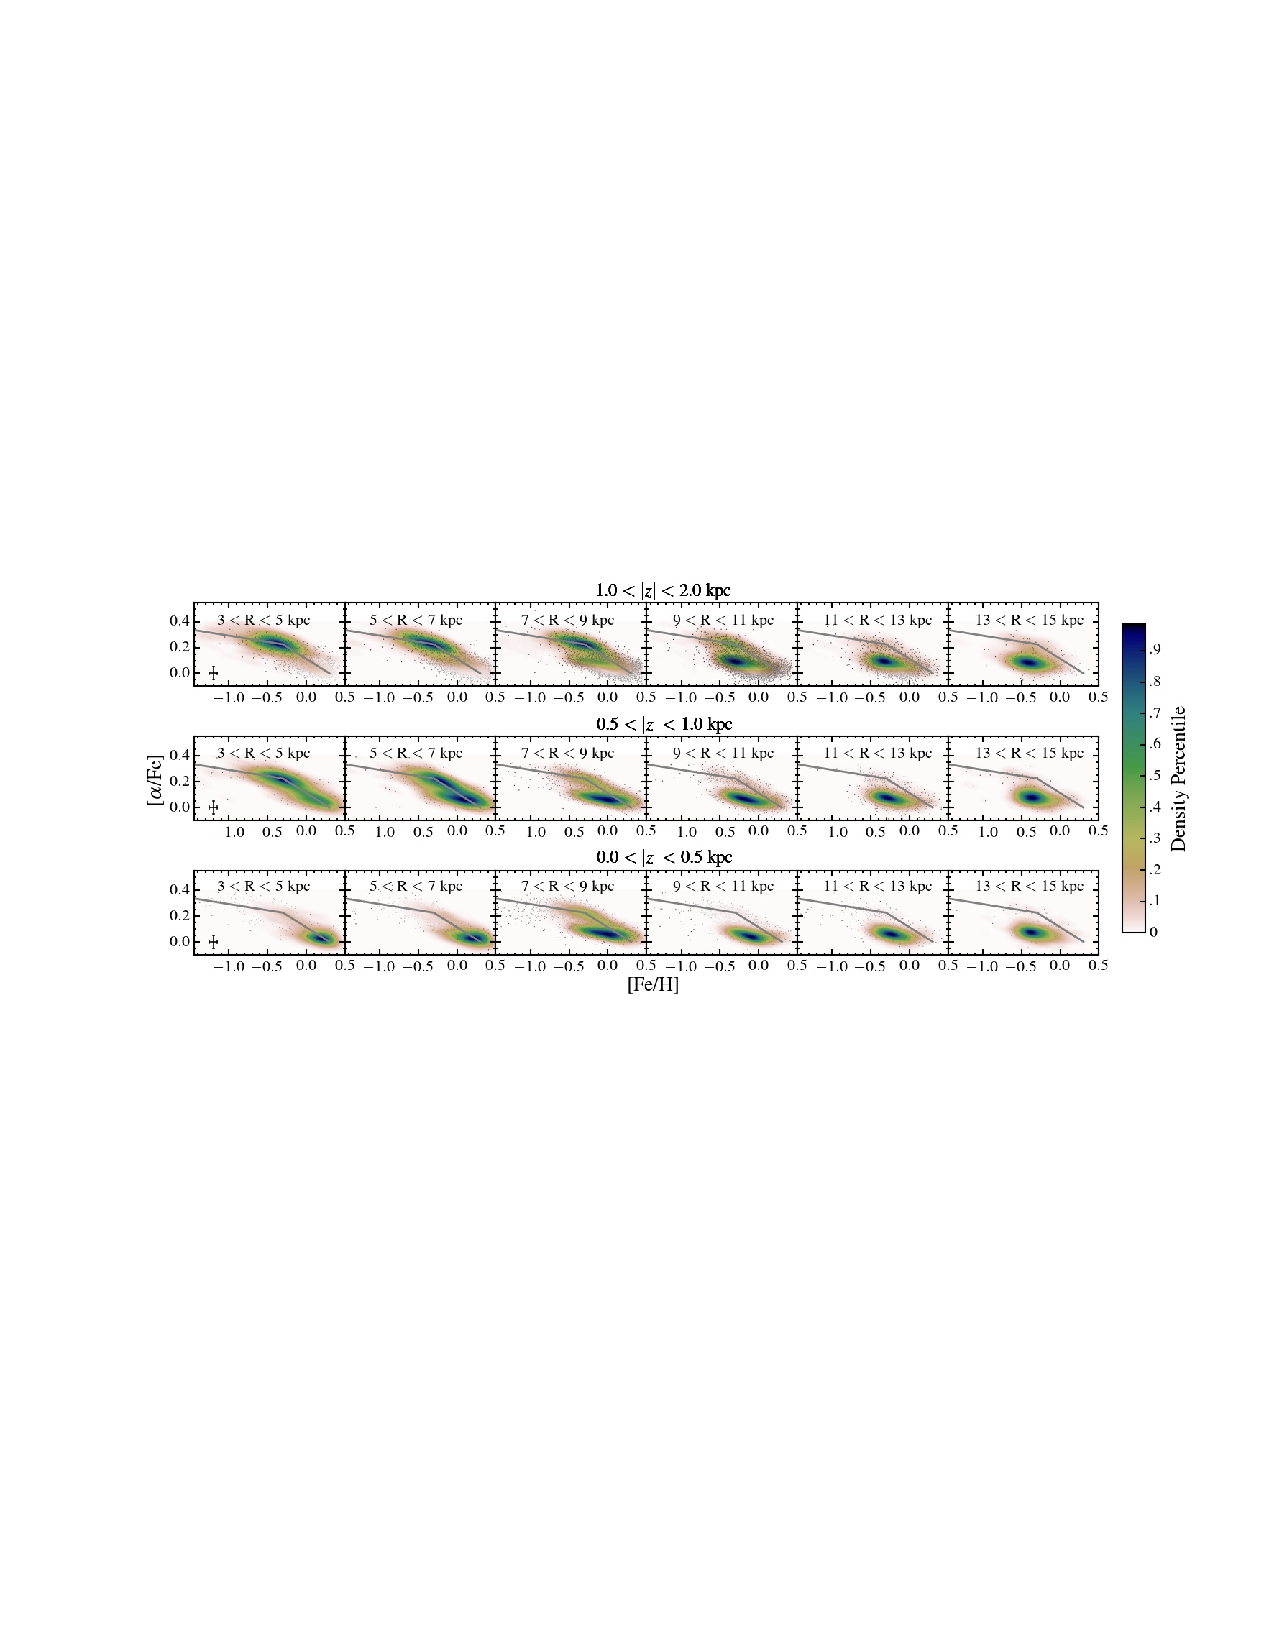
\includegraphics[width=\textwidth]{Introduction/figs/hayden_15.pdf}
  \caption[Metallicity and abundance of solar cylinder stars as a
  function of radius and
  height]{\fixspacing\label{intro:fig:hayden}The distribution of stars
    near the Sun in the [$\alpha$/Fe] vs. [Fe/H] plane, presented in a
    grid of radius and height. From \citet{Hayden15}.}
\end{figure}

By the middle of the last century it was well established that the
scale-heights and velocity dispersions of stars in the solar
neighborhood increase with age \citep[see][for a summary of this early
work, particularly the chapters contributed by Elvius and
Delhaye]{Blaauw65}. The seminal work by \citet{Roman50} demonstrated
that the disk kinematics also depended on metallicity.  Today these
patterns are known in the literature on Galactic archaeology as
age-velocity-metallicity (abundance) relations \citep[AVM$\alpha$-R;
e.g.,][]{Aumer09,Minchev14}. Observational advances continued for the
solar neighborhood \citep[e.g.,][]{Edvardsson93, Dehnen98,
  Nordstrom04}, and by the beginning of this century the complexity of
these relations had been mapped throughout much of Milky Way (MW) by
wide-field spectroscopic surveys (e.g., RAVE, \citealt{steinmetz06a};
BRAVA, \citealt{howard08a}, SEGUE, \citealt{yanny09a}, LAMOST,
\citealt{zhao12a} GALAH, \citealt{desilva15a},
Gaia-ESO,\citealt{gilmore12a}; and APOGEE-1 and -2,
\citealt{Majewski15}). The radial gradients in these relations are
beautifully shown in Figure \ref{intro:fig:hayden} (from
\citet{Hayden15}), illustrating the usefulness of both metallicity and
abundance as well-known, complementary chemical-evolutionary
tracers. Despite a century of remarkable progress, two broad but
intertwined questions remain: (i) What are the astrophysical processes
(i.e., the chemo-dynamical explanation) leading to the observed
relations?; and (ii) are these patterns generic for spiral disks or
specific to the Milky Way?

\begin{figure}
  \centering
  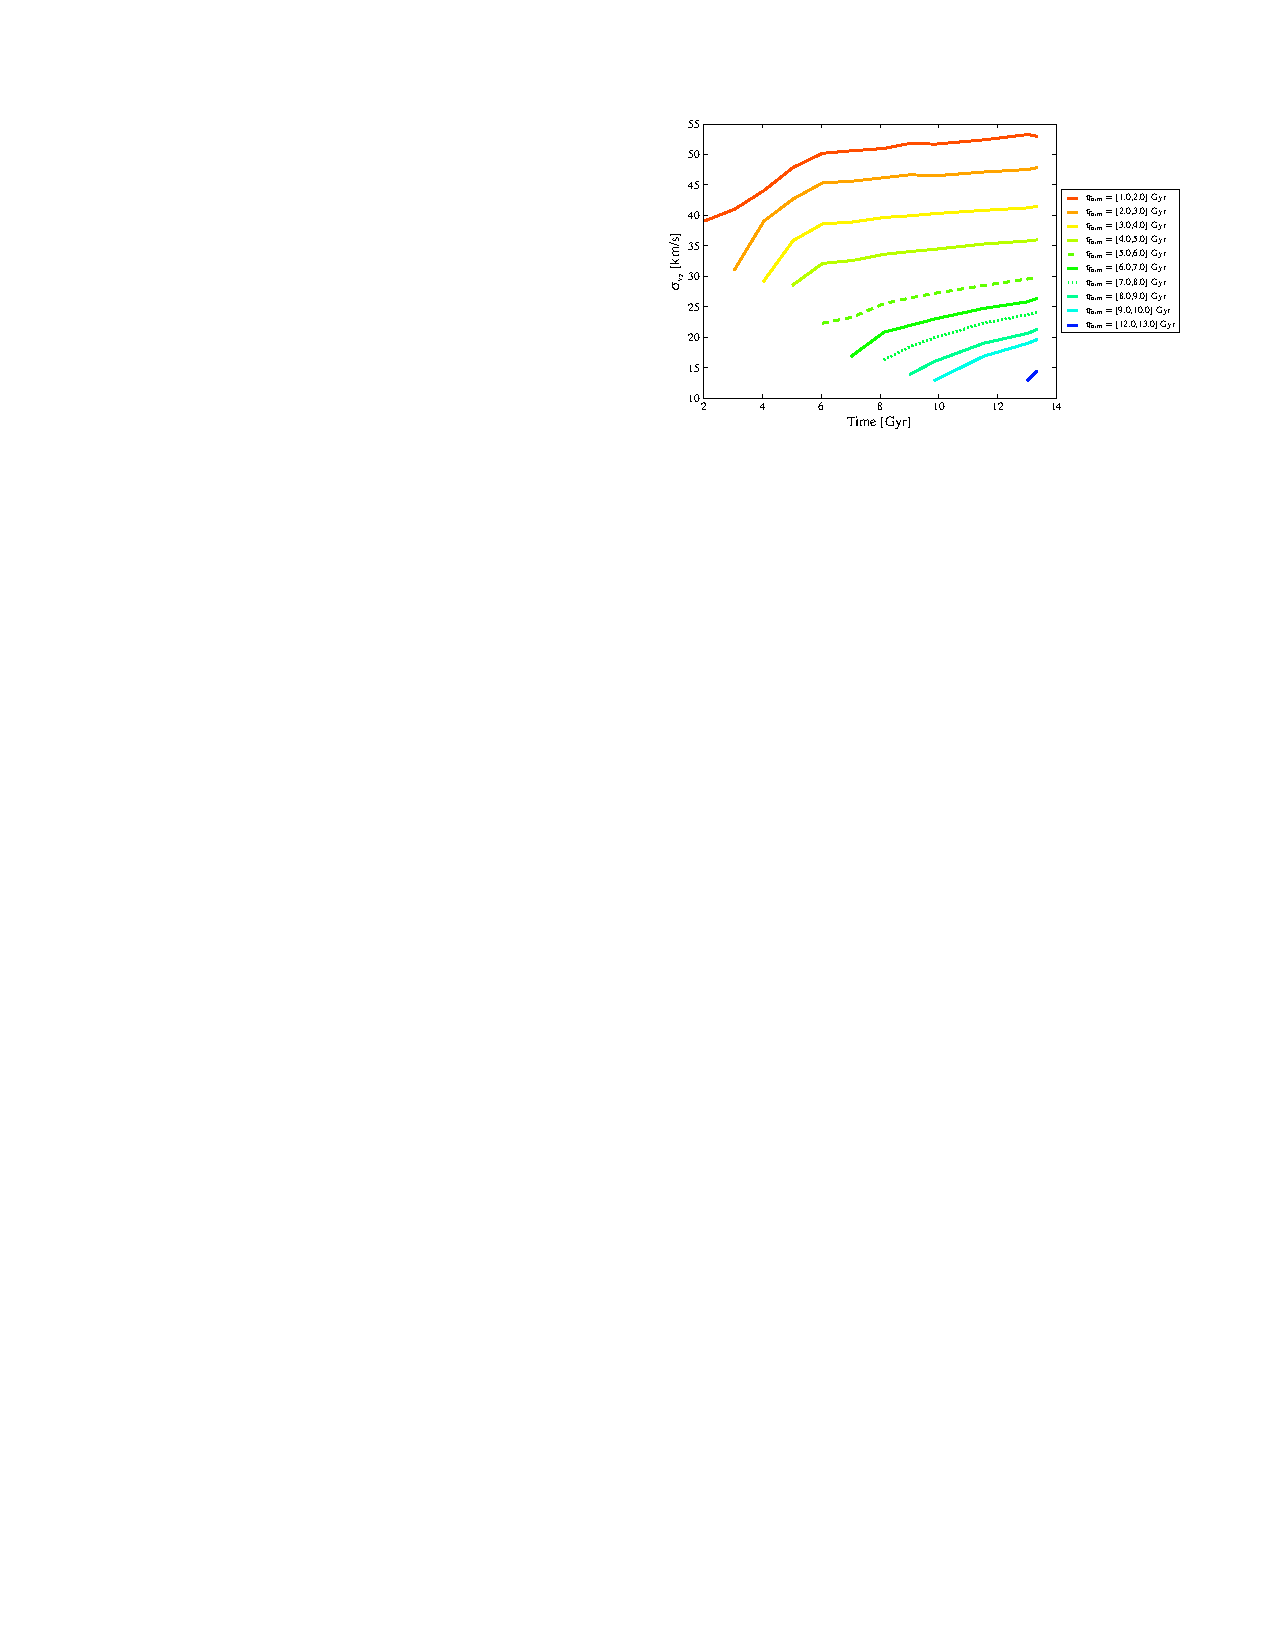
\includegraphics[width=0.8\textwidth]{Introduction/figs/bird_13.pdf}
  \caption[Dynamical settling in a Milky-Way-like galaxy
  model]{\fixspacing\label{intro:fig:bird}Vertical velocity dispersion
    of stellar populations with different formation ages as a function
    of time. These models are based on hydrodynamical simulations of a
    Milky-Way-like disk galaxy. From \citet{Bird13}}
\end{figure}

Setting aside chemical evolution for simplicity, there has been a
long-standing debate about the origin of the vertical stratification
of disk stars in phase-space as a function of age. This stratification
is known as the the age-velocity relation, or AV-R. Historically the
argument has been in the context of dynamical heating from two-body
scattering \citep{Spitzer51}, but the source of this scattering has
been debated \citep[e.g., giant molecular clouds, transient spiral
structure, or dwarf satellite
galaxies][]{Spitzer51,Spitzer53,Wielen77,Quinn93,Binney00}, and none
have proven satisfactory to explain the MW's thick disk.  This
framework has been salvaged but also up-ended by relatively recent
evidence for the increasing turbulence (and presumably thickness) of
ionized gas in disks at higher redshifts
\citep{Weiner06,Forster-Schreiber09,Wisnioski15}. It seems plausible
that early phases of disk formation involved gas cooling, leaving
behind an old, thick-disk stellar component
\citep{Brook04,Bournaud09}. However, thinner relic layers would also
emerge as time progressed \citep{Bird13}, depending critically on the
cooling time-scale for the gas in the presence of star-formation, AGN
feedback, and accretion. Figure \ref{intro:fig:bird} shows an example
of this theory; vertical velocity dispersion does slightly increase as
stars age (i.e. ``heating''), but the dominant trend is that more
recently formed populations are dynamically cooler. Ironically, this
``settling'' of the stellar disk is not unlike the predictions of
monolithic collapse from \citet{ELS}, albeit now consistent in the
context of bottom-up, or hierarchical structure formation as seen in
recent simulations \citep[e.g.,][]{Bird13,Martig14a}.  It is no longer
clear if, loosely speaking, disks ``heat'' or ``cool'' to form the the
vertical stratification of disk stars in phase-space, and likely both
modes play a role at late and early times, respectively. For this
reason we refer instead to ``dynamical stratification'' as a
phenomenon that captures both general physical processes.

The recent simulations noted above show there is a rich history of
radial and vertical build up of stellar populations that involves an
interplay between the cooling of the gas, the impact of mergers and
accretion, and, at late times, the classical heating processes noted
above.  This richness suggests the possibility for a diversity of
astrophysical paths in disk formation that could lead to significantly
different structure in galaxies, exhibited in their
AVM$\alpha$-Rs. Hence, the broader question of whether the MW is
representative of the external disk galaxy population becomes salient.

%% Maybe move to previous section
Little is known about the dynamical stratification rates for stars in
spiral galaxies outside the Milky Way, but recent studies of stellar
populations and dynamical stratification in low-mass spiral galaxies
\citep{Seth05a,Bernard15} have shown dramatic differences in the
age-metallicty and age-velocity dispersion relations when compared to
the Milky Way. Recent measurements of the stellar velocity dispersions
in M31 \citep{Dorman15} show that there are gradients in dispersion
with age and metallicity, but with amplitudes and time-scales that are
larger than in the MW. Differences in velocity dispersion amplitudes
may reflect a more massive or thinner M31 disk, but possibly also a
different dynamical history -- for gas settling or stellar dynamical
heating. Clearly more data on the stellar properties of external
galaxies is needed. The above studies serve as a gold standard since
they are based on studies of resolved stellar populations. Because
there are no massive spiral galaxies outside of the Local Group for
which we can resolve stellar populations at surface-densities high
enough to probe most of the disk, it is imperative to undertake
studies based on integrated starlight.

\section{Deriving Population Properties with Full Spectrum Fitting}
\label{intro:sec:SSP}
\begin{figure}
  \centering
  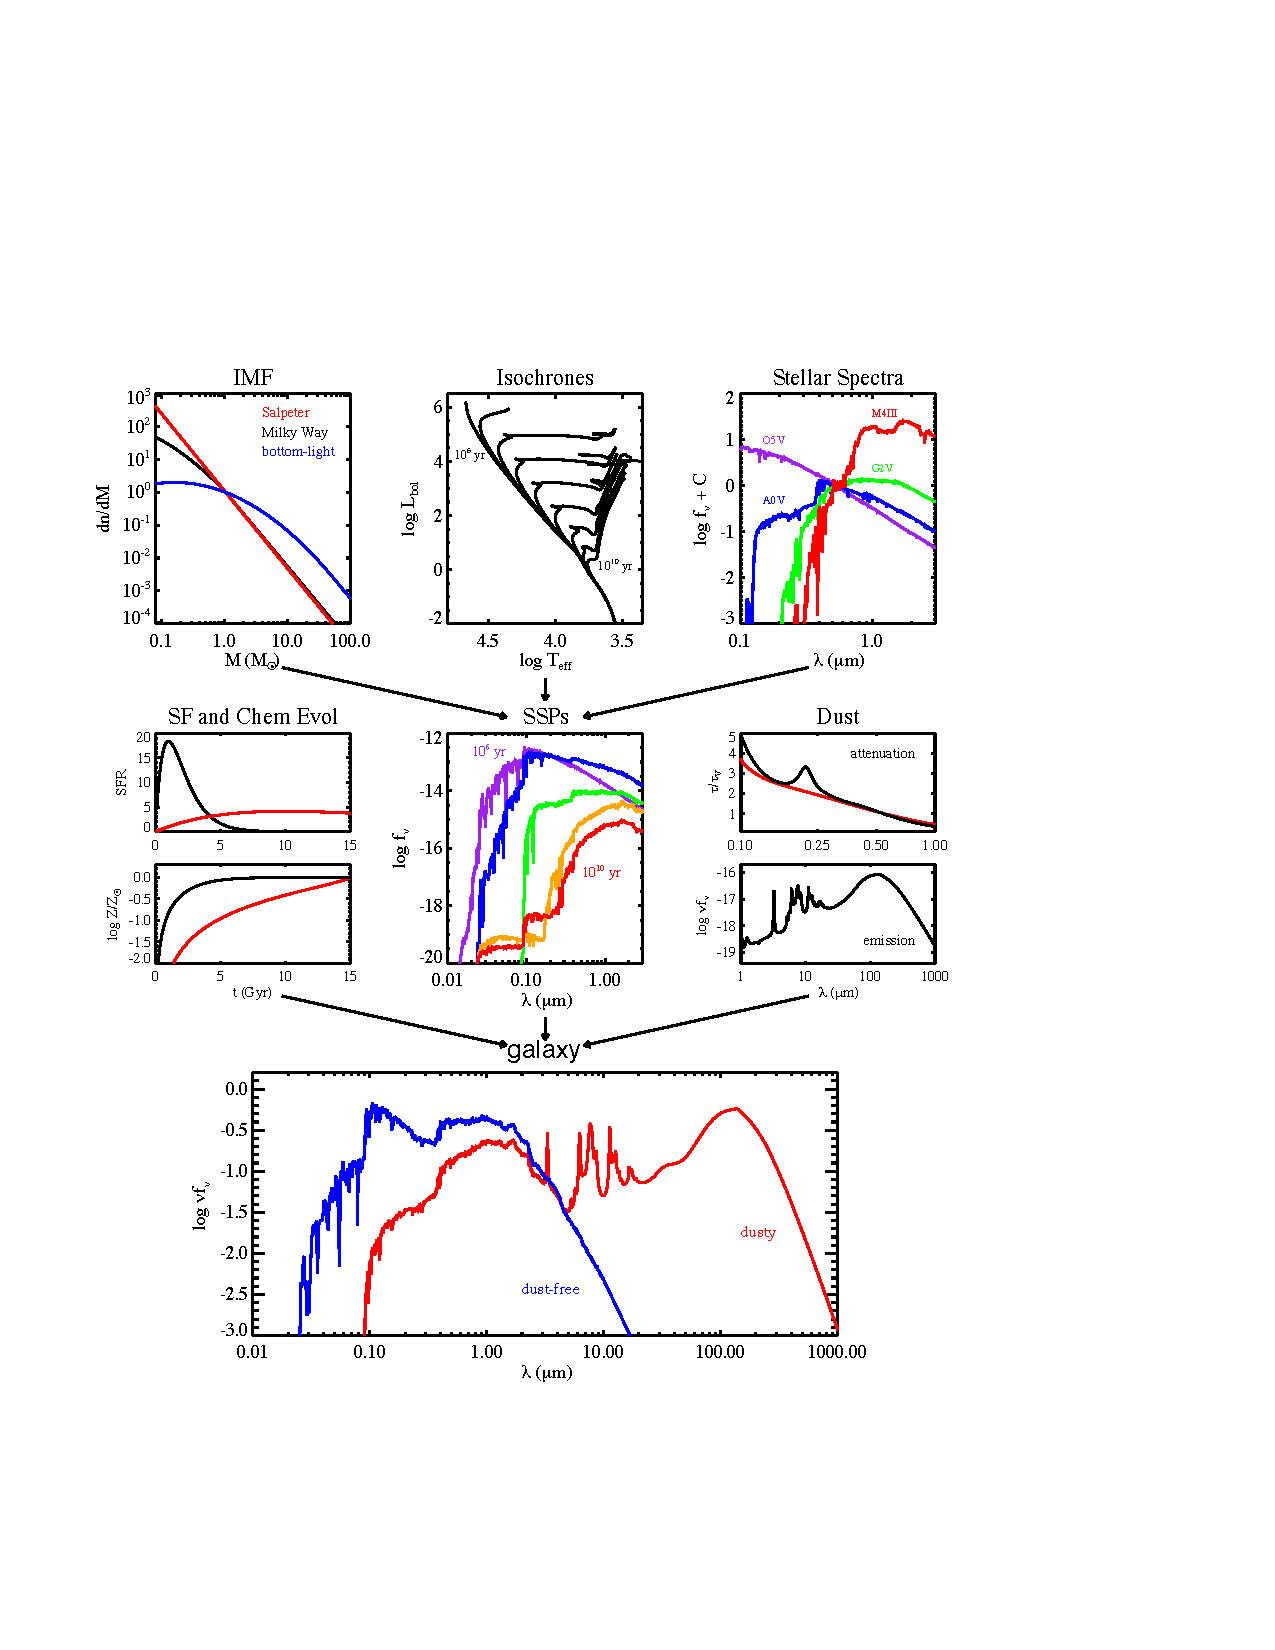
\includegraphics[width=0.8\textwidth]{Introduction/figs/conroy_13.pdf}
  \caption[Schematic of full spectrum
  fitting]{\fixspacing\label{intro:fig:conroy}The important components
    of full spectrum fitting. An initial mass function (IMF),
    isochrones, and spectra are combined to construct individual
    SSPs. Multiple SSPs are then combined, with and assumed star
    formation history and dust properties, to form a model
    galaxy. From \citet{Conroy13}.}
\end{figure}

In this work we employ full-spectral fitting to measure age,
metallicity, and extinction as a function of radius and height in NGC
891. The idea of modeling integrated starlight (i.e., a spectrum) to
measure galaxies properties has a long history since \citet{Spinrad71}
first manually mixed stars together, and modern techniques employ a
variety of sophisticated methods to extract the maximum about of data
from each wavelength. Regardless of the specific method, all attempts
at full-spectrum fitting require the same basic ingredients: (i) a
library of stellar spectra, whether empirical or synthetic, (ii) a set
of isochrones that encapsulate how stars evolve with time, and (iii)
an initial mass function (IMF). With these three components
Astronomers can construct simple stellar populations (SSPs); a set of
stars of the same age and same metallicity/abundance with a mass
distribution determined by the IMF. To simulate an entire galaxy
multiple SSPs of different ages and metallicities are combine together
to produce a complex stellar population (CSP), which requires assuming
both a star formation history (SFH) and the distribution/properties of
dust in the galaxy. An excellent discussion of this process can be
found in \citet[and his diagram shown in Figure
  \ref{intro:fig:conroy}]{Conroy13}.

Within the general picture painted above there exists a wide range of
options and data. It is common for SSP libraries to be constructed
with the Padova isochrones \citep{Bertelli94, Girardi00, Marigo08}
because these models cover the widest range of stellar age and
chemical compositions, but other models are often used for their focus
on specific epochs of stellar evolution. For example high-mass stars
(Geneva \citep{Schaller92,Meynet00}), low-mass stars ($Y^2$
\citep{Yi01,Yi03}, or Dartmouth \citep{Dotter08}), and even very
low-mass stars (Lyon \citep{Chabrier97,Baraffe98}). In this work we
use exclusively the Padova isochrones because our observations, by
their very nature, are light-weighted and therefore the specific
details of low mass stars are relatively unimportant.

The choice of IMF can also affect the final modeled galaxy
spectrum. The canonical IMF of \citet{Salpeter55} was based on
observations of the Solar Cylinder in the Milky Way, and there is so
far little evidence that the IMF is appreciably different elsewhere in
the Universe \citep{Bastian10}. More recent observations have refined
the specific form of the IMF \citep{Kroupa01, Chabrier03}, but the
general picture remains the same. We use the IMF of \citet{Chabrier03}
because it is physically motivated and provides a good fit to low-mass
and brown dwarf star counts in the Milky Way
\citep{Bruzual03,Chabrier01,Chabrier03}.

Finally, the construction of SSPs depends on the stellar library
used. In this work we consider only empirical stellar libraries, and
more specifically the STELIB \citep{LeBorgne03} and MILES
\citep{Sanchez-Blazquez06} libraries. The main strength of empirical
libraries is that they get the chemistry right by default, as indeed
they must. The cost of this accuracy, however, is a very limit
sampling of the entire parameter space of stellar evolution. For
example, as is discussed in \S\ref{891_2:sec:ma11}, the MILES library
very coarsely samples the metallicty/age plane and doesn't have any
spectra for ages below \val{6.5}{Myr}. 
% Ultimately, we use the STELIB
% library because it more finely samples stars of different ages, but
% warn that it still lacks a detailed view of how spectra change with
% metallicity.
As discussed in \S\ref{891_2:sec:SSP_sets} we ultimately use the SSPs
of \citet{Bruzual03}, which are constructed with the Padova
isochrones, Chabrier IMF, and STELIB library. We note, however, that
over the wavelength range we consider ($\val{3800}{\AA}
\leq\lambda\leq \val{6800}{\AA}$) the differences in spectral shape
caused by different assumptions/models are minimal.

More directly relevant to our work is the assumption about the SFH
that is used to construct galaxies (CSPs) from SSPs. A common choice
for SFH is the so called $\tau$-model where the star formation rate
(SFR) follows an exponential function with a single scale parameter,
$\tau_\mathrm{SF}$. This analytic form is based on closed-box models
where the SFR depends linearly on gas density \citep{Schmidt59} and
offers an attractive, one parameter, parameterization of the SFH. In
this work we chose to use a non-parametric SFH (as discussed in
\S\ref{891_2:sec:SSP_method}) which allows us to reduce the
systematics in our results that arise from forcing an analytic form of
the SFR (systematics are not completely eliminated, however, as
discussed in \S\ref{891_2:sec:sys_err}). Using this method results in
a much larger set of free parameters and puts more strain on the
fitting code, but our data have high enough signal to noise
(\val{\asim 30}{px^{-1}}) to make it a viable option.

Once model galaxies are constructed there are a multitude of methods
available to fit them to our data, for example those of
\citep{Cappellari04, Tojeiro07,Chen12, CidFernandes05, Ocvirk06,
  Wilkinson15, Sanchez16}. Regardless of the method used these fits
face the same common issues; namely how to deal with known
degeneracies between age, metallicity, and extinction
\citep{Oconnel76,Aaronson78,Worthey94,dePaz02}. In some methods the
extinction degeneracy can be mitigated by removing the overall
continuum from both the data and models before fitting
\citep[e.g.,][]{Ocvirk06,Wilkinson15} and then recovering an
extinction estimate either by measurements of gas emission (i.e., the
Balmer decrement) or separate analysis of the ``best fit'' galaxy
spectrum. Metallicity and age are more closely entwined and the
degeneracy between them more difficult to break. In this work we
attempt to quantify the uncertainties that arise from similarities
between SSPs that are degenerate with age and metallicity (see
\S\ref{sec:fit_err}), but note that we have not addressed systematic
uncertainties that may arise from our choice of model SSPs.

\section{A Fiber Optic Primer}
\label{intro:sec:fiber}
The use of fused silica optical fibers for astronomical observations
was first suggest by \citet{Angel77}, and in the intervening decades
their importance and usefulness to Astronomy has only increased. The
astronomical benefits of fiber optics are essentially two fold:
Firstly, they allow instruments to be decoupled from the telescope
focal plane, which enables the construction of very large and
sensitive spectrographs that are free from the unstable environmental
conditions often found on the observing floor. Secondly, they can be
easily placed at an arbitrary position on the sky while maintaining a
consistent spectrograph input.

A class of fiber optic instruments called integral field units (IFUs)
make great use of this second point. IFUs are a collection of fibers
that are placed in some two-dimensional configuration on the sky and
therefore produce data that exist in three dimensions (two spatial and
one spectral). Some IFUs are designed to efficiently measure the
spectra of a large field of stars, for example HYDRA {\bf REF? Can't
  find it!}, and can have the location of their fibers changed from
program to program. Others have a fiber layout that is fixed and
usually intended for observations of extended objects. SparsePak
\citep{Bershady04,Bershady05} is an excellent example of and IFU of
this type. The trade off for the lack of reconfigurability in fixed
IFUs is a generally tighter fiber packing and therefore improved
spatial coverage.

In the past, difficulties in construction resulted in a cottage
industry of IFU builders, but more recently there has been an
explosion of mass-produced IFUs that have allowed large, resolved
spectrographic surveys like MaNGA \citep{Bundy15}, SAMI
\citep{Croom12}, and CALIFA \citep{Sanchez12} to rapidly expand our
view of the Universe. In this thesis I present \GP and HexPak, a set
of IFUs that are the first in the world to contain fibers of different
sizes, each configured to serve a specific scientific purpose.

\begin{figure}
  \centering
  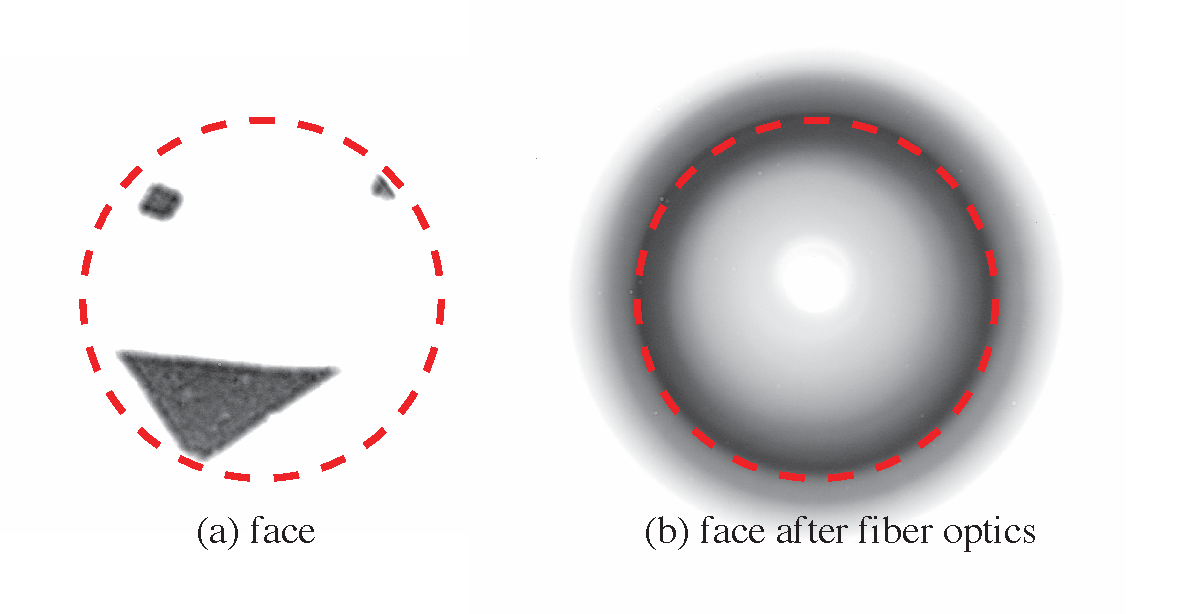
\includegraphics[width=\textwidth]{Introduction/figs/FRDude.pdf}
  \caption[Face on FRD]{\fixspacing\label{intro:fig:FRDude}The effects
    of fiber optics on an input signal. The face in (a) is smeared
    azimuthally and radially during its journey through an optical
    fiber. The red circle corresponds to the same angle at the
    input/output of the fiber.}
\end{figure}

With great power comes great responsibility, however, and fiber optics
affect the light passing through them in ways that have profound
implications for data quality and instrument design. In particular,
fiber optics not only attenuate precious astronomical light, but also
increase the entropy in the beam. The latter effect is referred to as
focal ratio degradation (FRD), whereby light injected into a fiber at
a particular angle emerges from the fiber at a larger angle. An
example of this is seen in Figure \ref{intro:fig:FRDude}; the light
coming out of the fiber (b) has been smeared to angles outside of the
maximum input angle (red circle). This increase in entropy creates a
need for larger (and more expensive) spectrograph optics and can
decrease the total system throughput if not properly accounted for. An
understanding of the causes of FRD can help mitigate its effects and
the first theories placed the blame on microbends along the length of
the fiber \citep{Gloge72,Carrasco94}. Recent studies have suggested
however, that most FRD is caused by scattering at the surface of the
fiber \citep{Avila98,Haynes11,Eigenbrot12}. In the latter scenario it
is likely that surface treatments (i.e., anti-reflective coatings) can
mitigate the effects of FRD.

\clearpage
\phantomsection % Fixes references link in hyperref/PDF index

% Requires thesis.bst to be present (or linked) in chapter subdirectory.
\bibliographystyle{thesis}
\bibliography{Introduction}

\chapter[Fiber Focal Ration Degradation]{The Angular and Wavelength Dependence of Fiber Focal Ratio Degradation}
\label{chap:FRD}
\epigraph{\fixspacing\emph{Every hidden cell is throbbing with music
    and life, every fiber thrilling like harp strings.}}{John Muir}
% Leave space between title and quote or publication note.  This has often been
% 10cm for a quote and 8 cm for a reference, but this is really up to you.
%\vspace{8cm}
\vfill

\begin{flushright}
  \fixspacing
  \textit{A version of this chapter has previously appeared in\\
    \emph{Ground-based and Airborne Instrumentation for Astronomy IV. Proceedings of the SPIE}}\\
    \vspace{1ex}
    Eigenbrot, Bershady, and Wood 2012. Volume 8446 article 84465W
\end{flushright}

\vspace{1in}

\cleardoublepage

%%%%%%%%%%%%%%%%%%%%%%%%%%%%%%%%%%%%%%%%%%%%%%%%%%%%%%%%%%%%% 
\begin{chabstract}
  We present measurements of how multimode fiber focal-ratio degradation
  (FRD) and throughput vary with levels of fiber surface polish from 60
  to 0.5 micron grit. Measurements used full-beam and laser injection
  methods at wavelengths between 0.4 and 0.8 microns on 17 meter lengths
  of Polymicro FBP 300 and 400\mum\ core fiber. Full-beam injection
  probed input focal-ratios between \f3 and \f13.5, while laser
  injection allowed us to isolate FRD at discrete injection angles up to
  17 degrees (\f1.6 marginal ray). We find (1) FRD effects decrease as
  grit size decreases, with the largest gains in beam quality occurring
  at grit sizes above 5\mum; (2) total throughput increases as grit
  size decreases, reaching 90\% at \filtI with the finest polishing
  levels; (3) total throughput is higher at redder wavelengths for
  coarser polishing grit, indicating surface-scattering as the primary
  source of loss. We also quantify the angular dependence of FRD as a
  function of polishing level. Our results indicate that a commonly
  adopted micro-bending model for FRD is a poor descriptor of the
  observed phenomenon.
\end{chabstract}
\cleardoublepage

\section{Introduction}

Multimode optical fibers provide the most cost-effective coupling
between telescopes and spectrographs that allow spectrographs to be
placed in stable environments. However, these fiber optics contribute
to light loss from attenuation within the fiber material and
surface-scattering of their ends, and increase entropy in the optical
beam. The latter effect is referred to as focal ratio degradation
(FRD), whereby light injected into a fiber at a particular \fratio
emerges at a faster (smaller) \fratio. Ever since the first efforts to
characterize FRD in astronomical applications \citep{Angel77}
astronomers have attempted to understand its cause(s) in the hope to
lessen its effects \citep{Carrasco,Oliveira}. Microbends have
historically been a favored culprit \citep{Carrasco,Gloge72}, but
recently it has been suggested \citep{Haynes11, Avila98} that scattering
caused by surface-roughness on the fiber face contributes
significantly to FRD.

We discuss the results of two experiments designed to measure how the
amount of FRD depends on surface roughness, wavelength, and input
angle. The experiments described here use both full-beam and laser
injection methods \citep{Carrasco} standard for FRD tests in
astronomical applications. The full-beam method is useful for
characterizing how a fiber would perform when fed by a telescope,
and provides a straightforward way to compute practical metrics useful
for designing spectroscopic instruments. The laser injection method
allows light to be injected into the fiber at discrete input angles
(compared to a filled ray-bundle cone). This angular dependence of
scattering is a particularly sensitive diagnostic of the physical
mechanisms responsible for FRD.

The method and results of our experiment of FRD dependence on surface
roughness are presented in \S \ref{FRD:sec:polish}. Results for the
wavelength dependence of FRD are reported in \S
\ref{FRD:sec:wavelength}. The dependence of scattering on input angle is
reported in \S \ref{FRD:sec:angle}, and the implications of our work are
discussed in \S \ref{FRD:sec:summary}.

\section{Grit Size and Wavelength Dependence}
\label{FRD:sec:polish}
\subsection{Polishing Method}
\begin{figure}[ht]
    \includegraphics[width=1.0\textwidth]{FRD/figs/mosaic.eps}
    \caption[Fiber face with varying degrees of polish]{\fixspacing Images of
      the ``test'' surface of the fiber cable showing the appearance of the
      fiber face at each of the six stages of polishing. The number in the
      bottom right corner of each panel denotes the size of grit used. The
      fiber core diameter is 300$\mu$m.\label{fig:mosaic}}
\end{figure}

Our tests used Polymicro Technologies stepped-index broadband optical
fibers, cut to $\sim$17 meters in length.  FBP300330370 has
core:clad:buffer diameters of 300:330:370\mum, respectively; a second
length of FBP400440480 has 400:440:480\mum\ diameters.  We mounted
each fiber end into 0.25 inch cylindrical brass ferrules using Norland
Optical Adhesive 61 ultraviolet-curing epoxy.

The experiment was designed to maintain one end of each fiber cable as
a ``control'' surface, well-polished (0.5\mum) at the beginning of
testing, and to use the other end of the fiber cable as the ``test''
surface, initially polished using a coarse grit and then re-polished
with successively finer grit sizes after each measurement.  For
creating the progression of decreasing surface roughness we performed
consecutive polishing steps on the test surface using silicon carbide
lapping disks of 60, 30, 15, 5, and 1\mum\ grit as well as 0.5
\mum\ grit aluminum oxide disks.

The fiber cable was polished using an Ultra Tec Manufacturing, Inc.,
ULTRAPOL 1200-series lapping machine.  We considered a fiber surface
to be adequately polished when, under visual inspection, surface
grooves appeared to be relatively even across the face with very few
surface features larger than the grit size used to polish the surface.
We imaged each end of the fiber using a Newport Corporation F-ML1
fiber inspection microscope for magnification and a Motic Corporation
Moticam 2300 CMOS detector.  We took images after each polishing step
in order to confirm that the test surface was adequately polished and
that the control surface remained undamaged.  We also captured images
after each FRD measurement step in order to determine if the fiber
faces had been damaged during handling, as any potential damage could
affect the test results.  A mosaic of images of the test surface, as
seen after the FRD measurement at each grit size, is seen in
Figure~\ref{fig:mosaic}.


\subsection{Data Collection}
\label{FRD:sec:direct}
The experimental apparatus is a modified version of the far-field
differential beam comparator using a double re-imaging system
described in \citet{Crause_08}, which is based of the FRD test
apparatus used to characterize the fibers of SPARSPAK
\citep{Mab_04}. The final collimating lens (L3 in \citet{Crause_08})
was replaced with a Canon \f1.2 camera lens to eliminate ghost images
caused by very fast output beams. Stray light was further reduced by
covering everything downstream of the focus plane with a black
photographer's cloth. The fiber input stage was replaced with a highly
stable, purpose-built three-axis translation stage that ensures the
fiber face is telecentric to within $0.01^{\circ}$. Finally, a filter
magazine was added to the pinhole assembly to facilitate the rapid
changing of filters.

Basic operation involves recording data from two imaging modes; the
far-field fiber output, and the far-field image of the direct
beam. The level of FRD is then computed by comparing the two modes.
Examples of these images are shown in Figure \ref{fig:dfim},
illustrating the increasing impact of FRD at slower beam-speeds. Data
were taken in three filters: Johnson I and B and Stromgren \emph{y},
with central wavelengths of \filtI, \filtB, \filty, and widths of
$\Delta\lambda/\lambda=$ 0.22, 0.19, 0.045, respectively; four
$f$-ratios (\f3, \f4.2, \f6.3, and \f13.5); and five polish
levels (60, 30, 15, 5, and 1\mum). The range in $f$-ratios was chosen
so that results are applicable to a wide range of telescope
designs. The Wisconsin Indiana Yale NOAO (WIYN) 3.5m telescope has a
\f6.3 Nasmyth port; the Sloan Digital Sky Survey Telescope fibers
are fed at \f5; and the South African Large Telescope (SALT) feeds its
prime focus instrument package at \f4.2 (similar to the Hobby Eberly
Telescope).

Throughput measurements require very precise knowledge of the
intrinsic lamp output (the light input to the system). Experiments in
lab showed that, while the stochastic variations of the lamp are
negligible, there is a secular drift towards lower lamp
output. Subsequent to the experiment reported here a photo-diode
monitoring system has been implemented to correct for this trend. The
data presented here accounted for this trend by: 1) taking a set of
images for one filter with the fiber in place, 2) taking a set of
direct beam images in the same filter, 3) repeating this alternating
scheme until three groups of fiber images, separated by two groups of
direct beam images were taken. This alternating fiber-direct-fiber
scheme is used to remove stochastic lamp variability.

Images were cleaned of detector artifacts and combined to produce five
images for each filter at each polish level: three fiber images and
two direct beam images. Lamp variations were removed by using the
three fiber images as data points to determine a lamp normalization
(relative to the first fiber image) as a function of time. This
function was then used to find normalizations for the direct beam
images. The lamp was found to have no significant variation (10\% of the shot noise)
 within the time required to take one set of data in a particular filter.

\begin{figure}[ht]
\centering
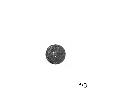
\includegraphics[width=0.25\textwidth]{FRD/figs/bdirect_3.eps}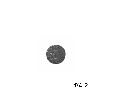
\includegraphics[width=0.25\textwidth]{FRD/figs/bdirect_42.eps}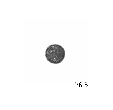
\includegraphics[width=0.25\textwidth]{FRD/figs/bdirect_63.eps}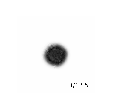
\includegraphics[width=0.25\textwidth]{FRD/figs/bdirect_135.eps}\\
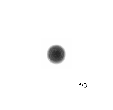
\includegraphics[width=0.25\textwidth]{FRD/figs/bfiber_3.eps}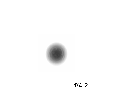
\includegraphics[width=0.25\textwidth]{FRD/figs/bfiber_42.eps}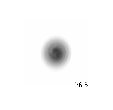
\includegraphics[width=0.25\textwidth]{FRD/figs/bfiber_63.eps}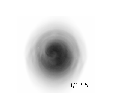
\includegraphics[width=0.25\textwidth]{FRD/figs/bfiber_135.eps}
\caption[Input and output far-field
  images]{\fixspacing\label{fig:dfim}Far-field images of the direct-beam (top)
  and fiber-beam (bottom) outputs for all $f$-ratios tested. Data shown is at
  \filty for the FBP300330370 fiber, 17m in length. Direct and fiber beam
  images for a given \fratio have identical spatial scales, and are adjusted
  such that the direct beam images are the same apparent size for all
  $f$-ratios.}
\end{figure}

\subsection{Analysis}
A custom data reduction pipeline was created to consistently and
efficiently analyze the large volume of data associated with the
multiple filters and polish levels. Analysis consisted of measuring
the total light contained within annuli of constant width and
increasing radius centered on the center of the beam. This information
was then used to construct a curve of growth that shows the fractional
encircled energy (EE) as a function of radius.

In addition to FRD, there are aberrations inherent in our test
apparatus that will affect both the direct beam and fiber beam in the
same way. To remove the effects of these aberrations the difference
between the direct beam and a theoretical ideal beam (no aberrations)
is computed and applied to both the fiber and direct beams;
\citet{Crause_08} provide a complete description of the method
used. Once the corrections have been applied the only differences
between the fiber and direct beams are caused by FRD.

\subsection{Results}
\label{FRD:sec:results}

\begin{figure}[ht]
\begin{center}
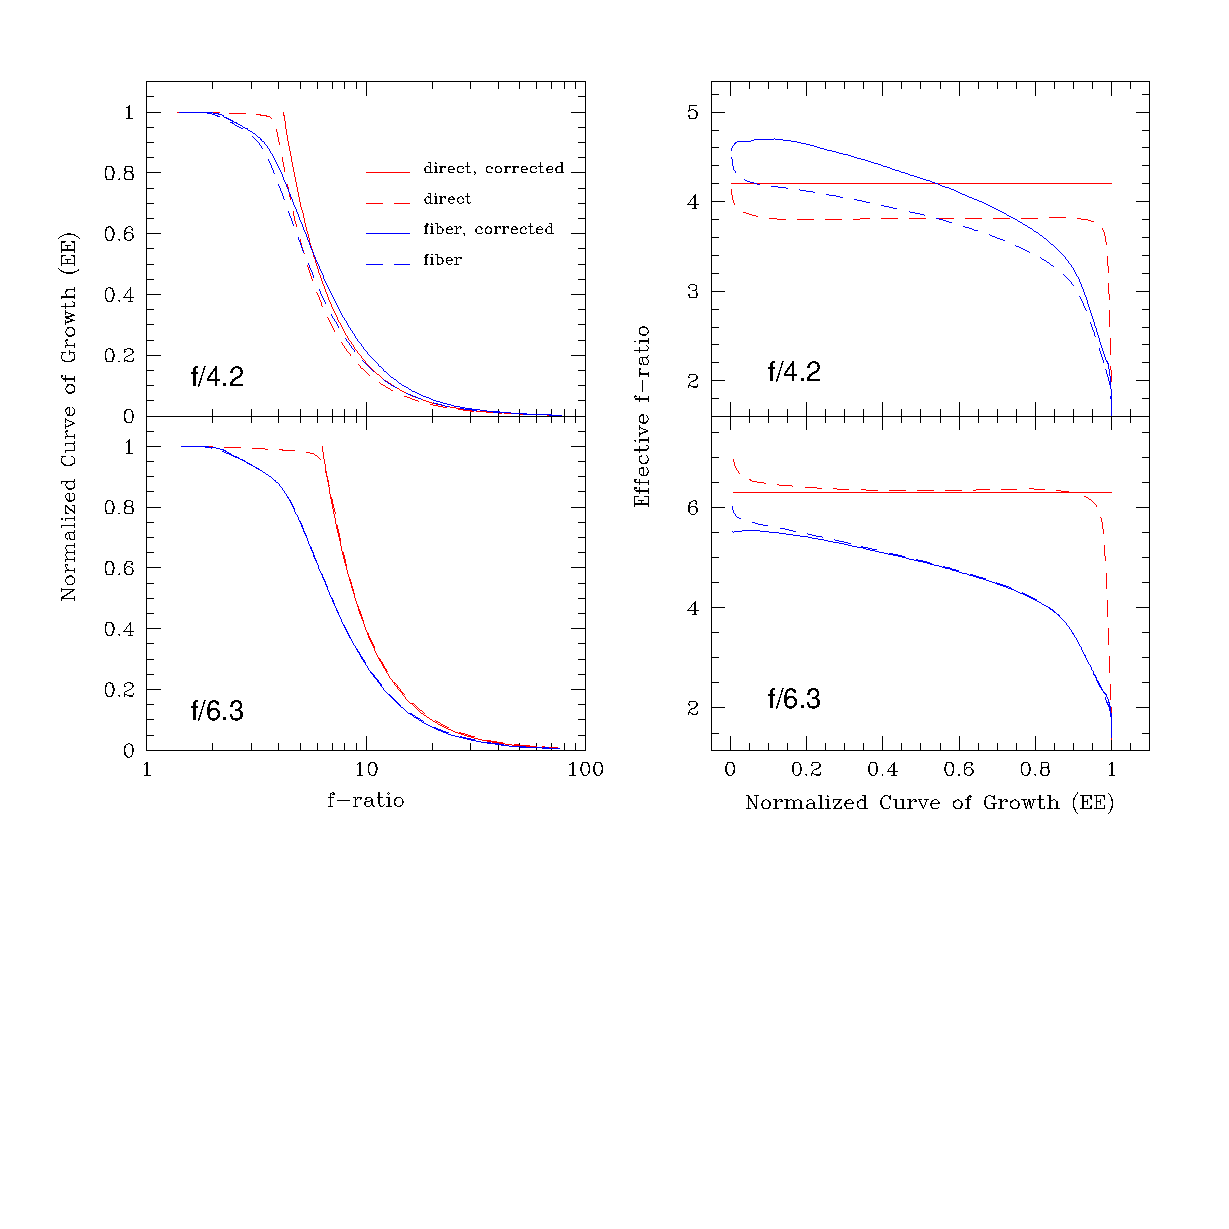
\includegraphics[width=\textwidth, trim=0 2.6in 0 0, clip=true]{FRD/figs/basic_FRD.eps}
\caption[Example FRD analysis plots]{\fixspacing\label{fig:basicFRD} FRD
  effects at \filty, \f4.2 and \f6.3, and with the output face polished to
  30\mum. The left panels show enclosed energy (EE) as a function of
  \fratio. The right panels show the effective \fratio of a beam that captures
  a certain percentage of the total light (EE). Data is for the FBP300330370
  fiber, 17m in length.}
\end{center}
\end{figure}

Figure \ref{fig:basicFRD} shows a characteristic set of FRD analysis
plots at a 30\mum\ end-polish at \f4.2 and \f6.3.  (See Figure
\ref{fig:grit} for more grit-sizes and \S\ref{FRD:sec:gritwave} for
discussion).  The left panels, which consist of normalized curves of
growth (COG) for both the direct and fiber beams, show how FRD
scatters light out to larger radii. The dashed and solid lines are the
data before and after the correction described above \citep{Crause_08}.

The right panels plot the effective \fratio as a function of
EE. These plots only show information about relative light
(re)distribution; they do not contain any information about total
throughput.  Where the fiber curve intersects the ideal beam tells us
what percentage of the original beam's information is being captured
by a spectrograph with an \fratio equal to that of the optics feeding
the fibers. This plot can also be used to estimate how much faster a
spectrograph would have to be to capture more of the input beam. For
example, from figure \ref{fig:basicFRD} and for fibers polished to 30\mum, an \f4.2
spectrograph only captures about 53\% of the light fed into the fibers 
at \f4.2. If we wanted to capture 90\% of the input light the
spectrograph optics would need to be \f3.2.

\subsubsection{Grit-size and \fratio Dependence}
\label{FRD:sec:gritwave}
\begin{figure}[htp]
  \centering
  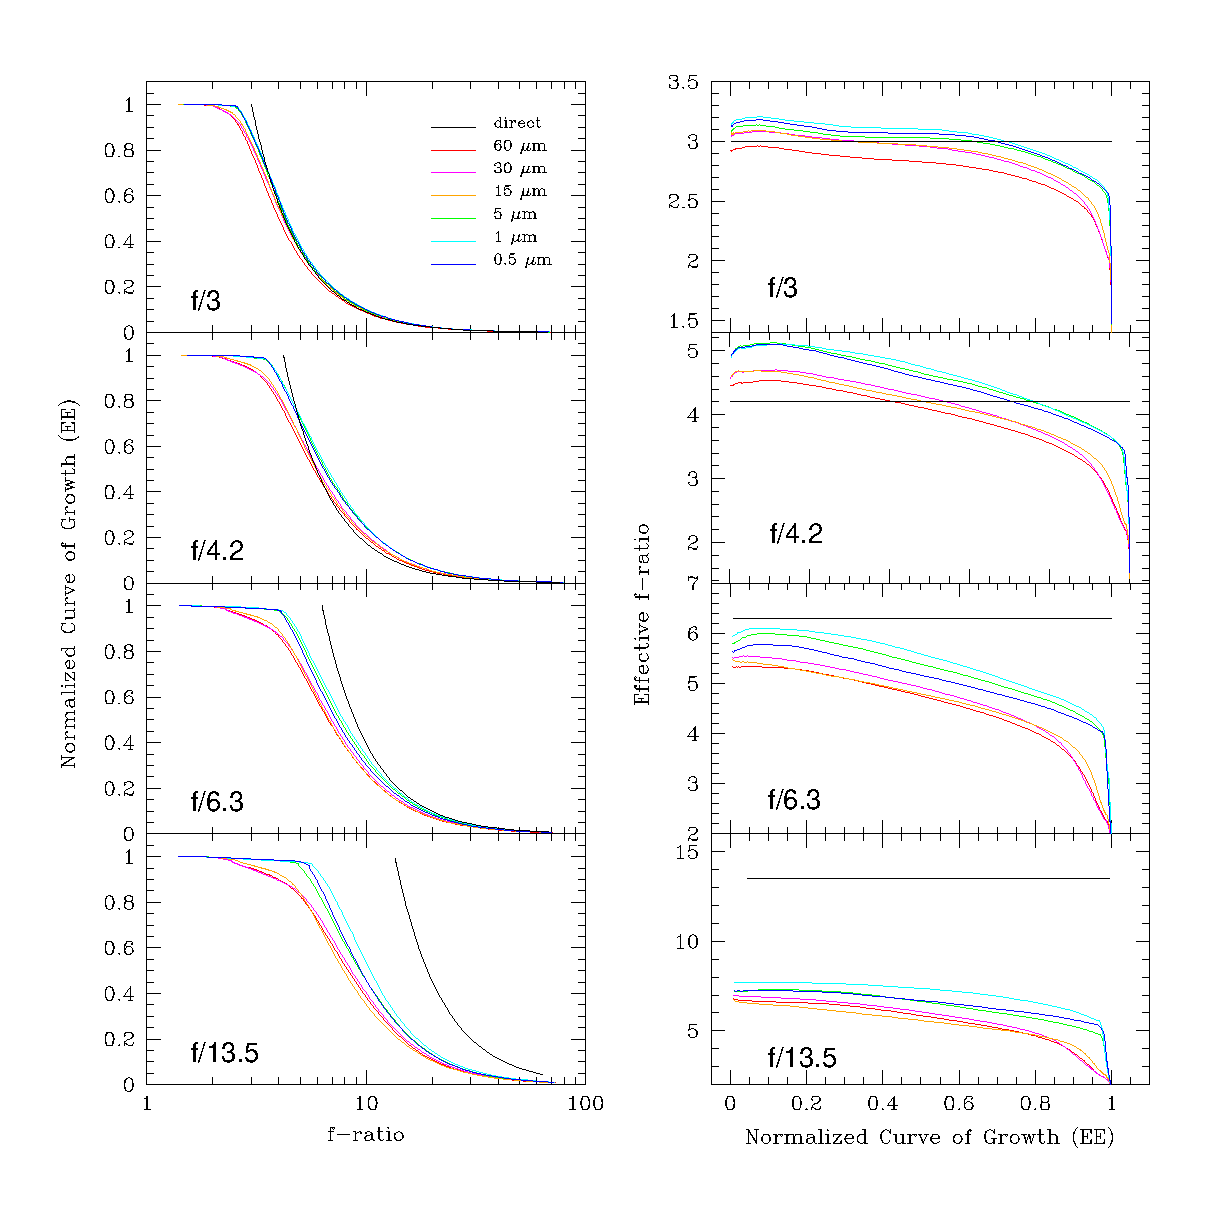
\includegraphics[width=\textwidth]{FRD/figs/gritplot.eps}
  \caption[Dependence of FRD on polish
    level]{\fixspacing\label{fig:grit}Dependence of FRD on polish grit size at
    \filty and all $f$-ratios measured for 17m of FBP300330370 fiber.}
\end{figure}

The primary result of the experiment can be seen in figure
\ref{fig:grit}, which shows FRD curves at one wavelength (\filty) and at
all of the different end-polish levels and $f$-ratios. As expected,
the effects of FRD improve as grit size decreases, but only to a
point. There is steady improvement in output beam quality between 60
\mum\ and 15\mum, a sharp improvement between 15\mum\ and 5\mum,
and almost no improvement between 5\mum\ and 0.5\mum.

It is also worth noting that for certain combinations of input \fratio
and polish level there is a radius (output \fratio) within which there
is relatively \emph{more} light in the fiber beam than in the direct
beam.  The explanation is straightforward: FRD scatters light from
each input angle into both larger and smaller output angles. If the
width of the scattering profile increases towards smaller angles (see
\S\ref{FRD:sec:angle}) then more light is scattered out of these angles
compared to larger angles. However, for a uniform input beam
larger input angles contain more luminosity (because they contain
larger annular areas) and so the amount of light scattered in from large
angles will exceed the amount of light scattered out from small angles
despite the wider scattering profile at small angles. In this case the
fiber beam will have relatively more light at smaller angles than the
direct beam, as seen in the plots for \f3 and \f4.2. Conversely,
there is some sufficiently large output angle that has
significant scattering contributions from angles where there is no
light in the input beam. At these output angles, the COG drops below
the ideal beam, as observed.

It is well known that FRD changes with changing input $f$-ratio,
increasing with slower beams \citet{Ramsey88}, as seen in Figure
\ref{fig:grit}.  For beams slower than \f6.3 the scattering becomes so
large that the output beam never contains more light than the input
beam for any angle.

\subsubsection{Wavelength Dependence and Total Throughput}
\label{FRD:sec:wavelength}
\begin{figure}[ht]
  \centering
  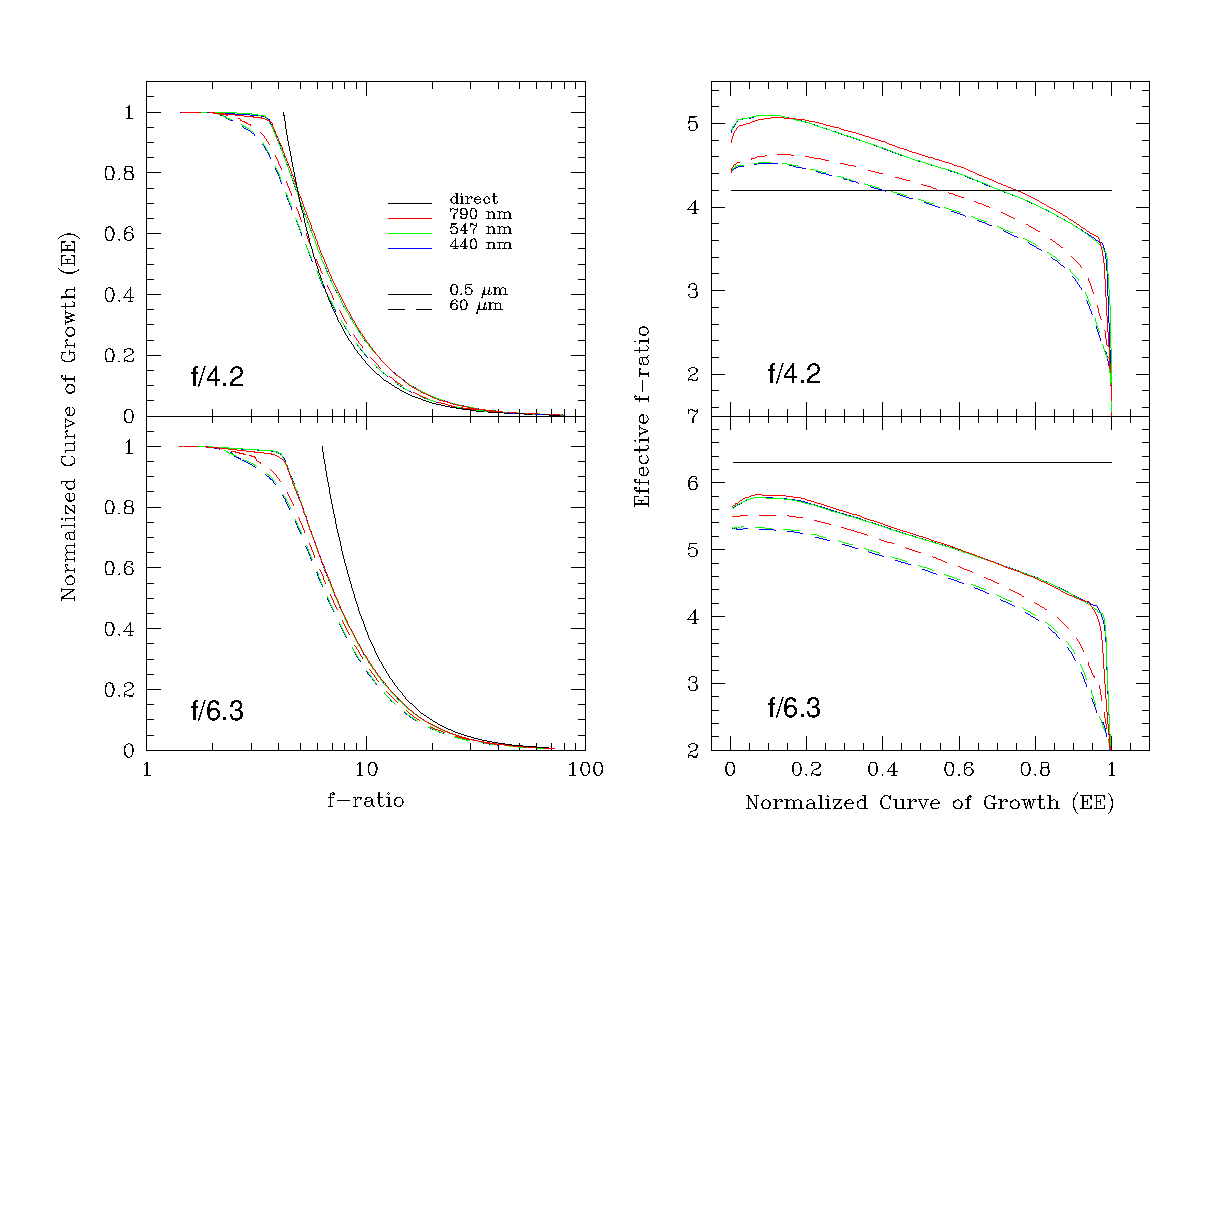
\includegraphics[width=\textwidth, trim=0 2.6in 0 0, clip=true]{FRD/figs/filters.eps}
  \caption[Dependence of FRD on wavelength]{\fixspacing\label{fig:wave}
    Wavelength dependence of FRD at 0.5 and 60 \mum\ polish grit at \f4.2
    and \f6.3 for 17m length FBP300330370 fiber.}
\end{figure}

Previous tests for a wavelength dependence on FRD have been split
between results that suggest there is such a
dependence \citep{Carrasco,Gloge72}, based on what would be predicted by
a micro-bend origin, and results that point to no wavelength
dependence \citep{Mab_04, Schmoll_03}. Figure \ref{fig:wave} shows FRD
curves for all filters at \f4.2 and \f6.3 and 0.5\mum\ and 60
\mum\ polish levels. The data suggest that at a fine polish level (0.5
\mum) the amount of scattering caused by FRD does {\it not} depend on
the wavelength of the input light. However, at 60\mum\ we do see some
wavelength dependence to the FRD curves, which  must therefore be
caused by surface scattering (see figure \ref{fig:tputwave}).

We also find that the total throughput of the fiber depends on
fiber polish. Figure \ref{fig:tputwave} shows the
total throughput as a function of grit size for all three wavelengths
and \f6.3. The total throughput is defined as the asymptotic (in output
 angle) fiber beam counts referenced to the same measurement of the direct
 beam. From the manufacturer's specifications
we expect the fiber attenuation to depend on wavelength. Polymicro
reports attenuations of 20 dB/km at \filtB, 10 dB/km at \filty, and 5
dB/km at \filtI, and we also expect a 3.43\% light loss from each
air-silica interface (input and output faces). Thus, in the case of an
ideal, \val{17}{m} long fiber we expect a throughput of 85.6\%,
89.3\%, and 91.2\% for \filtB, \filty, and \filtI, respectively. These
values are plotted as horizontal dashed lines in figure
\ref{fig:tputwave}. Any additional losses are likely due to surface
scattering.

We also find a polish dependence on the color of the transmission.  As
seen in the right panel of figure \ref{fig:tputwave}, the throughput
gains are greater at shorter wavelengths as the surface-polish
improves, as would be expected from a surface-scattering phenomenon.

\begin{figure}[ht]
  \centering
  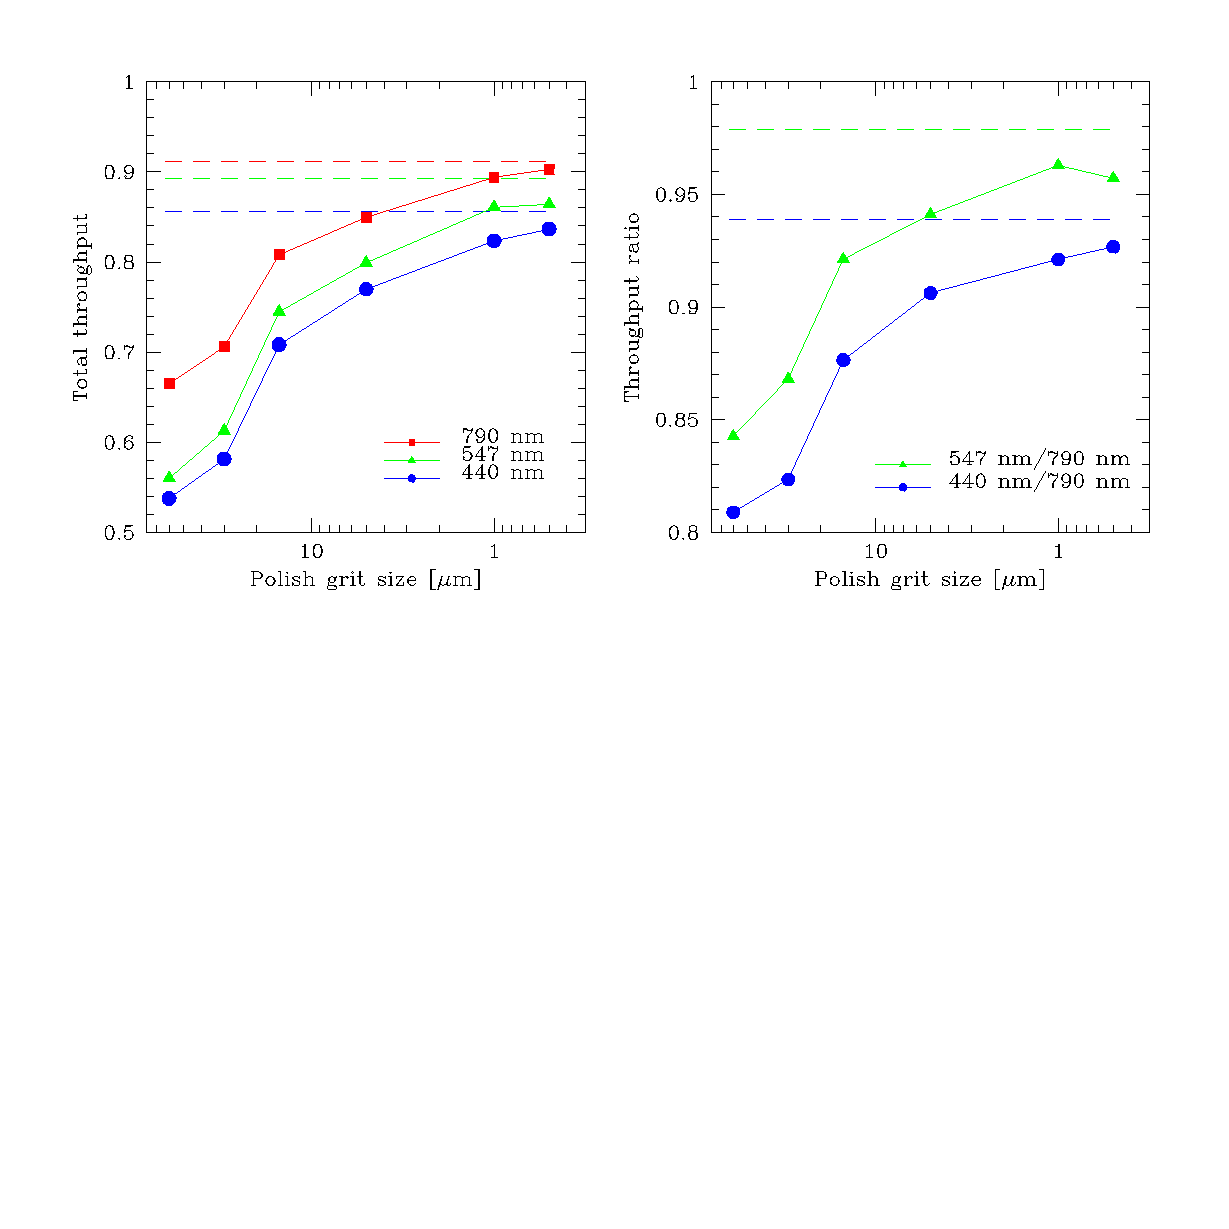
\includegraphics[width=\textwidth, trim=0 4in 0 0, clip=true]{FRD/figs/tput.eps}
  \caption[Total throughput as a function of wavelength and polish
    level]{\fixspacing\label{fig:tputwave} Total throughput as a function of
    polish grit for three different wavelengths (left), and the relative
    increase in \filtB and \filty referenced to \filtI (right). Dashed lines
    show the values expected from the product specifications. This is measured
    for a 17m length of FBP400440480 fiber.}
\end{figure}

\section{Angle Dependence}
\label{FRD:sec:angle}
\subsection{Experiment}
We are also interested in the dependence of FRD on the light input
angle. The direct beam injection method reported in
\S\ref{FRD:sec:direct} injects a full cone of light into a fiber,
i.e., the input beam contains rays incident on the fiber face from
normal up to half of the vertex angle of the cone.  To probe FRD
effects at single, discrete input angles (essentially an annular cone)
we use an experiment similar to the laser injection method of
\citet{Carrasco} and \citet{Haynes11}, but modified so that the far field fiber
output is imaged on to an opaque screen rather than through a
translucent screen. This was done to eliminate ring blurring that
occurs when imaging through a translucent object of finite thickness.

We also needed to ensure that the imaging screen was far enough away
from the output fiber face. The output images consist of a ring with a
radius corresponding to the laser input angle and a thickness that
varies depending on the amount of FRD present at that particular input
angle. We expect each ring to have an inherent width equal to the
diameter of the fiber, but this width is in a collimated beam while
any FRD scattering results in a slightly diverging beam. With this in
mind, the far field images were recorded at a far enough distance from
the fiber output face that the FRD smearing width described by
\citet{Carrasco} and \citet{Haynes11} (calculated to be $\sim
2.6^{\circ}$ for our fiber) dominated the ring width. At the distance
chosen the 300 \mum\ core of the fiber subtends $\sim 0.06^{\circ}$ on
the screen.  Unfortunately, our direct-imaging approach requires the
fiber output and camera to be off-axis (due to physical constraints),
resulting in elliptical ring images. Significant effort was expended
to model the geometric distortion caused by this method; our analysis
software does an excellent job of removing the distortion to produce
circular rings.

Data were taken at input angles of $\pm17^{\circ}$ ($\sim f$/1.6) in
increments of $0.5^{\circ}$. For simplicity we use the FWHM of the
ring profile as a first-order measure of for the amount of FRD,
ignoring here the intricacies of the profile shape
\citep{Haynes11,Carrasco}.

\subsection{Results}

\begin{figure}[ht]
\begin{center}
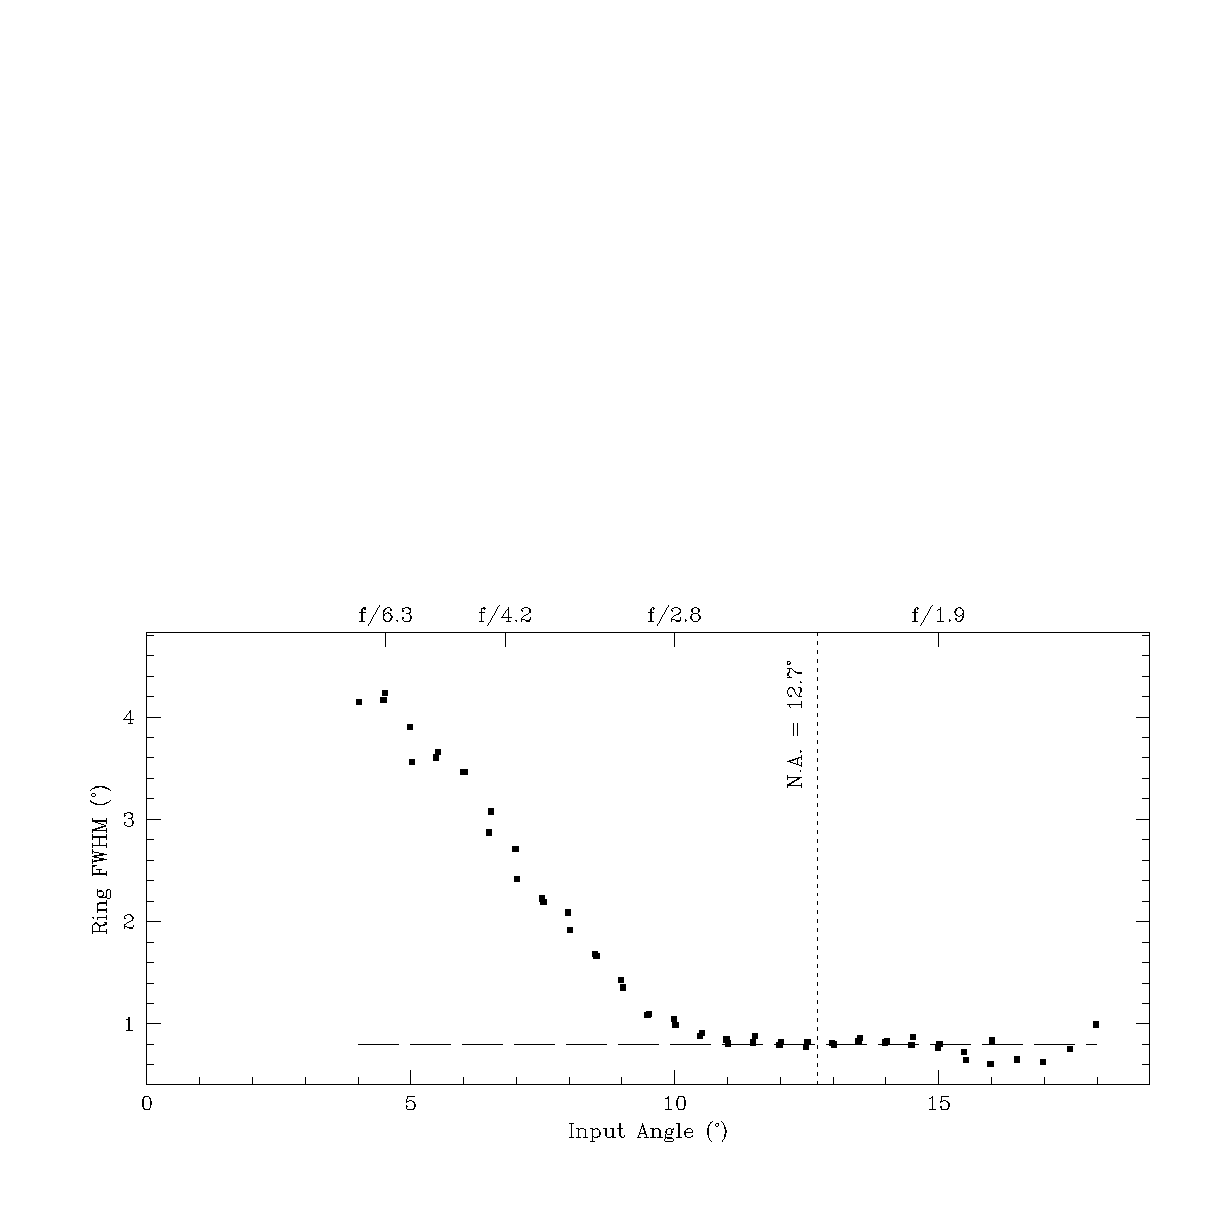
\includegraphics[width=\textwidth,trim=0 0.3in 0 3.8in,clip=true]{FRD/figs/angles.eps}
\caption[Dependence of FRD on input angle]{\fixspacing\label{fig:angle}
  Smearing due to FRD (ring width) as a function on input angle. The vertical
  dotted line marks the numerical aperture of the fiber specified by the
  vendor. The horizontal dashed line represents a best fit to the micro-bend
  model of \citet{Carrasco} over the full angular range
  of our data adopting $D=\val{1.15\times 10^{-6}}{m^{-1}}$. This value of $D$
  is constrained by a best-fit of the micro-bend model to our data in the
  range of 10 to 18 degrees.}
\end{center}
\end{figure}

Figure \ref{fig:angle} shows how the amount of ``smearing'' caused by
FRD (ring width) varies with different input beam angles. Angles below
$4^{\circ}$ are not plotted; future reports of this experiment will
measure ring widths in the regime where ring-width exceeds ring
radius.

The results in figure \ref{fig:angle} show that FRD effects are very
large at small angles, as expected, and decrease with increasing
angle until leveling out at $\sim 10^{\circ}$, which is within a few
degrees of the numerical aperture (12.7$^{\circ}$). It is possible to
extend the ring measurements to angles above the numerical
aperture. While the throughput decreases in this regime, the FRD
appears to remain fairly constant.

We have compared these trends to predictions of the micro-bend model
presented in \citet{Carrasco}.  We find a micro-bend parameter of
$D=\val{1.15\times 10^{-6}}{m^{-1}}$ provides the best fit to our data
(plotted in figure \ref{fig:angle}). This is a lower limit on the
value of $D$ for this fiber.  An upper limit on the value of $D$ comes
from matching the micro-bend model to our widest ring ($4^{\circ}$),
from which we find $D<\val{2.0\times 10^{-5}}{m^{-1}}$. For this range
of $D$, our measurements are in an angular regime where the micro-bend
model predicts a ring width nearly constant in angle. The fact that
our data show a non-constant ring-width indicates that this micro-bend
model is not a good description of the data and therefore not likely
the physical origin of FRD.

Our results are also important because they indicate just how strongly
FRD is dominated by light entering the fiber at smaller angles with
respect to the fiber optical axis. In astronomical applications,
fibers are typically fed by on-axis optical systems with central
obstructions from secondary and/or field-corrector optics. From an
entropy stand-point, i.e., information gathering-power per unit cost,
the central rays obscured are the least valuable. Consequently,
wide-field survey-telescopes \citep[e.g., SDSS, ][]{York00,Gunn06},
which are fast and have relatively large central obstructions, are
ideally suited to fiber coupling. Further analysis of data like that
in Figure 7 will allow us to quantify this statement.

\section{Summary}
\label{FRD:sec:summary}
Two experiments to 
measure the
amplitude of FRD as a function of wavelength, surface polish, 
and light-injection angle have been carried out and described.
The primary results are:
\begin{enumerate}

\item A component of FRD is attributable to the end-polish
  on fiber surfaces, however this appears to be a second-order effect
  relative to the impact of light-injection angle (beam speed) slower
  than \f3. FRD decreases with polishing down to finer grit sizes, but
  not significantly below grit-sizes of 5\mum.

\item Total throughput (light emerging at all angles) also depends on
  end-polish, with a wavelength dependence that indicates the increase
  in throughput is simply a reduction in surface-scattering.  The most
  significant gains occur for polishing that proceeds down to 5 $\mu$m
  grit, although for most astronomical applications at low
  light-levels polishing down to the finest grit is measurably
  advantageous.

\item The amount of FRD does \textbf{not} depend on wavelength, as found now
  in several experiments. This is in contrast to the predictions of micro-bend
  theory for FRD's origin \citep{Carrasco}.

\item FRD is dominated by light entering the fiber at smaller angles
  (in our case $<10^{\circ}$), as is well known. Measurements here
  allow us to quantify this statement in detail. The amplitude and
  angular dependence of FRD also do not agree with predictions from
  micro-bend theory.

\end{enumerate}

This work was supported by NSF grants ATI-0804576 and AST-1009471.

\bibliographystyle{thesis}
\bibliography{FRD}

\chapter[\GP Construction]{\GP and HexPak: A Variable-pitch, Dual-head IFU for the WIYN 3.5m Bench Spectrograph}
\label{chap:pak_build}
\epigraph{\fixspacing\emph{When the going gets weird, the weird turn
    pro}}{Raoul Duke}

% Leave space between title and quote or publication note.  This has often been
% 10cm for a quote and 8 cm for a reference, but this is really up to you.
%\vspace{8cm}

\vfill

\begin{flushright}
  \fixspacing
  \textit{A version of this chapter has previously appeared in\\
    \emph{Ground-based and Airborne Instrumentation for Astronomy IV. Proceedings of the SPIE}}\\
    \vspace{1ex}
    Wood, et. al. 2012. Volume 8446, article 84462W
\end{flushright}

%%%%%%%%%%%%%%%%%%%%%%%%%%%%%%%%%%%%%%%%%%%%%%%%%%%%%%%%%%%%% 
\begin{chabstract}
  We describe the design, construction, and expected performance of two new
  fiber integral field units (IFUs) --- HexPak and \GP --- for the WIYN 3.5m
  Telescope Nasmyth focus and Bench Spectrograph.  These are the first IFUs to
  provide formatted fiber integral field spectroscopy with simultaneous sampling
  of varying angular scales.  HexPak and \GP are in a single cable with a
  dual-head design, permitting easy switching between the two different IFU
  heads on the telescope without changing the spectrograph feed: the two heads
  feed a variable-width double-slit.  Each IFU head is comprised of a fixed
  arrangement of fibers with a range of fiber diameters.  The layout and
  diameters of the fibers within each array are scientifically-driven for
  observations of galaxies: HexPak is designed to observe face-on spiral or
  spheroidal galaxies while \GP is optimized for edge-on studies of galaxy
  disks.  HexPak is a hexagonal array of 2.9 arcsec fibers subtending a 40.9
  arcsec diameter, with a high-resolution circular core of 0.94 arcsec fibers
  subtending 6 arcsec diameter.  \GP is a 39 by 55 arcsec rectangular array
  with rows of fibers of increasing diameter from angular scales of 1.9 arcsec
  to 5.6 arcsec across the array.  The variable pitch of these IFU heads allows
  for adequate sampling of light profile gradients while maintaining the photon
  limit at different scales.
\end{chabstract}
\cleardoublepage

\section{INTRODUCTION}
\label{GPB:sec:intro}
HexPak and \GP are two new formatted fiber optic integral field units
(IFUs) for the WIYN 3.5m telescope Bench Spectrograph\footnotemark.
\footnotetext{The WIYN Observatory is a joint facility of the University of
  Wisconsin-Madison, Indiana University, Yale University, and the National
  Optical Astronomy Observatory.}  These two IFUs are unique because they are
the first formatted fiber IFUs to include multiple fiber diameters within the
same fiber head.  Including multiple fiber diameters allows each of these IFUs
to simultaneously sample different angular scales within the same observation.
The smaller fibers can gather light from higher surface brightness regions
(e.g.\ the core or midplane of a galaxy disk) while the larger fibers can
collect light from fainter, more diffuse regions (e.g.\ larger scale heights
or scale radii of a disk), thereby enabling high S/N measurements to be
obtained simultaneously at a range of spatial positions.


The two IFUs share the same cable and ``foot'' for mounting onto the WIYN
Bench Spectrograph.  Sharing the same cable minimizes the total volume
required for routing within the WIYN telescope in an already over-filled
system.  Sharing the same foot results in a unique dual-slit design, allowing
the two heads to be exchanged at the telescope without requiring changes to
the spectrograph system.  HexPak has a high-resolution core of fibers three
times smaller in diameter than the surrounding fibers.  As a hexagonal array
with a circular, high-resolution core, HexPak is tailored for studies of
radially-distributed, diffuse light sources, such as face-on galaxy disks,
spheroidal galaxies, or star clusters.  The \GP head consists of five
different fiber sizes, arranged in rows to form a gradient of fiber diameters
from one edge of the array to the other.  It is designed for integral field
spectroscopy of edge-on galaxies, making it well-suited for studying
extra-planar gas and stars in spiral galaxy disks.


Including multiple fiber diameters comes at a cost, however.  In the case
where the system spectral resolution is limited by the slit width, this will
result in a varying spectral resolution, inversely proportional to the fiber
diameter.  In this case the maximum resolution will change by a factor of 3
for \GP and 3.1 for HexPak, increasing from the largest to the smallest
fibers.  However, the smallest reimaged fiber sizes will have contributions
from optical aberrations from the spectrograph. As a result, we expect the
achievable resolution to increase only by a factor of 2--2.5 for HexPak.

The science impact of changing spectral resolution depends on the specific
application.  For example, the velocity dispersion of stars is expected to
increase with scale height above the disk midplane in edge-on disk galaxies.
For the study of stellar velocity dispersions in spheroidal or face-on disk
galaxies, as another example, it would be advantageous to \emph{increase}
spectral resolution with radius, since systems become dynamically colder
moving outward.  This is opposite what these instruments deliver.  On the
other hand, at lower surface brightness the limits of S/N prevent useful
information from being obtained at high spectral resolution, and in this sense
these instruments provide a practical balance between signal and resolution.
As we describe below, ample sky fibers are included for all fiber sizes to
ensure excellent sky subtraction.

This instrument follows in the legacy of the excellent WIYN fiber IFUs
DensePak \citep{Barden98} and SparsePak \citep{Bershady04,Bershady05}.  The
primary impetus behind this project was the increased throughput and image
quality of the newly redesigned WIYN Bench Spectrograph
\citep{Barden94,Bershady08,Knezek10}.  In the process an opportunity arose to
rebuild the decommissioned DensePak IFU.  The fiber from DensePak is being
reused for the larger fibers in the new HexPak array, and most of the hardware
in the cable ``foot'' housing that terminates the cable in the spectrograph
room at WIYN is reused from the DensePak cable.  HexPak contains additional
fibers that were newly purchased for this project.  \GP is made entirely using
new fiber.  Additionally, all the cabling and head mount hardware is newly
constructed.


In \S\ref{GPB:sec:design} we detail the key science drivers that served as a
design target for the instrument, as well as describe the design challenges
inherent in the design of formatted IFUs with multiple fiber diameters.  We
detail the construction process in \S\ref{GPB:sec:construction} and summarize the
project in \S\ref{GPB:sec:conclusion}.

%%%%%%%%%%%%%%%%%%%%%%%%%%%%%%%%%%%%%%%%%%%%%%%%%%%%%%%%%%%%%
\section{DESIGN} 
\label{GPB:sec:design}
%%%%%%%%%%%%%%%%%%%%%%%%%%%%%%%%%%%%%%%%%%%%%%%%%%%%%%%%%%%%%
\subsection{Science drivers} 
\label{GPBsub:sec:scidri}
These IFUs are designed for studying nearby galactic stellar populations, the
ISM of other galaxies, and stellar and gas kinematics of nearby galaxies.
Science drivers that influenced the design of the IFUs include: probing the
vertical structure of spiral disks using stellar and gas kinematic tracers;
studying the kinematics and abundances of diffuse ionized gas in edge-on and
face-on spiral galaxies; understanding the origin of winds in starburst
galaxies; measuring the rate of galactic outflows in normal spirals; and
connecting the properties of galaxy cores to the secular evolution of their
parent galaxies for E+A galaxies, QSO/AGN hosts, and pseudo-bulges.



%%%%%%%%%%%%%%%%%%%%%%%%%%%%%%%%%%%%%%%%%%%%%%%%%%%%%%%%%%%%%
\subsection{Head design} 
\label{GPBsub:sec:heads}
The primary limitations on the overall head size result from technical
limitations in the telescope and spectrograph system.  The maximum number of
fibers is limited simply by the maximum allowable slit length.  The overall
field of view is limited by the IFU mount on the telescope.  The IFU heads
mount into the WIYN Fiber-Optic Echelle (WIFOE) port on the telescope.  The
WIFOE port limits the overall head mount to a 1in circular diameter.
Accounting for mounting hardware, this limits the overall physical IFU head
size to approximately a square 0.5in$\times$0.5in, corresponding to a maximum
field of view (FOV) of $119\arcsec\times119\arcsec$ at the WIYN plate scale of
9.\farcs374/mm.  Packing fibers and head mount fixturing make the usable FOV
somewhat smaller than this, as shown later.


Each IFU head design presented a unique challenge for packing the fibers
together to form the heads.  The main problem we needed to overcome was one of
``circle packing'': what is the best way to arrange the fibers (represented as
circles as viewed along the optical axis of the system) so that we maximize
the focal plane filling factor in a compact region while achieving our target
scientific capability?  To our advantage, the problem of circle packing has
been relatively well-studied in the field of geometry.  For a single diameter,
the highest density packing arrangement is a hexagonal lattice arrangement as
used in both DensePak and the SparsePak array on WIYN, which results in a
packing density of $\pi/\sqrt{12} \approx 0.907$ \citep{Steinhaus99}.  Circle
packing becomes markedly more difficult when including more than one circle
diameter in the packing, as each of these new IFU heads does.  Our conceptual
goal for these IFUs was to enable the simultaneous sampling of varying surface
brightness levels in the same IFU observation.  To that end, the challenges of
circle packing were central to our ability to design these IFU heads in a way
that achieved our scientific goals yet were within our ability to fabricate.
In the following sections we describe the challenges we have overcome to
develop scientifically-useful head designs that were also feasible to
construct.


\subsubsection{HexPak}
\label{GPBsubsub:sec:hexhead}

\begin{figure}
    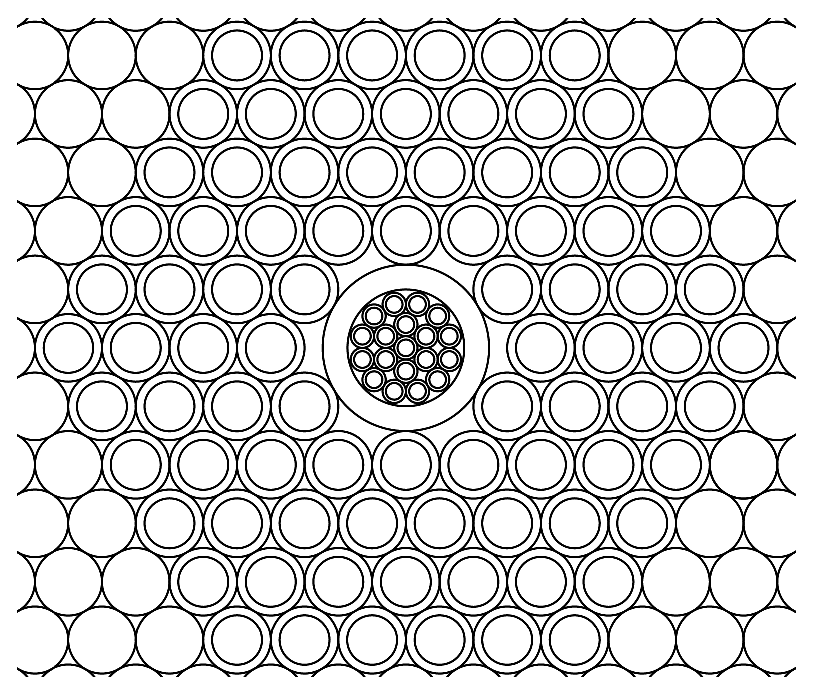
\includegraphics[width=0.48\textwidth]{Pak_build/figs/hexpak_zoom}
    \hfill
    \includegraphics[width=0.48\textwidth]{Pak_build/figs/19fibers}
    \vspace{1.5mm}
    \caption[HexPak Science Fibers]{\fixspacing \emph{Left:} Detail of the
      HexPak science fibers.  Fiber core regions are not shown for packing
      fibers.  The region depicted is approximately 0.18in$\times$0.15in
      centered on the hexagon.  \emph{Right:} Prototype of the HexPak core
      packing.  The fibers and capillary were glued into a 0.25in brass
      ferrule and ground to an even length in order to observe the quality of
      the packing.  This face has not been well-polished and does not
      represent our final target level of surface polish.
    \label{fig:hex_head}}
\end{figure}


The HexPak IFU head is designed to study objects with radial surface
brightness profiles (e.g.\ face-on galaxy disks, spheroidal galaxies).  As the
name suggests, HexPak is a hexagonal fiber array, based on a hexagonal lattice
arrangement.  As a result, the larger-diameter HexPak fibers are arranged in
the most compact manner possible.  The fiber diameter for the hexagonal region
was set by the diameter of the pre-existing DensePak fibers.  These fibers
have core diameters of 310$\mu$m and full outer diameters measured to be
$405\mu$m.  At the plate scale of the WIYN focal plane the cores of these
fibers span 2.\farcs8\ on the sky.  The design goal for the HexPak head was to
have a hexagonal region of fibers in an annulus around a high-spatial
resolution fiber core, necessitating two different fiber diameters.  There are
only nine possible compact\footnotemark\ packings of two circle diameters in a
plane \citep{Kennedy06}.  \footnotetext{A packing is ``compact'' if, for every
  circle \emph{C} that is tangent to a series of circles
  \emph{C}$_1$,\emph{C}$_2$,\dots,\emph{C}$_n$, circle \emph{C}$_i$ is tangent
  to circle \emph{C}$_{i+1}$ for $i = 1,2,\dots,n$.}  Of these, only one is
particularly relevant to the science goals of HexPak.  This packing involves
replacing one larger circle with an array of seven smaller circles (with a
diameter ratio of $\sim$0.386) while retaining the hexagonal lattice
arrangement of the other large circles (see Figure~1.e in
Ref.~\citenum{Kennedy06}).


The main flaw in this design as it pertains to our design goals is that the
seven smaller circles \emph{must} be surrounded by larger circles to maintain
a compact packing.  Stated differently, this arrangement dictates that the
high-resolution core of HexPak be no larger than the diameter of one large
fiber.  The reason behind this is that the largest radius occupied by the
seven smaller fibers is larger than the radius of the one fiber which was
removed.  Adjacent packings of seven small fibers would therefore overlap each
other.  This means that this packing arrangement would allow for higher
spatial sampling of no larger than a 2.\farcs8\ diameter region, but we felt a
larger region would more closely meet our science goals.  In order to achieve
a larger high-resolution core, we realized that this particular compact
packing can be reversed by instead replacing seven circles with one larger
circle.  This reversal ultimately led to the final design.


For the final HexPak head design we have replaced the central seven
2.\farcs8\ fibers in the hexagon with a glass capillary tube.  The outer
diameter of this tube is such that it packs compactly to the surrounding
fibers, and the inner diameter of the tube leaves a large, circular profile in
which we can pack small fibers.  Our final task was to determine how to
densely pack a moderate number of fibers inside this new circular aperture.
In order to determine an efficient packing within this aperture, we once again
turned to the study of circle packing.  A sub-field of circle packing
investigates the most efficient methods for packing circles of a given
diameter into one circle of a larger diameter.  Ref.~\citenum{Kravitz67}
presents empirically-derived optimal packings of circles into a circular
container.  For a diameter ratio of $\sim$0.206, it is possible to pack 19
small circles into one larger circle.  This final design of all the HexPak
object fibers can be seen on the left in Figure~\ref{fig:hex_head}.


It was prohibitively expensive to fabricate a form for a custom diameter
capillary draw just a few inches in length, so in practice our chosen diameter
(and the diameters of the fibers in the core) was limited to stock sizes.  In
the case of HexPak, our chosen glass capillary was purchased from Polymicro
Technologies\footnotemark\ and has a specified inner diameter of 750$\mu$m.
\footnotetext{Polymicro Technologies, 18019 N.\ 25th Avenue, Phoenix, AZ
  85023--1200, (602) 375--4100} This capillary inside diameter corresponds to
a core fiber outer diameter of about 154$\mu$m.  The closest stock fiber outer
diameter from Polymicro was 140$\mu$m (100$\mu$m or 0.\farcs94 core diameter),
resulting in the final design of 19 0.\farcs94\ fibers packed in the center of
the hexagon.  One sacrifice we make in using stock sizes is that there is a
2--3\arcsec\ gap between the core fibers and the larger fibers in the
hexagonal region.  The necessary outer diameter to fill the space of seven
405$\mu$m OD fibers is 1,050$\mu$m, but this capillary has an outer diameter
of 850$\mu$m.  This amount of undersizing is problematic for the packing
arrangement.  We manually thickened the pieces of capillary used in the head
by applying thin coatings of spray paint to the tubes until we reached the
desired diameter.


\begin{figure}[t]
    \centering
    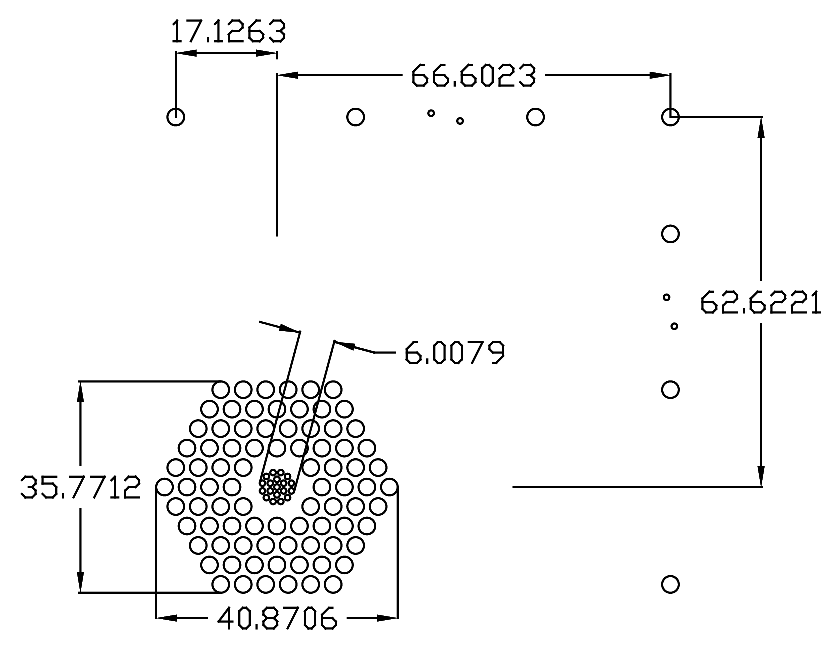
\includegraphics[width=.55\textwidth]{Pak_build/figs/hexpak}
    \hfill
    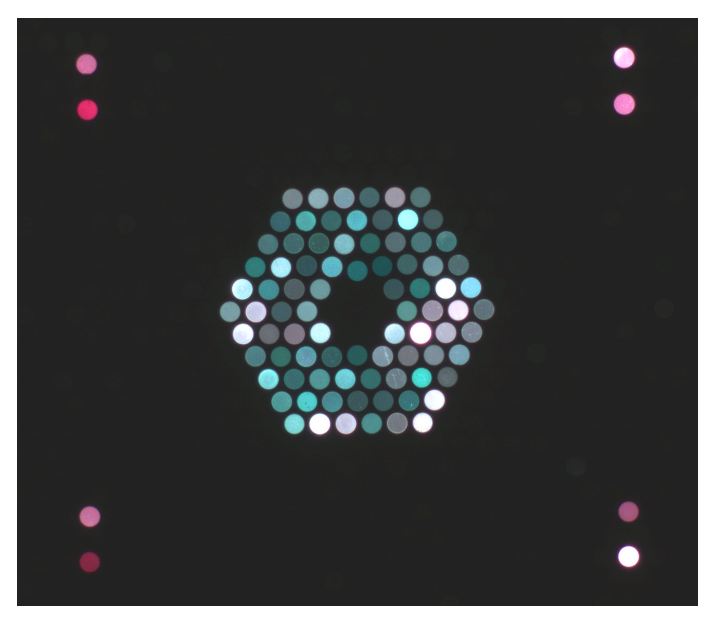
\includegraphics[width=.42\textwidth]{Pak_build/figs/hex_proto}
    \vspace{1.5mm}
    \caption[HexPak Design]{\fixspacing \emph{Left:} Head design for the
      HexPak IFU.  All displayed values are in units of arcseconds.  The two
      different fiber diameters are 2.\farcs8 and 0.\farcs94 on the sky.  Only
      the active fiber core regions are shown.  \emph{Right:} An image of an
      early prototype of the HexPak head design.  The center of the hexagonal
      region contains a hypodermic needle as a placeholder for the capillary
      with small fibers.  No small fibers are in the hypodermic shown here.
      The ends of the fibers were colored with marker to easily differentiate
      object fibers (green) from sky fibers (red).
    \label{fig:hexpak}}
\end{figure}


Although the results from Ref.~\citenum{Kravitz67} are empirical (and
therefore may not be compact) and our chosen fibers are slightly undersized,
the amount of extra space in the packing arrangement is at an appropriate
level to allow for mechanical tolerances.  We have successfully assembled two
prototypes of this packing and have high confidence that this will be viable
in the final head assembly.  The right side of
Figure~\ref{fig:hex_head} shows one of these prototypes after being
glued and roughly polished.


Our final head design is shown in Figure~\ref{fig:hexpak}.  The array design
has 114 total fibers.  Of these, the main science fiber region consists of 84
fibers with 2.\farcs8\ diameters contained within the outer hexagonal region
and 19 fibers with 0.\farcs94\ diameters spanning the central
6\arcsec\ diameter of the hexagon.  The capillary tube housing the
0.\farcs94\ fibers creates an annular gap 2--3\arcsec in radius between the
core fibers and the outer hexagonal region.  The array also has 11 total sky
fibers, seven with 2.\farcs8\ diameters and four with 0.\farcs94\ diameters.
The sky fibers are placed along the edges of the array opposite the science
fibers to maximize the separation between the object and sky sampling regions.
The sky fibers lie between 45\arcsec\ and 75\arcsec\ from the \emph{edge} of
the hexagon.  The HexPak head design employs nearly 1,000 short (3in) packing
fibers to fill the space in between the science fibers and the sky fibers,
similar to the scheme used for SparsePak.  The packing fibers also create a
roughly rectangular exterior head profile.  An early prototype of the HexPak
design is also shown in Figure~\ref{fig:hexpak}.  This prototype shows an
earlier revision in sky fiber arrangement and contains no small fibers in the
core of the array.


Ref.~\citenum{Bershady04} found that focal ratio
degradation\footnotemark\ (FRD) increases at the edge of the SparsePak array.
\footnotetext{Focal ratio degradation is a decrease in focal ratio of a beam
  as it passes through a fiber.}  They suggest several possible causes,
including stress incurred when releasing the head from its mold and pressure
introduced by the head-mount clamp.  Regardless of the cause, they recommend
leaving at least a 1.2mm buffer region at the outside of the head in order to
protect the active fibers from these potential stresses.  The ``packing
fiber'' buffer in the HexPak head is four large fibers, or about 1.6mm, which
we expect will alleviate FRD increases at the edge of the array.


\subsubsection{\GP}
\label{GPBsubsub:sec:gradhead}

\begin{figure}[t]
    \centering
    \begin{minipage}[c]{0.5\textwidth}
        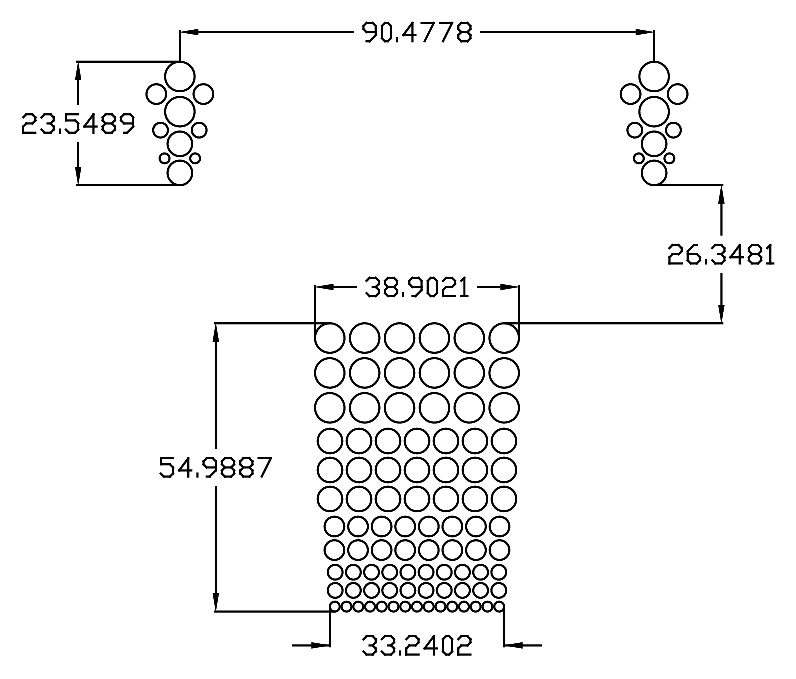
\includegraphics[width=0.95\textwidth]{Pak_build/figs/gradpak}
    \end{minipage}
    \hfill
    \begin{minipage}[c]{0.41\textwidth}
        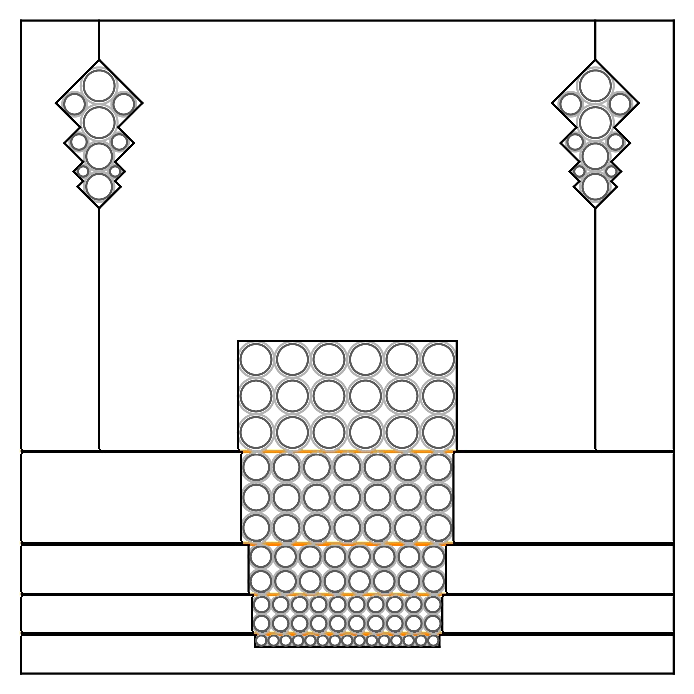
\includegraphics[width=0.95\textwidth]{Pak_build/figs/gradpak_zoom}
    \end{minipage}
    \vspace{1.5mm}
    \caption[\GP Layout]{\fixspacing \emph{Left:} Fiber layout for the \GP
      IFU.  All displayed values are in units of arcseconds.  The different
      fiber diameters are 1.\farcs9, 2.\farcs8, 3.\farcs7, 4.\farcs7, and
      5.\farcs6 on the sky.  Only the active fiber core regions are shown.
      \emph{Right:} Detail of the \GP head mount.  The darker gray circles
      are the active fiber cores, the lighter gray circles are the full
      O.D.\ of the fibers, and the orange lines represent $25\mu$m-thick
      plastic dividing layers.  The full exterior profile measures
      0.5in$\times$0.5in.
    \label{fig:gradpak}}
\end{figure}


\GP is designed to study objects that exhibit linear gradients in surface
brightness (e.g.\ edge-on galaxy disks, linear outflows).  Therefore, the
desired fiber arrangement in the head is linear rather than approximately
circular as it is in HexPak.  The design goal was to approximate layered
pseudo-slits of increasing slit width, accomplished by using stacked rows of
fiber, with fiber diameters increasing between rows.  There is no compact
packing of two different circle diameters that allows for each fiber size to
be arranged into linear, contiguous rows.  Circle packing theory did not show
obvious solutions for this problem, so we settled on a design that uses five
physically separated fiber regions, each containing only a single fiber
diameter.  This design is shown on the left in Figure~\ref{fig:gradpak}.  Our
final design includes a total of 110 fibers composed of five different fiber
core diameters: 200$\mu$m, 300$\mu$m, 400$\mu$m, 500$\mu$m, and 600$\mu$m.
Respectively, these fibers span angular diameters of 1.\farcs9, 2.\farcs8,
3.\farcs7, 4.\farcs7, and 5.\farcs6\ at the WIYN focal plane.  In order to
successfully accommodate five different fiber diameters within the same
packing arrangement, we have designed a layered head mount.


This head mount fixturing represents one of the largest engineering challenges
we have overcome.  In order to get each row of fibers to remain parallel to
each other, fibers of different diameters could not touch.  This is a result
of there being no compact packing of two different fiber diameters that allows
for parallel rows.  This meant that it would be impossible to use short
packing fibers in the \GP head.  After numerous iterations, we ultimately
designed a layered head mount that is assembled in stages, one fiber-diameter
region at a time.  The final head mount design can be seen on the right in
Figure~\ref{fig:gradpak}.  Each set of fibers of a given diameter is contained
by aluminum walls, precisely machined to the height of each fiber region.  The
head is then assembled by layering subsequent stacks of these segments on top
of one another.  All of the parts of the fixture are held together as an
assembly using small dowel pins that run the full height and width of the
assembly.  The main cavity was cut out as an assembly using a wire electric
discharge machining (EDM) process to ensure the best possible alignment
between adjacent fiber regions.  The \GP head block cavity was cut using a
0.004in diameter wire, allowing for a minimum corner radius of 0.002in
(50$\mu$m), small enough to ensure the smallest fibers fit into place.

The dimensions of the entire head block are 0.5in$\times$0.5in.  Each region
of fibers containing a single fiber diameter is separated from its neighbors
by a thin layer of plastic shim stock 0.001in (25.4$\mu$m) thick.  Although
this adds a gap between each region of fibers, the on-sky angular size of the
plastic layer is very small (0.\farcs24), which we deemed acceptable.  We have
successfully designed and assembled two prototype \GP head assemblies and
we are confident that this design is feasible.


The resulting array design consists of five stacked blocks of fibers arranged
into one or more rows, with the fiber core diameter increasing from 200$\mu$m
to 600$\mu$m between each block of fibers.  The entire block of science fibers
includes 90 fibers and covers an area on the sky roughly
35\arcsec$\times$55\arcsec.  The array also has two regions of sky fibers for
simultaneous sky measurements.  Each sky fiber region contains two fibers of
each fiber diameter included in the science fiber region.  The fibers in
\GP are arranged in a square lattice rather than in a hexagonal lattice,
reducing the effective filling factor within each fiber region.  This yields a
packing density of only $\pi/4 \approx 0.785$.  The advantage of this
arrangement is that the pseudo-slits within each region are vertically aligned
and are offset only in one dimension on the sky.


Since the entire \GP head mount assembly is composed of aluminum parts, no
short packing fibers are used in its design.  The design does, however, place
active fibers within 1.2mm of the edge of the head, inside the prescribed
minimum buffer distance.  However, we believe FRD edge effects should be
negligible due to the use of a stronger buffer material (aluminum in this
case) and the fact that at no point during assembly is any part of the \GP
head released from a mold.


%%%%%%%%%%%%%%%%%%%%%%%%%%%%%%%%%%%%%%%%%%%%%%%%%%%%%%%%%%%%%
\subsection{Slit design} 
\label{GPBsub:sec:slit}

\GP and HexPak both terminate in the same ``foot'' housing in a dual-slit
configuration.  The slit block uses a custom design that modified the
SparsePak slit block design.  The slit block assembly is made from two
separate aluminum plates, each specifically designed to create a pseudo-slit
for one of the IFUs.  Each pseudo-slit was created by cutting `v'-grooves into
the slit block.  The groove size, placement, and spacing is designed to match
the varying number and sizes of fibers in each IFU pseudo-slit.  A schematic
of the slit block assembly is shown in Figure~\ref{fig:slit}.  For mechanical
reasons, the fibers are aligned to be tangent to the optical centerline of the
slit, rather than being aligned by their centers.  The `v'-grooves were
precision-cut into the slit block using a wire EDM process like that used for
the \GP head mount fiber cavity, but with a smaller $0.002$in diameter
wire, resulting in a minimum corner radius of approximately $0.001$in
($25\mu$m).  This radius is smaller than the smallest fiber outer radius
(measured to be about 71$\mu$m) ensuring that even the smallest fibers will
sit nicely into the grooves.


We have set the fiber core edge-to-edge spacing at $291\mu$m to minimize
cross-talk while maximizing the number of fibers in the slit.
Ref.~\citenum{Bershady04} found that 400$\mu$m was the ideal edge-to-edge
spacing of fiber cores in the slit in terms of the trade-off between
cross-talk and packing density (i.e.\ total number of fibers).  However, this
determination was made using the old Bench Spectrograph system which was
upgraded in 2008 \citep{Bershady08}.  With improved image quality and detector
sampling as a result of the upgrade, we estimate we can reduce the fiber
spacing by $\sim25\%$ without introducing significant amounts of cross-talk
between fiber channels.


The fiber arrangements in the slit are informed by their locations within the
head design.  In HexPak, the hexagonal region is divided into six equal
wedges, each containing 14 fibers.  The fibers within each wedge are located
in the same region of the slit, with fibers near the core of the array being
located in the center of the slit segment.  Each wedge section in the slit is
separated from the adjacent wedge sections by a sky fiber, allowing sky
sampling across the entire slit length.  Three wedges and associated sky
fibers are located on each end of the slit, separated by all of the 0.\farcs94
fibers.  The 0.\farcs94 fibers are located in the center of the slit, with the
associated 0.\farcs94 sky fibers being located on either side of the
0.\farcs94 object fibers.  The \GP slit is sorted by fiber diameter.
Within each diameter region, each fiber row in the head is placed contiguously
in the slit, with sky fibers evenly distributed as separators between rows.


We also slightly modified the standard Bench Upgrade design for the ``toes''
of the cable in order to negate vignetting of the light exiting the fiber
slit.  The toes house the slit block and have open chambers for inserting
blocking filters, slit masks, and a back-illumination mirror.  These chambers
each have an aperture through which the exit beam must pass in order to reach
the spectrograph collimator.  We performed a vignetting analysis to determine
the maximum fiber slit width and slit length that could pass unvignetted
through the toes.  Ref.~\citenum{Bershady04} shows that, due to FRD, 99\% of
the energy in an \f6.3 input beam (the WIYN focal ratio) exiting the fibers is
contained within an \f4 output beam.  Therefore, as long as an \f4 beam could
pass through the toes without being blocked, we could consider light losses
from the toes to be negligible.  The SparsePak design for the toes allowed for
a maximum slit length of 79.8mm under this vignetting requirement.  This
number informed the fiber-to-fiber spacing for our final slit design,
resulting in an overall slit length of 76.6mm.  The maximum allowable slit
width for an \f4 beam was 1.23mm, or a $615\mu$m beam displacement from slit
center.  Our largest fiber has a $600\mu$m core diameter with approximately
$55\mu$m of clading and buffer in radius.  Each half of the slit block also
has a $25\mu$m plastic divider at slit center, a requirement of our slit block
construction process.  In total, the maximum beam displacement from slit
center is about $680\mu$m, too large for the standard design for the toes.  As
a result, we modified the design and increased the width of one critical
aperture in the toes such that the maximum allowable displacement from slit
center is $927\mu$m.


\begin{figure}[t]
    \centering
    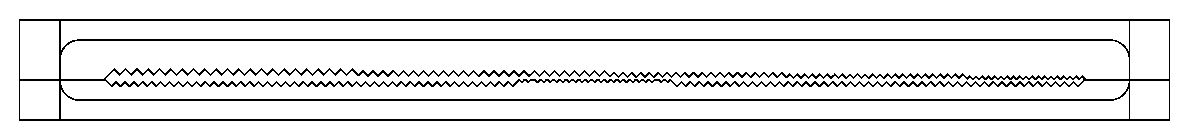
\includegraphics[width=\textwidth]{Pak_build/figs/slit}\\
    \vspace{2pt}
    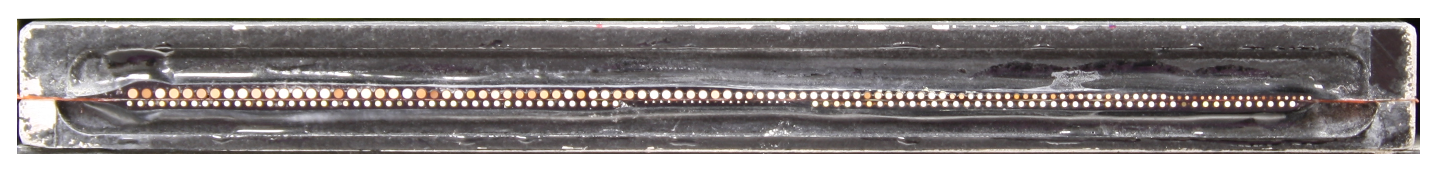
\includegraphics[width=\textwidth]{Pak_build/figs/slit_img}
    \caption[HexPak/\GP slit]{\fixspacing \emph{Top:} A schematic view of the
      slit block without fibers.  Both halves of the slit block assembly are
      shown.  The bottom set of grooves is the HexPak slit and the upper set
      of grooves is the \GP slit.  \emph{Bottom:} An image of the slit
      face in its current state.  The top row of fibers are \GP, arranged
      by decreasing diameters.  The bottom row of fibers are HexPak, with the
      0.\farcs94 fibers situated between the 2.\farcs8 fibers.  Brightness
      differences between fibers are largely due to surface irregularities in
      the unpolished head end.  Color differences are simply due to some
      fibers pointing at different parts of the lab.  The two 0.001in-thick
      plastic shim stock dividers are seen as a thin orange line separating
      the two slits.  The shown view spans 3.562in$\times$0.312in.
    \label{fig:slit}}
\end{figure}


%%%%%%%%%%%%%%%%%%%%%%%%%%%%%%%%%%%%%%%%%%%%%%%%%%%%%%%%%%%%%
\section{CONSTRUCTION AND STATUS} 
\label{GPB:sec:construction}

The design and construction of the SparsePak cable served as the starting
point for this instrument.  Technical details of SparsePak fabrication are
available in the Appendix section of Ref.~\citenum{Bershady04}.  In this
section we focus primarily on detailing the important features unique to this
instrument and noting significant departures from the SparsePak design.


At the present time, construction is complete on all cabling and the entire
spectrograph feed assembly (the foot).  Polishing of the fiber slit is nearly
complete, and final gluing and polishing of the IFU heads are scheduled to
conclude in June--August 2012.

\subsection{Fiber optics}
\label{GPBsub:sec:fibers}
The 91 2.\farcs8\ fibers that compose the hexagonal region and its associated
sky fibers are re-purposed from the DensePak IFU.  They have a specified
active core diameter of $310\mu$m and a measured total O.D.\ (including
cladding and buffer) of approximately $405\mu$m.  Ref.~\citenum{Barden98}
states that the DensePak fibers are similar to the Hydra FIP-type
``red-optimized'' fibers.  The 23 0.\farcs94\ fibers forming the
high-resolution core and associated sky fibers were purchased new from
Polymicro Technologies.  These new fibers are FBP-type broad-spectrum optical
fiber with excellent throughput for optical wavelengths.  The fibers have
silica cores with silica cladding and are designed to have excellent
throughput across the visible spectral window and into the near-infrared.  The
diameter specification (given as core:clad:buffer, in microns) is 100:120:140.
This new fiber is very similar to the fiber used in SparsePak and therefore we
expect similar throughput performance from the core HexPak fibers.

Throughput testing for SparsePak showed a roughly 20\% improvement in
throughput compared to the DensePak fibers, after accounting for differences
in fiber diameter and collected solid angle \citep{Bershady05}.  However, most
of the light loss in the DensePak cable was likely due to vignetting in the
original design of the fiber cable toes, before the Bench Upgrade.  With our
modified version of the standard Bench Upgrade toes, we expect these fibers to
have comparable performance to the SparsePak fibers in the red ($>4000$\AA;
the FBP-type fibers have better transmission properties below
4000\AA\ compared to the FIP-type fibers).

The \GP IFU consists entirely of new FBP-type broad-spectrum optical fiber
from Polymicro Technologies.  The fibers have specified diameters (given as
core:clad:buffer, in microns) of 200:220:240, 300:330:370, 400:440:480,
500:550:590, and 600:660:710.  This fiber is very similar to the fiber used in
SparsePak and therefore we expect similar throughput performance from all the
\GP fibers.


\subsection{Cabling}
\label{GPBsub:sec:cabling}
Each fiber is individually housed in a PTFE tube for protection and strain
relief.  The PTFE tubes for the $310\mu$m HexPak fibers were also re-used from
the DensePak cable.  All of the newly-purchased fiber is housed in new PTFE
tubing from Zeus, Inc\footnotemark.  \footnotetext{Zeus, Inc., 3737 Industrial
  Blvd., Orangeburg, SC 29118, (800) 526--3842} As a design decision to reduce
the radial cable size, the new PTFE tubes have ``light-weight wall''
thicknesses (0.006in in radius).  This has proven troublesome due to the
relative lack of radial strength and rigidity in the wall compared to
thicker-walled tubing.  The very thin walls of these tubes are prone to
kinking which threatens the integrity of the fibers they serve to protect.  We
recommend, at minimum, ``thin wall'' PTFE tubes ($\gtrsim$0.01in).


The PTFE tubes terminate at each end of the cable in metal shear clamps.  The
foot-end shear clamp contains an array of approximately $9\times27$ holes in a
three-element aluminum clamp.  The elongated design of this clamp serves to
transform the circular bundle of fibers into a rectangular shape approximating
the slit arrangement.  The head-end shear clamps are a similar three-element
design and function in a similar fashion to the foot shear clamp.  The hole
pattern in the head end shear clamps is roughly hexagonal in order to
accommodate the circular fiber bundle and to approximate the fiber layout of
the HexPak head.


The fibers and their PTFE tubes are encased in 75 feet of flexible metal
conduit.  The conduit housing the shared length of the cable consists of
approximately 57 feet of 2in ID IE30 and IE50\footnotemark\ interlocking
stainless steel exhaust hose.  \footnotetext{Penflex, Corp., 105B Industrial
  Drive, Gilbertsville, PA 19525, (800) 232--3539} This conduit retains
flexibility for handling while providing strength and durability for the
length of cable that will be enclosed within the telescope structure.


The remaining 18 feet of the cable is housed in two separate lengths of 1.25in
ID flexible aluminum standard electrical conduit.  Each length contains the
remaining length of fiber for one of the IFU heads.  The lightweight
construction and smaller diameter of this conduit allows for ease of handling
for mounting the IFU heads into the telescope's Nasmyth port.  These two
lengths of conduit are completely covered in polyolefin and PVC heat-shrink
tubing for additional rigidity and abrasion resistance.  The smaller lengths
of conduit are joined to the larger, stainless steel conduit through a
custom-built merge collector from the automotive industry\footnotemark.
\footnotetext{Specialty Design Products, Inc., 11252 Sunco Drive, Rancho
  Cordova, CA 95742, (888) 778--3312}


The conduit for each IFU head contains two custom-designed low-profile
rotation couplers.  Each coupler has $180^{\circ}$ of rotation about the
optical axis, allowing each IFU head to rotate a full $360^{\circ}$ with the
telescope instrument port rotator.  The two rotation couplers are spaced
approximately $12$in apart along the cable to ensure that the full rotation is
distributed along a sufficient length to avoid fiber stress.


\subsection{Fiber slit}
\label{GPBsub:sec:slitconstruct}
For gluing the fiber ends into the slit grooves, we fabricated custom metal
fixturing to bend the fibers 90$^{\circ}$ in the foot and hold them with
clearance to mount the slit blocks.  We used EPO-TEK\footnotemark\ 354
heat-curing optical epoxy to bond the fiber ends to the slit block.
\footnotetext{Epoxy Technology, Inc., 14 Fortune Drive, Billerica, MA 01821,
  (978) 667--3805} The gluing fixture held each fiber in its respective slit
position and allowed us to seat all the fibers simultaneously.  We used a thin
sheet of plastic to cover the exposed fiber and epoxy and held the fibers in
place using an aluminum pressing block while the epoxy cured.  We glued each
slit block separately and then constructed the final assembly from the two
completed halves.  The two halves are pinned together to ensure accurate,
repeatable positioning between the two slit halves.

\subsection{Fiber heads}
\label{subsec:headconstruct}
As tested with SparsePak and our HexPak and \GP test head assemblies, we
will use the same EPO-TEK 354 heat curing epoxy for assembling the IFU heads.
The HexPak head is assembled one row of fibers at a time, using short packing
fibers to fill in the spaces around the active fibers.  The 0.\farcs94\ fibers
are pre-assembled into their capillary tubes and then placed into the final
assembly during the gluing process.  For constructing the HexPak head, we
follow a design and process used for SparsePak, based on a concept from
S.\ Barden (\emph{private communication}).  We will assemble the fibers in a
micrometer-driven vice with the vice channel width set precisely to the width
of the head.  We will then use a precisely-machined tamping tool, just
slightly narrower than the width of the head, to pack the fibers into the
channel mold.  The mold and the tamping tool are sprayed with a PTFE mold
release\footnotemark[1]\ prior to gluing.  \footnotetext[1]{Miller--Stephenson
  Chemical Company, Inc., 55 Backus Ave., Danbury, CT 06810, (203) 743--4447}


The \GP head is assembled one fiber region at a time, with all fibers of a
single diameter being assembled at the same time.  The assembly is cured after
each additional region is assembled.  In contrast to the HexPak construction,
no vice is used for \GP.  The head mount parts are machined to the precise
cavity width to hold the fibers for each region, requiring only a pressing
plate to ensure the fibers remain seated in the cavity while curing.  The
pressing plate is coated in PTFE mold release as a precaution and separated
entirely from the epoxy by the plastic dividing layers, so at no point are the
fibers released from a cured mold.  This should alleviate any additional FRD
introduced through fiber stresses when releasing the mold, as seen in
SparsePak.


%%%%%%%%%%%%%%%%%%%%%%%%%%%%%%%%%%%%%%%%%%%%%%%%%%%%%%%%%%%%%
\subsection{Polishing}
\label{subsec:polishing}
We will polish the optical surfaces of the fiber slit and each of the fiber
heads in order to minimize light losses and FRD as the light passes through
the cable.  We are using an UltraPol\footnotemark[2]\ 1200 model lapping
machine with 8in diameter silicon carbide and aluminum oxide lapping disks.
\footnotetext[2]{ULTRA TEC Manufacturing, Inc., 1025 E.\ Chestnut Avenue,
  Santa Ana, CA 92701, (877) 542--0609} The lapping disks span a range of grit
sizes, starting from $70\mu$m for the grinding phase to $0.3\mu$m for the
final polishing phase.  Our laboratory testing shows that FRD is minimized for
surface roughnesses $<5\mu$m.  Our target surface roughness is $<0.5\mu$m.
See Eigenbrot et al.\ in these proceedings for a full description of our FRD
and surface polish testing.  At the time of this writing, the entirety of the
slit was polished at a 5$\mu$m level and ready to proceed to 1$\mu$m grit
disks, followed by 0.3$\mu$m grit.  An image of the slit in this state is
shown in Figure~\ref{fig:slit}.


%%%%%%%%%%%%%%%%%%%%%%%%%%%%%%%%%%%%%%%%%%%%%%%%%%%%%%%%%%%%%
\section{SUMMARY} 
\label{GPB:sec:conclusion}

We are in the final construction phase of two new fiber optic IFUs, \GP
and HexPak.  These IFUs will be the first formatted fiber IFUs to utilize
multiple fiber diameters within the same IFU head.  By including multiple
fiber diameters these IFUs will greatly expand the spectroscopic capabilities
of the WIYN 3.5m telescope, providing the ability to sample varying spatial
scales within the same observation with the highly versatile Bench
Spectrograph.  This will enable observations simultaneously spanning a wide
range in surface brightness to be optimized for the photon limit at spectral
resolutions between 1000 $< \lambda/\Delta\lambda <$ 30,000.


HexPak is designed to observe axi-symmetric surface brightness profiles with a
$36\arcsec\times41\arcsec$ hexagonal region sampled by 2.\farcs8\ fibers and a
6\arcsec diameter high-resolution core sampled by 0.\farcs94\ fibers.  \GP
is optimized for linear surface brightness gradients, with a stacked
pseudo-slit design spanning $39\arcsec\times55\arcsec$ using fibers ranging
from 1.\farcs9\ to 5.\farcs6\ in diameter.  Each of these IFUs presented
unique challenges for successfully incorporating multiple fiber diameters
within the same fiber head.  We have described two methods for overcoming
these challenges, one for radial arrangements of fibers and one for linear
arrangements.  Our solutions optimize the packing fraction of science fibers
while also achieving regular and precise placement and configuration of fibers
within each IFU.

\bibliographystyle{thesis}
\bibliography{Pak_build}

%\chapter[Using \GP]{Observing NGC 891 with \GP: Novel Observational and Data Reduction Techniques}
\label{chap:gradpak_obs}

% Leave space between title and quote or publication note.  This has often been
% 10cm for a quote and 8 cm for a reference, but this is really up to you.
%\vspace{8cm}

%%%%%%%%%%%%%%%%%%%%%%%%%%%%%%%%%%%%%%%%%%%%%%%%%%%%%%%%%%%%% 
%% \begin{chabstract}
%%     Chapter abstract.
%% \end{chabstract}
%% \cleardoublepage

\section{Outline}
Using \GP presented its own unique set of challenges. In this chapter I will
detail the observation and reduction techniques I developed to get useful data
from this new IFU.

One question I have is where to put my GradPak\_guide. Much of the information
in that document will be reused in this chapter, but some of the lower-level
items (e.g. program API) seem out of place in a thesis. The whole guide will
live online somewhere and maybe the lower-level stuff can go in an appendix or
something, but I'm not so sure.

This chapter will also detail the observing program that resulted in our set
of NGC 891 data. Things like observing logs, pointings, etc. will go here. As
the end product of both the new reduction techniques and the NGC 891 program
we will show some reduced spectra and make some broad scientific
interpretations.

\section{Schedule}
Much of this writing is already done. More importantly, all of the
developement/analysis is complete. I estimate a week of focused effort is more
than enough to finish this chapter.

\bibliographystyle{thesis}
\bibliography{GradPak_obs}

%% \newcommand{\aeff}{{\rm A}_{\lambda}^{\rm e}}
%% \newcommand{\aej}{{\rm A}_{\rm J}^{\rm e}}
%% \newcommand{\aeh}{{\rm A}_{\rm H}^{\rm e}}
%% \newcommand{\aeks}{{\rm A}_{\rm K_{\rm s}}^{\rm e}}
%% \newcommand{\ks}{{K_{\rm s}}}
%% \newcommand{\GP}{$\nabla$Pak\xspace}
%% \newcommand{\Ha}{\ensuremath{\mathrm{H}\alpha}\xspace}
%% \newcommand{\HB}{\ensuremath{\mathrm{H}\beta}\xspace}
%% \newcommand{\Hd}{\ensuremath{\mathrm{H}\delta}\xspace}
%% \newcommand{\Hda}{\ensuremath{\mathrm{H}\delta_A}\xspace}
%% \newcommand{\Hg}{\ensuremath{\mathrm{H}\gamma}\xspace}
%% \newcommand{\He}{\ensuremath{\mathrm{H}\epsilon}\xspace}
%% \newcommand{\Zsol}{\ensuremath{Z_{\odot}}\xspace}
%% \newcommand{\tauV}{\ensuremath{\tau_{\mathrm{V,cont}}}\xspace}
%% \newcommand{\tauVB}{\ensuremath{\tau_{\mathrm{V,Balmer}}}\xspace}
%% \newcommand{\asim}{\ensuremath{{\sim}}}
%% %\documentclass[12pt,preprint]{aastex}
%% \documentclass[twocolumn,revtex4]{emulateapj}
%% %\usepackage[FIGTOPCAP]{subfigure}
%% \usepackage{subfigure}
%% %% \usepackage{caption}
%% %% \usepackage{subcaption}
%% \usepackage{upgreek}
%% \usepackage{amsmath}
%% \usepackage{xspace}
%% % \usepackage[page]{appendix}
%% \usepackage{appendix}
%% \usepackage{pdflscape}
%% % \usepackage{rotating}
%% \usepackage{multirow}
%% \usepackage{hyperref}

%% \newcommand{\val}[2]{\ensuremath{#1~\mathrm{#2} \xspace}}
%% \newcommand{\sol}[1]{\ensuremath{#1_{\odot} \xspace}}

%% \bibliographystyle{apj}
\defcitealias{Eigenbrot16a}{Paper 1}

\chapter[NGC 891: Observations and spectral data]{Vertical Population
  Gradients in NGC 891 I. Instrumentation and Spectral Data}
\label{chap:891_1}

\cleardoublepage
%%%%%%%%%%%%%%%%%%%%%%%%%%%%%%%

\begin{chabstract}

  We have undertaken a study of the vertical and radial stellar
  population gradients in the edge-on spiral galaxy NGC 891. We
  compare gradients measured in integrated star-light to those known
  for the Milky Way disk from studies of resolved stars.  Our optical
  spectroscopic measurements between 3850 and \val{6850}{\AA} extend
  spatially from the disk midplane up to 2.6 kpc in height and out to
  a radius of 12 kpc on both the receding and approaching sides of the
  galaxy. Data were acquired with \GP, a variable-pitch fiber integral
  field unit (IFU) on the WIYN telescope designed specifically to
  sample vertical gradients in edge-on galaxies. We describe the
  laboratory and on-sky performance of \GP as well as modifications to
  the standard observational and analysis procedures to calibrate data
  taken with this unique IFU. The IFU itself has a mean throughput of
  80\% at \val{5500}{\AA}. To achieve an estimated precision of 10\%
  in light-weighted mean age and metallicity, we define a set of
  spatial apertures in radius and height in which spectra are binned
  to achieve a signal to noise of $\asim 20$ \AA$^{-1}$. We use
  spectral indices to measure age, metallicity, and
  abundance. Metallicities are found to be in the range from 0.2 to
  2.5 \Zsol, with abundances between solar and +0.3 dex. Metallicity
  and abundance gradients prove difficult to measure from indices
  alone for stellar populations with a broad range of ages. However,
  we find a clear transition from young ($<3 - \val{5}{Gyr}$) to old
  ($>\val{7}{Gyr}$) stellar populations at \val{0.4}{kpc}, roughly the
  scale height of the thin disk. We also find a slight trend towards
  younger populations at larger radii, consistent with an inside-out
  disk formation scenario.  The vertical age gradient in NGC 891 is in
  remarkable qualitative agreement with a model for disk heating tuned
  to studies of the Milk Way's solar cylinder.

% We have determined the vertical population gradients in age and
% metallicity in the disk of NGC 891 based on optical spectroscopy.
% These gradients, measured over a range of projected radii, are
% combined with estimates of the dust attenuation as a function of
% radius and height. Using a parameterization of the radial population 
% gradients in the disk plane, we model the heating rate in this spiral
% disk and compare it to estimates in the Milky Way solar neighborhood.
% This abstract will get augmented as we consolidate our results and
% make decisions about how we undertake the analysis and what object to
% include. Here and in the following manuscript outline the text gives a
% description of possible content and analysis choices.  These should be
% viewed as suggestions to be edited and commented out or deleted as
% items are completed.

\end{chabstract}
\cleardoublepage

\section{Introduction}
\label{891_1:sec:introduction}

\begin{figure*}
  \centering
  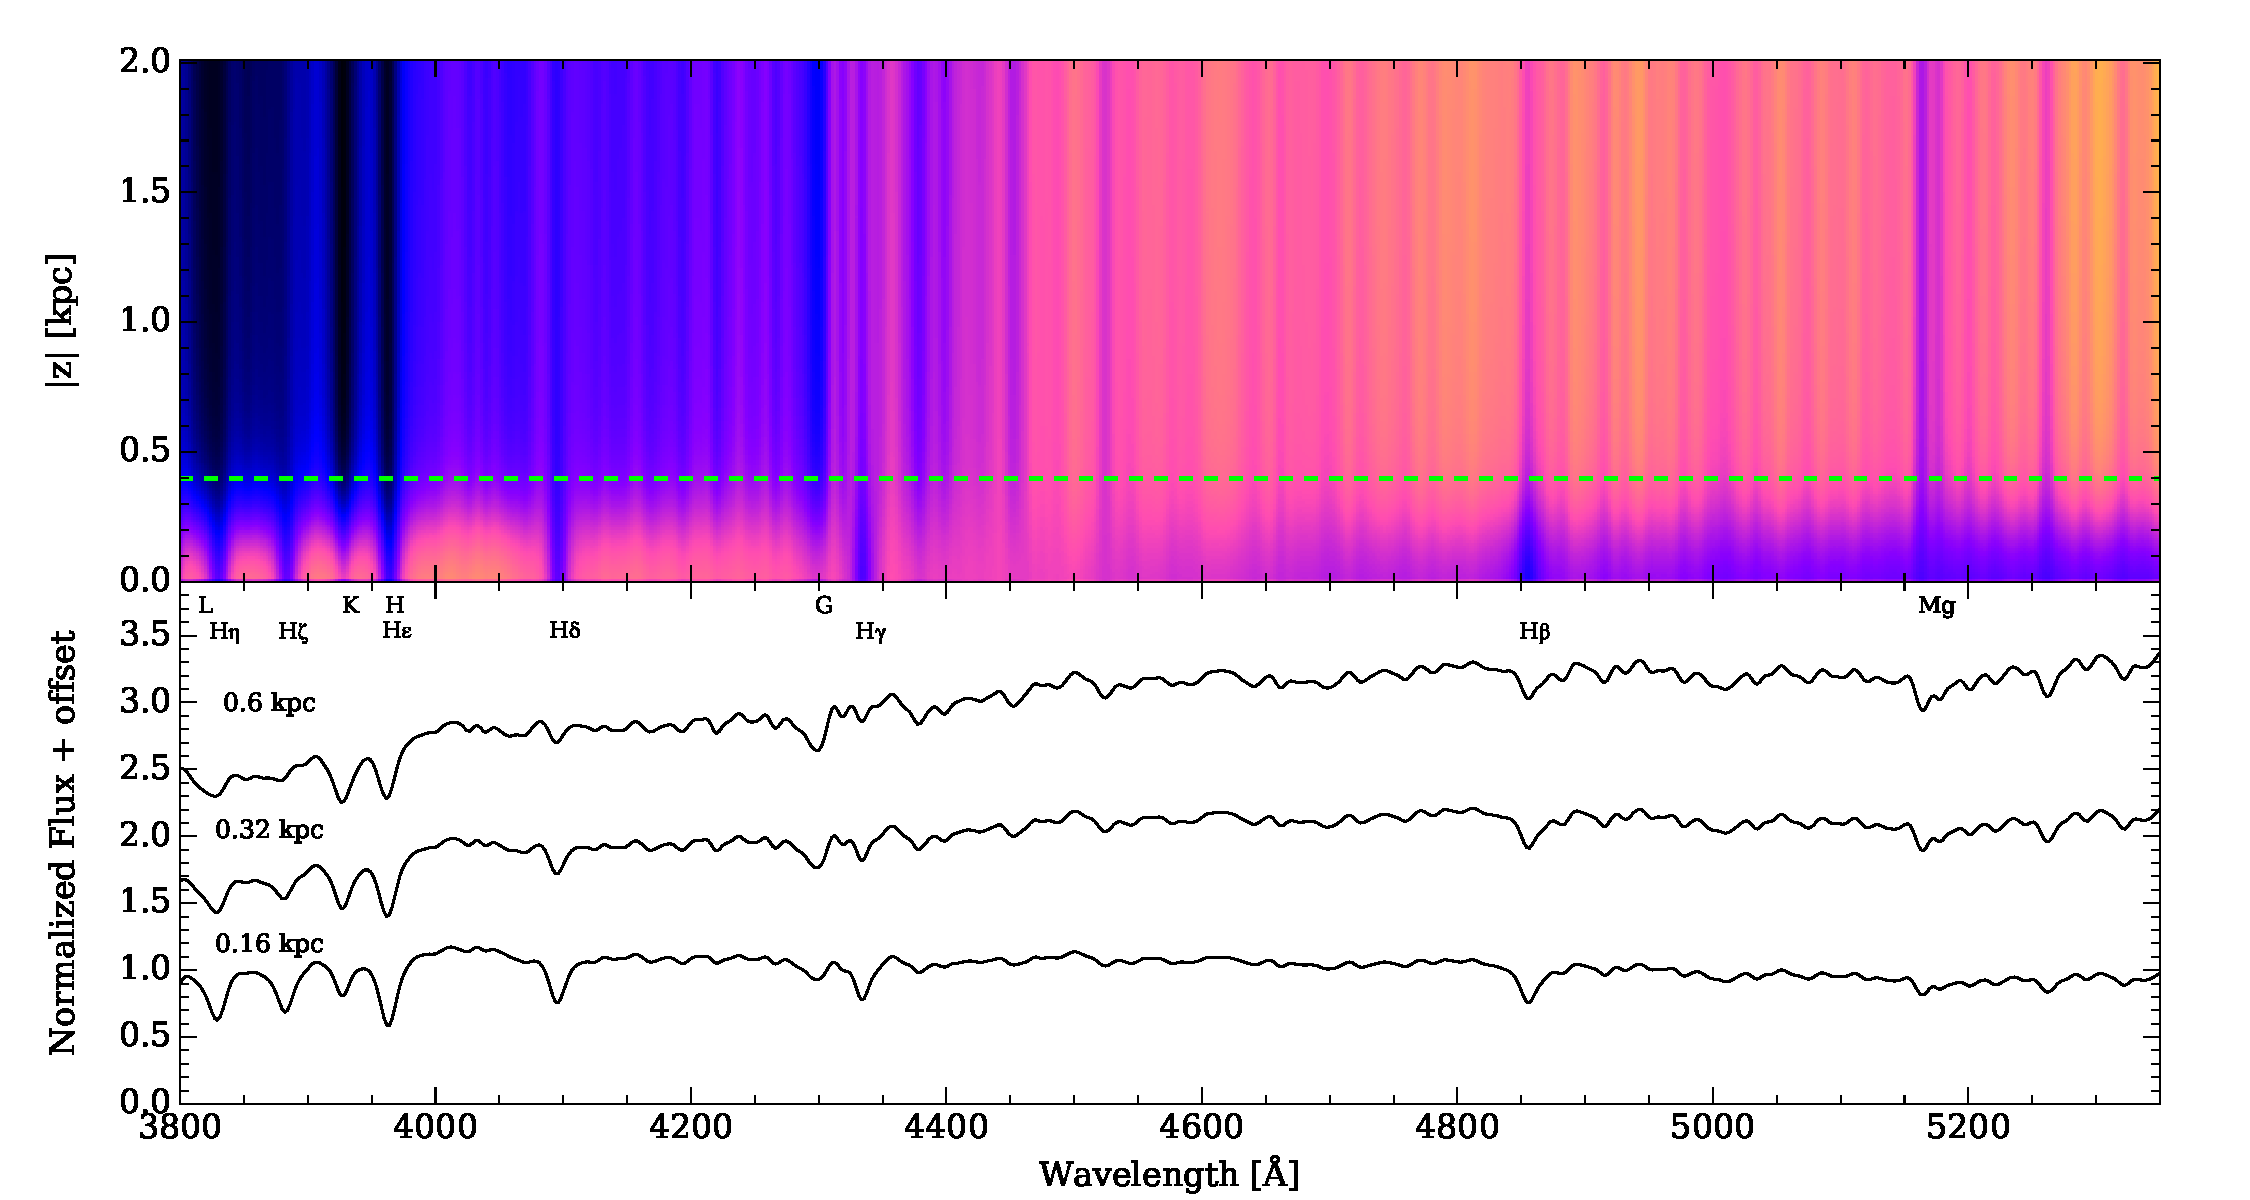
\includegraphics[width=\textwidth]{891_1/figs/mab_stack.pdf}
  \caption[Heating signature in Milky Way
  model]{\label{891_1:fig:MW_heating}\fixspacing Example of
    spectrophotometric index change with height and stellar
    population. Spectra are from a model with a fast-rotating (200 km
    s$^{-1}$) disk with a constant star-formation rate and a MW-like
    disk-heating rate, rendered at a spectral resolution of 200 km
    s$^{-1}$ ($\sigma$).  \emph{bottom:} Note the transition from
    Balmer-line to metal-line dominance between 0.32 and
    \val{0.6}{kpc}. \emph{top:} The same model spectra plotted with
    height and color-coded by normalized intensity. The transition
    between Balmer-line and metal-line dominated populations is clear
    in \Hda and Ca H\&K. Our models predict the location of the
    transition is a measure of the disk heating time-scale and is
    largely independent of the details of the star-formation
    history. The green line shows the same transition in NGC 891 at
    \val{0.4}{kpc} as discussed in \S\ref{891_1:sec:results}.}
\end{figure*}

%%
%%
%% Now in Thesis introduction
%%
%%
%% By the middle of the last century it was well established that the
%% scale-heights and velocity dispersions of stars in the solar
%% neighborhood increase with age \citep[see][for a summary of this early
%%   work, particularly the chapters contributed by Elvius and
%%   Delhaye]{Blaauw65}. The seminal work by \citet{Roman50} demonstrated
%% that the disk kinematics also depended on metallicity.  Today these
%% patterns are known in the literature on Galactic archaeology as
%% age-velocity-metallicity (abundance) relations \citep[AVM$\alpha$-R;
%%   e.g.,][]{Aumer09,Minchev14}. Observational advances continued for
%% the solar neighborhood \citep[e.g.,][]{Edvardsson93, Dehnen98,
%%   Nordstrom04}, and by the beginning of this century the complexity of
%% these relations have been mapped throughout much of Milky Way (MW) by
%% wide-field spectroscopic surveys (e.g., RAVE, \citealt{steinmetz06a};
%% BRAVA, \citealt{howard08a}, SEGUE, \citealt{yanny09a}, LAMOST,
%% \citealt{zhao12a} GALAH, \citealt{desilva15a},
%% Gaia-ESO,\citealt{gilmore12a}; and APOGEE-1 and -2,
%% \citealt{Majewski15}). The radial gradients in these relations are
%% beautifully shown by, e.g., by \citet{Bovy12c} and \citet{Hayden15},
%% illustrating both metallicity and abundance as well-known
%% complementary chemical-evolutionary tracers. Despite a century of
%% remarkable progress, two broad but intertwined questions remain: (i)
%% What are the astrophysical processes (i.e., the chemo-dynamical
%% explanation) leading to the observed relations; and (ii) are these
%% patterns generic for spiral disks or specific to the Milky Way?

%% Setting aside chemical evolution for simplicity, there has been a
%% long-standing debate about the origin of the vertical stratification
%% of disk stars in phase-space as a function of age (the age-velocity
%% relation, or AV-R). Historically the argument has been in the context
%% of dynamical heating from two-body scattering \citep{Spitzer51}, but
%% the scattering source has been debated \citep[e.g., giant molecular
%%   clouds, transient spiral structure, or dwarf satellite
%%   galaxies][]{Spitzer51,Spitzer53,Wielen77,Quinn93,Binney00}, and none
%% have proven satisfactory to explain the MW's thick disk.  This
%% framework has been salvaged but also up-ended by relatively recent
%% evidence for the increasing turbulence (and presumably thickness) of
%% ionized gas in disks at higher redshift
%% \citep{Weiner06,Forster-Schreiber09,Wisnioski15}. It seems plausible
%% that early phases of disk formation involved gas cooling, leaving
%% behind an old thick-disk stellar component
%% \citep{Brook04,Bournaud09}. However, thinner relic layers would also
%% emerge as time progressed \citep{Bird13}, depending critically on the
%% cooling time-scale for the gas in the presence of star-formation, AGN
%% feedback, and accretion, but without invoking any need for dynamical
%% heating. Ironically, this `settling' of the stellar disk with
%% population age is not unlike the predictions of monolithic collapse
%% from \citet{ELS}, albeit now consistent in the context of bottom-up,
%% or hierarchical structure formation as seen in recent simulations
%% \citep[e.g.,][]{Bird13,Martig14a}.  Because it is no longer clear if,
%% loosely speaking, disks `heat' or `cool' to form the the vertical
%% stratification of disk stars in phase-space, and likely both modes
%% play a role at late and early times, respectively, henceforth we refer
%% instead to `dynamical stratification' as a phenomenon that captures
%% both general physical processes.

%% The recent simulations noted above show there is a rich history of
%% radial and vertical build up of stellar populations that involves and
%% interplay between the cooling of the gas, the impact of mergers and
%% accretion, and at late times the classical heating processes noted
%% above.  This richness suggests the possibility for a diversity of
%% astrophysical paths in disk formation that could lead to significantly
%% different structure in galaxies, exhibited in their
%% AVM$\alpha$-Rs. Hence, the broader question of whether the MW is
%% representative of the external disk galaxy population becomes salient.

%% Little is known about the dynamical stratification rates for stars in
%% spiral outside the Milky Way, but recent studies of stellar
%% populations and dynamical stratification in low-mass spiral galaxies
%% \citep{Seth05a,Bernard15} have shown dramatic differences in the
%% age-metallicty and age-velocity dispersion relations when compared to
%% the Milky Way. Recent measurements of the stellar velocity dispersions
%% in M31 \citep{Dorman15} show that there are also gradients in
%% dispersion with age and metallicity, but the amplitudes and
%% time-scales are larger than in the MW. Differences in velocity
%% dispersion amplitudes may reflect a more massive or thinner M31 disk,
%% but possibly also a different dynamical history -- for gas settling or
%% stellar dynamical heating. Clearly more data on the stellar properties
%% of external galaxies is needed. The above studies serve as a gold
%% standard since they are based on studies of resolved stellar
%% populations. Because there are no massive spiral galaxies outside of
%% the Local Group for which we can resolve stellar populations at
%% surface-densities high enough to probe most of the disk, it is
%% imperative to undertake studies based on integrated starlight.

% Underpinning stellar dynamical mass estimates are assumptions about
% the distribution of matter in phase-space. Of importance are the
% density distribution and orbital anisotropy of the luminous tracers
% (Emsellem et al. 2011), both difficult to infer because of geometric
% projection. Typical mass-modeling assumptions include dynamical
% equilibrium, constant $\Upsilon_*$ and orbital anisotropy.  In
% star-forming disks there is every reason to believe these assumptions
% are invalid, even in the vertical direction where luminous young
% stars, gas and dust are in a thin mid-plane layer embedded in
% successively older, thicker, and dynamically warmer stellar
% populations \citep{Mihalas68,Wielen77,Binney00}. Disk components are
% expected to diffuse in a secular fashion through a dynamical heating
% process, forming layers in phase-space. Galaxy disks provide a unique
% laboratory for testing mass-modeling assumptions because they are
% dynamically cold, while on-going star-formation ensures that all
% phases of stellar evolution are present. What is critical is to
% measure the heating rate.

% For the younger and intermediate-age disk components which, for a disk
% like the MW, contains most of the light and a significant amount of
% the stellar disk mass over a modest range of metallicity (and
% therefore plausibly similar IMF). The heating time-scale over the past
% 4-6 Gyr in the solar neighborhood is comparable to the disk radial and
% vertical dynamical time-scales \citep{Aumer09}; even quiescent disks
% are not in true equilibrium. Determining disk heating rates pins down
% vertical gradients in $\Upsilon_*$ to within some {\it constant} scale
% factor (the IMF), thereby enabling a conversion from luminosity to
% {\it relative} density profiles.

% The main thrust of this program is to exploit vertical population
% gradients in star-forming disks to establish disk-heating rates. This
% will provide constraints on the cause(s) of heating, and eliminate
% systematics from our determination of disk gravitational potentials
% and thereby accurately calibrate $\Upsilon_*$. This can be done by
% combining spectroscopic indices that correlate stellar age to their
% kinematics and spatial location: By using integrated starlight as a
% {\it chronometer} it is possible to determine the dynamical evolution
% of disks. Because $\Upsilon_*$ evolves with stellar population age
% independent of uncertainties in the low-mass end of the IMF, such
% measurements decouple IMF uncertainties from the interplay between the
% relative distribution of luminosity and the dynamically-inferred
% mass. In other words, by measuring disk heating rates we will be able
% to distinguish between the mass-weighted scale-height of the disk and
% luminosity-weighted scale-height of our dynamical tracers.  To measure
% disk-heating and apply the results to an accurate mass-decomposition
% of spiral disks our program has this two-step framework:
% 
% \leftskip=0.35in
% {\it                                                                            
%                                                                                 
% \medskip                                                                        
% \noindent (i) determine the vertical age gradients and hence the disk
% heating rate in detail for a small but representative sample of
% $\sim$20 edge-on galaxies; and then
%                                                                                 
% \medskip                                                                        
% \noindent (ii) calibrate a proxy for stellar velocity dispersion
% applicable to large samples of star-forming galaxies at all
% inclinations, and to young stars and old stars. Use this proxy to
% constrain heating rates and dynamical models of stellar disks to infer
% their mass-density.
% 
% }
% \leftskip=0in

\subsection{Experimental Design}

In this paper we present a detailed, spectroscopic study of stellar
populations in the nearby, edge-on galaxy NGC 891 in integrated
starlight mapped over much of the visible stellar disk in both radius
and height. The importance of looking at NGC 891 as well as other
nearby edge-on disks is several fold. First, it allows us to expand
the census of spiral disks beyond the Local Group, particularly for a
geometric projection that allows us to examine the spatial gradients
in both radius and height more directly than in either M31 or the MW.
Second, NGC 891, while historically called out as a nearby MW analog,
clearly has some properties that are exceptional such as a large HI
scale height \citep[$\sim$1 kpc][]{Oosterloo07}, consistent with an
extended dust layer \citep{Howk00}. Measurements of vertical and
radial population gradients in NGC 891 will provide a better picture
of the range of such gradients in MW-like systems, pointing to the
range and multiplicity of disk formation and assembly scenarios of
MW-like galaxies.

As a benchmark for what we might expect to see in terms of
AVM$\alpha$-R in the integrated light of an external, edge-on galaxy,
for illustration purposes we focus again simply on age and velocity
(AV-R, where velocity, i.e., velocity dispersion is rendered in
equivalent height given relevant dynamical assumptions) and ask: If
NGC 891 has a similar star-formation history and AV-R as the MW's
solar cylinder, what would the integrated light look like if observed
edge-on? In answering this question here, our intent is demonstrate
the essence of our experimental design, namely a method to measure
disk dynamical stratification rates by using stars as chronometers.

To estimate the vertical distribution of the stellar spectral energy
distribution we construct a simple model where stars in disks (i) form
at some rate at the mid-plane with a scale-height and velocity
dispersion comparable to the gas; and then (ii) are dynamically
stratified through some secular process over time. We adopt a constant
star-formation rate (SFR) and total age of 11 Gyr\footnote{This is a
  reasonable match for the total age of the MW disk and the
  star-formation formation rate over the past few Gyr based on
  analysis of stars in the solar cylinder
  \citep[e.g.,][]{Pilyugin96a}.}, the `heating' model for the solar
cylinder of \citet{Aumer09}, and we assume the dynamics are such that
$\sigma_z^2/h_z$ is constant at late times, which is roughly what is
observed in the MW disk near the sun ($\sigma_z$ is the vertical
stellar velocity dispersion and $h_z$ is the corresponding
scale-height, i.e., $\sigma_z^2/h_z$ is proportional to the surface
mass-density of the disk). We also adopt the stellar population
synthesis models of \citet{Bruzual03} but note in the spectral range
of interest here the choice is unimportant. By coupling elements (i)
and (ii) to stellar population synthesis models it is them possible to
compute the vertical distribution of star light.

In adopting this simplified model to represent what we might see for
the projected vertical distribution of integrated starlight of an
edge-on galaxy like NGC 891 we are in effect assuming the SFR and
dynamical stratification are constant with radius, which, despite the
apparent radial constancy of disk thickness observed over many radial
scale-lengths in external galaxies, at some level must be
incorrect. Certainly we know there is flaring in gas layers with
radius as well as gradients in the total and specific SFR.  In a
companion paper we discuss details about assumptions of the gas-layer
thickness between NGC 891 and the MW, radial variations in the
gas-layer thickness and heating rate, relative sensitivity to the
star-formation rate versus the heating rate, as well the general
problem of heating models' inability to match the thick disk, as noted
above. The simplifications adopted here allow us to look at what
appear to be the primary observational consequences of dynamical
stratification on vertical trends in the spectral energy distributions
of galaxies; this simple model is likely to capture the interplay of
stellar evolutionary time-scales and dynamical stratification that
dominate the younger and intermediate-age disk components in the MW
\citep{Bird13}.

We illustrate the spectrophotometric rendering of our simple model in
Figure \ref{891_1:fig:MW_heating}.  This example shows how the spectra of
integrated star-light would appear as a function of height above the
disk mid-plane for a dynamical stratification rate self-similar to what
is seen in the MW solar cylinder. Inspection shows there is a height
above the disk mid-plane where a rapid transition in the stellar
population occurs at roughly $|z| \sim 0.4$ kpc.  Here, the spectrum
evolves from Balmer-absorption to metal-absorption dominance on the
time-scale of A/F main-sequence stellar lifetimes ($\sim$0.5 Gyr). The
break-height where this occurs is relatively insensitive to
star-formation history, spectroscopic line-strengths are reddening
independent, and line-of-sight attenuation from dust at this expected
break-height is not prohibitive for detection.  Consequently,
measuring the break height yields a constraint on the dynamical
stratification rate on these time-scales. The transition is best
detected in spectra covering the 4000 \AA\ region, and can be
measuring easily even with low-resolution spectrophotometry.

Our first-order objective is to determine if we can detect and measure
a spectral break height in the disk of NGC 891, and if so, how it
compares to the this simple model for the MW solar cylinder. The
height and width over which the spectral break occurs yields a
constraint of AV-R, or the dynamical stratification rate at late
times. While this model may be qualitatively correct for the solar
neighborhood and NGC 891, it is well worth verifying if the observed
gradients are constant with projected radius.  It has been suggested
from the simulations of \citet{Martig14a} that the young, star-forming
disk at every epoch flares), likely for dynamical reasons perhaps
related to the flaring of atomic and molecular gas at the current
epoch. Recent measurements suggest such flaring is seen in MW stars
\citep{Ness16}. We will probe for a similar flaring in NGC 891,
manifest as a change in break height with radius.  While differential
extinction effects cannot be ignored when interpreting line-of-sight
depths of our observations, we will use Doppler tomography in Paper II
\citep[see for example,][]{Kregel05} to increase the fidelity of
our measurements in Paper II.

Our higher-order objective is to probe if the spectrophotometric data
of integrated starlight farther above the mid-plane enables us extend
constraints on the dynamical stratification over longer time frames
commensurate with the old thin and thick disks.  While the
implementation is beyond the scope of the present work, the detection
of metallicity and abundance gradients in both radius and height
provides a mapping of AVM$\alpha$-R in external galaxies, and, via the
appropriate chemo-dynamical model, constraints on the dynamical
stratification for disk stars over most of the star-formation history
of the galaxy.

In this paper we describe the custom fiber integral field unit we
built to make these measurements of vertical population gradients in
nearby, edge-on disks (Section \ref{891_1:sec:pak}).  Our observations of
NGC 891 with this IFU are described in section \ref{891_1:sec:obs}.  The
data reduction and calibration procedures, particularly those specific
to this first variable-pitch IFU, are given in section
\ref{891_1:sec:data_reduction}. The resulting spectral maps are binned based
on signal-to-noise (S/N) criteria motivated by astrophysically
motivated requirements on determining age and metallicity in the
integrated light of stellar populations, and determined via modeling
in Section \ref{891_1:sec:maps}. Spectral diagnostics are measured for these
binned spectra to examine of the trends in age, metallicity and
abundance with radius and height in Section \ref{891_1:sec:results}.  These
give a qualitative picture of the population gradients in this galaxy,
as projected along the line of sight. A synopsis of the results from
this paper are given in Section \ref{891_1:sec:summary}.  In an accompanying
paper we undertake spectral analysis to quantify the line of sight
depth of these observations, and the stellar population gradients in
this galaxy, comparing them to what we might expect in the Milky Way.

% For the younger and intermediate-age disk components which, for a disk
% like the MW, contains most of the light and a significant amount of
% the stellar disk mass over a modest range of metallicity (and
% therefore plausibly similar IMF). The heating time-scale over the past
% 4-6 Gyr in the solar neighborhood is comparable to the disk radial and
% vertical dynamical time-scales \citep{Aumer09}; even quiescent disks
% are not in true equilibrium. Determining disk heating rates pins down

% We use a simple heating model of \citet{Aumer09}, suitable for the MW
% solar cylinder, and based on Hipparcos proper-motion data and
% Geneva-Copenhagen radial velocities. For each cohort of disk stars,
% i.e., those that form at some epoch this yields a vertical velocity
% dispersion that grows as \citep[using the formulation
%   of][]{Wielen77} $$\sigma_z(t) = \sigma_z(0) (1+t/\tau_{\rm
%   heat})^{1/n_h},$$ where $\tau_{\rm heat} \sim 5 \times 10^7$ yr is
% the heating time-scale, $\sigma_z(0)$ is the velocity dispersion of
% the stars at birth, the exponent $n_h$ is referred to as the heating
% index, and time is moving forward from, and indexed to, the cohort
% formation epoch.

% Historically and physically, the model derives from
% \citet{Spitzer51,Spitzer53} molecular-cloud scattering scenario where
% the time-constant for energy transfer for the Solar neighborhood can
% be interpreted in terms of molecular cloud mass and density, the
% initial velocity-dispersion, and a complex function of $B/\omega$
% where $B$ is Oort's constant and $\omega = V_c/R$, i.e., the angular
% velocity. What is relevant here is that the formulation provides a
% simple, analytic model which describes well the phase-space
% stratification of MW disk stars.

% One further required model component relates the vertical thickness to
% velocity dispersion. We assume the dynamics are such
% that $\sigma_z^2/h_z$ is constant at late times, which is roughly what
% is observed in the MW disk near the sun, but that the stellar layer
% never gets thinner or dynamically colder than the gas layer at $h_z =
% 0.065$ kpc and $\sigma_z = 8$ km s$^{-1}$.  While the atomic gas layer
% in NGC 891 is vertically very extended \citep{Swaters97, Oosterloo07},
% the relevant thickness is the molecular gas, which in NGC 891 is much
% thinner, but about a factor of two thicker than the molecular disk in
% the MW \citep{Scoville93, Yim11}. This is a pretty good match to the
% near-infrared ($K$ band) super-thin disk component scale-height of 160
% pc found by \citet{Schechtman-Rook13}. Despite this difference, we
% scale the stellar vertical distribution as a function of their age
% such that they match the MW old thin-disk stars with $h_z = 0.350$
% kpc, $\sigma_z =20$ km s$^{-1}$, and an age of 7 Gyr.

% The specified heating model, however, is parameterized for the solar
% cylinder. In order for the disk to have constant thickness with
% radius, yet a velocity dispersion profile that is roughly exponential
% with twice the photometric scale length - what we observe for disks
% today - at least one of three parameters change with radius: the
% heating time-scale, the heating index, or the initial gas velocity
% dispersion. While any one of these can be modulated with radius to
% achieve a nearly constant vertical scale-height with time and radius,
% it is compelling to keep the heating- index constant (i.e., the
% physical heating mechanism is the same) while setting the heating
% time-scale to be the dynamical time-scale associated with the disk's
% rotation. Note for example that $\tau_{{\rm heat},\odot} \sim (\pi/2)
% R_\odot/V_\odot$ adopting $V_\odot = 220$ km s$^{-1}$ and $R_\odot =
% 8$ kpc as the circular speed and distance to the Galactic center at
% the Solar radius. Except for the inner portion of the galaxy,
% $\tau_{\rm heat}$ is simply a linear function of radius.

% It is also reasonable to adopt an initial velocity dispersion of the
% stars that has a modest trend with radius. This is plausible because
% the gas also exhibits such a trend, as seen by \citet{Shostak84}, and
% more recently updated by \citet{Tamburro09}. We will show elsewhere
% that this produces a time-evolution of a stellar disk that uniformly
% thickens while quickly developing a radial trend in stellar velocity
% dispersion that matches observations in the DMS.

% There is no chemical evolution in the model, but it would be
% straight-forward to add following, e.g.,
% \citet{Pilyugin96a,Pilyugin96b,Chiappini97} based on the earlier
% studies of \citet{Twarog80, Carlberg85,
%   Meusinger91,Edvardsson93}. From these studies, it is reasonable to
% approximate the age-metallicity relation as linear in time with [Fe/H]
% = 0.05 today and [Fe/H] -0.35 8 Gyr ago, then dropping rapidly at
% earlier ages where it would be reasonable to adopt Z = 0.2 solar.

% $h_z(t=7{\rm Gyr})=0.35$ kpc $\sigma_z(t=7{\rm Gyr}) = 20$ km
% s$^{-1}$ Then $\sigma_z(t=0)$ is inferred from $\sigma_z(t=7{\rm
% Gyr})$ using the heating model, but not allowed to be less than
% $sigma_{z,{\rm min}} = \sigma_{\rm gas} / \sqrt{1/a^2+2/3)$ km
% s$^{-1}$, where $a = 0.6$ (why?). The thicknes is given by $h_z(t) =
% h_z(t=7{\rm Gyr})(\sigma_z(t)/\sigma_z(t=7{\rm Gyr}))^2$, with the
% additional imposition that $h_z(t) \geq h_{z,{\rm min}} = 0.065$
% kpc, i.e., the gas layer in the MW, which at least for HI in N891,
% is not a good match. However the relevant thickness is the molecular
% gas, which in NGC 891 is comparable to the MW (Scoville et
% al. 1993).
% 
% For $n_h = 3$, $\tau = 0.05$ Gyr, while for $n_h = 2$, $\tau = 0.2$
% Gyr. These values are from Wielen (1977), but the $n_h = 3$ case is
% consistent with Binney et al. (2000) analysis of Hipparcos data.
% Further, this value of $\tau$ is close to the dynamical time-scale
% $t_{\rm dyn} = 2 \pi R/V$ at the solar circle ($R = 8$ kpc, $V = 220$
% km s$^{-1}$).

% another paper to look at for asymmetry and high-z dust: Hughes et al. 2014

%% \begin{figure}
%%   \centering
%%   \includegraphics[width=\columnwidth]{figs/mab_plot_model.pdf}
%%   \includegraphics[width=\columnwidth]{figs/mab_plot_modelspec.pdf}
%%   \caption{\label{fig:MW_heating}Example of spectrophotometric index change
%%     with height and stellar population. Spectra are from a model with a
%%     fast-rotating (200 km/s) disk with a constant star-formation rate and a
%%     MW-like disk-heating rate. Note the transition from Balmer-line to
%%     metal-line dominance between 0.8 and 1.5 hz. Our models predict the
%%     location of the transition is a measure of the disk heating time-scale and
%%     is largely independent of the details of the star-formation history.}
%% \end{figure}

%% \begin{figure}
%%   \centering
%%   \includegraphics[width=\columnwidth]{figs/mab_plot_model.pdf}
%%   \caption{\label{fig:mab_model}Another view of the spectrophotometric
%%     index change shown in Figure \ref{fig:MW_heating}. Color is mapped
%%     to intensity and all spectra have been normalized to unity mean
%%     over the wavelength interval shown. The horizontal line marks the
%%     age break at \val{0.4}{kpc} found in
%%     \S\ref{891_1:sec:results}. This break is remarkably consistent with the
%%     transition from Balmer-line to metal-line (Ca H\&K) dominance seen
%%     the models.}
%% \end{figure}

 





\section{The \GP Variable-Pitch IFU}
\label{sec:pak}

\subsection{Design}
\label{sec:GP_design}

\begin{figure*}[t]
  \centering
\vskip -0.65in
  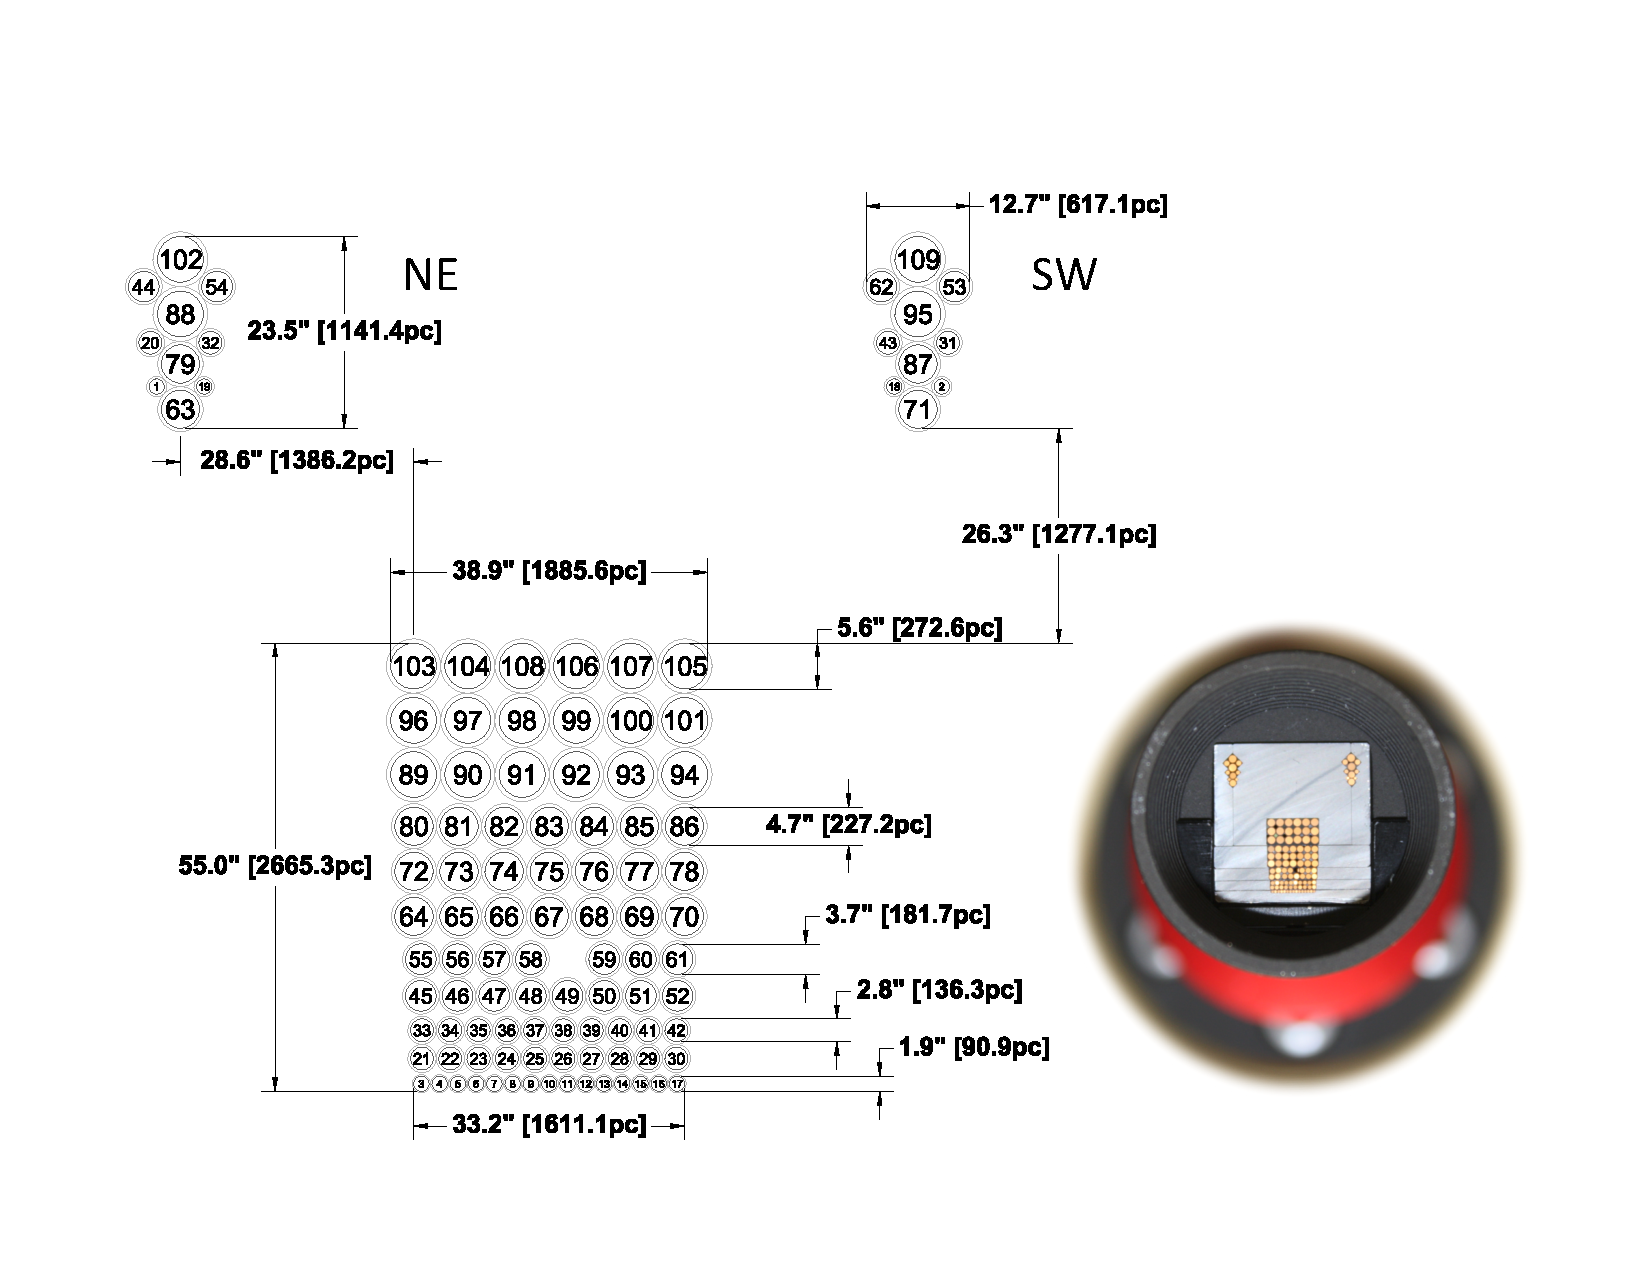
\includegraphics[width=\textwidth]{891_1/figs/GradPak_labeled_inset_ALT.pdf}
\vskip -0.35in
\caption{\label{fig:GradPak}\fixspacing\GP IFU on the WIYN 3.5m
  Telescope. Distances are in arcseconds and in kpc for a distance of
  10 Mpc. The inset image shows the completed IFU in its mounting
  bracket. Note aluminum fixture and absence of packing fibers.}
\end{figure*}

The \GP integral field unit (IFU) is mounted on the WIYN\footnote{The
  WIYN Observatory is a join facility of the University of
  Wisconsin-Madison, Indiana University, NASA, and the National
  Optical Astronomy Observatory.}  Bench Spectrograph
\citep{Barden94,Bershady08,Knezek10} and makes up one half of the
novel HexPak/\GP IFU system \citep{Wood12}, a pair of IFUs that have
unique fiber configurations and share a common slit. The fiber
geometry of \GP is optimized for observations of edge-on galaxies;
five different fiber sizes are arranged in a rectangular gradient
pattern that allows for efficient observations of objects with
significant surface brightness gradients on scales of roughly an
arcminute (Figure \ref{fig:GradPak}).  A list of fiber diameters can
be found in Table \ref{tab:GradPak}. The increase in fiber size across
the array corresponds to equal signal-to-noise (S/N) per unit
wavelength in the source or background-limit for light distributions
with e-folding scales of 26 to 50 arcsec. This corresponds to vertical
scale-heights of 1.3 to 2.4 kpc at a distance of 10 Mpc, comparable to
the thickest possible disk components in NGC 891.  In practice, the
complex vertical structure of stars and dust in galaxy disks such NGC
891's make the S/N optimization imperfect. This instrument design, by
attempting to achieve similar signal-to-noise per exposure in all
fibers, maximizes mapping efficiency at the cost of reduced spatial
and spectral resolution in the larger fibers at larger
scale-heights. This trade-off is sensible given the increased
e-folding scale of the disk away from the mid-plane, and the
commensurate expectation of large velocity dispersions.

The physical layout of \GP consists of a main array and two groups of
offset sky fibers. The main array is a 55 arcsec high stack of pseudo
slits with increasing slit-width and fiber diameters (Figure
\ref{fig:GradPak}). The fibers used are broad spectrum, stepped index,
fused silica fibers (Polymicro FBP) with core diameters between
\val{200}{\mu m} and \val{600}{\mu m} (corresponding to \val{1.87}{''}
to \val{5.62}{''} at the WIYN f/6.3 focal plane). The non-active
(i.e., cladding and buffer) portion of each fiber takes up an
additional 20\% of each fiber's physical diameter. The pseudo-slits
are grouped into blocks that contain all the fibers of the same
size. The blocks were assembled sequentially from small to large fiber
sizes to build up the entire stack. Each block is mechanically bounded
by precision layers of aluminum, located with pins. The smallest
fibers have only one row (or pseudo-slit) that is 33.2 arcsec in
length; the two largest fibers sizes have three rows each, with a
maximum pseudo-slit length of 38.9 arcsec; while the intermediate
sizes have two rows. After a block has been assembled, glued and
cured, it is separated from the next block by a plastic shim that is
\val{25.4}{\mu m} (\val{0.24}{''}) thick; this separation is a key
component of the assembly and curing process.  While the scientific
design of \GP required a non-optimal fiber packing arrangement, the
total packing efficiency (defined as light-gathering area divided by
total area) of the main array is roughly 55\%.

The sky fibers of \GP occupy two sub arrays that are offset
\val{26.3}{''} vertically and \val{28.6}{''} horizontally on either
side of the main array. On NGC 891 this places the sky fibers
\val{1.3}{kpc} above the top of \GP and \val{\sim 3.8}{kpc} from the
plane of the galaxy, far above measurable flux from the galaxy
\citep{Rand11}. The sky fibers were assembled separately in machined
blocks that are mechanically attached to the main array. This assembly
was polished as a single, assembled unit. The polishing process was
similar to what was undertaken for SparsePak \citep{Bershady04}.

\GP does not have any packing fibers. Instead, the physical layout is
established with a custom-built aluminum fixture, as described above
and in \citep{Wood12}. Based on the results of
\S\ref{sec:gradpak_performance} we do not think the lack of buffering
fibers causes a significant loss of performance. However, the use of
aluminum, and in particular the aluminum shim material comprising the
walls of the pseudo-slit layers is not optimal for optical polishing,
with deleterious effects noted in \S\ref{sec:gradpak_performance}. A
lesson learned is that the fabrication ease, efficiency and low
machining cost of aluminum does not out-weigh the superior performance
of suitable stainless steel, invar or ceramics, which we would
recommend for future builds. In contrast, for example, the stainless
steel ferrules used in MaNGA in SDSS-IV provided outstanding fixturing
for obtaining good optical finish on the polished fibers (Drory et
al. 2014).  We note that the challenges with the aluminum fixture for
\GP is was not an issues for HexPak which, like its predecessors
DensePak (Barden et al. TODO) and SparsePak (Bershady et al. 2004)
consisted of an entirely fused-silica array.

Further details of the design and construction of HexPak/\GP,
including cable design, fabrication and commercial product
descriptions for specific components can be found in \citet{Wood12}.
Notable are the dual-slit assembly that sits inside a standard Bench
Spectrograph fiber ``foot,'' as well as the rotation couplers that
ease handling will minimizing stress-inducing torsion on the fibers
during telescope rotator motion.

\begin{deluxetable}{ccccc}
\tablewidth{0pt}
\tablecaption{\GP Fiber Diameters}
\tablehead{
  & 
  \colhead{spatial} &
  \colhead{spectral\,\tablenotemark{a}} &
  &  \\
  \colhead{($\mu$m)} &
  \colhead{(pixels)} &
  \colhead{(pixels)} &
  \colhead{(arcsec)} &
  \colhead{(pc\,\tablenotemark{b})}
}
\startdata
200 & 4.64 & 4.36 & 1.87 & 90.9\\
300 & 6.96 & 6.55 & 2.81 & 136\\
400 & 9.28 & 8.73 & 3.75 & 182\\
500 & 11.6 & 10.9 & 4.69 & 227\\
600 & 13.9 & 13.1 & 5.62 & 273
\enddata
\label{tab:GradPak}
\tablenotetext{a}{\fixspacing Assuming the anamorphic factor in Table \ref{tab:spec}}
\tablenotetext{b}{\fixspacing Assuming a distance of \val{10}{Mpc} to NGC 891.}
\end{deluxetable}

\subsection{Mechanical Performance}

Despite best effort and extensive testing to develop best practices,
the mechanical alignment of the \GP fibers has some noticeable
imperfections. In Appendix \ref{sec:GPtesting} we provide a
high-resolution image (Figure \ref{fig:gradpak_face}) of the as-built
fiber array to document this. The irregularities are particularly
notable for the 400 $\mu$m (3.75 arcsec) fiber pseudo-slits for which
some fibers have offsets from their idealized location (Figure
\ref{fig:GradPak}) by as much as 0.5 arcsec. The other pseudo-slits
have internal and relative alignment to other pseudo-slits that we
estimate are accurate at the 0.l-0.2 arcsec level. Table
\ref{tab:GP_cal} in the Appendix provides the
idealized fiber locations corresponding to Figure
\ref{fig:GradPak}. These should suffice for almost all applications
except the most demanding that for whatever reason require very high
precision relative astrometry. Should the need arise, Figure
\ref{fig:gradpak_face} will be made available upon request. Overall,
the final IFU has good-to-excellent mechanical regularity.

\subsection{Optical Performance}

\label{sec:gradpak_performance}

The IFU face and slit were both polished to a \val{0.5}{\mu m} grit
level to mitigate throughput losses caused by surface scattering
\citep{Eigenbrot12}. Material from the aluminum fixture was seen to
form deposits on the fiber faces, with some performance degradation
that we summarize here and detail in Appendix \ref{sec:GPtesting}.

Laboratory measurements of throughput and focal-ratio degradation
(FRD) in the Johnson $V$ revealed distinct performance gradients
across the array. Some of the throughput variations are likely due to
polish imperfections from aluminum residue. However, we find FRD
systematically decreases with larger fiber size, with a small upturn
for the largest fibers. Unfortunately we cannot separate systematic
performance differences for different fiber core sizes from
differences in handling and assembly process. We also find, not
surprisingly, that FRD correlates to first order with throughput, but
that there is a bimodal distribution in transmission and FRD which
indicates several processes at work in determining fiber performance.

Overall, the throughput defined for $f$/6.3 fiber input from the
telescope and the $f$/4 out speed matching the Bench Spectrograph
collimator has a maximum of 90\% and a minimum of 50\% at 550 nm. The
mean throughput for all fibers is 80\%, with means by fiber size of
70, 81,84, 83, 79\%, from small to large. Means for sky fibers are
comparable, within a percent. We compared our lab measurements to the
relative throughput from dome-flats measurements once \GP was
installed on the telescope. This comparison shows that the
on-telescope {\it relative} performance is the same, indicating
throughput variations are intrinsic to the cable and not the
spectrograph, consistent with expectations for the performance of the
upgraded Bench Spectrograph \citep{Bershady08,Knezek10}.

One of the 3.75'' fibers (between fibers 58 and 59 as marked in Figure
\ref{fig:GradPak}) fractured during polishing. The fracture is close
to the surface and likely could be polished out; this was deemed
impractical to pursue due to the indeterminate fracture depth and the
risk of exceeding the finite gluing length. The fracture leaves 10\%
of the fiber face intact and transmitting, but for practical purposes
this fiber is considered not usable and ignored in all astrometry
tables.  A close-up image of the \GP fibers that shows polishing
imperfections and the broken fiber can be found in Figure
\ref{fig:gradpak_face}.  Despite these imperfections, the final IFU
has good transmission performance.

\subsection{Installation}
\label{sec:install}

Final construction of \GP was completed in September 2013.  HexPak/\GP
were then installed at WIYN during November 2013. The 25 m of cabling
that contain the IFUs are routed from the Bench Spectrograph room, up
through the central bearing of the azimuth drive, out of one of the
telescope forks, and onto a tray designed to hold the SparsePak
cable. During observations one of the IFU heads is plugged into the
the WIFOE\footnote{WIYN Indiana Fiber Optic Echelle} port, which
provides common IFU access to the IAS\footnote{Imaging Acquisition
  System} on one of WIYN's nasymth ports. During cable routing a
section of cabling developed a hole that was the result of bend stress
causing the helical wrapping of the cable to come undone. This hole
was repaired on site and is located just within the fork on the
observing floor. Fibers were not damaged, and the cable integrity has
been deemed acceptable for the life of \GP.

During installation we confirmed that both the HexPak and \GP slits
occupy the same focal plane, which allows the heads to be switched at
the telescope end without the need to adjust the Bench Spectrograph.
We also adjusted the precise location of the HexPak, \GP, and
SparsePak \citep{Bershady05} fiber faces so that they share a common
focus in the port. The common focus locations at both ends of the
fiber cable allow users to switch between HexPak and \GP in only a few
minutes during the night, which allows great flexibility in scheduling
multiple programs on the same night.

In addition to access for the WIYN IFUs the WIFOE port has a pellicle
and camera that allow observers to see an image of the IFU fibers
overlaid on the view from the telescope focus. To resolve the smallest
fibers in HexPak/\GP the existing WIFOE camera was replaced with an
Allied GigE GT3300 CCD with a default resolution of
0.258''/pixel\footnote{more information can be found at
  \url{http://www.wiyn.org/Instruments/WifoeCameraInterface.pdf}}.


\section{Observations} 
\label{891_1:sec:obs}

Observations of NGC 891 were obtained over two runs in November and
December of 2014. Data were collected with the \GP IFU, coupled to the
WIYN Bench Spectrograph.

\begin{deluxetable}{lcc}
\tablewidth{0pt}
\tablecaption{Spectrograph Setup}
\tablehead{
  \colhead{Parameter} &
  \colhead{Value} &
  \colhead{Units}
}
\startdata
Grating Name & 400@4.2 & -\\
Order & 1 & -\\
Grating Angle & 21.53 & deg.\\
Camera-Collimator Angle & 30.00 & deg.\\
Anamorphic factor & 0.941 & -\\
$\lambda_\mathrm{min}\tablenotemark{a}$ & 3372 & \AA\\
$\lambda_\mathrm{max}\tablenotemark{a}$ & 7640 & \AA\\
Dispersion at \val{5500}{\AA}\tablenotemark{b} & 2.079 & \AA/pix
\enddata
\label{891_1:tab:spec}
\tablenotetext{a}{Formal wavelength range; values
  used for analysis are between 3850 and 6650\AA\ as described in the
  text.} 
\tablenotetext{b}{For 2$\times$ binning in the spectral dimension.}
\end{deluxetable}

\begin{deluxetable}{ccllc}
\tablewidth{0pt}
\tablecaption{Program Targets}
\tablehead{
  \colhead{Name} &
  \colhead{Type} &
  \colhead{$\alpha$} &
  \colhead{$\delta$} &
  \colhead{epoch}
}
\startdata
NGC 891 P1 & object & 02:22:29.7 & +42:19:17.2 & 2000\\
NGC 891 P2 & object & 02:22:32.5 & +42:20:26.0 & 2000\\
NGC 891 P3 & object & 02:22:37.6 & +42:22:38.3 & 2000\\
NGC 891 P4 & object & 02:22:30.1 & +42:21:33.7 & 2000\\
NGC 891 P5 & object & 02:22:26.8 & +42:18:07.9 & 2000\\
NGC 891 P6 & object & 02:22:40.4 & +42:23:57.0 & 2000\\
BD 284211 & flux standard & 21:48:57.1 & +28:37:48.0 & 1950\\
Feige 110 & flux standard & 23:17:23.5 & -05:26:22.0 & 1950
\enddata
\label{891_1:tab:targets}
\end{deluxetable}

\subsection{Spectrograph Configuration}

For both runs the spectrograph was configured identically to cover as
far blueward of the 4000\AA-break as practically possible while
reaching as far red as H$\alpha$.  The scientific motivation for this
large baseline was to capture Ca H\&K (3934,3968 \AA; this also
includes H$\epsilon$), the G-band ($\sim$4304 \AA), MgI
($\sim$5175 \AA), and the upper Balmer series (at least up to
H$\delta$), all important diagnostics for stellar populations; to
provide a measure of the continuum slope to determine reddening
independent of stellar age; and to have additional checks on the
extinction as derived from the ratio of \Ha/\HB emission line fluxes
(i.e., the Balmer decrement).

Achieving such a broad wavelength range that extends to the blue with
the Bench Spectrograph is challenging. This is due primarily to the
decreasing transmission of the spectrograph optics and fibers and
decreasing CCD quantum efficiency below 4500 \AA. In addition, as a
single beam spectrograph with all-refractive optics, the ability to
focus over a broad wavelength range extending to the blue is limited,
despite the ability to tilt the detector to compensate for chromatics.
Lastly, the grating suite is not optimal. Two 600 l/mm gratings are
just able to capture from, e.g., 3800-6650 \AA, which would enable us
to just capture the Fraunhofer L-band and H$\eta$ features between
3810-3840 \AA\ in the blue, and the redder [NII] line at 6584 \AA\ in the
red. Unfortunately these gratings are blazed too far to the red to
provide adequate overall efficiency in the blue.

We used engineering time to test alternative spectrograph
configurations with improved performance in the blue.  As we show in
Appendix \ref{891_1:sec:grating} compared to the best alternative 600 l/mm
grating, the very low (blue) blaze of the 400@4.2 grating yields
better performance below 4500 \AA\ (a factor of 2 increase in total
system efficiency at 4000 \AA), and broader wavelength coverage, albeit
with a 37\% lower spectral resolution. Because of the importance of
the blue spectral region, we chose this grating for our
observations. The detailed configuration provided in Table
\ref{891_1:tab:spec}.

While our spectrograph configuration covers between 3372 and 7640 \AA\
(the blaze wavelength is 3496 \AA) on the detector, in practice the
useful blue limit of the data is roughly \val{3850}{\AA} due to the
sharp decline in system efficiency. This captures H$\zeta$ and
sufficient pseudo-continuum to define a break amplitude \citep[e.g.,
$D_n4000$;][]{Balogh99}. The Fraunhofer L-band and H$\eta$ features
between 3810-3840 \AA\ are clearly visible in the highest
signal-to-noise data, while the strong FeI blends in the 3700-3750
\AA\ region and the Balmer break (3646 \AA) are not detected.  At the
red end of our wavelength range defocus becomes a serious problem and
fiber traces begin to blend significantly. This defocus, and the rise
of strong atmospheric OH features, sets the usable red limit to
\val{6650}{\AA}; this still captures \Ha and [NII] lines.

\subsection{Targeting}
\label{891_1:sec:targeting}

\begin{deluxetable}{cccll}
\tablewidth{0pt}
\tablecaption{Summary of Observations}
\tablehead{ 
  \colhead{Pointing} & 
  \colhead{Date} & 
  \colhead{$r$} & 
  \multicolumn{2}{c}{Integration (min)}\\
  \colhead{} &
  \colhead{(UT)} &
  \colhead{(kpc)} &
  \colhead{Nightly} &
  \colhead{Total}
}
\startdata 
1 & 2014 Nov 20 & 4.4      & 210 & $\cdots$ \\
  & 2014 Nov 21 & $\cdots$ &  60 & 270 \\
2 & 2014 Nov 21 & 0.8      & 210 & $\cdots$ \\
  & 2014 Nov 22 & $\cdots$ &  60 & 270 \\
3 & 2014 Nov 23 & $-6.4$   & 330 & 330 \\
4 & 2014 Nov 24 & $-2.3$   & 270 & 270 \\
5 & 2014 Dec 20 & 8.1      & 270 & $\cdots$ \\
  & 2014 Dec 22 & $\cdots$ & 270 & 540 \\
6 & 2014 Dec 21 & $-10.0$  & 240 &  $\cdots$ \\
  & 2014 Dec 23 & $\cdots$ & 120 & $\cdots$ \\
  & 2014 Dec 24 & $\cdots$ & 180 & 540
\enddata
\label{891_1:tab:obslog}
\end{deluxetable}

We observed NGC 891 with 6 pointings of \GP spanning a radial range
between \val{\asim 0.8}{kpc} $< \left|r\right| <$ \val{\asim 10}{kpc},
as given in Table \ref{891_1:tab:targets}. We chose pointings covering both
approaching and receding sides of the galaxy because of the known
asymmetry in star-formation and orientation of what appears to be a
two-armed spiral \citep{Xilouris99,Schechtman-Rook12}. In particular,
the approaching side appears to have significantly more H$\alpha$
emission and visible star-formation \citep{Rand90,Howk00,Kamphuis07a},
with the spiral arm closer along the line of sight. \cite{Kamphuis07b}
claim the star-formation asymmetry based on H$\alpha$ emission is
over-estimated due to differential attenuation effects, but
nonetheless the 24$\mu$m emission indicates at least a 30\% difference
in current star-formation on the two projected halves of the
galaxy. Furthermore, The HI distribution is also asymmetric, with an
extension to larger radii at lower column-density on the receding side
\citep{Swaters97,Oosterloo07}, although a similar asymmetry has not
been detected in CO \citep{Scoville93} possibly because of lack of
depth or coverage. Throughout this paper we use sign convention for
radius to be negative corresponding to the approaching (NE) side and
positive corresponding to the receding (SW) side.

To probe the known radial variations in disk components of NGC 891 on
both sides of the disk while continuously sampling in $|r|$, pointings
are staggered across the two sides of the galaxy. The inner two \GP
pointings (P2 and P4), on opposite sides of the center, sample within
the {\it inner} truncation of the thin and super-thin disk components,
as reckoned by \citet{Schechtman-Rook13}; this region is dominated by
a thickened, vertically exponential layer with a similar scale-height
to the thick-disk seen in the outer radial regions. This inner region
displays bar-like x-shaped isophotes, and the extended luminosity is
not that of a classical bulge. P1, P3, and P5 sample the region of the
super-thin disk. The outermost \GP pointing, P6, probes the region
beyond which there appears to be a super-thin disk as reckoned by NIR
broad-band photometry \citep{Schechtman-Rook12}, i.e., beyond the
outer truncation of the super-thin disk.

\begin{figure}
  \centering
  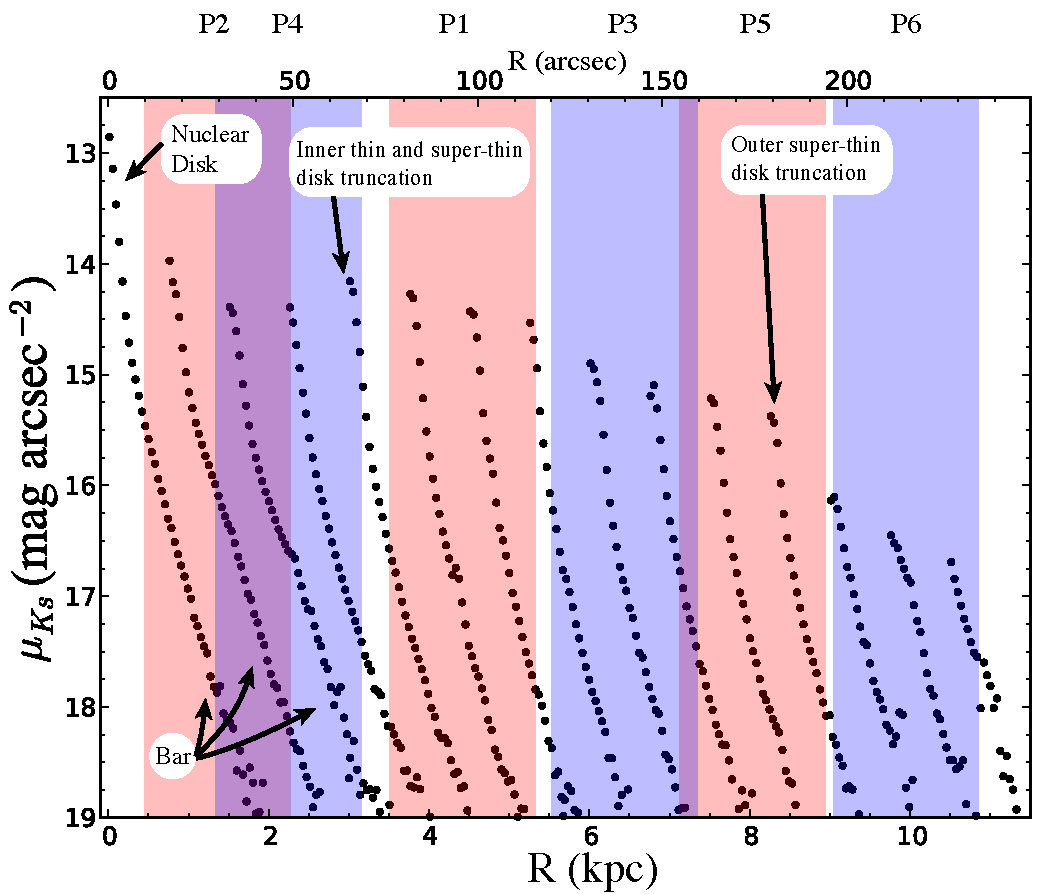
\includegraphics[width=0.8\columnwidth]{891_1/figs/ASR_pointings.pdf}
  \caption[\GP pointings compared to known features in NGC
  891]{\label{891_1:fig:ASR_comp}\fixspacing Comparison of our \GP pointings
    to attenuation-corrected K-band light profiles measured by
    \citet{Schechtman-Rook13}. Important morphological features from
    that work are labeled with arrows. Shaded regions show the radial
    extent of each \GP pointing. Positive values of radius (receding)
    are red and negative radius values (approaching) are blue. The
    innermost \GP pointings were chosen be within the inner disc
    truncation visible in the density profiles.}
\end{figure}

Figure \ref{891_1:fig:ASR_comp} shows our \GP pointings related to the
results of \citet{Schechtman-Rook13}, Figure \ref{891_1:fig:pointings}
contains a pointing map, and a summary of observations can be found in
Table \ref{891_1:tab:obslog}. Ideally we would have observed both the
southern vertical half of the extended disk as well as the northern
vertical half. However, our pointings cover the full inner
\val{0.5}{kpc} of the disk mid-plane in height and we anticipate
vertical asymmetries between the two half of the galaxy at larger
heights are modest compared to radial variations on the approaching
and receding sides.

\begin{figure*}
  \centering
  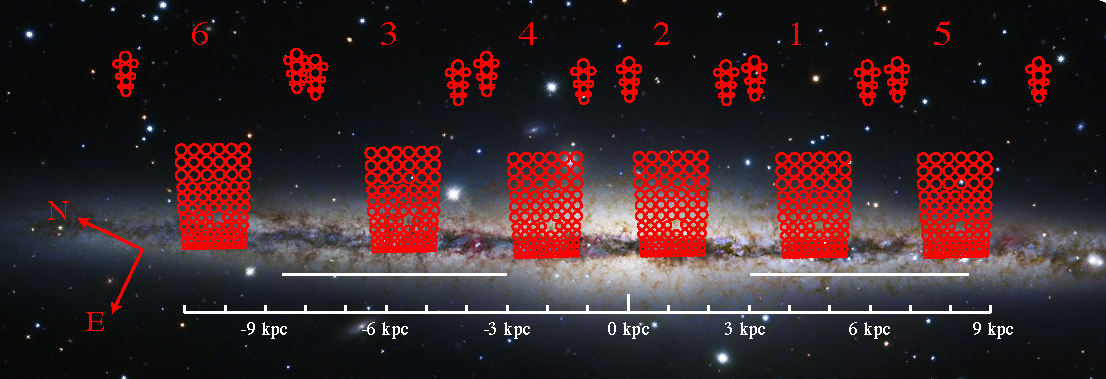
\includegraphics[width=\textwidth]{891_1/figs/NGC_891_better_pointings.pdf}
  \caption[NGC 891 \GP pointing map]{\label{891_1:fig:pointings}\fixspacing
    NGC 891 \GP pointings (Table \ref{891_1:tab:targets}) overlaid on
    combined Subaru (V band)/West Mountain Observatory (R,G,B)
    image. The horizontal white lines denote the extent of the
    super-thin disk reported by \citet{Schechtman-Rook13}. \emph{Image
      credit:} Robert Gendler, NAOJ, HST/NASA, BYU (Michael Joner,
    David Laney). In this orientation the approaching side is to the
    left.}
\end{figure*}

All individual exposures for NGC 891 were 30 min in duration. This
exposure time was chosen so that the dominant random error in the
measured counts is caused by photon shot-noise from the sky and galaxy
flux, and not detector read-noise. To further beat down the read-noise
all exposures were binned 2x2 before readout, which still allowed for
adequate sampling of the smallest fibers (\val{\asim 2}{pixels} full
width at half maximum in both the spectral and spatial
dimensions). The total integration time for each pointing varies with
radius and are based on the requirement of the MaNGA survey
\citep{Bundy15} to measure absorption line indices sensitive to age
and metallicity. This S/N limit is roughly 50 per resolution
element. In practice the complex structure of NGC 891 lowers this
limit, but, as shown in \S\ref{891_1:sec:snr_threshold}, a S/N of 50 is
larger than required for full-spectrum SSP fitting. Some extra time
left at the end of our program was used to increase the observation
time (and therefore S/N) of the outermost pointings (5 and 6) where
the signal was expected to be lowest.

For all \GP observations the PA offset was 295.79$^{\circ}$ (East of
North), which is slightly offset from perfectly perpendicular to the
disk of NGC 891. This offset allows each fiber to occupy a unique
location in $z$, but is small enough to not affect the differential
light-gathering power unique to \GP.

In all tables and future discussion in this paper and papers in this
series we define negative radii to be the NE side of NGC 891. This is
consistent with \citet{Oosterloo07}, who's HI data show that negative
radii correspond to the approaching side of the disk.

\subsection{Calibration Data}
\label{891_1:sec:cal_data}

In addition to on-sky galaxy exposures we took bias, dark, dome-flat,
CuAr arc lamp, and standard star exposures for use during data
reduction. Standard star and other calibration exposures were short
enough ($<\val{2}{min}$) that dark current was not a significant
source of noise for these frames. Unfortunately, for the longer
exposures the elevated dark current of the Lincoln Labs STA1 (SN 5644)
CCD currently used on the Bench requires accurate dark-frame
subtraction for any work approaching sky-limited surface-brightness
levels.  Dark frames were 30 minutes long (i.e., the length of a
single object exposure) and taken during the day, between nightly
observations.

Due to tight scheduling at WIYN we were only able to observe dome
flats and arc lamps at the beginning of each night. Comparisons
of these frames across nights (and even from month-to-month) show that
the Bench Spectrograph is stable following 30 minutes from a dewar
fill. Once-a-night calibration frames are adequate for accurate data
reduction so long as the spectrograph configuration is not changed.

The presence of multiple fiber sizes in \GP required modifications to
the standard calibration procedure for dome flats and standard
stars. In particular, two sets of dome flats at different exposures
are needed: one set with a short (\val{1}{sec.}) exposure time to
avoid saturating the largest fibers, and one set with a longer
(\val{4}{sec.}) exposure time to get enough signal in the smallest
fibers. These two sets are combined during data reduction as described
in \S\ref{891_1:sec:flats}.

Once during each of the observing runs a set of blank sky observations
was recorded during twilight (i.e., sky flats). Due to the challenging
nature of flat observations described above these flats were not
deemed suitable for use during data reduction, but we are optimistic
that further investigation and experimentation with sky flats can
yield success for future \GP programs.

Nightly observations were made of two standard stars taken from the
IDS Photometric Standards catalog, listed in Table \ref{891_1:tab:targets},
and were made \asim 2 times per star per night. The \GP fibers have a
broad range of sizes, which, at the smallest, are insufficient to
capture the entire PSF. Further, because of atmospheric refraction,
the amount of light lost in the smaller fibers varies with wavelength.
%% See Figure
%% \ref{fig:DAR} for an example of this effect and section
%% \ref{891_1:sec:flux_cal} for implications of this decision on our reduced
%% data.  
While scanning the stars across the fibers at the parallactic
angle would eliminate wavelength-dependent effects, the available
telescope software was not up to this task. Consequently, we chose to
use only the largest (5.62 arcsec diameter) fibers for standard star
observations. Each set of standard star observations used 2-4 fibers
so that over the course of the entire observing program all of the
5.62'' had been used to observe the standard stars. Application of
these observations to flux calibrating the NGC 891 observations is
described in \S\ref{891_1:sec:flux_cal}.

%% {\bf [TO DO: Explain how many different, large fibers were calibrated with
%%     standard-star exposures. See comments and give better description of
%%     Figure \ref{fig:DAR} if we decide to keep it or a modified version.]}

%% \begin{figure}
%%   \centering
%%   \includegraphics[width=\columnwidth]{figs/DAR.png}
%%   \caption{\label{fig:DAR} Standard star observed through multiple fiber
%%     sizes. For this observation \GP was dragged across the standard star to
%%     sample all 5 fiber sizes. The effects of DAR are clearly visible as the
%%     supression of the blue end of the spectrum in the 3” and 2” fibers (and a
%%     little bit in the 4” fibers). {\bf [TO DO for this figure: Decide if we
%%         want to include it. It might be better to show the ratio of these
%%         normalized spectra. Also wondering if we really want to get into these
%%         scans. I don't know if they were made at the same off-paralactic
%%         angle. Do you have this information? The reason to show a figure like
%%         this would be to demonstrate that our flux cal with the large fibers
%%         is likely not missing light in a wavelength differential sense. BIGGER
%%         LABELS]}}
%% \end{figure}

%% We attempted to reduce the effects of DAR in smaller fibers by dragging
%% the standard star across the IFU directly along the altitude axis, but found
%% that this did not provide substantial enough mitigation to warrent the added
%% time cost of such a procedure (\val{\sim 30}{min}).

%% Here we summarize the observing runs (number of nights, conditions),
%% spectrograph setup, objects, and positions per object. For the
%% spectrograph setup give the grating(s), grating angle ($\alpha$),
%% camera-collimator angle, central wavelength, dispersion, spectral
%% coverage and range of spectral resolution over the range of fibers
%% sizes.

%% Describe salient features of observations, such as calibration.  It is
%% worth mentioning need for dark frames.  Standard-star observations and
%% lessons learned from trying to drift vs using large fibers is
%% important to describe. The key point to mention is that we use the
%% largest fibers to eliminated DAR effects from the flux calibration. Do
%% we worry about telluric absorption over our observed range of
%% wavelengths, and if not what is the impact (what are the relative
%% strengths and wavelengths of the strongest features)? If we do worry
%% about telluric correction, how do we handle the varying spectral
%% resolution with fiber size?

%% Other calibration data, e.g., twilight flats?


\section{Data Reduction and Calibration}
\label{891_1:sec:data_reduction}

\subsection{Image processing and spectral extraction}

Basic reduction (overscan correction, bias/dark subtraction) were done
with IRAF's CCDPROC package. Cosmic rays were cleaned with the CRUTIL
package. Spectral extraction, wavelength calibration, and flux
calibration were done with the HYDRA package. The multiple fiber sizes
in \GP required modifications to the standard DOHYDRA procedure for
flat-field generation, sky-subtraction, and flux calibration. A
detailed walkthrough and discussion of these modifications can be
found at \url{www.astro.wisc.edu/~eigenbrot/GradPak}; we summarize the
important points below.

\subsubsection{Wavelength Calibration}
\label{891_1:sec:wavecal}

Uncertainties in the wavelength solution in the blue
($<$\val{4500}{\AA}) are the dominant source of uncertainty in
determining the line-of-sight doppler shift of the observed
spectra. As shown in Paper II, these velocities are important for
determining the line-of-sight depth of our spectroscopic observations,
which requires velocity precision better than the spectral resolution
of our data.
%% {\bf [QUESTION: for the purpose of velocities, why not
%%     just use the wavelengths longward of 4000? I think that would have
%%     been the right thing to do, but the broader point is that for
%%     doing chi$^2$ analysis down to H\&K we need wave calibration
%%     better than the spectral resolution. This is a point we echo in
%%     the last section on the instrumental dispersion so important to
%%     point it out here too: we need accurate first and second
%%     moments.]} 
The reason for the wavelength calibration uncertainty
at short wavelengths is the combined dearth of strong spectral
features in the CuAr arc-lamp and the sensitivity fall-off in the
fibers, spectrograph optics, grating and CCD. The number of good
spectral lines that can be fit from the available arc-lamps between
\val{4130}{\AA} and \val{7300}{\AA} is 33.

To characterize the uncertainties in the wavelength calibration, we
measure the centers of Solar Ca H\&K absorption (from zodiacal or
atmospheric scattering) and three HgI emission lines (atmospheric
scattering from terrestrial sources, e.g., Tucson) in our data before
sky subtraction. In all of our data exposures the foreground (zodiacal
plus atmospheric) signal dominated over the flux from NGC 891 to the
point where discrimination between Solar Ca H\&K and Ca H\&K in NGC
891 was not necessary.

For each night of observation all wavelength-calibrated object frames
are combined to improve S/N (especially relevant for measurements of
absorption lines) before line centroids are measured with IRAF's
FITPROFS routine. For each line measured the average offset from the
known center across all \GP fibers is taken as an indication of the
accuracy of the wavelength solution at that particular wavelength. The
standard deviation of the measured centers across all \GP fibers is a
measure of the precision of the wavelength solution at a particular
wavelength.

\begin{figure}
  \centering
  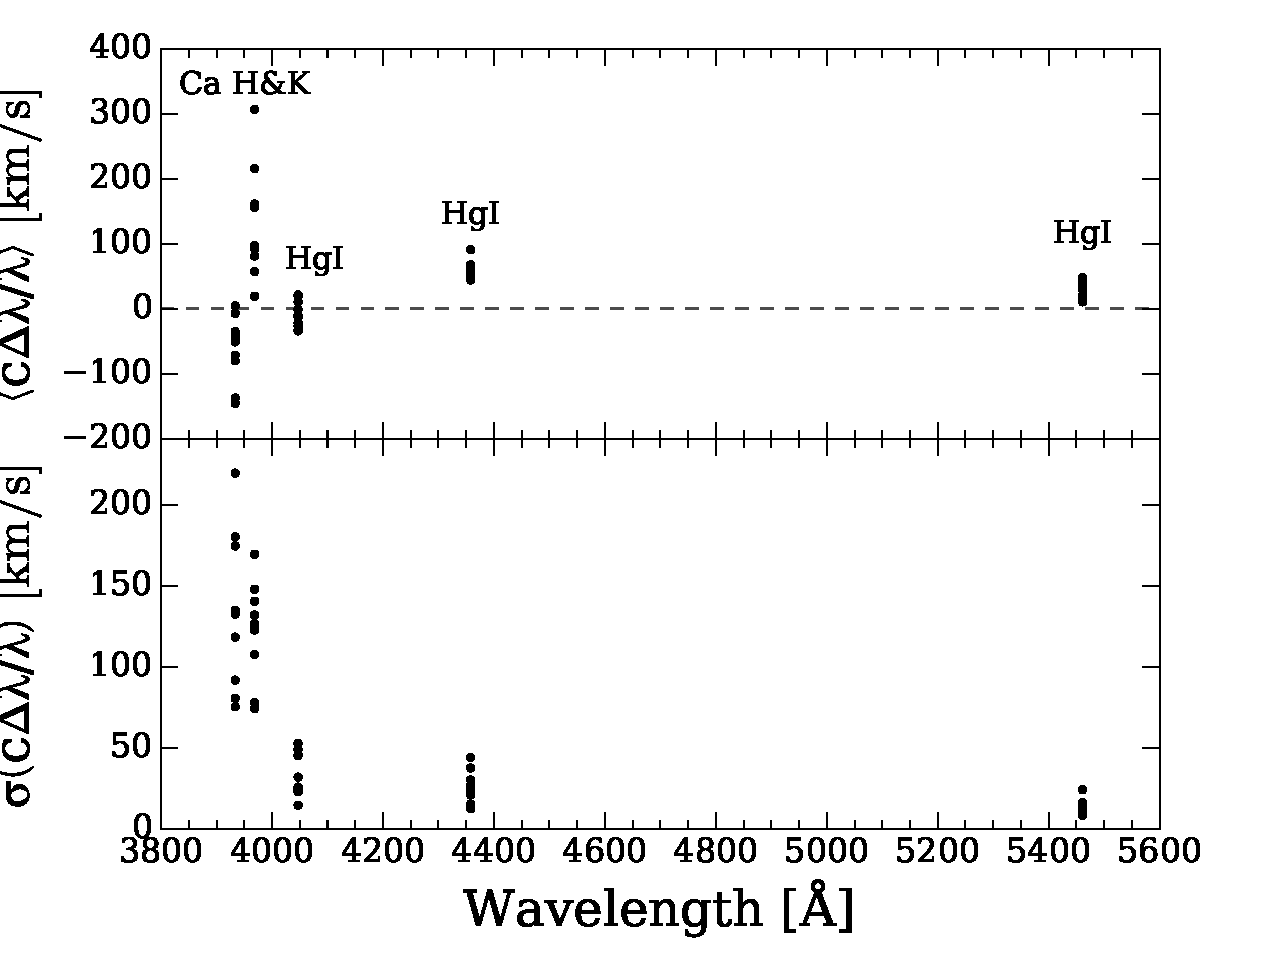
\includegraphics[width=\columnwidth]{891_1/figs/Wave_Err_comb.pdf}
  \caption[Accuracy and precision of wavelength
  calibration]{\label{891_1:fig:wave_err}\fixspacing Estimated accuracy and
    precision of the wavelength solution in the blue region of the
    spectrum based on measurements of known foreground features (HgI
    emission at 4047, 4358 and 5461 \AA\ from terrestrial light
    pollution, and Solar Fraunhofer H\&K lines from Ca) in our sky
    spectra.  Each point corresponds to a measurement of a line from
    an individual night of NGC 891 observations. \emph{top:} The mean
    offset in km $^{-1}$ between measured line centers and the known
    values, averaged over all \GP fibers. \emph{bottom:} The standard
    deviation of the measured line centers in km s$^{-1}$, computed
    across all \GP fibers.}
\end{figure}

Accordingly, Figure \ref{891_1:fig:wave_err} shows the estimated accuracy
and precision for each of the 10 nights of NGC 891 observations.  At
wavelengths $>\val{\asim 4000}{\AA}$ our wavelength solution is both
accurate and precise to within \val{\asim 50}{\kms}. Below
\val{4000}{\AA} (where the wavelength solution is determined via
extrapolation of the CuAr lamp line data) we measure a systematic
offset of \val{\asim 120}{\kms} with a comparable value for the random
error. We therefore report an upper limit on the uncertainty in our
wavelength solution to be \val{120}{\kms} at \val{4000}{\AA}, while
noting that for most wavelengths this is an overestimation.  The RMS
uncertainty reported by the wavelength fitting routine is \val{\asim
  90}{\kms}, which is likely a more accurate estimate of the
uncertainty for the wavelength region covered by arc lines
(\val{4130}{\AA}$<\lambda <$ \val{7300}{\AA}).  Even in the worst case
we are able to calibrate wavelengths to a higher precision than the
spectral resolution (see \S\ref{891_1:sec:GPak_dispersion}), which varies
from 180 to \val{570}{\kms} at \val{4000}{\AA} (depending on fiber
size). Thus, accurate measurements of velocity based on $\chi^2$
fitting of absorption lines (as done in Paper II) is possible with our
data.


%% The maximum offset from the true values give us an
%% upper limit on the uncertainty in our wavelength solution. Using this
%% method we find an upper limit of \val{\asim 100}{\kms} at
%% \val{4000}{\AA}, which is consistent with the value of \val{\asim
%%   90}{\kms} based on the RMS of the wavelength solution fit. {\bf
%%   [TODO: Let me get this straight: we are not using these features to
%%     improve the calibration, but just as a cross-check?]}

\begin{figure}
  \centering
  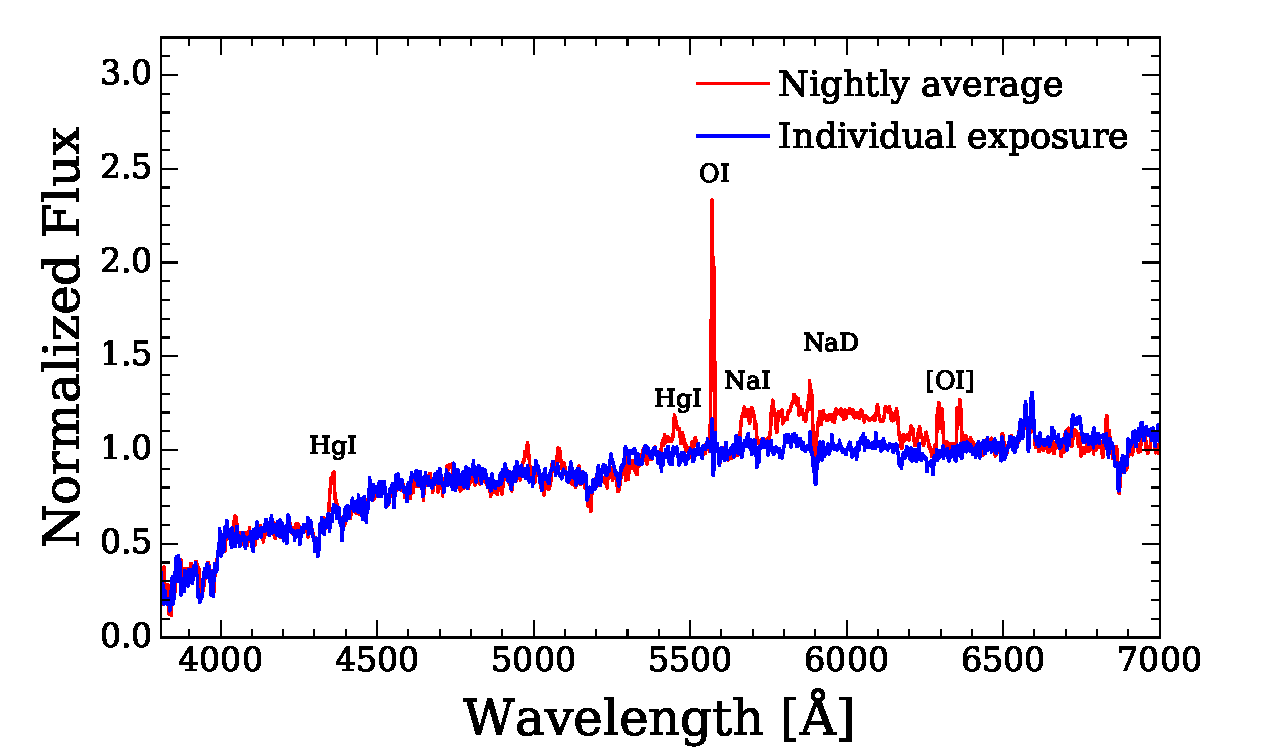
\includegraphics[width=\columnwidth]{891_1/figs/skysub_comp.pdf}
  \caption[Sky subtraction example]{\label{891_1:fig:skysub_comp}\fixspacing Example of large
    sky-subtraction residuals from November 21st, 2014. The red
    spectrum shows fiber 80 after sky subtraction using a sky spectrum
    that is the average across the whole night. The blue spectrum
    shows the same fiber using after sky subtraction using only the
    sky fibers from the same exposure. The large residuals around
    \val{6000}{\AA} (a broad high-pressure sodium feature) have been
    eliminated along with a number of strong, narrow emission lines.}
\end{figure}

\subsubsection{Flat Fields}
\label{891_1:sec:flats}

The combination of spectrograph setup and the multiple fiber sizes in
\GP required two different dome flat exposure times: a short exposure
(\val{1}{s}) to avoid saturating the largest fibers, and a long
exposure (\val{4}{s}) to get adequate signal in the smallest fibers.
%% Repeat
%  For this reason we took one set of \val{4}{s} dome flats to produce
% enough signal in the smallest fibers (while saturating the largest
% fibers) and one set of \val{1}{s} dome flats to avoid saturating the
% largest fibers (while getting almost no signal in the smallest
% fibers).
Both sets of dome flat exposures were run through CCDPROC, combined,
and had their apertures extracted independently by DOHYDRA.  The
so-called ``extraction'' produces a one-dimensional data vector
(spectrum) for each fiber. In both cases the extraction used fiber
traces computed from the \val{1}{s} flat for all data because we found
that saturated large fibers in the \val{4}{s} flats introduced errors
in the extraction process while the low signal in small fibers at
\val{1}{s} was still adequate for tracing purposes. In practice,
traces using the \val{4}{s} or \val{1}{s} are very similar, as
confirmed with the intermediate-size fibers that have good signal
without being saturated. This is expected given the fact that the two
exposure sets were taken right after each other over a short period of
time.

Once the two flats had their apertures extracted, the resulting
spectra were scaled to the same exposure time and stitched together
into a ``master'' flat where the 1\farcs87 and 2\farcs81 fibers were
taken from the \val{4}{s} flat and the 3\farcs75, 4\farcs69, and
5\farcs62 fibers were taken from the \val{1}{s} flat. This master flat
was used in all subsequent reduction of the on-sky data.

During the exercise of establishing this pipeline we discovered a lag
in the shutter time that affects exposures shorter than \val{\asim
  7}{s}. The WIYN Bench Spectrograph CCD has a linear slide shutter
that has opening and closing times that are not equal. Because the
shutter moves along the wavelength dimension of the CCD the effect of
this inequality is to add an artificial spectral signature. The
magnitude of this signature varies with exposure time, with the
largest deviation measured as $\asim 20\%$ at \val{1}{s}. We removed
this spectral mismatch between the \val{1}{s} and \val{4}{s} flats by
normalizing all fibers in the \val{4}{s} flat to the mean spectrum of
the \val{1}{s} flat. While this method still introduces the shutter
spectrum present in the \val{4}{s} flat this spectrum is constant
across all fibers and is thus removed during flux calibration.

\subsubsection{Sky Subtraction}
\label{891_1:sec:skysub}

Each fiber size in \GP has 4 dedicated sky fibers, as illustrated in
Figure \ref{891_1:fig:GradPak}.  Sky subtraction was performed on a
fiber-size basis using different beam numbers for each fiber size in
HYDRA's SKYSUB routine.  Since there are multiple sky fibers rejection
of contaminated sky fibers was possible, as indeed was required (see
Figure \ref{891_1:fig:pointings} for P6, P4, P1).

The data from the night of November 21st, 2014 (P1) showed strong
variation in sky intensity across the course of the night. This
variation did not subtract well when using a sky spectrum averaged
across the whole night. In particular, the region between atmospheric
NaI emission at \val{5684}{\AA} and the broad high-pressure sodium
feature around \val{5900}{\AA} often left strong residuals when using
a nightly average for the sky spectrum. Accurate sky subtraction was
achieved by computing the average sky spectrum on an
exposure-by-exposure basis and combining individual object exposures
\emph{after} sky subtraction. For consistency across the observing
program the data for all nights was sky subtracted in this way. Figure
\ref{891_1:fig:skysub_comp} shows representative before-and-after spectra
illustrating this issue.

\begin{figure}
  \centering
  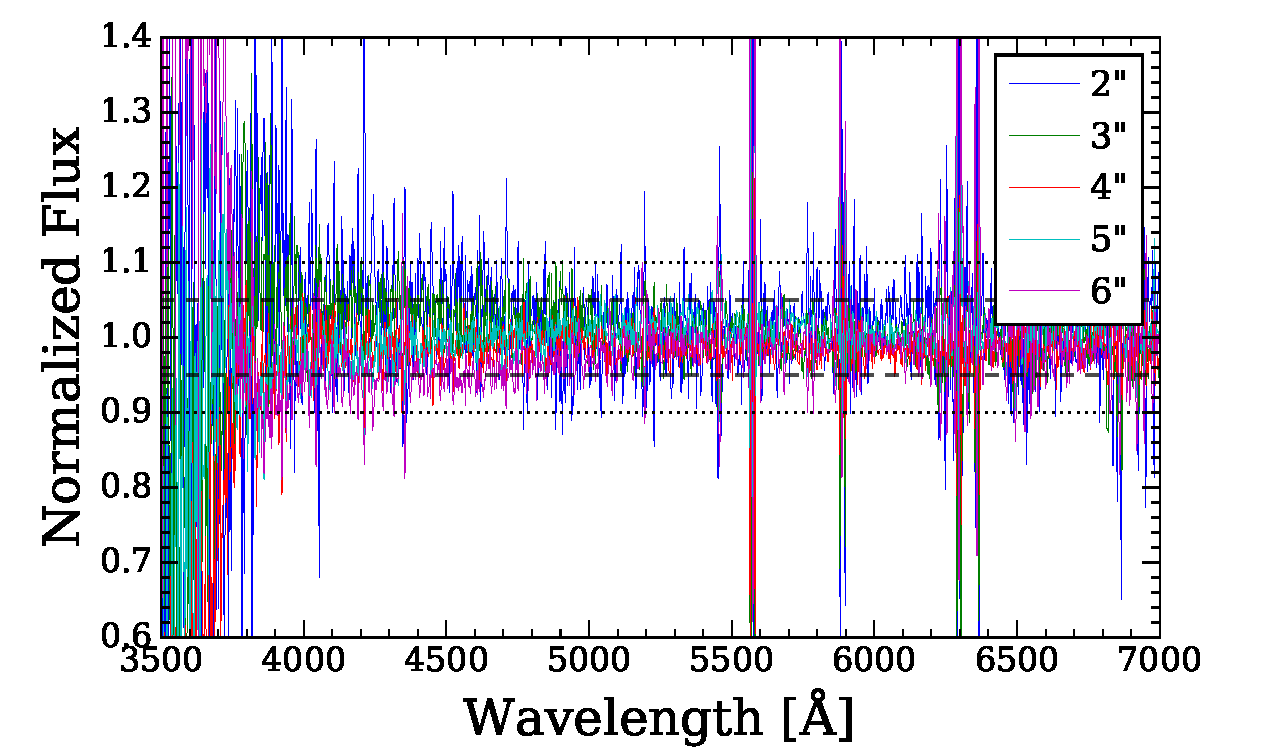
\includegraphics[width=\columnwidth]{891_1/figs/flux_cal_test.pdf}
  \caption[Comparison of flux calibration across multiple fiber
    sizes]{ \label{891_1:fig:sky_flux_comp}\fixspacing Flux
    calibration test for all fiber sizes when using standard star data
    from only 5\farcs62 fibers. Data are taken from a single galaxy
    exposure reduced through flux calibration, but not
    sky-subtracted. Each line represents the average of all 4 sky
    fibers for a given fiber size and all lines are normalized by the
    mean of all sky fibers. The dashed and dotted lines show
    deviations at the 5\% and 10\% level, respectively. All fiber
    sizes show an absolute flux calibration consistent within 5\% for
    wavelengths $>$ \val{4000}{\AA}. At \val{4000}{\AA} the 2 arcsec
    and 3 arcsec fibers deviate by up to 20\%.}
\end{figure}

\subsection{Flux Calibration}
\label{891_1:sec:flux_cal}

%% {\bf [TO DO: There is basic argument that we need to make for why we
%%     think application of the flux cal from the large fibers to all
%%     fibers is valid. This consists of a combination of the fact that
%%     all of the fiber is of the same material. However, beause it is
%%     not necessarily from the same draw, there could be
%%     variations. That is where information from lab measurements in the
%%     \GP instrument description section would be useful.]} 

As discussed in \S\ref{891_1:sec:cal_data} atmospheric refraction limited
our standard star observations to only the 5\farcs62 fibers. On each
night the same two standard stars were observed in multiple 5\farcs62
fibers and a flux calibration was computed using the ONEDSPEC
package. Time constraints in our observing program limited the range
of airmasses available for standard star observations and for this
reason we could not compute an extinction curve for our data. We
instead used the KPNO extinction curve provided in
ONEDSTDS\footnote{http://stsdas.stsci.edu/cgi-bin/gethelp.cgi?onedstds}.

\begin{figure}
  \centering
  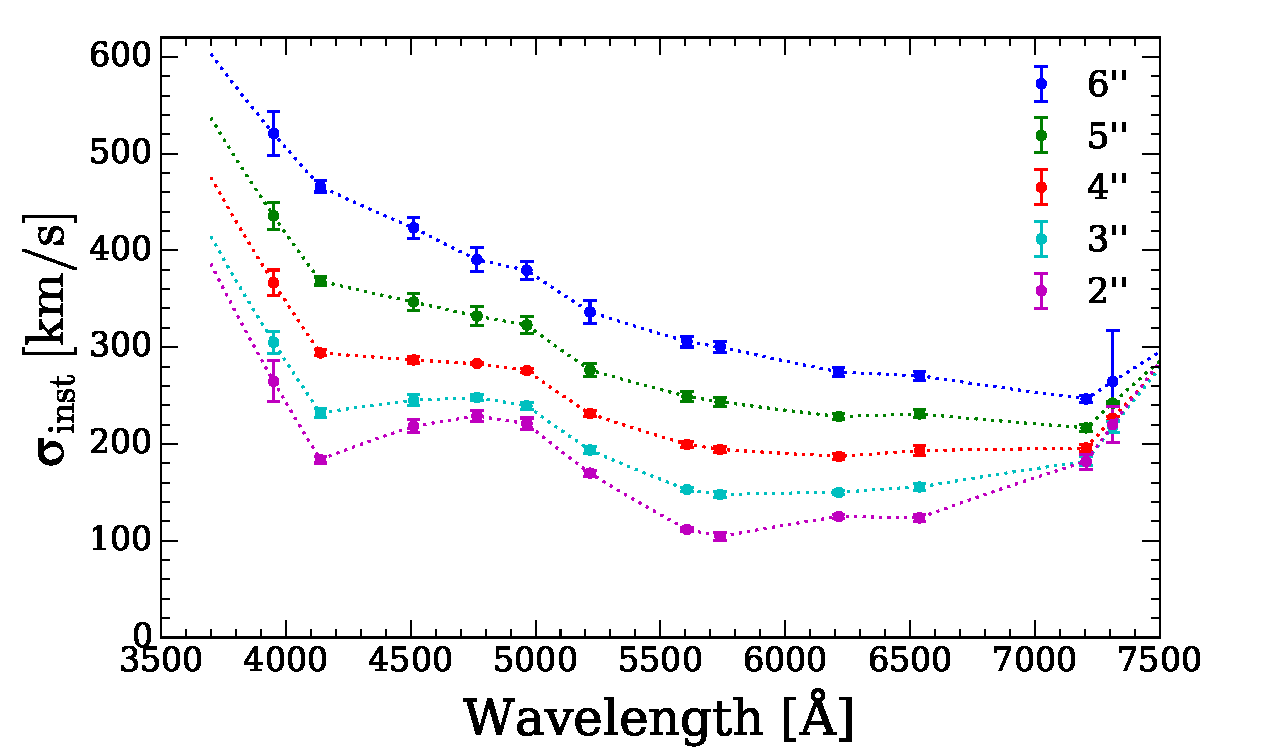
\includegraphics[width=\columnwidth]{891_1/figs/disp_paper.pdf}

  \caption[Variation of instrumental resolution in \GP
  fibers]{\label{891_1:fig:dispfunc}\fixspacing Instrumental resolution as
    measured from CuAr arc-lamps (see text) are plotted as points; the
    interpolated and extrapolated dispersion functions used in
    spectral modeling is shown by the dotted lines.}
\end{figure}

To zeroth order we expect the spectral response of all the \GP fibers
to be the same because they are made of the same material and are all
from the same foundry run \citep{Wood12}. In reality the \GP fibers
come from different draws, were handled differently during
construction, and have different degrees of termination quality.
Consequently, there are throughput variations not only between fiber
sizes, but also within fiber sizes, as illustrated in Figure
\ref{GPtesting:fig:TL_FRD}.  Throughput characteristics vary across the \GP
array. In particular, the total throughput and focal ratio degradation
are worse for the smallest fibers. The throughput variations are
expected to relatively grey (wavelength independent), but since there
are variations in FRD, this can lead to different, wave-length
dependent losses within the spectrograph. Since the flat-field screen
uniformly illuminates the array, the flat-fielding process should
remove all of these relative variations.

To assess the effects of using flux standards taken in a single fiber
size to calibrate the entire \GP IFU we compared flux calibrated sky
spectra for all fiber sizes. The data came from a single exposure of
P3 (see Figure \ref{891_1:fig:pointings}) where none of they sky spectra
appeared to be outliers due to source contamination from foreground
stars or background galaxies.  All sky fibers were flux calibrated
using data from the 5\farcs62 fibers, and then the 4 sky fibers of each
size were averaged together. Figure \ref{891_1:fig:sky_flux_comp} shows the
average spectrum for each fiber size, normalized to the mean of
\emph{all} sky fibers. At wavelengths greater than \val{4000}{\AA} the
sky spectra are consistent between fiber sizes to within 5\%. Below
\val{4000}{\AA} the flux calibration varies by up to $\asim$20\% due
to low signal to noise at these wavelengths.

%% {\bf Here's what MAB doesn't understand: (a) why do the
%%   strong sky lines, like OI at 5563 or so, show such large variations?
%%   (b) you say the flux cal varies a lot below 4000A due to low SNR in
%%   the smallest fibers yet the magenta curve for the 6'' fibers seems
%%   as aberrant as any.}

To account for night-to-night offsets in extinction (caused by, e.g.,
high cirrus clouds) we scaled each individual exposure so that all
exposures in a particular pointing have the same average flux in the
region $\val{4500}{\AA} \leq \lambda \leq \val{5500}{\AA}$. Within a
single night this scaling was always less than \asim 3\%, but between
nights it could vary by a factor of up to 2 in cases where a night had
poor observation conditions (high humidity, persistent clouds,
etc.). The final spectra for each pointing are an average of
individual exposures weighted by the square of the inverse of their
deviation from the mean pointing flux in the range $\val{4500}{\AA}
\leq \lambda \leq \val{5500}{\AA}$.

\subsection{Instrumental Line Profile}
\label{891_1:sec:GPak_dispersion}

The optical distortions of the WIYN Bench Spectrograph result in an
instrumental line profile that varies with wavelength and field
location along the fiber slit for a fiber of a given size. The
delivered line profile in the spectral dimension (the instrumental
dispersion) is a convolution of this distortion with the
anamorphically demagnified fiber image. Consequently the different
fiber sizes in \GP cause the spectral line profile to be a different
function of wavelength for each fiber size. We refer to this value as
$\sigma_{\rm inst}$, reported in units of \kms.

To account for the variations in $\sigma_{\rm inst}$ in our later
fitting of model spectral energy distributions, we first measured the
width of arc-lamp emission lines across our entire wavelength range
for all fibers. Widths for each arc line were measured for every
fiber, and then averaged for all fibers of the same size, weighted by
poisson noise in each fiber. Arc lines with low signal-to-noise were
combined together in groups over narrow wavelength ranges to improve
the signal and assigned a new wavelength weighted by the
signal-to-noise of the component lines. This was particularly
important in the far blue where the lines were few and often
weak.

These data were interpolated to create dispersion functions,
$\sigma_{{\rm inst},i}(\lambda)$, for each fiber size, $i$. Past the
blue and red ends of the region covered by arc lines
(\val{4130}{\AA}$<\lambda <$ \val{7300}{\AA}) the dispersion functions
are extended with linear extrapolation. The line-width data and
resulting instrumental dispersion functions can be found in Figure
\ref{891_1:fig:dispfunc}. Note the hat-shaped profile seen for the smallest
fibers, characteristic of the typical compromise focus value chosen
for the all refractive Bench Spectrograph system. For larger fiber
sizes the resolution is dominated by the geometric fiber diameter and
the changes in the grating dispersion with wavelength.




\section{Signal to Noise and Spatial Binning}
\label{891_1:sec:maps}

\begin{figure}
  \centering
  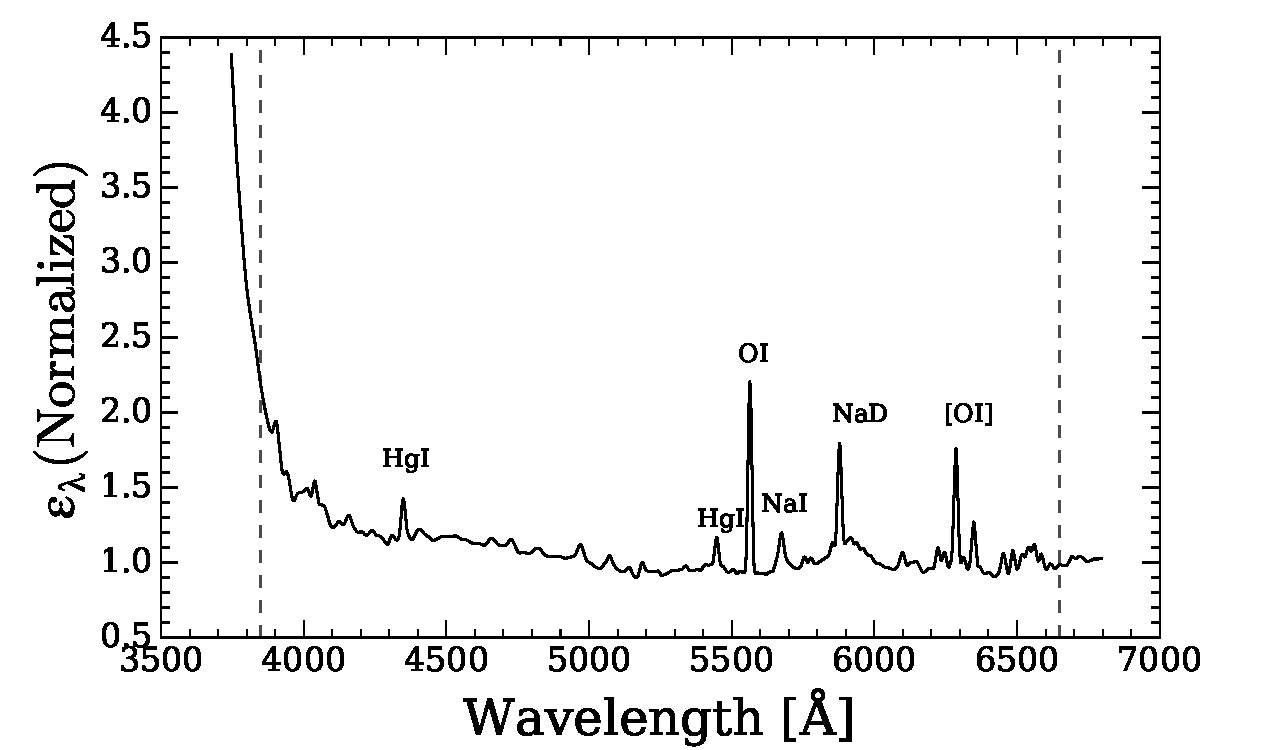
\includegraphics[width=\columnwidth]{891_1/figs/noise_vec.pdf}
  \caption[Characteristic noise
  spectrum]{\label{891_1:fig:noise_vec}\fixspacing Characteristic noise
    vector used to construct noisy galaxy models, as described in the
    text, here normalized between \val{5450}{\AA} $\leq \lambda \leq$
    \val{5550}{\AA}. Vertical dashed lines correspond to used spectral
    range in analysis.}
\end{figure}

\subsection{Signal-to-Noise threshold for spectral bins}
\label{891_1:sec:snr_threshold}

Despite \GP's design, clumpiness in the distribution of dust and
star-light result in different signal-to-noise ratios (S/N) in each
fiber. Co-adding spectra (``binning'') from adjacent fibers enables us
to homogenize S/N and hence the precision on age and metallicity
inferred from spectral fitting, but at the expense of spatial
resolution. We have attempted to optimize the spectral binning by
defining a critical S/N threshold to achieve a {\it precision} of 10\%
in age and metallicity. In the absence of other mitigating effects,
this precision is ample to detect the vertical age break in a MW-like
heating model and to determine the break height to within 50 pc since
the predicted gradient in light-weighted mean age is very steep near
the mid-plane. At this level of precision, systematic effects in the
interpretation of the break height, e.g., due to inaccuracies of our
estimated line-of-sight depth or model assumptions about star-forming
history become dominant. In what follows we define S/N in pixel units,
where each pixel samples roughly 2\AA.

Accordingly, the critical S/N threshold was determined using an
idealized Monte Carlo simulation of model galaxy spectral energy
distributions (SED) with known star formation histories and
chemistries and therefore known ages and metallicities.  We have
ignored systematic errors in, e.g., flux calibration or between the
model libraries and stellar evolutionary tracks and actuality,
although we address issues with stellar libraries and evolutionary
tracks in Paper II. While other studies have undertaken similar
analyses we stress the importance of this modeling exercise to be
undertaken to any data set distinct in wavelength range and error
vector.

\begin{figure}
  \centering
  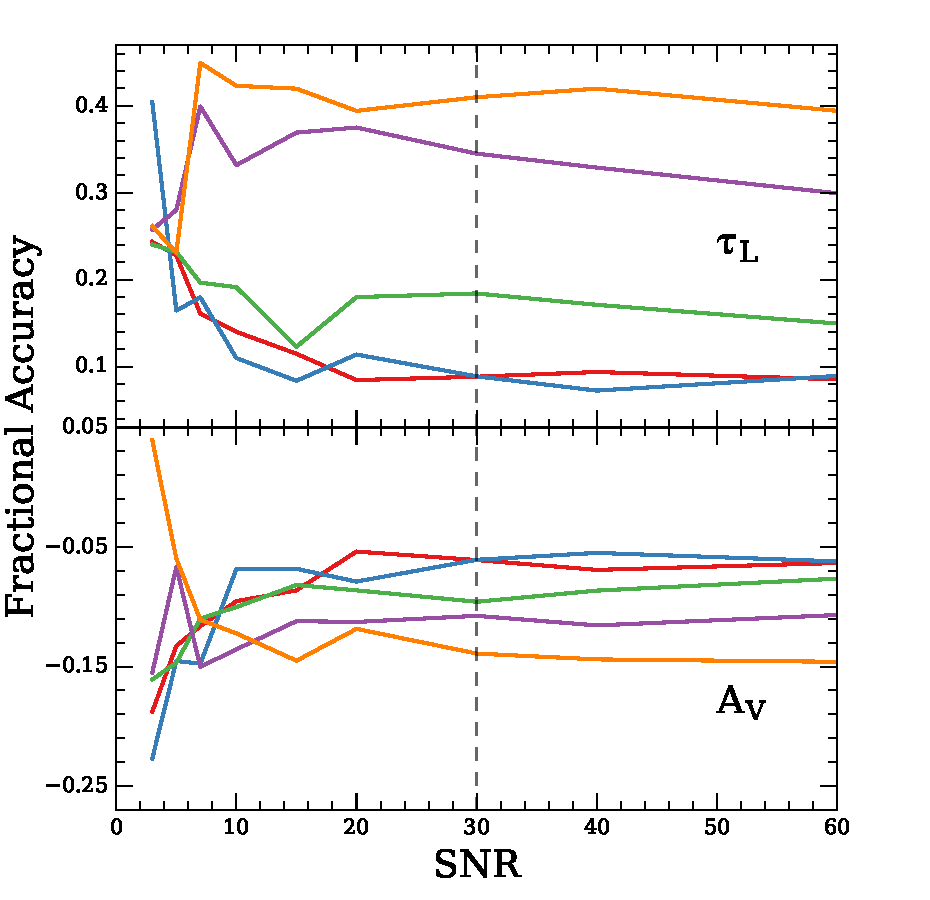
\includegraphics[width=\columnwidth]{891_1/figs/SN_sys.pdf}

  \caption[Systematics in model galaxies used for S/N
  determination]{\label{891_1:fig:SN_sys}\fixspacing Systematics in fit
    parameters caused by degeneracies in star formation history as a
    function of S/N per pixel (each pixel samples $\sim 2$\AA).
    Fractional accuracy is defined as $1 -
    X_\mathrm{fit}/X_\mathrm{model}$, where $X = \tau_L$ in the top
    panel, and $X = A_V$ in the bottom panel.  Models adopt a
    solar-metallicity smoothly declining star-formation rate governed
    by an e-folding time-scale $\tau_{SF}$, while the fit has no
    restrictions on the SFH or metallicity. Colors correspond to
    different values of $\tau_{SF}$ as given in Figure
    \ref{891_1:fig:SN_rms}. Vertical dashed lines at S/N=30 pix$^{-1}$) are
    for reference.}
\end{figure}


\begin{figure}
  \centering
  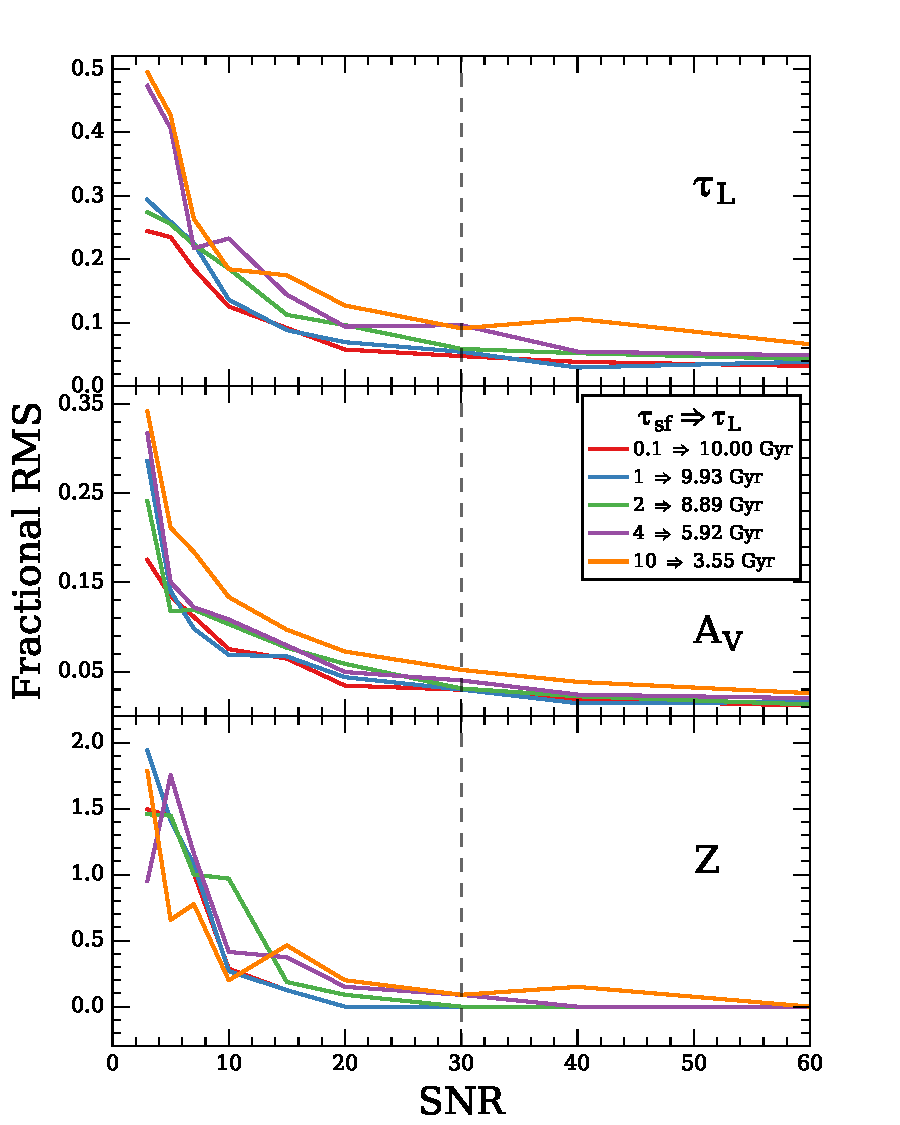
\includegraphics[width=\columnwidth]{891_1/figs/SN_rms.pdf}
  \caption[Precision of derived parameters as a function of
  S/N]{\label{891_1:fig:SN_rms}\fixspacing Precision of recovered parameters
    as a fraction of S/N per pixel for different model input values of
    mean light-weighted age ($\tau_L$, top), extinction ($A_V$,
    middle), and metallicity ($Z$, bottom).  Precision is estimated as
    the root-mean-square deviation of the fitted values from the mean
    of the 30 Monte Carlo noise realizations. Colored lines correspond
    to results for model spectra described in Figure \ref{891_1:fig:SN_sys},
    as indicate in the key. Model values of $\tau_L$ for each
    $\tau_{SF}$ assuming a formation epoch 12 Gyr in the past are also
    specified. Vertical dashed lines at S/N = 30 pix$^{-1}$ indicate
    our precision criterion largely driven by $\tau_L$.}
\end{figure}

\subsection{Monte Carlo Simulations}
\label{891_1:sec:sims}

Model galaxy spectra were constructed using the method outlined in
Appendix \ref{891_1:sec:tau_model} with star-formation e-folding
time-scales, $\tau_{SF}$ = 0.1, 1, 2, 4, and 10 Gyr for a total age of
12 Gyr.  All model galaxies were constructed from mono-metallicity
SSPs with a metallicity of \val{0.4}{\Zsol} and had extinction
dictated by the model of \citet{Charlot00} with $A_V=1.63$ (an optical
depth $\tau_V$ of 1.5, close to the median we in in Paper II from full
spectral fitting). The spectral resolution of the models was set to
210 km s${^-1}$ to match the characteristic resolution of the data at
5500 \AA. For each model galaxy noise was added to produce spectra
with S/N = 3, 5, 7, 10, 15, 20, 30, 40, and 60. We define S/N for both
our galaxy observations and Monte Carlo models as S/N =
$\Sigma_{\lambda}\left(f_\lambda/\epsilon_\lambda\right)/N$ where
$f_\lambda$ is the measured flux, $\epsilon_\lambda$ is the
corresponding error vector, and the sum is over $N$ pixels in a
specified band pass. For our tests we choose the bandpass to be
\val{5450}{\AA} $\leq \lambda \leq$ \val{5550}{\AA}, but we note that
the choice of bandpass only scales the derived S/N thresholds by a
constant related to the SED of our galaxy/models. Provided the
bandpass used to compute the S/N threshold is the same as that used to
bin the data the specific choice of bandpass is irrelevant.

For observed galaxy data the quantities $f_\lambda$ and
$\epsilon_\lambda$ are the result of the reduction described in
section \ref{891_1:sec:data_reduction}. For the model galaxies the shape of
$\epsilon_\lambda$ was based on the spectral noise structure of our
data.  To compute $\epsilon_\lambda$ we average together the error
vectors from \emph{all} fibers across all pointings. We then fit a
smooth function to this average to remove high-frequency noise. The
result in Figure \ref{891_1:fig:noise_vec} captures the general trend of how
$\epsilon_\lambda$ varies with wavelength in our data.

% {\bf [TODO: A little more discussion and description in the next paragraph 
% is needed. 

% A few things to discuss include:

% Can we say why we think it is reasonable to fit mono-z templates to
% the mono-z simulations? I am thinking about the fact that ultimately
% we expect there to be multi-z stellar pops in N891 and that
% regardless, in the end we fit multi-z models to the data. Do we want
% to know what happens when we allow this degree of freedom in the
% simulations? Will we want to know it when we get back to Paper II?

% Discuss why we are not forcing the fit to have exp SFR, or do we want
% to do that as well? Are we showing anything about this in Paper II? 

For each combination of $\tau_{SF}$ and S/N we generate 30 Monte Carlo
noise realizations (while still maintaining the same S/N) which
produce 30 version of the same galaxy that differ only by stochastic
variations. Once the model galaxies are constructed they are fit using
the same method described in Paper II. In short, a Levenberg-Marquardt
minimization routine is used to fit a superposition of SSPs taken from
the models of \citet{Bruzual03} in the same 10 age bins used by
\citet{Tremonti04} (in Gyr: 0.005, 0.025, 0.1, 0.286, 0.64, 0.904,
1.434.2.5, 5, and 10). The result of each fit is a set of SSP weights
and a single value for extinction $A_V$, assuming the extinction model
of \citet{Charlot00} (i.e., the same extinction model used to
construct the model galaxies). In both the models and the fitting, we
have made the simplifying condition that the same value for the
extinction and the extinction law is applicable to all age stellar
populations; to do otherwise is beyond the scope of this analysis.

When assessing the accuracy and precision of each S/N level we
directly compare the known model $A_V$ to the fit $A_V$, and we use
the mean light-weighted age ($\tau_L$, Equation \ref{TM:eq:MLWA} in
Appendix \ref{chap:tau_model}, as measured between \val{5450}{\AA}
$\leq\lambda\leq$ \val{5550}{\AA})\footnote{ This band-pass for
  defining $\tau_L$ is between and narrowly missing terrestrial and
  airglow lines of HgI and OI. However, since the measurement is made
  from and referenced to the models, night-sky contamination is not
  relevant.}  as a proxy for the SSP weights. This substitution allows
us make a quantitative assessment of the {\it precision} of our fits
but comes with some important caveats concerning {\it accuracy} that
we consider in detail in Paper II, and summarize here.

In the broadest terms $\tau_L$ is known to be degenerate with the
detailed star formation history (SFH); in our models we assume a
smooth, exponentially declining star-formation rate parameterized by
$\tau_{SF}$ but a different SFH could yield a very similar spectrum
with a significantly different $\tau_L$.  Because we do not impose a
specific SFH during the fitting process, our fit values of $\tau_L$
are likely to be systematically offset from the input model values.

More specifically, we find that any model with a smoothly varying
prescription of the SFH (specifically the $\tau_{SF}$ model outlined
in Appendix \ref{chap:tau_model}) gives a generally poor description of
our galaxy spectra and also yield estimates of SFH (via $\tau_L$) that
are offset from the best fitting models with unconstrained star
formation histories. We highlight these systematics in Figure
\ref{891_1:fig:SN_sys}.

Fits with unconstrained SFH report values of $\tau_L$ that are offset
by as much as 40\% from the true values of $\tau_{SF}$ model
galaxies. The maximum offsets occur at the largest values of
$\tau_{SF}$, i.e., approaching a constant star-formation rate where
all age SSPs are well represented in the integrated spectrum.  This
suggests systematics may be driven by degeneracies caused by
similarities between the 10 SSPs used during fitting.  In Paper II we
explore methods to reduce the number of SSPs used (and therefore the
number of free parameters) using the statistical methods presented by
\citet{Mosby15}.

\begin{deluxetable}{cccrrrc}
\tablewidth{0.8\textwidth}
\tablecaption{Data Apertures}
\tablehead{
\colhead{Pointing} &
\colhead{Aperture} &
\colhead{Constituent} &
\colhead{S/N} &
\colhead{$r$} &
\colhead{$z$} &
\colhead{Notes}\\
\colhead{Number} &
\colhead{Number} &
\colhead{Fibers} &
\colhead{} &
\colhead{(kpc)} &
\colhead{(kpc)} &
\colhead{}
}
\startdata
1 & 1 & 3, 4, 5, 6, 7, 8 & 32.22 &  4.44 & -0.12 & g\\
1 & 2 & 9, 10, 11, 12, 13, 14, 15, 16, 17 & 26.72 &  5.26 & -0.09 & b\\
1 & 3 & 21 & 34.50 &  4.16 &  0.02 & g\\
1 & 4 & 22, 23, 24, 25, 26, 27 & 31.41 &  4.76 &  0.04 & g\\
1 & 5 & 28, 29, 30 & 14.92 &  5.52 &  0.08 & u\\
1 & 6 & 33, 34, 35, 36, 37, 38, 39 & 30.70 &  4.66 &  0.21 & g
  %% 1 & 7 & 40, 41, 42 & 15.89 &  5.51 &  0.24 & g\\
  %% 1 & 8 & 45, 46, 47, 48 & 30.85 &  4.47 &  0.41 & g\\
  %% 1 & 9 & 49, 50, 51 & 47.30 &  5.24 &  0.44 & g\\
  %% 1 & 10 & 52 & 32.77 &  5.68 &  0.46 & g\\
  %% 1 & 11 & 55, 56, 57, 58, 59 & 43.21 &  4.61 &  0.63 & g\\
  %% 1 & 12 & 60 & 40.73 &  5.45 &  0.67 & g\\
  %% 1 & 13 & 61 & 36.45 &  5.67 &  0.68 & g\\
  %% 1 & 14 & 64, 65 & 48.93 &  4.22 &  0.87 & g\\
  %% 1 & 15 & 66 & 43.20 &  4.62 &  0.89 & g\\
  %% 1 & 16 & 67 & 37.63 &  4.89 &  0.90 & g\\
  %% 1 & 17 & 68 & 39.57 &  5.16 &  0.91 & g\\
  %% 1 & 18 & 69 & 35.57 &  5.43 &  0.92 & g\\
  %% 1 & 19 & 70 & 32.84 &  5.69 &  0.94 & g\\
  %% 1 & 20 & 72 & 36.81 &  4.07 &  1.13 & g\\
  %% 1 & 21 & 73 & 48.06 &  4.34 &  1.15 & g\\
  %% 1 & 22 & 74 & 40.16 &  4.61 &  1.16 & g\\
  %% 1 & 23 & 75 & 39.75 &  4.88 &  1.17 & g\\
  %% 1 & 24 & 76 & 30.52 &  5.15 &  1.18 & g\\
  %% 1 & 25 & 77, 78 & 28.73 &  5.55 &  1.20 & g\\
  %% 1 & 26 & 80 & 41.76 &  4.06 &  1.40 & g\\
  %% 1 & 27 & 81 & 40.79 &  4.33 &  1.41 & g\\
  %% 1 & 28 & 82 & 34.46 &  4.60 &  1.43 & g\\
  %% 1 & 29 & 83, 84 & 31.28 &  5.00 &  1.44 & g\\
  %% 1 & 30 & 85, 86 & 20.18 &  5.54 &  1.47 & g\\
  %% 1 & 31 & 89 & 38.69 &  4.04 &  1.71 & g\\
  %% 1 & 32 & 90 & 36.28 &  4.37 &  1.72 & g\\
  %% 1 & 33 & 91, 92 & 33.65 &  4.85 &  1.75 & g\\
  %% 1 & 34 & 93, 94 & 22.94 &  5.50 &  1.77 & u\\
  %% 1 & 35 & 96, 97 & 33.98 &  4.19 &  2.04 & g\\
  %% 1 & 36 & 98, 99, 100, 101 & 27.62 &  5.16 &  2.08 & g\\
  %% 1 & 37 & 103, 104, 105, 106, 107, 108 & 29.73 &  4.82 &  2.39 & g\\
  %% 2 & 1 & 3, 4, 5, 6, 7, 8, 9, 10, 11, 12, 13, 14, 15, 16, 1 & 17.53 &  1.27 & -0.17 & u\\
  %% 2 & 2 & 21, 22, 23, 24, 25, 26, 27, 28, 29, 30 & 16.86 &  1.26 & -0.02 & u\\
  %% 2 & 3 & 33, 34, 35, 36, 37, 38, 39, 40, 41, 42 & 19.23 &  1.26 &  0.15 & g\\
  %% 2 & 4 & 45, 46, 47, 48, 49, 50, 51, 52 & 32.92 &  1.25 &  0.35 & g\\
  %% 2 & 5 & 55, 56, 57 & 32.22 &  0.69 &  0.55 & g\\
  %% 2 & 6 & 58, 59 & 57.10 &  1.35 &  0.58 & g\\
  %% 2 & 7 & 60, 61 & 35.03 &  1.90 &  0.60 & g\\
  %% 2 & 8 & 64 & 107.51 &  0.42 &  0.79 & g\\
  %% 2 & 9 & 65 & 88.67 &  0.69 &  0.81 & b\\
  %% 2 & 10 & 66 & 98.01 &  0.96 &  0.82 & g\\
  %% 2 & 11 & 67 & 77.19 &  1.23 &  0.83 & g\\
  %% 2 & 12 & 68 & 83.06 &  1.49 &  0.84 & g\\
  %% 2 & 13 & 69 & 71.39 &  1.76 &  0.85 & g\\
  %% 2 & 14 & 70 & 72.72 &  2.03 &  0.86 & g\\
  %% 2 & 15 & 72 & 60.19 &  0.41 &  1.06 & g\\
  %% 2 & 16 & 73 & 70.89 &  0.68 &  1.07 & g\\
  %% 2 & 17 & 74 & 65.99 &  0.95 &  1.09 & g\\
  %% 2 & 18 & 75 & 73.64 &  1.21 &  1.10 & g\\
  %% 2 & 19 & 76 & 67.44 &  1.48 &  1.11 & g\\
  %% 2 & 20 & 77 & 62.17 &  1.75 &  1.12 & g\\
  %% 2 & 21 & 78 & 52.38 &  2.02 &  1.13 & g\\
  %% 2 & 22 & 80 & 47.71 &  0.40 &  1.33 & g\\
  %% 2 & 23 & 81 & 55.21 &  0.67 &  1.34 & g\\
  %% 2 & 24 & 82 & 48.97 &  0.93 &  1.35 & g\\
  %% 2 & 25 & 83 & 43.76 &  1.20 &  1.37 & g\\
  %% 2 & 26 & 84 & 46.76 &  1.47 &  1.38 & g\\
  %% 2 & 27 & 85 & 42.71 &  1.74 &  1.39 & g\\
  %% 2 & 28 & 86 & 32.75 &  2.01 &  1.40 & g\\
  %% 2 & 29 & 89 & 39.53 &  0.38 &  1.64 & g\\
  %% 2 & 30 & 90 & 45.09 &  0.70 &  1.65 & g\\
  %% 2 & 31 & 91 & 36.42 &  1.03 &  1.67 & g\\
  %% 2 & 32 & 92 & 40.23 &  1.35 &  1.68 & g\\
  %% 2 & 33 & 93 & 39.72 &  1.67 &  1.69 & g\\
  %% 2 & 34 & 94 & 37.80 &  2.00 &  1.71 & g\\
  %% 2 & 35 & 96 & 39.19 &  0.37 &  1.96 & u\\
  %% 2 & 36 & 97, 98, 99, 100 & 31.68 &  1.17 &  2.00 & g\\
  %% 2 & 37 & 101 & 24.07 &  1.99 &  2.03 & u\\
  %% 2 & 38 & 103, 104, 105, 106, 107, 108 & 24.12 &  1.16 &  2.32 & g\\
  %% 3 & 1 & 3, 4, 5, 6 & 36.04 & -6.31 & -0.17 & g\\
  %% 3 & 2 & 7, 8 & 32.67 & -5.98 & -0.16 & g\\
  %% 3 & 3 & 9, 10 & 30.33 & -5.76 & -0.15 & g\\
  %% 3 & 4 & 11, 12, 13, 14 & 31.49 & -5.43 & -0.14 & g\\
  %% 3 & 5 & 15, 16, 17 & 33.61 & -5.05 & -0.12 & g\\
  %% 3 & 6 & 21, 22 & 34.32 & -6.39 & -0.03 & g\\
  %% 3 & 7 & 23 & 34.74 & -6.14 & -0.01 & g\\
  %% 3 & 8 & 24 & 44.63 & -5.97 & -0.01 & g\\
  %% 3 & 9 & 25 & 36.09 & -5.80 &  0.00 & g\\
  %% 3 & 10 & 26 & 32.20 & -5.63 &  0.01 & g\\
  %% 3 & 11 & 27 & 38.62 & -5.46 &  0.01 & g\\
  %% 3 & 12 & 28, 29 & 43.28 & -5.20 &  0.03 & g\\
  %% 3 & 13 & 30 & 30.34 & -4.95 &  0.04 & g\\
  %% 3 & 14 & 33 & 30.20 & -6.48 &  0.14 & g\\
  %% 3 & 15 & 34 & 39.74 & -6.31 &  0.15 & g\\
  %% 3 & 16 & 35 & 39.95 & -6.14 &  0.16 & g\\
  %% 3 & 17 & 36, 37 & 39.93 & -5.89 &  0.17 & g\\
  %% 3 & 18 & 38, 39 & 41.54 & -5.55 &  0.18 & g\\
  %% 3 & 19 & 40 & 32.28 & -5.30 &  0.19 & g\\
  %% 3 & 20 & 41, 42 & 39.19 & -5.04 &  0.20 & g\\
  %% 3 & 21 & 45 & 44.82 & -6.50 &  0.35 & g\\
  %% 3 & 22 & 46 & 34.45 & -6.28 &  0.36 & g\\
  %% 3 & 23 & 47 & 41.38 & -6.06 &  0.37 & g\\
  %% 3 & 24 & 48 & 51.50 & -5.84 &  0.38 & g\\
  %% 3 & 25 & 49, 50 & 52.58 & -5.51 &  0.39 & g\\
  %% 3 & 26 & 51 & 39.31 & -5.18 &  0.40 & g\\
  %% 3 & 27 & 52 & 37.72 & -4.96 &  0.41 & g\\
  %% 3 & 28 & 55 & 42.04 & -6.51 &  0.57 & g\\
  %% 3 & 29 & 56 & 42.89 & -6.29 &  0.58 & g\\
  %% 3 & 30 & 57 & 30.80 & -6.07 &  0.59 & g\\
  %% 3 & 31 & 58 & 37.67 & -5.85 &  0.60 & g\\
  %% 3 & 32 & 59 & 43.27 & -5.41 &  0.62 & g\\
  %% 3 & 33 & 60 & 51.86 & -5.19 &  0.62 & g\\
  %% 3 & 34 & 61 & 46.64 & -4.97 &  0.63 & g\\
  %% 3 & 35 & 64 & 56.48 & -6.55 &  0.82 & g\\
  %% 3 & 36 & 65 & 53.78 & -6.28 &  0.83 & g\\
  %% 3 & 37 & 66 & 52.05 & -6.02 &  0.85 & g\\
  %% 3 & 38 & 67 & 52.88 & -5.75 &  0.86 & g\\
  %% 3 & 39 & 68 & 48.27 & -5.48 &  0.87 & g\\
  %% 3 & 40 & 69 & 52.53 & -5.21 &  0.88 & g\\
  %% 3 & 41 & 70 & 56.41 & -4.94 &  0.89 & g\\
  %% 3 & 42 & 72 & 30.21 & -6.57 &  1.09 & g\\
  %% 3 & 43 & 73 & 30.40 & -6.30 &  1.10 & g\\
  %% 3 & 44 & 74 & 37.28 & -6.03 &  1.11 & g\\
  %% 3 & 45 & 75 & 41.55 & -5.76 &  1.12 & g\\
  %% 3 & 46 & 76 & 39.80 & -5.49 &  1.14 & g\\
  %% 3 & 47 & 77 & 38.54 & -5.22 &  1.15 & g\\
  %% 3 & 48 & 78 & 36.99 & -4.95 &  1.16 & g\\
  %% 3 & 49 & 80, 81 & 41.41 & -6.44 &  1.36 & g\\
  %% 3 & 50 & 82 & 31.02 & -6.04 &  1.38 & g\\
  %% 3 & 51 & 83, 84 & 45.44 & -5.64 &  1.40 & g\\
  %% 3 & 52 & 85, 86 & 42.57 & -5.10 &  1.42 & g\\
  %% 3 & 53 & 89, 90 & 34.96 & -6.43 &  1.67 & g\\
  %% 3 & 54 & 91, 94 & 41.67 & -5.46 &  1.72 & u\\
  %% 3 & 55 & 96, 97, 98 & 33.53 & -6.28 &  2.00 & g\\
  %% 3 & 56 & 99, 100 & 33.02 & -5.47 &  2.04 & b\\
  %% 3 & 57 & 101 & 26.35 & -4.99 &  2.06 & g\\
  %% 3 & 58 & 103, 104, 105, 106, 107 & 32.75 & -5.78 &  2.35 & g\\
  %% 3 & 59 & 108 & 14.44 & -5.97 &  2.34 & u\\
  %% 4 & 1 & 3, 4, 5 & 30.85 & -2.61 & -0.29 & g\\
  %% 4 & 2 & 6, 7, 8, 9 & 32.09 & -2.22 & -0.27 & u\\
  %% 4 & 3 & 10, 11, 12 & 34.13 & -1.84 & -0.25 & g\\
  %% 4 & 4 & 13, 14, 15 & 35.80 & -1.51 & -0.24 & g\\
  %% 4 & 5 & 16, 17 & 27.74 & -1.24 & -0.23 & g\\
  %% 4 & 6 & 21 & 36.79 & -2.72 & -0.14 & g\\
  %% 4 & 7 & 22, 23 & 35.14 & -2.47 & -0.13 & g\\
  %% 4 & 8 & 24, 25 & 31.81 & -2.13 & -0.12 & u\\
  %% 4 & 9 & 26 & 30.67 & -1.87 & -0.10 & g\\
  %% 4 & 10 & 27, 28 & 39.45 & -1.62 & -0.09 & g\\
  %% 4 & 11 & 29, 30 & 34.55 & -1.28 & -0.08 & g\\
  %% 4 & 12 & 33, 34 & 31.57 & -2.64 &  0.03 & g\\
  %% 4 & 13 & 35 & 32.21 & -2.39 &  0.04 & b\\
  %% 4 & 14 & 36, 37 & 35.23 & -2.13 &  0.05 & g\\
  %% 4 & 15 & 38 & 31.75 & -1.88 &  0.07 & g\\
  %% 4 & 16 & 39 & 35.41 & -1.71 &  0.07 & g\\
  %% 4 & 17 & 40, 41, 42 & 32.94 & -1.37 &  0.09 & g\\
  %% 4 & 18 & 45, 46, 47 & 36.13 & -2.53 &  0.25 & g\\
  %% 4 & 19 & 48, 49 & 36.43 & -1.97 &  0.27 & g\\
  %% 4 & 20 & 50, 51 & 30.63 & -1.53 &  0.29 & g\\
  %% 4 & 21 & 52 & 25.82 & -1.20 &  0.30 & g\\
  %% 4 & 22 & 55 & 47.43 & -2.75 &  0.46 & g\\
  %% 4 & 23 & 56 & 45.70 & -2.53 &  0.47 & g\\
  %% 4 & 24 & 57 & 48.04 & -2.31 &  0.47 & g\\
  %% 4 & 25 & 58 & 56.30 & -2.09 &  0.48 & g\\
  %% 4 & 26 & 59 & 61.84 & -1.65 &  0.50 & g\\
  %% 4 & 27 & 60 & 52.08 & -1.43 &  0.51 & g\\
  %% 4 & 28 & 61 & 46.29 & -1.21 &  0.52 & g\\
  %% 4 & 29 & 64 & 66.70 & -2.80 &  0.71 & g\\
  %% 4 & 30 & 65 & 52.32 & -2.53 &  0.72 & g\\
  %% 4 & 31 & 66 & 68.79 & -2.26 &  0.73 & g\\
  %% 4 & 32 & 67 & 64.74 & -1.99 &  0.75 & g\\
  %% 4 & 33 & 68 & 65.98 & -1.73 &  0.76 & g\\
  %% 4 & 34 & 69 & 67.64 & -1.46 &  0.77 & g\\
  %% 4 & 35 & 70 & 60.54 & -1.19 &  0.78 & g\\
  %% 4 & 36 & 72 & 63.39 & -2.81 &  0.98 & g\\
  %% 4 & 37 & 73 & 61.84 & -2.54 &  0.99 & g\\
  %% 4 & 38 & 74 & 67.13 & -2.28 &  1.00 & g\\
  %% 4 & 39 & 75 & 61.83 & -2.01 &  1.01 & g\\
  %% 4 & 40 & 76 & 63.70 & -1.74 &  1.02 & g\\
  %% 4 & 41 & 77 & 74.63 & -1.47 &  1.04 & g\\
  %% 4 & 42 & 78 & 73.40 & -1.20 &  1.05 & g\\
  %% 4 & 43 & 80 & 54.02 & -2.82 &  1.25 & g\\
  %% 4 & 44 & 81 & 54.83 & -2.56 &  1.26 & g\\
  %% 4 & 45 & 82 & 55.22 & -2.29 &  1.27 & g\\
  %% 4 & 46 & 83 & 59.53 & -2.02 &  1.28 & g\\
  %% 4 & 47 & 84 & 59.67 & -1.75 &  1.29 & g\\
  %% 4 & 48 & 85 & 58.79 & -1.48 &  1.30 & g\\
  %% 4 & 49 & 86 & 63.44 & -1.21 &  1.32 & g\\
  %% 4 & 50 & 89 & 45.26 & -2.84 &  1.55 & g\\
  %% 4 & 51 & 90 & 48.15 & -2.52 &  1.57 & g\\
  %% 4 & 52 & 91 & 46.64 & -2.19 &  1.58 & g\\
  %% 4 & 53 & 92 & 54.27 & -1.87 &  1.60 & g\\
  %% 4 & 54 & 93 & 62.88 & -1.54 &  1.61 & g\\
  %% 4 & 55 & 94 & 63.54 & -1.22 &  1.62 & b\\
  %% 4 & 56 & 96 & 35.99 & -2.86 &  1.88 & g\\
  %% 4 & 57 & 97 & 38.71 & -2.53 &  1.89 & g\\
  %% 4 & 58 & 98 & 42.94 & -2.21 &  1.91 & g\\
  %% 4 & 59 & 99 & 50.66 & -1.88 &  1.92 & g\\
  %% 4 & 60 & 103, 104 & 37.05 & -2.71 &  2.21 & g\\
  %% 5 & 1 & 3, 4, 5, 6, 7, 8, 9 & 28.84 &  8.18 & -0.05 & u\\
  %% 5 & 2 & 21, 22, 23 & 34.53 &  8.02 &  0.09 & u\\
  %% 5 & 3 & 24, 25, 26, 27 & 32.17 &  8.61 &  0.12 & u\\
  %% 5 & 4 & 28, 29, 30 & 29.14 &  9.21 &  0.14 & g\\
  %% 5 & 5 & 33, 34, 35, 36, 37 & 31.51 &  8.18 &  0.27 & u\\
  %% 5 & 6 & 38, 39, 40, 41, 42 & 31.36 &  9.03 &  0.30 & g\\
  %% 5 & 7 & 45, 46 & 33.97 &  7.94 &  0.46 & g\\
  %% 5 & 8 & 47, 48, 49 & 35.40 &  8.49 &  0.49 & g\\
  %% 5 & 9 & 50, 51 & 35.38 &  9.04 &  0.51 & g\\
  %% 5 & 10 & 52 & 26.61 &  9.37 &  0.52 & g\\
  %% 5 & 11 & 55, 56 & 31.87 &  7.93 &  0.68 & u\\
  %% 5 & 12 & 57, 58 & 38.87 &  8.37 &  0.70 & g\\
  %% 5 & 13 & 59, 60 & 38.64 &  9.03 &  0.73 & b\\
  %% 5 & 14 & 61 & 29.54 &  9.36 &  0.75 & g\\
  %% 5 & 15 & 64 & 32.18 &  7.77 &  0.93 & g\\
  %% 5 & 16 & 65 & 33.43 &  8.04 &  0.94 & g\\
  %% 5 & 17 & 66 & 32.61 &  8.31 &  0.96 & g\\
  %% 5 & 18 & 67 & 34.51 &  8.58 &  0.97 & g\\
  %% 5 & 19 & 68 & 32.32 &  8.85 &  0.98 & b\\
  %% 5 & 20 & 69, 70 & 39.66 &  9.25 &  1.00 & g\\
  %% 5 & 21 & 72, 73 & 37.69 &  7.89 &  1.21 & g\\
  %% 5 & 22 & 74, 75 & 34.54 &  8.43 &  1.23 & g\\
  %% 5 & 23 & 76, 77 & 31.02 &  8.97 &  1.25 & g\\
  %% 5 & 24 & 78 & 20.86 &  9.37 &  1.27 & g\\
  %% 5 & 25 & 80, 81, 82 & 32.69 &  8.02 &  1.48 & g\\
  %% 5 & 26 & 83, 84, 85, 86 & 31.04 &  8.96 &  1.52 & g\\
  %% 5 & 27 & 89, 90, 91, 93, 94 & 29.55 &  8.51 &  1.81 & u\\
  %% 5 & 28 & 96, 97, 98, 99, 100, 101 & 21.37 &  8.53 &  2.13 & u\\
  %% 5 & 29 & 103, 104, 105, 106, 107, 108 & 14.11 &  8.51 &  2.46 & u\\
  %% 6 & 1 & 3, 4, 5, 6, 7 & 31.32 & -10.36 & -0.07 & g\\
  %% 6 & 2 & 8, 9, 10, 11, 12 & 32.56 & -9.82 & -0.04 & g\\
  %% 6 & 3 & 13, 14, 15, 16, 17 & 31.27 & -9.27 & -0.02 & g\\
  %% 6 & 4 & 21, 22 & 33.65 & -10.50 &  0.08 & g\\
  %% 6 & 5 & 23, 24 & 30.22 & -10.16 &  0.09 & g\\
  %% 6 & 6 & 25, 26 & 32.27 & -9.82 &  0.11 & g\\
  %% 6 & 7 & 27, 28 & 32.60 & -9.49 &  0.12 & g\\
  %% 6 & 8 & 29, 30 & 33.97 & -9.15 &  0.14 & g\\
  %% 6 & 9 & 33, 34 & 30.92 & -10.51 &  0.25 & g\\
  %% 6 & 10 & 35, 36 & 30.27 & -10.17 &  0.26 & g\\
  %% 6 & 11 & 37, 38, 39 & 34.88 & -9.75 &  0.28 & g\\
  %% 6 & 12 & 40, 41 & 30.60 & -9.32 &  0.30 & g\\
  %% 6 & 13 & 42 & 24.60 & -9.07 &  0.31 & g\\
  %% 6 & 14 & 45, 46 & 38.81 & -10.50 &  0.45 & g\\
  %% 6 & 15 & 47 & 30.95 & -10.17 &  0.47 & g\\
  %% 6 & 16 & 48 & 30.21 & -9.95 &  0.48 & g\\
  %% 6 & 17 & 49 & 33.36 & -9.73 &  0.49 & g\\
  %% 6 & 18 & 50 & 31.23 & -9.51 &  0.50 & g\\
  %% 6 & 19 & 51 & 34.04 & -9.29 &  0.51 & g\\
  %% 6 & 20 & 52 & 32.74 & -9.07 &  0.52 & g\\
  %% 6 & 21 & 55, 56 & 40.23 & -10.51 &  0.67 & g\\
  %% 6 & 22 & 57, 58 & 42.90 & -10.07 &  0.69 & g\\
  %% 6 & 23 & 59 & 32.33 & -9.52 &  0.72 & g\\
  %% 6 & 24 & 60, 61 & 41.65 & -9.19 &  0.73 & g\\
  %% 6 & 25 & 64, 66 & 38.74 & -10.40 &  0.94 & g\\
  %% 6 & 26 & 67, 68 & 38.71 & -9.73 &  0.96 & g\\
  %% 6 & 27 & 69, 70 & 39.44 & -9.19 &  0.99 & g\\
  %% 6 & 28 & 72, 73 & 33.74 & -10.54 &  1.20 & g\\
  %% 6 & 29 & 74, 75 & 31.00 & -10.01 &  1.22 & g\\
  %% 6 & 30 & 76, 77 & 31.28 & -9.47 &  1.25 & g\\
  %% 6 & 31 & 78 & 24.56 & -9.07 &  1.26 & g\\
  %% 6 & 32 & 80, 81, 82 & 32.51 & -10.42 &  1.47 & g\\
  %% 6 & 33 & 83, 84, 85 & 35.24 & -9.62 &  1.51 & g\\
  %% 6 & 34 & 86 & 22.69 & -9.08 &  1.53 & g\\
  %% 6 & 35 & 89, 90, 91, 92, 93 & 33.08 & -10.06 &  1.80 & u\\
  %% 6 & 36 & 94 & 17.97 & -9.09 &  1.84 & u\\
  %% 6 & 37 & 96, 97, 98, 99, 100, 101 & 25.52 & -9.91 &  2.13 & g\\
  %% 6 & 38 & 103, 104, 105, 107, 108 & 13.73 & -9.96 &  2.45 & u
\enddata
\label{tab:data_ap}
\tablenotetext{g}{\fixspacing Good}
\tablenotetext{b}{\fixspacing Bad - Wavelength solution appears to be wrong by more than \val{\asim 100}{km/s}}
\tablenotetext{u}{\fixspacing Ugly - Spectrum appears to be overly noisy despite acceptable signal/noise}
\tablecomments{\fixspacing Table \ref{tab:data_ap} is shown in its entirety in Appendix \ref{chap:full_ap_table}. A portion is shown here for guidance regarding its form and content.}
\end{deluxetable}


Despite these caveats $\tau_L$ can still provide a useful diagnostic
for the purpose of assessing S/N. The assumption of a particular star
formation history (or lack thereof) in both model creation and
spectral fitting introduce systematic offsets that are independent of
the S/N in the spectra at {\it high} S/N (Figure \ref{891_1:fig:SN_sys}). In
other words, a change in S/N does not change the underlying SFH (and
therefore $\tau_L$) of the model galaxy, nor does it change the
assumed SFH used during fitting (in this case, none). When determining
a useful S/N we are only concerned with the precision in derived
quantities that is caused by noise in the spectra.

To estimate uncertainties in determining metallicity, separate fits
were performed using mono-metallicity SSP input libraries with
metallicities of 0.005, 0.02, 0.2, 0.4, 1 and 2.5 \Zsol.  The final
``fit'' value of metallicity was then taken to be the metallicity of
the fit with the lowest value of $\chi^2_\nu$. The assumption of
mono-metallicity stellar populations is probably unrepresentative of
NGC 891, even on a spatially resolved scale, but this simplification
provides a good estimate of the uncertainties in recovering the
metallicity of the model in the presence of random noise.

%% MAB: This is good stuff, but not needed for publication.
%
% The noisy models galaxies of the Monte Carlo simulation are computed
% in the following way. Let:
% 
% \begin{enumerate}
% 
% \item $\sigma_0(\lambda)$ be a vector of the 1-sigma uncertainties at
%   each wavelength;
% 
% \item $f_0(\lambda)$ be the noiseless model galaxy flux (a combination
%   of component SSPs);
% 
% \item $s$ be a scalar such that $\Sigma_{\lambda} \left(
%   f_0(\lambda)/(s \sigma_0(\lambda))\right)/N$ is equal to the desired
%   S/N; and
% 
% \item t $r(\lambda)$ be a vector of normally distributed random
%   numbers with a mean of 0 and standard deviation of 1.
%  
% \end{enumerate}
%
% Consequently, we may write the final ``noise'' of the model
% as $$\sigma(\lambda) = s \sigma_0(\lambda),$$ and the noisy model
% galaxy as $$f(\lambda) = f_0(\lambda) + s r(\lambda)
% \sigma(\lambda).$$ For each Monte Carlo noise realization we re-roll
% only the vector $r(\lambda)$.

Figure \ref{891_1:fig:SN_rms} shows the results of our S/N Monte Carlo
simulations. In the limit where S/N $\rightarrow\infty$ the scatter
(rms) in the fit parameters tends to 0.  We choose our ``best'' S/N to
ensure we just achieve our 10\% precision requirements on $\tau_L$,
$A_V$, and $Z$.  Based on our simulations, the requirement is driven
by $\tau_L$, and indicates S/N $\geq 30$.  At this S/N the rms in all
quantities begin to asymptote; any further increase in S/N yields only
marginal gains in precision at the cost of real losses in spatial
resolution.

For subsequent analysis we bin individual \GP fibers to a yield S/N
$\geq 30$. To ensure at least one bin at all heights and to avoid
mixing fibers of different spectral resolutions (i.e., different
sizes) we construct bins starting at the left-most (NE) fiber in each
row and adding fibers to the bin until the S/N $\geq 30$ or there are
no more fibers left in the row. The flux in each bin is the average of
all fibers in that bin, weighted by the individual S/N$^2$. This
method can produce bins with S/N $\leq$ 30 (e.g., if there are not
enough fibers left in a row to achieve S/N $\geq 30$), but in practice
the number of underfilled bins is \asim 2 per pointing. In most cases
these underfilled bins have S/N $\geq 25$.

%% \subsection{Spectral Data}
%% \label{891_1:sec:spectral_data}

%% {\bf [TO DO: This section describes the data table and the associated
%%     electronic data.

%%     The data table will identify the pointing (P), the fibers coadded
%%     in the pointing, and the effective location of the aperture in
%%     projected R,z in kpc. There will also be flags associated with the
%%     pointing if it has a bad velocity cross-correlation or if the data
%%     is otherwise deemed to be bad despite the fact that it has been
%%     binned to some S/N. The flags will indicate the flavor of how the
%%     aperture spectrum is bad, and the flags will be described. The
%%     flags will not be televised. There will be no rerun, brothers, the
%%     flags will be live.

%%     This is the place where we must also explore the relative
%%     strengths of Ca H and K compared to what we would expect from
%%     models. I.e., you need a new index. This sub-section may get split
%%     up or there will be a separate discussion section.]}


A complete list of our data apertures (i.e., the final spectra) can be
found in Table \ref{891_1:tab:data_ap}. The ``notes'' column identifies
apertures that are excluded from further analysis for various,
data-quality reasons. The ``bad'' flag indicates that the wavelength
solution appears to be wrong by more than \val{\asim 100}{km/s},
usually at the extreme blue end of the spectrum and generally, and
some spectra features do not match their known locations. The ``ugly''
flag is applied to spectra that, despite an adequate S/N, appear to be
overly noisy and of poor quality. Both the ``bad'' and ``ugly'' flags
are applied manually examining each individual spectrum.



\section{Results and Discussion}
\label{891_1:sec:results}

\begin{figure*}[t]
  \centering
  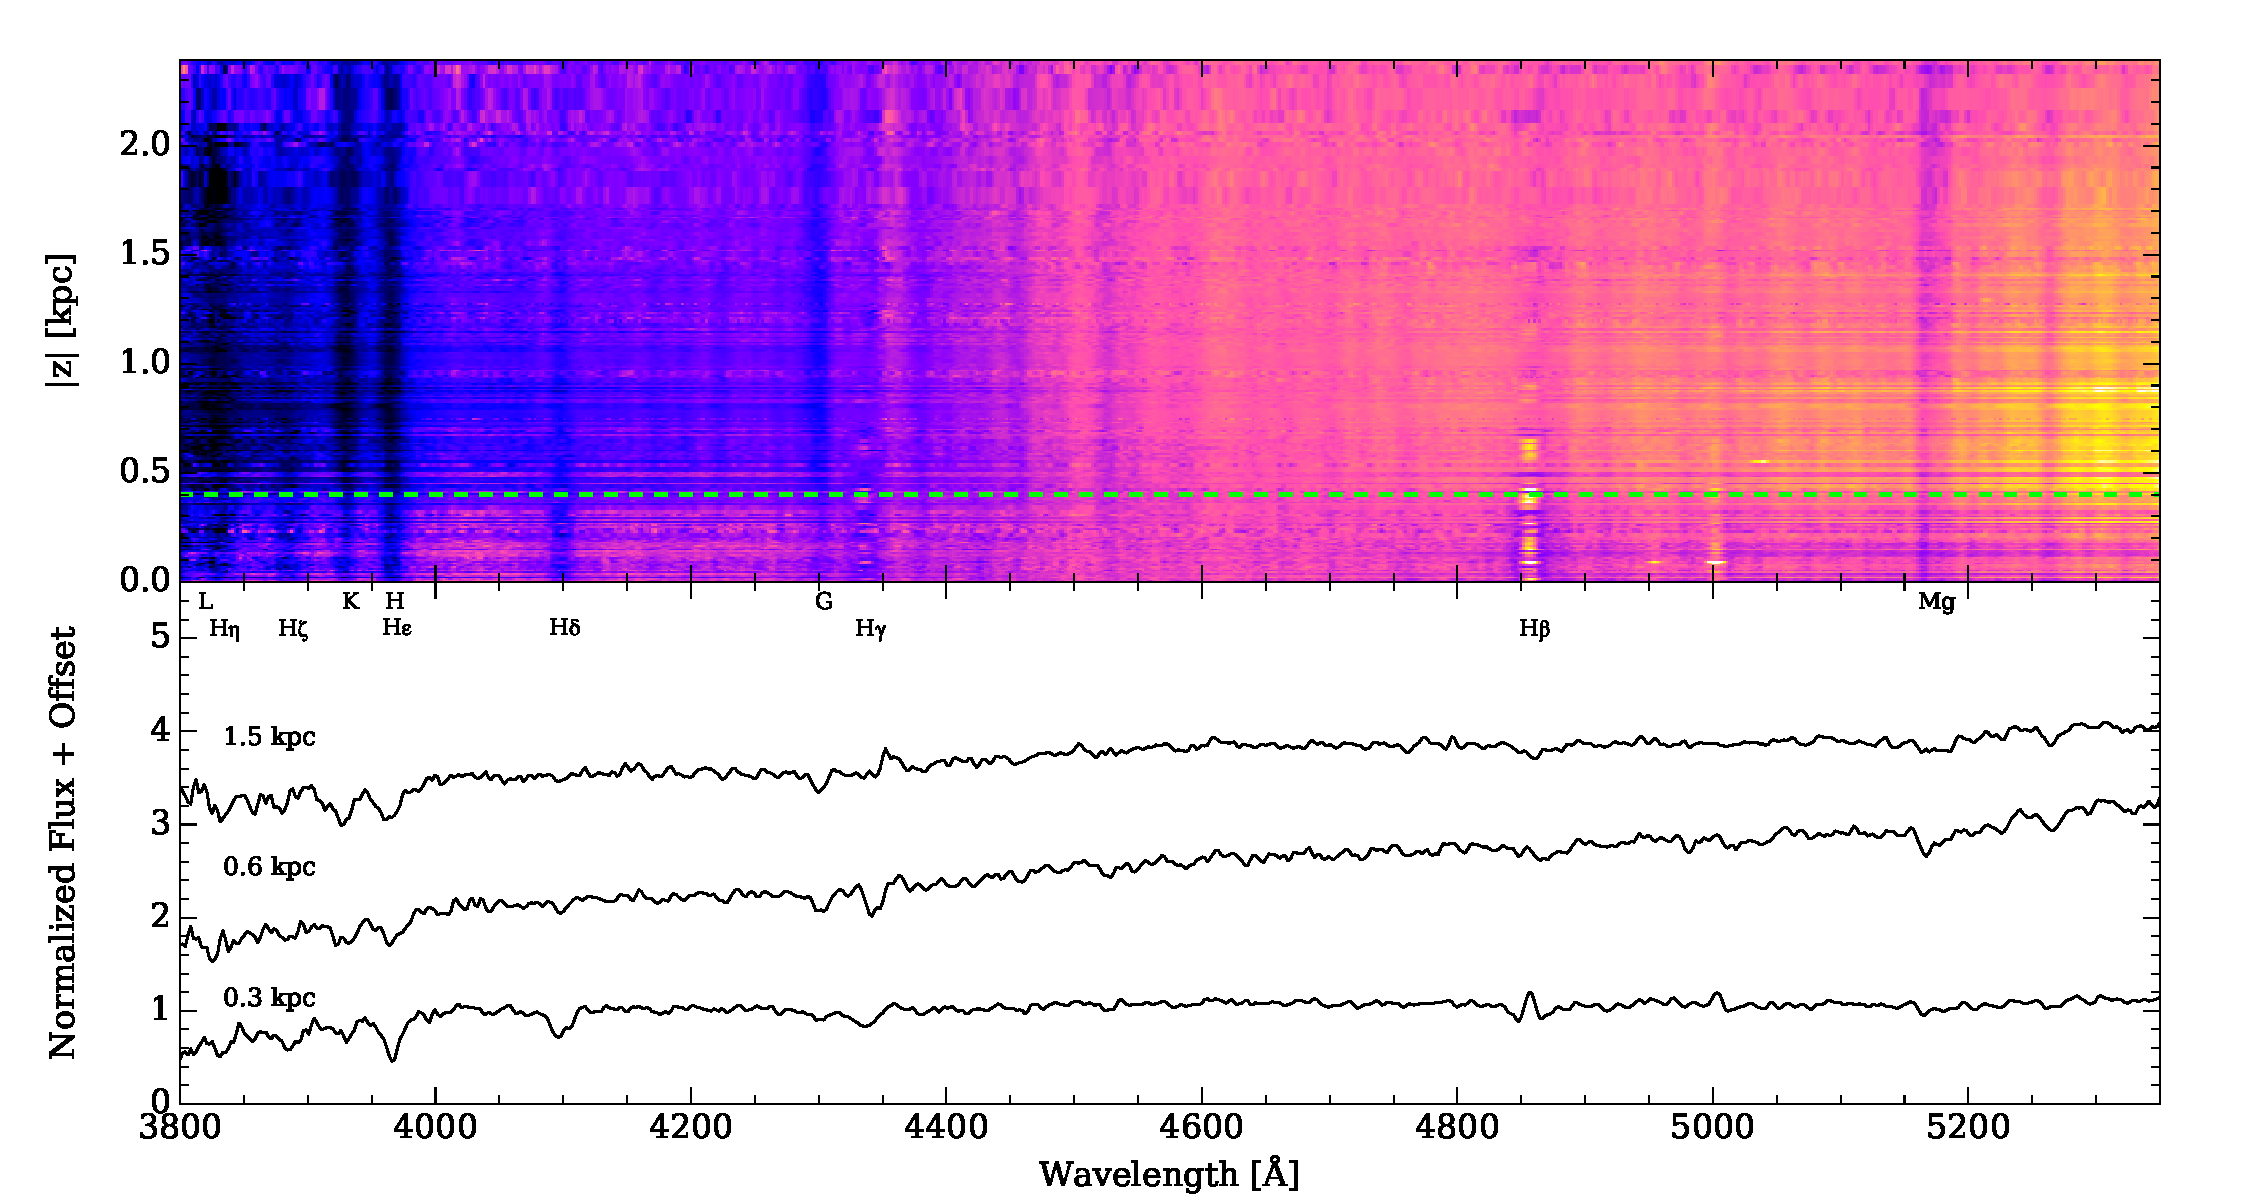
\includegraphics[width=\textwidth]{891_1/figs/mab_data_stack.pdf}
  \caption[Heating signature in NGC 891 \GP
  data]{\label{891_1:fig:mab_data}\fixspacing Same as Figure
    \ref{891_1:fig:MW_heating}, but for the \GP data from NGC 891. Top:
    Normalized galaxy spectra at different heights, color-coded by
    intensity (see text for a description of how this image was
    made). The horizontal line marks the age break at \val{0.4}{kpc}
    described for Figure \ref{891_1:fig:D4000_cuts}. Bottom: Representative
    spectra at three different heights (labeled). Prominent spectral
    features are labeled at the boundary between the two panels.}
\end{figure*}

\subsection{Vertical Trends}

The almost perfectly edge-on nature of NGC 891 allows unambiguous
determination of vertical trends in our spectra. Figure
\ref{891_1:fig:mab_data} presents our data for direct comparison to Figure
\ref{891_1:fig:MW_heating}. This was made by sorting spectra from all
apertures by height, regardless of radius, and then interpolating them
onto a regular grid to form a linear scale in kpc. The grid spacing (8
pc) was chosen for cosmetic reasons to keep the interpolation from
being apparent except at the largest heights. As with the model
spectra in Figure \ref{891_1:fig:MW_heating}, the individual spectra were
first normalized by their mean value.

% Apertures for spectra in \ref{fig:mab_data}
% 0.3 kpc - P6.12
% 0.6 kpc - P3.32
% 1.5 kpc - P6.33

The transition from young, Balmer-dominated spectra to
old, metal-dominated spectra is clear at \val{0.4}{kpc}, as
highlighted by the example spectra. At \val{0.3}{kpc} Balmer
absorption dominates, but a larger heights strong Ca H\&K and G band
absorption indicate the presence of older populations.  The amazing
match between Figures \ref{891_1:fig:MW_heating} and \ref{891_1:fig:mab_data} is
even more remarkable given that the MW heating model used in Figure
\ref{891_1:fig:MW_heating} includes no information about NGC 891 and is
simply tuned to observations from the Solar Cylinder.

This first-blush qualitative comparison has visceral appeal, and
demonstrates the vertical trends in stellar populations seen in the MW
(as described in \S\ref{891_1:sec:introduction}) are manifest in NGC
891. However, the comparison lacks quantitative rigor.  Our primary
interest is to quantify the comparison and determine to what extent
these trends also depend on radius. In particular, precise location of
a sharp vertical transition from Balmer-line to metal-line dominated
spectra can be used to calibrate how disk stars are vertically
stratified in phase space as a function of age and radial
location. This in turn can be interpreted in terms of time-scales for
dynamical heating or gas-cooling models, and the extent to which
vertical age gradients in spiral disks are ubiquitous and
quantitatively similar or distinct.

Disentangling age from metallicity, and metallicity from abundance is
fraught with degeneracies, particularly in complex stellar populations
observed in integrated star-light. In an edge-on galaxy like NGC 891,
there is the additional complication of projection effects compounded
with extinction that is patchy, but also changes broadly with height
and radius. Paper II undertakes to model all of these complexities,
but here we are interested in using simple spectral indices, the
measured value of which are model-independent and insensitive to
redenning. These indices allow us to we probe for vertical {\it age}
transitions and their radial trends while at the same time bounding
(providing priors on) the age and metallicity of the more complicated
modeling we later undertake.

\subsection{Spectral Indices}
\label{891_1:sec:indices}

\subsubsection{Definitions}
\label{891_1:sec:index_defn}

We focus our attention on the spectral indices defined in Table
\ref{891_1:tab:indices}. The first two entries have primary sensitivity to
age, while the remainder are primarily sensitive to metallicity, and,
in combination, to abundance. Because the age-sensitive indices have
varying degrees of dependence on metallicity and vice versa, index
combinations are required to disentangle these effects, as well
established in the literature, particularly for older stellar
populations, as we cite in what follows.

The strength of Balmer absorption has long been used as a mostly
metallicity-insensitive measure of population age because it depends
primarily on the main-sequence turn off temperature instead of the red
giant branch temperature. In other words, strong Balmer absorption is
produced by young, hot main-sequence stars with lifetimes of
$<\val{100}{Myr}$, regardless of metal content. \citet{Worthey97} find
that of the Balmer absorption lines \HB is the least sensitive to
metallicity (due to a lack of adjacent metal lines that impact the
continuum) and, given its relative strength, is the most sensitive to
age.  However, contamination from nebular emission is problematic,
with increasing intensity for the lower-order Balmer lines.  All of
our spectra show strong signs of \Ha emission and in some apertures
Balmer lines have negative equivalent widths as high as \Hg.  The
traditional trade between age sensitivity (i.e., \emph{insensitivity}
to metallicity variations) and systematics due to nebular emission, is
to use \Hda \citep{Worthey97} as an age indicator, which in fact has
long been used in extragalactic studies of mixed stellar populations
\citep[e.g.,][]{Couch87}. In Paper II we develop a model for Balmer
emission and find that applying an emission correction correction
shifts \Hda by \val{-0.4\pm 0.3}{\AA}, which is roughly 10\% of the
dynamic range in \Hda across the age transition found in
\S\ref{891_1:sec:age_grad}.

The break at \val{4000}{\AA} can also be used to estimate the age of
stellar populations, albeit with a larger sensitivity to
metallicity. This break is caused by an increase in opacity resulting
from ionization of metal lines; young stars are hot enough to put
metals into high ionization states and the thus the total opacity is
low. As temperature decreases more of the metals occupy lower
ionization states that are suitable for absorption and the opacity
increases. Beyond a certain limit very cool stars (i.e., M stars) are
unable to even singly ionize the neutral atoms and the amplitude of
the break decreases. Thus the \val{4000}{\AA} break traces population
age (specifically related to the temperature of the red giant branch),
but also depends on the population metallicity, although not as
strongly \citep[see][and Figure \ref{891_1:fig:D4000_cuts} here]{Bruzual83}.
The metal line that contributes most to the \val{4000}{\AA} break is
Ca K at \val{3933}{\AA}, which causes the magnitude of the break to
also exhibit a weak dependence on abundance. To measure the
\val{4000}{\AA} break we use the narrower-band definition of
\citet{Balogh99} primarily because our flux calibration deteriorates
blueward of \val{3800}{\AA} (Figure \ref{891_1:fig:sky_flux_comp}), and we
adopt the nomenclature, $D_n(4000)$, of \citet{Kauffmann03}.

We also define composite indices to determine metallicity and
$\alpha$-enhancement in our populations. In particular,
\citet{Thomas03} find that 
\begin{equation}
\mathrm{[MgFe]} = \sqrt{\mathrm{Mg
    \emph{b}}(0.72\times\mathrm{Fe}_{5270} +
  0.28\times\mathrm{Fe}_{5335})}
\end{equation}
is almost totally insensitive to changes in abundance and is therefore
a good tracer of the total metallicity in a stellar population. They
also note that, when plotted against Mg$b$, Fe$_{5270}$, Fe$_{5335}$,
and Fe$_{5408}$ are all fairly sensitive to changes in abundance. We
choose to use $\left<\mathrm{Fe}\right>$ =
(Fe$_{5270}$+Fe$_{5335}$)/2, because these two Fe indices are slightly
better calibrated than Fe$_{5408}$ \citep{Thomas03} and have been have
been used in other important studies
\citep[e.g.,][]{Trager05,Trager08,Trager09}.

The reported ``indices'' are equivalent widths defined as
\begin{equation}
  EW = \left(1 - \frac{F_I}{F_C}\right)\Delta_{\lambda},
\end{equation}
where $F_I$ and $F_C$ are the average fluxes in the index and
continuum bands, respectively and $\Delta_{\lambda}$ is the width of
the index bandpass defined in Table \ref{891_1:tab:indices}. The value of
$F_C$ is computed by linearly interpolating the flux computed in the
red and blue continuum bands to the center of the index band. In the
case of $D_n(4000)$ the reported value is simply the ratio of the
average flux in the red continuum band to the average flux in the blue
continuum band. Table \ref{tab:index_res_full} reports our measured values
for all appertures defined in Table \ref{tab:data_ap_full}.

Recognizing the wisdom of \citet{Balogh99} we caution that the
absolute values of our measured indices do not correspond to physical
quantities. The specific conditions of our data (e.g., spectral
resolution, sampling, signal-to-noise, etc.) can and will affect the
derived index values and the reader is warned away from comparing our
results in an absolute sense to those of other studies unless they are
careful to match to our spectral sampling and resolution as described
in Section \ref{891_1:sec:obs}.

\begin{deluxetable}{lccccccc}
\tablewidth{0pt}
\tablecaption{Spectral Index Definitions}
\tablehead{
%  & \multicolumn{6}{c}{Bandpass (\AA)}\\
%  & \multicolumn{6}{\hline}\\
  \colhead{Index} &
  \multicolumn{2}{c}{On-Band} &
  \multicolumn{2}{c}{Blue Continuum} &
  \multicolumn{2}{c}{Red Continuum} \\
  \colhead{Name} &
  \colhead{Center} &
  \colhead{Width} &
  \colhead{Center} &
  \colhead{Width} &
  \colhead{Center} &
  \colhead{Width}\\
  \colhead{} &
  \colhead{(\AA)} &
  \colhead{(\AA)} &
  \colhead{(\AA)} &
  \colhead{(\AA)} &
  \colhead{(\AA)} &
  \colhead{(\AA)}}
\startdata
$D_n(4000)$ & - & - & 3900 & 100 & 4050 & 100 \\
H$\delta_A$ & 4103.9 & 38.8 & 4060.7 & 38.1 & 4144.8 & 32.5 \\
%H$\gamma_A$ & 4341.6 & 43.8 & 4301.6 & 36.3 & 4393.5 & 52.5 \\
%\HB         & 4862.3 & 28.8 & 4837.9 & 20.0 & 4884.1 & 15.0 \\
Mg\emph{b} & 5176.4 & 32.5 & 5152.0 & 18.8 & 5198.9 & 15.0 \\
Fe$_{5270}$  & 5265.7 & 40.0 & 5240.7 & 15.0 & 5301.9 & 32.5 \\
Fe$_{5335}$  & 5332.1 & 40.0 & 5310.3 & 11.3 & 5358.4 & 10.0
\enddata
\label{891_1:tab:indices}
\end{deluxetable}

\clearpage
\begin{deluxetable}{ccccccccc}
\tablewidth{0pt}
\tablecaption{NGC 891 Index Measurements}
\tablehead{
    \colhead{Pointing} &
    \colhead{Aperture} &
    \colhead{$r_\mathrm{proj}$} &
    \colhead{$z$} &
    \colhead{$D_n4000$} &
    \colhead{$H\delta_A$} &
    \colhead{Mg$b$} &
    \colhead{$\left<\mathrm{Fe}\right>$} &
    \colhead{[MgFe]}\\
    \colhead{Number} &
    \colhead{Number} &
    \colhead{(kpc)} &
    \colhead{(kpc)} &
    \colhead{} &
    \colhead{(\AA)} &
    \colhead{(\AA)} &
    \colhead{(\AA)} &
    \colhead{(\AA)}
}
\startdata
 1 &  1 & 4.44 & -0.12 & 1.64 $\pm$ 0.04 & 5.91 $\pm$ 0.85 & 1.99 $\pm$ 0.47 & 0.76 $\pm$ 0.37 & 1.36 $\pm$ 0.32\\
 1 &  2 & 5.26 & -0.09 & 1.20 $\pm$ 0.02 & 4.20 $\pm$ 0.78 & 1.43 $\pm$ 0.56 & 0.95 $\pm$ 0.46 & 1.35 $\pm$ 0.35\\
  %%  1 &  3 & 4.16 & 0.02 & 1.37 $\pm$ 0.03 & 2.63 $\pm$ 1.01 & 2.27 $\pm$ 0.56 & 1.54 $\pm$ 0.40 & 1.91 $\pm$ 0.34\\
  %%  1 &  4 & 4.76 & 0.04 & 1.29 $\pm$ 0.02 & 4.64 $\pm$ 0.62 & 2.09 $\pm$ 0.49 & 1.07 $\pm$ 0.40 & 1.51 $\pm$ 0.33\\
  %%  1 &  5 & 5.52 & 0.07 & 1.11 $\pm$ 0.05 & 7.10 $\pm$ 1.77 & 2.49 $\pm$ 0.95 & -0.16 $\pm$ 0.92 &  nan $\pm$  nan\\
  %%  1 &  6 & 4.67 & 0.21 & 1.29 $\pm$ 0.02 & 5.19 $\pm$ 0.71 & 1.73 $\pm$ 0.52 & 0.81 $\pm$ 0.41 & 1.03 $\pm$ 0.39\\
  %%  1 &  7 & 5.51 & 0.24 & 1.32 $\pm$ 0.05 & 5.38 $\pm$ 1.59 & 1.66 $\pm$ 0.94 & 0.67 $\pm$ 0.91 & 0.86 $\pm$ 0.85\\
  %%  1 &  8 & 4.47 & 0.41 & 1.17 $\pm$ 0.02 & 6.28 $\pm$ 0.64 & 1.52 $\pm$ 0.49 & 1.46 $\pm$ 0.39 & 1.65 $\pm$ 0.32\\
  %%  1 &  9 & 5.24 & 0.44 & 1.51 $\pm$ 0.03 & 1.90 $\pm$ 0.85 & 1.89 $\pm$ 0.39 & 1.40 $\pm$ 0.28 & 1.77 $\pm$ 0.23\\
  %%  1 & 10 & 5.68 & 0.46 & 1.63 $\pm$ 0.05 & 2.02 $\pm$ 1.25 & 1.89 $\pm$ 0.54 & 1.60 $\pm$ 0.45 & 1.95 $\pm$ 0.36\\
  %%  1 & 11 & 4.61 & 0.63 & 1.61 $\pm$ 0.03 & 2.30 $\pm$ 0.71 & 1.86 $\pm$ 0.35 & 1.52 $\pm$ 0.30 & 1.79 $\pm$ 0.22\\
  %%  1 & 12 & 5.45 & 0.67 & 1.84 $\pm$ 0.04 & 2.08 $\pm$ 0.84 & 1.85 $\pm$ 0.48 & 1.46 $\pm$ 0.33 & 1.76 $\pm$ 0.29\\
  %%  1 & 13 & 5.67 & 0.68 & 1.84 $\pm$ 0.05 & 2.40 $\pm$ 0.83 & 2.11 $\pm$ 0.40 & 1.62 $\pm$ 0.36 & 1.90 $\pm$ 0.26\\
  %%  1 & 14 & 4.22 & 0.87 & 1.71 $\pm$ 0.04 & 1.50 $\pm$ 0.78 & 1.85 $\pm$ 0.36 & 1.37 $\pm$ 0.37 & 1.65 $\pm$ 0.25\\
  %%  1 & 15 & 4.62 & 0.89 & 1.72 $\pm$ 0.04 & 0.81 $\pm$ 0.90 & 2.20 $\pm$ 0.46 & 1.50 $\pm$ 0.45 & 1.95 $\pm$ 0.30\\
  %%  1 & 16 & 4.89 & 0.90 & 1.75 $\pm$ 0.04 & 1.56 $\pm$ 0.96 & 2.46 $\pm$ 0.55 & 1.33 $\pm$ 0.54 & 1.95 $\pm$ 0.38\\
  %%  1 & 17 & 5.16 & 0.91 & 1.74 $\pm$ 0.04 & 1.61 $\pm$ 0.83 & 2.48 $\pm$ 0.52 & 1.52 $\pm$ 0.50 & 2.06 $\pm$ 0.34\\
  %%  1 & 18 & 5.43 & 0.92 & 1.58 $\pm$ 0.04 & 1.19 $\pm$ 0.75 & 1.90 $\pm$ 0.47 & 1.31 $\pm$ 0.42 & 1.66 $\pm$ 0.29\\
  %%  1 & 19 & 5.69 & 0.94 & 1.75 $\pm$ 0.04 & 0.08 $\pm$ 0.90 & 1.92 $\pm$ 0.51 & 1.79 $\pm$ 0.50 & 1.96 $\pm$ 0.33\\
  %%  1 & 20 & 4.07 & 1.14 & 1.62 $\pm$ 0.04 & 1.59 $\pm$ 0.94 & 2.48 $\pm$ 0.55 & 1.13 $\pm$ 0.54 & 1.79 $\pm$ 0.39\\
  %%  1 & 21 & 4.34 & 1.15 & 1.63 $\pm$ 0.03 & 0.92 $\pm$ 0.82 & 2.23 $\pm$ 0.36 & 1.63 $\pm$ 0.34 & 2.06 $\pm$ 0.24\\
  %%  1 & 22 & 4.61 & 1.16 & 1.65 $\pm$ 0.04 & 2.07 $\pm$ 0.98 & 2.33 $\pm$ 0.45 & 1.37 $\pm$ 0.47 & 1.89 $\pm$ 0.30\\
  %%  1 & 23 & 4.88 & 1.17 & 1.57 $\pm$ 0.03 & 0.86 $\pm$ 0.71 & 2.25 $\pm$ 0.33 & 1.45 $\pm$ 0.38 & 1.87 $\pm$ 0.26\\
  %%  1 & 24 & 5.15 & 1.18 & 1.60 $\pm$ 0.03 & 1.33 $\pm$ 0.72 & 2.41 $\pm$ 0.52 & 2.00 $\pm$ 0.48 & 2.31 $\pm$ 0.34\\
  %%  1 & 25 & 5.55 & 1.20 & 1.56 $\pm$ 0.03 & 0.10 $\pm$ 0.85 & 2.15 $\pm$ 0.47 & 1.29 $\pm$ 0.48 & 1.84 $\pm$ 0.32\\
  %%  1 & 26 & 4.06 & 1.40 & 1.63 $\pm$ 0.03 & 0.53 $\pm$ 0.67 & 1.93 $\pm$ 0.41 & 1.53 $\pm$ 0.36 & 1.77 $\pm$ 0.26\\
  %%  1 & 27 & 4.33 & 1.42 & 1.54 $\pm$ 0.03 & 0.54 $\pm$ 0.72 & 2.20 $\pm$ 0.39 & 1.43 $\pm$ 0.38 & 1.86 $\pm$ 0.26\\
  %%  1 & 28 & 4.60 & 1.43 & 1.55 $\pm$ 0.03 & 0.67 $\pm$ 0.71 & 2.22 $\pm$ 0.49 & 1.64 $\pm$ 0.48 & 2.00 $\pm$ 0.32\\
  %%  1 & 29 & 5.00 & 1.44 & 1.50 $\pm$ 0.03 & 0.69 $\pm$ 0.75 & 2.09 $\pm$ 0.48 & 1.58 $\pm$ 0.48 & 1.91 $\pm$ 0.32\\
  %%  1 & 30 & 5.54 & 1.47 & 1.42 $\pm$ 0.04 & -1.41 $\pm$ 1.21 & 1.72 $\pm$ 0.73 & 0.53 $\pm$ 0.79 & 1.10 $\pm$ 0.58\\
  %%  1 & 31 & 4.04 & 1.71 & 1.54 $\pm$ 0.03 & 0.18 $\pm$ 0.79 & 2.93 $\pm$ 0.39 & 1.20 $\pm$ 0.33 & 1.96 $\pm$ 0.27\\
  %%  1 & 32 & 4.37 & 1.72 & 1.52 $\pm$ 0.03 & 0.49 $\pm$ 0.82 & 2.24 $\pm$ 0.44 & 1.36 $\pm$ 0.37 & 1.88 $\pm$ 0.28\\
  %%  1 & 33 & 4.85 & 1.75 & 1.65 $\pm$ 0.03 & 1.01 $\pm$ 0.76 & 2.42 $\pm$ 0.48 & 1.27 $\pm$ 0.33 & 1.79 $\pm$ 0.28\\
  %%  1 & 34 & 5.50 & 1.77 & 1.87 $\pm$ 0.05 & -0.46 $\pm$ 0.99 & 1.71 $\pm$ 0.62 & 1.85 $\pm$ 0.48 & 1.82 $\pm$ 0.40\\
  %%  1 & 35 & 4.19 & 2.04 & 1.54 $\pm$ 0.03 & -0.83 $\pm$ 0.90 & 2.95 $\pm$ 0.40 & 1.20 $\pm$ 0.32 & 2.09 $\pm$ 0.27\\
  %%  1 & 36 & 5.16 & 2.08 & 1.55 $\pm$ 0.03 & 0.82 $\pm$ 0.90 & 2.47 $\pm$ 0.50 & 1.26 $\pm$ 0.39 & 1.92 $\pm$ 0.32\\
  %%  1 & 37 & 4.82 & 2.39 & 1.28 $\pm$ 0.02 & -0.50 $\pm$ 0.93 & 1.76 $\pm$ 0.48 & 1.24 $\pm$ 0.42 & 1.56 $\pm$ 0.31\\
 2 &  1 & 1.27 & -0.17 & 1.41 $\pm$ 0.08 & -0.71 $\pm$ 2.54 & 2.95 $\pm$ 1.02 & 1.68 $\pm$ 0.78 & 2.22 $\pm$ 0.64\\
 2 &  2 & 1.26 & -0.02 & 1.10 $\pm$ 0.04 & 7.57 $\pm$ 1.44 & 1.47 $\pm$ 1.06 & 0.65 $\pm$ 0.68 & 1.06 $\pm$ 0.63\\
  %%  2 &  3 & 1.26 & 0.15 & 1.25 $\pm$ 0.04 & 6.53 $\pm$ 1.07 & 0.83 $\pm$ 0.75 & -0.01 $\pm$ 0.69 &  nan $\pm$  nan\\
  %%  2 &  4 & 1.25 & 0.35 & 1.45 $\pm$ 0.02 & 2.99 $\pm$ 0.64 & 1.91 $\pm$ 0.36 & 1.65 $\pm$ 0.38 & 1.86 $\pm$ 0.25\\
  %%  2 &  5 & 0.69 & 0.55 & 1.68 $\pm$ 0.03 & 0.39 $\pm$ 0.72 & 1.95 $\pm$ 0.44 & 1.53 $\pm$ 0.39 & 1.84 $\pm$ 0.29\\
  %%  2 &  6 & 1.35 & 0.58 & 1.81 $\pm$ 0.04 & 1.59 $\pm$ 0.64 & 2.22 $\pm$ 0.33 & 1.71 $\pm$ 0.29 & 2.09 $\pm$ 0.21\\
  %%  2 &  7 & 1.90 & 0.60 & 1.83 $\pm$ 0.05 & 1.05 $\pm$ 1.10 & 2.19 $\pm$ 0.49 & 1.39 $\pm$ 0.39 & 1.86 $\pm$ 0.31\\
  %%  2 &  8 & 0.42 & 0.79 & 1.88 $\pm$ 0.03 & 0.21 $\pm$ 0.61 & 2.26 $\pm$ 0.19 & 1.56 $\pm$ 0.15 & 1.94 $\pm$ 0.12\\
  %%  2 &  9 & 0.69 & 0.81 & 1.76 $\pm$ 0.03 & 1.16 $\pm$ 0.51 & 1.21 $\pm$ 0.24 & 0.67 $\pm$ 0.19 & 1.08 $\pm$ 0.14\\
  %%  2 & 10 & 0.96 & 0.82 & 1.81 $\pm$ 0.02 & 0.66 $\pm$ 0.45 & 2.09 $\pm$ 0.24 & 1.24 $\pm$ 0.21 & 1.73 $\pm$ 0.16\\
  %%  2 & 11 & 1.23 & 0.83 & 1.84 $\pm$ 0.03 & 1.09 $\pm$ 0.69 & 2.12 $\pm$ 0.35 & 1.24 $\pm$ 0.25 & 1.72 $\pm$ 0.21\\
  %%  2 & 12 & 1.49 & 0.84 & 1.75 $\pm$ 0.03 & 0.42 $\pm$ 0.65 & 1.88 $\pm$ 0.24 & 1.50 $\pm$ 0.24 & 1.81 $\pm$ 0.16\\
  %%  2 & 13 & 1.76 & 0.85 & 1.67 $\pm$ 0.04 & 0.14 $\pm$ 0.82 & 2.45 $\pm$ 0.24 & 1.54 $\pm$ 0.22 & 1.97 $\pm$ 0.17\\
  %%  2 & 14 & 2.03 & 0.86 & 1.67 $\pm$ 0.04 & 1.51 $\pm$ 1.01 & 1.74 $\pm$ 0.38 & 1.09 $\pm$ 0.27 & 1.56 $\pm$ 0.22\\
  %%  2 & 15 & 0.41 & 1.06 & 1.76 $\pm$ 0.03 & 0.35 $\pm$ 0.60 & 2.04 $\pm$ 0.27 & 1.59 $\pm$ 0.24 & 1.88 $\pm$ 0.18\\
  %%  2 & 16 & 0.68 & 1.07 & 1.72 $\pm$ 0.03 & 0.72 $\pm$ 0.57 & 1.59 $\pm$ 0.37 & 1.06 $\pm$ 0.24 & 1.38 $\pm$ 0.20\\
  %%  2 & 17 & 0.95 & 1.08 & 1.68 $\pm$ 0.02 & -0.21 $\pm$ 0.56 & 2.18 $\pm$ 0.29 & 1.21 $\pm$ 0.29 & 1.76 $\pm$ 0.20\\
  %%  2 & 18 & 1.21 & 1.10 & 1.71 $\pm$ 0.03 & 0.89 $\pm$ 0.53 & 2.06 $\pm$ 0.29 & 1.15 $\pm$ 0.23 & 1.64 $\pm$ 0.17\\
  %%  2 & 19 & 1.48 & 1.11 & 1.69 $\pm$ 0.03 & 1.31 $\pm$ 0.68 & 2.04 $\pm$ 0.33 & 1.29 $\pm$ 0.24 & 1.76 $\pm$ 0.19\\
  %%  2 & 20 & 1.75 & 1.12 & 1.68 $\pm$ 0.03 & -0.04 $\pm$ 0.80 & 2.61 $\pm$ 0.35 & 1.58 $\pm$ 0.32 & 2.14 $\pm$ 0.23\\
  %%  2 & 21 & 2.02 & 1.13 & 1.53 $\pm$ 0.04 & 1.09 $\pm$ 0.78 & 1.76 $\pm$ 0.42 & 0.37 $\pm$ 0.38 & 1.00 $\pm$ 0.35\\
  %%  2 & 22 & 0.40 & 1.33 & 1.69 $\pm$ 0.03 & -0.22 $\pm$ 0.81 & 1.87 $\pm$ 0.36 & 1.35 $\pm$ 0.39 & 1.67 $\pm$ 0.28\\
  %%  2 & 23 & 0.67 & 1.34 & 1.68 $\pm$ 0.03 & 0.58 $\pm$ 0.65 & 2.07 $\pm$ 0.37 & 1.07 $\pm$ 0.27 & 1.51 $\pm$ 0.25\\
  %%  2 & 24 & 0.93 & 1.35 & 1.65 $\pm$ 0.02 & 0.05 $\pm$ 0.73 & 1.85 $\pm$ 0.34 & 1.49 $\pm$ 0.35 & 1.73 $\pm$ 0.23\\
  %%  2 & 25 & 1.20 & 1.36 & 1.60 $\pm$ 0.03 & -0.26 $\pm$ 0.65 & 2.24 $\pm$ 0.48 & 1.57 $\pm$ 0.44 & 1.95 $\pm$ 0.34\\
  %%  2 & 26 & 1.47 & 1.38 & 1.65 $\pm$ 0.03 & 0.14 $\pm$ 0.69 & 2.28 $\pm$ 0.46 & 1.50 $\pm$ 0.38 & 1.86 $\pm$ 0.30\\
  %%  2 & 27 & 1.74 & 1.39 & 1.60 $\pm$ 0.04 & 0.61 $\pm$ 0.91 & 2.19 $\pm$ 0.44 & 1.30 $\pm$ 0.45 & 1.81 $\pm$ 0.31\\
  %%  2 & 28 & 2.01 & 1.40 & 1.56 $\pm$ 0.05 & 0.70 $\pm$ 0.96 & 1.85 $\pm$ 0.78 & 1.51 $\pm$ 0.56 & 1.65 $\pm$ 0.50\\
  %%  2 & 29 & 0.38 & 1.64 & 1.58 $\pm$ 0.04 & -0.92 $\pm$ 0.97 & 1.96 $\pm$ 0.41 & 1.28 $\pm$ 0.43 & 1.75 $\pm$ 0.28\\
  %%  2 & 30 & 0.70 & 1.65 & 1.55 $\pm$ 0.03 & -0.55 $\pm$ 0.79 & 1.88 $\pm$ 0.54 & 0.91 $\pm$ 0.38 & 1.38 $\pm$ 0.31\\
  %%  2 & 31 & 1.03 & 1.67 & 1.69 $\pm$ 0.04 & 0.42 $\pm$ 0.84 & 1.64 $\pm$ 0.63 & 0.49 $\pm$ 0.53 & 1.09 $\pm$ 0.41\\
  %%  2 & 32 & 1.35 & 1.68 & 1.60 $\pm$ 0.04 & 0.81 $\pm$ 0.90 & 1.81 $\pm$ 0.48 & 0.87 $\pm$ 0.34 & 1.39 $\pm$ 0.32\\
  %%  2 & 33 & 1.68 & 1.69 & 1.66 $\pm$ 0.04 & 2.20 $\pm$ 1.04 & 1.88 $\pm$ 0.58 & 1.16 $\pm$ 0.43 & 1.64 $\pm$ 0.36\\
  %%  2 & 34 & 2.00 & 1.71 & 1.63 $\pm$ 0.04 & 0.73 $\pm$ 0.89 & 1.45 $\pm$ 0.54 & 0.56 $\pm$ 0.47 & 0.98 $\pm$ 0.40\\
  %%  2 & 35 & 0.36 & 1.96 & 1.51 $\pm$ 0.04 & -0.46 $\pm$ 1.03 & -0.20 $\pm$ 0.51 & -0.34 $\pm$ 0.41 & 0.26 $\pm$ 0.36\\
  %%  2 & 36 & 1.18 & 2.00 & 1.53 $\pm$ 0.03 & 0.45 $\pm$ 0.78 & 1.80 $\pm$ 0.43 & 0.88 $\pm$ 0.35 & 1.32 $\pm$ 0.28\\
  %%  2 & 37 & 1.99 & 2.03 & 1.44 $\pm$ 0.06 & 0.37 $\pm$ 1.58 & 0.55 $\pm$ 1.16 & 1.30 $\pm$ 0.72 & 0.94 $\pm$ 1.02\\
  %%  2 & 38 & 1.16 & 2.32 & 1.35 $\pm$ 0.03 & 0.25 $\pm$ 0.95 & 1.60 $\pm$ 0.57 & 0.80 $\pm$ 0.48 & 1.22 $\pm$ 0.37\\
 3 &  1 & -6.31 & -0.17 & 1.52 $\pm$ 0.02 & 4.36 $\pm$ 0.50 & 1.42 $\pm$ 0.38 & 1.30 $\pm$ 0.30 & 1.43 $\pm$ 0.24\\
 3 &  2 & -5.98 & -0.16 & 1.29 $\pm$ 0.02 & 4.49 $\pm$ 0.70 & 1.34 $\pm$ 0.49 & 1.14 $\pm$ 0.36 & 1.36 $\pm$ 0.30\\
  %%  3 &  3 & -5.76 & -0.15 & 1.30 $\pm$ 0.02 & 3.37 $\pm$ 0.72 & 1.89 $\pm$ 0.52 & 0.78 $\pm$ 0.45 & 1.31 $\pm$ 0.34\\
  %%  3 &  4 & -5.43 & -0.14 & 1.18 $\pm$ 0.01 & 3.06 $\pm$ 0.57 & 2.07 $\pm$ 0.51 & 1.22 $\pm$ 0.42 & 1.70 $\pm$ 0.32\\
  %%  3 &  5 & -5.05 & -0.12 & 1.18 $\pm$ 0.01 & 5.42 $\pm$ 0.56 & 1.76 $\pm$ 0.49 & 1.33 $\pm$ 0.37 & 1.53 $\pm$ 0.29\\
  %%  3 &  6 & -6.39 & -0.03 & 1.16 $\pm$ 0.01 & 5.14 $\pm$ 0.40 & 1.30 $\pm$ 0.39 & 0.93 $\pm$ 0.35 & 1.13 $\pm$ 0.26\\
  %%  3 &  7 & -6.13 & -0.01 & 1.16 $\pm$ 0.01 & 4.03 $\pm$ 0.47 & 0.88 $\pm$ 0.46 & 0.57 $\pm$ 0.36 & 0.80 $\pm$ 0.28\\
  %%  3 &  8 & -5.97 & -0.01 & 1.13 $\pm$ 0.01 & 3.85 $\pm$ 0.49 & 0.58 $\pm$ 0.35 & 0.33 $\pm$ 0.31 & 0.55 $\pm$ 0.23\\
  %%  3 &  9 & -5.80 & 0.00 & 1.09 $\pm$ 0.01 & 4.46 $\pm$ 0.50 & 1.36 $\pm$ 0.46 & 0.81 $\pm$ 0.40 & 1.14 $\pm$ 0.30\\
  %%  3 & 10 & -5.63 & 0.01 & 1.19 $\pm$ 0.02 & 3.11 $\pm$ 0.81 & 1.30 $\pm$ 0.46 & 0.84 $\pm$ 0.43 & 1.09 $\pm$ 0.32\\
  %%  3 & 11 & -5.46 & 0.01 & 1.21 $\pm$ 0.01 & 4.54 $\pm$ 0.46 & 1.75 $\pm$ 0.35 & 0.92 $\pm$ 0.32 & 1.35 $\pm$ 0.24\\
  %%  3 & 12 & -5.20 & 0.03 & 1.19 $\pm$ 0.01 & 4.70 $\pm$ 0.46 & 1.79 $\pm$ 0.34 & 0.54 $\pm$ 0.27 & 1.09 $\pm$ 0.24\\
  %%  3 & 13 & -4.95 & 0.04 & 1.20 $\pm$ 0.01 & 3.63 $\pm$ 0.63 & 1.28 $\pm$ 0.57 & 0.56 $\pm$ 0.43 & 0.91 $\pm$ 0.37\\
  %%  3 & 14 & -6.48 & 0.14 & 1.26 $\pm$ 0.01 & 5.66 $\pm$ 0.41 & 0.94 $\pm$ 0.43 & 0.95 $\pm$ 0.38 & 1.07 $\pm$ 0.29\\
  %%  3 & 15 & -6.31 & 0.15 & 1.17 $\pm$ 0.01 & 5.07 $\pm$ 0.42 & 1.18 $\pm$ 0.33 & 0.86 $\pm$ 0.27 & 1.14 $\pm$ 0.21\\
  %%  3 & 16 & -6.14 & 0.15 & 1.21 $\pm$ 0.01 & 4.88 $\pm$ 0.50 & 0.99 $\pm$ 0.36 & 0.74 $\pm$ 0.31 & 0.82 $\pm$ 0.24\\
  %%  3 & 17 & -5.89 & 0.17 & 1.15 $\pm$ 0.01 & 4.11 $\pm$ 0.51 & 1.04 $\pm$ 0.40 & 0.68 $\pm$ 0.33 & 0.92 $\pm$ 0.25\\
  %%  3 & 18 & -5.55 & 0.18 & 1.21 $\pm$ 0.01 & 4.16 $\pm$ 0.55 & 1.17 $\pm$ 0.36 & 0.66 $\pm$ 0.28 & 0.99 $\pm$ 0.22\\
  %%  3 & 19 & -5.29 & 0.19 & 1.26 $\pm$ 0.02 & 1.92 $\pm$ 0.84 & 0.90 $\pm$ 0.54 & 0.96 $\pm$ 0.36 & 1.02 $\pm$ 0.35\\
  %%  3 & 20 & -5.04 & 0.20 & 1.30 $\pm$ 0.02 & 3.18 $\pm$ 0.58 & 1.28 $\pm$ 0.33 & 1.10 $\pm$ 0.28 & 1.27 $\pm$ 0.21\\
  %%  3 & 21 & -6.50 & 0.35 & 1.28 $\pm$ 0.02 & 4.71 $\pm$ 0.71 & 1.61 $\pm$ 0.35 & 1.09 $\pm$ 0.31 & 1.35 $\pm$ 0.23\\
  %%  3 & 22 & -6.28 & 0.36 & 1.25 $\pm$ 0.02 & 1.06 $\pm$ 0.93 & 1.33 $\pm$ 0.57 & 1.04 $\pm$ 0.44 & 1.24 $\pm$ 0.35\\
  %%  3 & 23 & -6.06 & 0.37 & 1.22 $\pm$ 0.01 & 2.99 $\pm$ 0.57 & 1.96 $\pm$ 0.36 & 1.10 $\pm$ 0.29 & 1.55 $\pm$ 0.23\\
  %%  3 & 24 & -5.84 & 0.38 & 1.20 $\pm$ 0.01 & 2.99 $\pm$ 0.55 & 1.71 $\pm$ 0.29 & 1.05 $\pm$ 0.26 & 1.43 $\pm$ 0.19\\
  %%  3 & 25 & -5.51 & 0.39 & 1.24 $\pm$ 0.01 & 2.28 $\pm$ 0.44 & 1.61 $\pm$ 0.33 & 1.09 $\pm$ 0.24 & 1.27 $\pm$ 0.20\\
  %%  3 & 26 & -5.18 & 0.40 & 1.37 $\pm$ 0.02 & 2.30 $\pm$ 0.55 & 2.04 $\pm$ 0.38 & 1.06 $\pm$ 0.32 & 1.55 $\pm$ 0.26\\
  %%  3 & 27 & -4.96 & 0.41 & 1.42 $\pm$ 0.02 & 0.05 $\pm$ 0.79 & 1.76 $\pm$ 0.41 & 1.15 $\pm$ 0.36 & 1.43 $\pm$ 0.28\\
  %%  3 & 28 & -6.51 & 0.57 & 1.55 $\pm$ 0.02 & 2.40 $\pm$ 0.57 & 2.13 $\pm$ 0.38 & 1.26 $\pm$ 0.36 & 1.74 $\pm$ 0.26\\
  %%  3 & 29 & -6.29 & 0.58 & 1.47 $\pm$ 0.02 & 4.63 $\pm$ 0.64 & 1.94 $\pm$ 0.35 & 1.63 $\pm$ 0.33 & 1.86 $\pm$ 0.23\\
  %%  3 & 30 & -6.07 & 0.59 & 1.48 $\pm$ 0.02 & 1.23 $\pm$ 0.70 & 2.33 $\pm$ 0.49 & 1.26 $\pm$ 0.43 & 1.77 $\pm$ 0.32\\
  %%  3 & 31 & -5.85 & 0.60 & 1.53 $\pm$ 0.02 & 0.90 $\pm$ 0.66 & 1.70 $\pm$ 0.40 & 1.48 $\pm$ 0.32 & 1.70 $\pm$ 0.25\\
  %%  3 & 32 & -5.41 & 0.61 & 1.60 $\pm$ 0.03 & 0.46 $\pm$ 0.68 & 2.05 $\pm$ 0.38 & 1.10 $\pm$ 0.30 & 1.56 $\pm$ 0.24\\
  %%  3 & 33 & -5.19 & 0.62 & 1.69 $\pm$ 0.03 & 1.54 $\pm$ 0.62 & 1.85 $\pm$ 0.27 & 1.39 $\pm$ 0.23 & 1.73 $\pm$ 0.17\\
  %%  3 & 34 & -4.97 & 0.63 & 1.55 $\pm$ 0.02 & 1.14 $\pm$ 0.68 & 1.81 $\pm$ 0.40 & 1.29 $\pm$ 0.30 & 1.58 $\pm$ 0.24\\
  %%  3 & 35 & -6.55 & 0.82 & 1.68 $\pm$ 0.02 & 0.06 $\pm$ 0.40 & 1.75 $\pm$ 0.25 & 1.31 $\pm$ 0.19 & 1.52 $\pm$ 0.15\\
  %%  3 & 36 & -6.29 & 0.83 & 1.47 $\pm$ 0.01 & 0.69 $\pm$ 0.43 & 1.90 $\pm$ 0.26 & 1.03 $\pm$ 0.26 & 1.44 $\pm$ 0.20\\
  %%  3 & 37 & -6.02 & 0.84 & 1.47 $\pm$ 0.02 & 0.34 $\pm$ 0.51 & 2.15 $\pm$ 0.31 & 1.20 $\pm$ 0.25 & 1.66 $\pm$ 0.20\\
  %%  3 & 38 & -5.75 & 0.86 & 1.60 $\pm$ 0.02 & -0.12 $\pm$ 0.46 & 2.44 $\pm$ 0.22 & 1.33 $\pm$ 0.23 & 1.88 $\pm$ 0.17\\
  %%  3 & 39 & -5.48 & 0.87 & 1.54 $\pm$ 0.01 & 1.73 $\pm$ 0.47 & 1.83 $\pm$ 0.31 & 0.91 $\pm$ 0.30 & 1.36 $\pm$ 0.23\\
  %%  3 & 40 & -5.21 & 0.88 & 1.48 $\pm$ 0.02 & -0.18 $\pm$ 0.58 & 1.78 $\pm$ 0.26 & 1.27 $\pm$ 0.23 & 1.55 $\pm$ 0.17\\
  %%  3 & 41 & -4.94 & 0.89 & 1.56 $\pm$ 0.01 & 0.82 $\pm$ 0.42 & 2.20 $\pm$ 0.25 & 1.19 $\pm$ 0.21 & 1.69 $\pm$ 0.16\\
  %%  3 & 42 & -6.57 & 1.09 & 1.56 $\pm$ 0.02 & 0.34 $\pm$ 0.72 & 2.16 $\pm$ 0.53 & 1.21 $\pm$ 0.50 & 1.78 $\pm$ 0.35\\
  %%  3 & 43 & -6.30 & 1.10 & 1.56 $\pm$ 0.02 & -0.60 $\pm$ 0.78 & 1.91 $\pm$ 0.51 & 0.98 $\pm$ 0.42 & 1.53 $\pm$ 0.32\\
  %%  3 & 44 & -6.03 & 1.11 & 1.60 $\pm$ 0.02 & 0.33 $\pm$ 0.55 & 1.79 $\pm$ 0.44 & 1.17 $\pm$ 0.34 & 1.55 $\pm$ 0.26\\
  %%  3 & 45 & -5.76 & 1.12 & 1.53 $\pm$ 0.02 & 0.13 $\pm$ 0.50 & 2.33 $\pm$ 0.32 & 1.07 $\pm$ 0.31 & 1.67 $\pm$ 0.25\\
  %%  3 & 46 & -5.49 & 1.14 & 1.47 $\pm$ 0.02 & 0.04 $\pm$ 0.53 & 2.30 $\pm$ 0.36 & 1.17 $\pm$ 0.31 & 1.63 $\pm$ 0.26\\
  %%  3 & 47 & -5.22 & 1.15 & 1.50 $\pm$ 0.02 & 0.81 $\pm$ 0.55 & 1.91 $\pm$ 0.34 & 0.86 $\pm$ 0.33 & 1.34 $\pm$ 0.26\\
  %%  3 & 48 & -4.96 & 1.16 & 1.50 $\pm$ 0.02 & 0.08 $\pm$ 0.59 & 1.52 $\pm$ 0.36 & 1.07 $\pm$ 0.35 & 1.41 $\pm$ 0.24\\
  %%  3 & 49 & -6.44 & 1.36 & 1.46 $\pm$ 0.02 & 0.60 $\pm$ 0.57 & 2.30 $\pm$ 0.35 & 1.28 $\pm$ 0.29 & 1.67 $\pm$ 0.23\\
  %%  3 & 50 & -6.04 & 1.38 & 1.40 $\pm$ 0.02 & 0.45 $\pm$ 0.72 & 1.56 $\pm$ 0.58 & 1.14 $\pm$ 0.39 & 1.24 $\pm$ 0.33\\
  %%  3 & 51 & -5.64 & 1.40 & 1.44 $\pm$ 0.01 & 1.12 $\pm$ 0.52 & 2.44 $\pm$ 0.33 & 0.94 $\pm$ 0.26 & 1.52 $\pm$ 0.23\\
  %%  3 & 52 & -5.10 & 1.42 & 1.38 $\pm$ 0.01 & 0.96 $\pm$ 0.52 & 1.54 $\pm$ 0.35 & 0.74 $\pm$ 0.29 & 1.14 $\pm$ 0.23\\
  %%  3 & 53 & -6.43 & 1.67 & 1.39 $\pm$ 0.02 & -0.06 $\pm$ 0.80 & 2.14 $\pm$ 0.41 & 0.65 $\pm$ 0.35 & 1.41 $\pm$ 0.28\\
  %%  3 & 54 & -5.46 & 1.72 & 1.46 $\pm$ 0.02 & 1.17 $\pm$ 0.56 & 2.12 $\pm$ 0.31 & 0.46 $\pm$ 0.30 & 1.24 $\pm$ 0.25\\
  %%  3 & 55 & -6.29 & 2.00 & 1.42 $\pm$ 0.02 & 0.79 $\pm$ 0.74 & 3.66 $\pm$ 0.39 & 0.65 $\pm$ 0.34 & 1.59 $\pm$ 0.38\\
  %%  3 & 56 & -5.47 & 2.04 & 1.35 $\pm$ 0.02 & 1.97 $\pm$ 0.66 & 2.40 $\pm$ 0.40 & 0.68 $\pm$ 0.36 & 1.53 $\pm$ 0.29\\
  %%  3 & 57 & -4.99 & 2.06 & 1.36 $\pm$ 0.03 & 1.38 $\pm$ 0.88 & 1.94 $\pm$ 0.55 & 0.04 $\pm$ 0.48 & 0.54 $\pm$ 0.79\\
  %%  3 & 58 & -5.78 & 2.35 & 1.33 $\pm$ 0.02 & 2.09 $\pm$ 0.64 & 2.81 $\pm$ 0.39 & 0.18 $\pm$ 0.35 & 1.02 $\pm$ 0.48\\
  %%  3 & 59 & -5.97 & 2.34 & 1.27 $\pm$ 0.04 & 1.84 $\pm$ 1.44 & 3.40 $\pm$ 1.10 & -0.14 $\pm$ 0.69 & 1.12 $\pm$ 1.14\\
 4 &  1 & -2.61 & -0.29 & 1.68 $\pm$ 0.05 & 7.41 $\pm$ 0.86 & 1.36 $\pm$ 0.51 & 0.70 $\pm$ 0.41 & 0.90 $\pm$ 0.34\\
 4 &  2 & -2.23 & -0.27 & 0.97 $\pm$ 0.10 & 5.07 $\pm$ 0.77 & 1.98 $\pm$ 0.49 & 2.08 $\pm$ 0.52 & 2.21 $\pm$ 0.39\\
  %%  4 &  3 & -1.84 & -0.25 & 1.16 $\pm$ 0.02 & 4.57 $\pm$ 0.79 & 1.51 $\pm$ 0.51 & 1.08 $\pm$ 0.40 & 1.32 $\pm$ 0.32\\
  %%  4 &  4 & -1.51 & -0.24 & 1.22 $\pm$ 0.02 & 3.07 $\pm$ 0.73 & 1.01 $\pm$ 0.42 & 1.36 $\pm$ 0.35 & 1.13 $\pm$ 0.28\\
  %%  4 &  5 & -1.24 & -0.23 & 1.14 $\pm$ 0.02 & 3.90 $\pm$ 0.83 & 0.72 $\pm$ 0.63 & 0.97 $\pm$ 0.46 & 0.90 $\pm$ 0.44\\
  %%  4 &  6 & -2.72 & -0.14 & 1.12 $\pm$ 0.02 & 4.68 $\pm$ 0.69 & 1.21 $\pm$ 0.47 & 0.76 $\pm$ 0.37 & 0.91 $\pm$ 0.29\\
  %%  4 &  7 & -2.47 & -0.13 & 1.10 $\pm$ 0.01 & 3.28 $\pm$ 0.73 & 1.41 $\pm$ 0.46 & 0.92 $\pm$ 0.42 & 1.24 $\pm$ 0.30\\
  %%  4 &  8 & -2.13 & -0.12 & 1.13 $\pm$ 0.02 & 4.03 $\pm$ 0.71 & 1.49 $\pm$ 0.54 & 0.86 $\pm$ 0.40 & 1.02 $\pm$ 0.34\\
  %%  4 &  9 & -1.87 & -0.10 & 1.36 $\pm$ 0.02 & 4.32 $\pm$ 0.81 & 1.61 $\pm$ 0.44 & 0.57 $\pm$ 0.47 & 1.06 $\pm$ 0.35\\
  %%  4 & 10 & -1.62 & -0.09 & 1.27 $\pm$ 0.01 & 5.54 $\pm$ 0.44 & 1.86 $\pm$ 0.34 & 1.04 $\pm$ 0.32 & 1.36 $\pm$ 0.25\\
  %%  4 & 11 & -1.28 & -0.08 & 1.32 $\pm$ 0.02 & 3.67 $\pm$ 0.55 & 1.86 $\pm$ 0.40 & 0.86 $\pm$ 0.32 & 1.29 $\pm$ 0.28\\
  %%  4 & 12 & -2.64 & 0.03 & 1.13 $\pm$ 0.01 & 5.53 $\pm$ 0.69 & 1.14 $\pm$ 0.52 & 0.69 $\pm$ 0.42 & 0.90 $\pm$ 0.33\\
  %%  4 & 13 & -2.39 & 0.04 & 1.15 $\pm$ 0.01 & 3.44 $\pm$ 0.57 & 1.05 $\pm$ 0.54 & 0.91 $\pm$ 0.39 & 1.02 $\pm$ 0.33\\
  %%  4 & 14 & -2.13 & 0.06 & 1.29 $\pm$ 0.02 & 4.70 $\pm$ 0.56 & 1.41 $\pm$ 0.41 & 0.82 $\pm$ 0.36 & 1.19 $\pm$ 0.27\\
  %%  4 & 15 & -1.88 & 0.07 & 1.35 $\pm$ 0.03 & 5.97 $\pm$ 0.74 & 2.37 $\pm$ 0.45 & 1.41 $\pm$ 0.40 & 1.86 $\pm$ 0.31\\
  %%  4 & 16 & -1.71 & 0.07 & 1.27 $\pm$ 0.02 & 5.63 $\pm$ 0.64 & 1.11 $\pm$ 0.46 & 1.38 $\pm$ 0.33 & 1.31 $\pm$ 0.30\\
  %%  4 & 17 & -1.37 & 0.09 & 1.29 $\pm$ 0.02 & 3.87 $\pm$ 0.60 & 1.83 $\pm$ 0.42 & 1.11 $\pm$ 0.36 & 1.51 $\pm$ 0.27\\
  %%  4 & 18 & -2.52 & 0.24 & 1.23 $\pm$ 0.01 & 5.18 $\pm$ 0.42 & 1.50 $\pm$ 0.43 & 1.20 $\pm$ 0.38 & 1.34 $\pm$ 0.28\\
  %%  4 & 19 & -1.97 & 0.27 & 1.33 $\pm$ 0.01 & 4.44 $\pm$ 0.56 & 1.85 $\pm$ 0.47 & 1.95 $\pm$ 1.03 & 1.76 $\pm$ 0.41\\
  %%  4 & 20 & -1.53 & 0.29 & 1.38 $\pm$ 0.01 & 4.19 $\pm$ 0.55 & 1.75 $\pm$ 0.49 & 1.07 $\pm$ 0.46 & 1.44 $\pm$ 0.34\\
  %%  4 & 21 & -1.20 & 0.30 & 1.39 $\pm$ 0.02 & 2.37 $\pm$ 0.68 & 2.02 $\pm$ 0.64 & 0.82 $\pm$ 0.57 & 1.35 $\pm$ 0.46\\
  %%  4 & 22 & -2.75 & 0.46 & 1.50 $\pm$ 0.02 & 1.44 $\pm$ 0.54 & 2.09 $\pm$ 0.33 & 1.34 $\pm$ 0.29 & 1.71 $\pm$ 0.22\\
  %%  4 & 23 & -2.53 & 0.47 & 1.59 $\pm$ 0.02 & 1.27 $\pm$ 0.68 & 2.06 $\pm$ 0.37 & 1.36 $\pm$ 0.33 & 1.75 $\pm$ 0.24\\
  %%  4 & 24 & -2.31 & 0.47 & 1.62 $\pm$ 0.02 & 1.73 $\pm$ 0.65 & 2.24 $\pm$ 0.38 & 1.43 $\pm$ 0.28 & 1.90 $\pm$ 0.23\\
  %%  4 & 25 & -2.09 & 0.48 & 1.65 $\pm$ 0.01 & 0.94 $\pm$ 0.45 & 2.10 $\pm$ 0.27 & 1.27 $\pm$ 0.25 & 1.71 $\pm$ 0.18\\
  %%  4 & 26 & -1.65 & 0.50 & 1.67 $\pm$ 0.01 & 2.00 $\pm$ 0.42 & 2.14 $\pm$ 0.28 & 1.43 $\pm$ 0.21 & 1.82 $\pm$ 0.17\\
  %%  4 & 27 & -1.43 & 0.51 & 1.69 $\pm$ 0.02 & 1.70 $\pm$ 0.51 & 2.12 $\pm$ 0.30 & 1.49 $\pm$ 0.27 & 1.89 $\pm$ 0.19\\
  %%  4 & 28 & -1.21 & 0.52 & 1.67 $\pm$ 0.02 & 1.44 $\pm$ 0.46 & 1.92 $\pm$ 0.38 & 1.33 $\pm$ 0.32 & 1.66 $\pm$ 0.24\\
  %%  4 & 29 & -2.80 & 0.71 & 1.84 $\pm$ 0.02 & 0.78 $\pm$ 0.37 & 2.03 $\pm$ 0.22 & 1.40 $\pm$ 0.20 & 1.77 $\pm$ 0.14\\
  %%  4 & 30 & -2.53 & 0.72 & 1.62 $\pm$ 0.01 & 1.14 $\pm$ 0.47 & 1.85 $\pm$ 0.29 & 1.44 $\pm$ 0.23 & 1.67 $\pm$ 0.19\\
  %%  4 & 31 & -2.26 & 0.73 & 1.70 $\pm$ 0.01 & 0.69 $\pm$ 0.39 & 2.11 $\pm$ 0.21 & 1.51 $\pm$ 0.19 & 1.85 $\pm$ 0.14\\
  %%  4 & 32 & -1.99 & 0.74 & 1.71 $\pm$ 0.01 & 0.38 $\pm$ 0.31 & 2.25 $\pm$ 0.20 & 1.58 $\pm$ 0.20 & 1.96 $\pm$ 0.14\\
  %%  4 & 33 & -1.73 & 0.76 & 1.66 $\pm$ 0.01 & 0.41 $\pm$ 0.37 & 2.23 $\pm$ 0.21 & 1.33 $\pm$ 0.20 & 1.80 $\pm$ 0.15\\
  %%  4 & 34 & -1.46 & 0.77 & 1.65 $\pm$ 0.01 & 0.40 $\pm$ 0.36 & 2.29 $\pm$ 0.20 & 1.53 $\pm$ 0.19 & 1.96 $\pm$ 0.14\\
  %%  4 & 35 & -1.19 & 0.78 & 1.72 $\pm$ 0.01 & 0.48 $\pm$ 0.40 & 2.35 $\pm$ 0.22 & 1.55 $\pm$ 0.22 & 1.99 $\pm$ 0.16\\
  %%  4 & 36 & -2.81 & 0.98 & 1.63 $\pm$ 0.01 & 0.45 $\pm$ 0.44 & 2.11 $\pm$ 0.21 & 1.37 $\pm$ 0.18 & 1.79 $\pm$ 0.14\\
  %%  4 & 37 & -2.54 & 0.99 & 1.68 $\pm$ 0.01 & 0.82 $\pm$ 0.37 & 2.22 $\pm$ 0.21 & 1.48 $\pm$ 0.22 & 1.88 $\pm$ 0.15\\
  %%  4 & 38 & -2.27 & 1.00 & 1.64 $\pm$ 0.01 & 1.11 $\pm$ 0.30 & 2.18 $\pm$ 0.22 & 1.35 $\pm$ 0.18 & 1.78 $\pm$ 0.14\\
  %%  4 & 39 & -2.01 & 1.01 & 1.64 $\pm$ 0.01 & 0.36 $\pm$ 0.33 & 2.29 $\pm$ 0.23 & 1.49 $\pm$ 0.20 & 1.91 $\pm$ 0.15\\
  %%  4 & 40 & -1.74 & 1.02 & 1.62 $\pm$ 0.01 & 0.44 $\pm$ 0.27 & 2.35 $\pm$ 0.21 & 1.63 $\pm$ 0.19 & 2.03 $\pm$ 0.14\\
  %%  4 & 41 & -1.47 & 1.04 & 1.64 $\pm$ 0.01 & 0.44 $\pm$ 0.26 & 2.46 $\pm$ 0.19 & 1.54 $\pm$ 0.17 & 2.05 $\pm$ 0.13\\
  %%  4 & 42 & -1.20 & 1.05 & 1.66 $\pm$ 0.01 & 0.32 $\pm$ 0.27 & 2.26 $\pm$ 0.20 & 1.39 $\pm$ 0.17 & 1.83 $\pm$ 0.13\\
  %%  4 & 43 & -2.82 & 1.25 & 1.62 $\pm$ 0.02 & 1.35 $\pm$ 0.46 & 2.32 $\pm$ 0.27 & 1.18 $\pm$ 0.21 & 1.79 $\pm$ 0.18\\
  %%  4 & 44 & -2.56 & 1.26 & 1.58 $\pm$ 0.01 & 0.22 $\pm$ 0.44 & 2.30 $\pm$ 0.25 & 1.40 $\pm$ 0.21 & 1.88 $\pm$ 0.17\\
  %%  4 & 45 & -2.29 & 1.27 & 1.58 $\pm$ 0.01 & 0.23 $\pm$ 0.42 & 2.23 $\pm$ 0.25 & 1.40 $\pm$ 0.23 & 1.84 $\pm$ 0.17\\
  %%  4 & 46 & -2.02 & 1.28 & 1.57 $\pm$ 0.01 & 0.38 $\pm$ 0.34 & 2.06 $\pm$ 0.24 & 1.49 $\pm$ 0.22 & 1.81 $\pm$ 0.15\\
  %%  4 & 47 & -1.75 & 1.29 & 1.59 $\pm$ 0.01 & 0.18 $\pm$ 0.32 & 2.20 $\pm$ 0.24 & 1.35 $\pm$ 0.20 & 1.79 $\pm$ 0.16\\
  %%  4 & 48 & -1.48 & 1.30 & 1.57 $\pm$ 0.01 & 0.32 $\pm$ 0.35 & 2.13 $\pm$ 0.24 & 1.49 $\pm$ 0.21 & 1.87 $\pm$ 0.15\\
  %%  4 & 49 & -1.21 & 1.32 & 1.58 $\pm$ 0.01 & 0.14 $\pm$ 0.30 & 2.22 $\pm$ 0.23 & 1.39 $\pm$ 0.19 & 1.80 $\pm$ 0.15\\
  %%  4 & 50 & -2.84 & 1.55 & 1.56 $\pm$ 0.02 & -0.05 $\pm$ 0.54 & 1.96 $\pm$ 0.31 & 1.31 $\pm$ 0.27 & 1.70 $\pm$ 0.20\\
  %%  4 & 51 & -2.52 & 1.57 & 1.57 $\pm$ 0.02 & 0.15 $\pm$ 0.47 & 1.91 $\pm$ 0.28 & 1.30 $\pm$ 0.25 & 1.61 $\pm$ 0.19\\
  %%  4 & 52 & -2.19 & 1.58 & 1.58 $\pm$ 0.02 & 0.83 $\pm$ 0.51 & 2.03 $\pm$ 0.29 & 1.39 $\pm$ 0.25 & 1.80 $\pm$ 0.19\\
  %%  4 & 53 & -1.87 & 1.60 & 1.61 $\pm$ 0.01 & 0.22 $\pm$ 0.42 & 1.93 $\pm$ 0.26 & 1.40 $\pm$ 0.23 & 1.69 $\pm$ 0.17\\
  %%  4 & 54 & -1.54 & 1.61 & 1.62 $\pm$ 0.01 & -0.23 $\pm$ 0.35 & 1.79 $\pm$ 0.21 & 1.30 $\pm$ 0.20 & 1.58 $\pm$ 0.14\\
  %%  4 & 55 & -1.22 & 1.62 & 1.54 $\pm$ 0.01 & 0.36 $\pm$ 0.30 & 1.56 $\pm$ 0.25 & 1.29 $\pm$ 0.21 & 1.47 $\pm$ 0.15\\
  %%  4 & 56 & -2.85 & 1.88 & 1.55 $\pm$ 0.03 & -1.50 $\pm$ 0.77 & 2.58 $\pm$ 0.38 & 0.79 $\pm$ 0.34 & 1.45 $\pm$ 0.32\\
  %%  4 & 57 & -2.53 & 1.89 & 1.47 $\pm$ 0.02 & -0.55 $\pm$ 0.66 & 2.02 $\pm$ 0.37 & 1.14 $\pm$ 0.33 & 1.46 $\pm$ 0.25\\
  %%  4 & 58 & -2.21 & 1.91 & 1.48 $\pm$ 0.02 & 0.62 $\pm$ 0.56 & 1.90 $\pm$ 0.32 & 1.37 $\pm$ 0.27 & 1.63 $\pm$ 0.21\\
  %%  4 & 59 & -1.88 & 1.92 & 1.42 $\pm$ 0.01 & -0.27 $\pm$ 0.43 & 1.62 $\pm$ 0.30 & 1.23 $\pm$ 0.26 & 1.57 $\pm$ 0.20\\
  %%  4 & 60 & -2.71 & 2.21 & 1.28 $\pm$ 0.02 & 1.65 $\pm$ 0.64 & 1.53 $\pm$ 0.43 & 0.91 $\pm$ 0.31 & 1.25 $\pm$ 0.25\\
 5 &  1 & 8.18 & -0.05 & 2.36 $\pm$ 0.09 & 0.80 $\pm$ 0.89 & 1.55 $\pm$ 0.52 & 0.25 $\pm$ 0.40 & 0.81 $\pm$ 0.40\\
 5 &  2 & 8.02 & 0.09 & 1.14 $\pm$ 0.02 & 7.10 $\pm$ 0.58 & 0.57 $\pm$ 0.42 & 0.58 $\pm$ 0.33 & 0.53 $\pm$ 0.26\\
  %%  5 &  3 & 8.61 & 0.12 & 1.26 $\pm$ 0.02 & 3.33 $\pm$ 0.62 & 1.23 $\pm$ 0.49 & 1.04 $\pm$ 0.36 & 1.05 $\pm$ 0.29\\
  %%  5 &  4 & 9.21 & 0.14 & 1.23 $\pm$ 0.02 & 3.36 $\pm$ 0.65 & 0.92 $\pm$ 0.52 & 0.14 $\pm$ 0.42 & 0.53 $\pm$ 0.40\\
  %%  5 &  5 & 8.18 & 0.27 & 1.31 $\pm$ 0.03 & 2.96 $\pm$ 0.74 & 1.09 $\pm$ 0.48 & 1.15 $\pm$ 0.34 & 0.93 $\pm$ 0.29\\
  %%  5 &  6 & 9.03 & 0.30 & 1.31 $\pm$ 0.02 & 4.30 $\pm$ 0.58 & 0.63 $\pm$ 0.42 & 0.37 $\pm$ 0.36 & 0.27 $\pm$ 0.44\\
  %%  5 &  7 & 7.94 & 0.46 & 1.17 $\pm$ 0.02 & 2.05 $\pm$ 0.76 & 1.77 $\pm$ 0.42 & 1.51 $\pm$ 0.34 & 1.68 $\pm$ 0.27\\
  %%  5 &  8 & 8.49 & 0.49 & 1.20 $\pm$ 0.01 & 3.58 $\pm$ 0.56 & 1.36 $\pm$ 0.39 & 1.72 $\pm$ 0.35 & 1.65 $\pm$ 0.27\\
  %%  5 &  9 & 9.04 & 0.51 & 1.37 $\pm$ 0.02 & 3.18 $\pm$ 0.68 & 1.86 $\pm$ 0.39 & 1.59 $\pm$ 0.33 & 1.85 $\pm$ 0.25\\
  %%  5 & 10 & 9.37 & 0.53 & 1.41 $\pm$ 0.03 & 1.03 $\pm$ 0.75 & 2.02 $\pm$ 0.56 & 1.35 $\pm$ 0.46 & 1.78 $\pm$ 0.35\\
  %%  5 & 11 & 7.93 & 0.68 & 1.48 $\pm$ 0.03 & 0.73 $\pm$ 0.84 & 2.13 $\pm$ 0.47 & 1.26 $\pm$ 0.37 & 1.85 $\pm$ 0.29\\
  %%  5 & 12 & 8.37 & 0.70 & 1.56 $\pm$ 0.02 & 2.45 $\pm$ 0.57 & 2.12 $\pm$ 0.34 & 1.51 $\pm$ 0.29 & 2.01 $\pm$ 0.22\\
  %%  5 & 13 & 9.03 & 0.73 & 1.76 $\pm$ 0.03 & 0.39 $\pm$ 0.64 & 1.63 $\pm$ 0.34 & 1.84 $\pm$ 0.28 & 1.72 $\pm$ 0.23\\
  %%  5 & 14 & 9.36 & 0.74 & 1.96 $\pm$ 0.05 & 1.34 $\pm$ 0.76 & 2.04 $\pm$ 0.41 & 0.54 $\pm$ 0.39 & 1.14 $\pm$ 0.36\\
  %%  5 & 15 & 7.77 & 0.93 & 1.40 $\pm$ 0.03 & 2.00 $\pm$ 0.80 & 2.24 $\pm$ 0.49 & 1.50 $\pm$ 0.41 & 1.86 $\pm$ 0.31\\
  %%  5 & 16 & 8.04 & 0.94 & 1.61 $\pm$ 0.03 & 3.35 $\pm$ 0.67 & 2.86 $\pm$ 0.40 & 1.13 $\pm$ 0.38 & 1.71 $\pm$ 0.31\\
  %%  5 & 17 & 8.31 & 0.96 & 1.57 $\pm$ 0.03 & 1.50 $\pm$ 0.71 & 2.14 $\pm$ 0.46 & 1.46 $\pm$ 0.36 & 1.79 $\pm$ 0.28\\
  %%  5 & 18 & 8.58 & 0.97 & 1.67 $\pm$ 0.03 & 1.29 $\pm$ 0.67 & 1.75 $\pm$ 0.37 & 1.62 $\pm$ 0.34 & 1.68 $\pm$ 0.24\\
  %%  5 & 19 & 8.85 & 0.98 & 1.61 $\pm$ 0.03 & 2.34 $\pm$ 0.74 & 1.73 $\pm$ 0.43 & 1.06 $\pm$ 0.38 & 1.29 $\pm$ 0.29\\
  %%  5 & 20 & 9.25 & 1.00 & 1.51 $\pm$ 0.02 & 1.69 $\pm$ 0.54 & 2.38 $\pm$ 0.34 & 1.16 $\pm$ 0.28 & 1.83 $\pm$ 0.22\\
  %%  5 & 21 & 7.89 & 1.21 & 1.70 $\pm$ 0.03 & 0.31 $\pm$ 0.65 & 2.65 $\pm$ 0.35 & 1.09 $\pm$ 0.29 & 1.71 $\pm$ 0.24\\
  %%  5 & 22 & 8.43 & 1.23 & 1.58 $\pm$ 0.03 & 2.87 $\pm$ 0.64 & 2.25 $\pm$ 0.39 & 0.92 $\pm$ 0.31 & 1.30 $\pm$ 0.29\\
  %%  5 & 23 & 8.97 & 1.25 & 1.58 $\pm$ 0.03 & 0.60 $\pm$ 0.70 & 3.25 $\pm$ 0.40 & 1.12 $\pm$ 0.34 & 2.02 $\pm$ 0.30\\
  %%  5 & 24 & 9.37 & 1.27 & 1.41 $\pm$ 0.04 & 3.11 $\pm$ 1.18 & 2.58 $\pm$ 0.61 & 0.04 $\pm$ 0.51 &  nan $\pm$  nan\\
  %%  5 & 25 & 8.02 & 1.48 & 1.49 $\pm$ 0.03 & 0.77 $\pm$ 0.67 & 2.31 $\pm$ 0.40 & 0.72 $\pm$ 0.31 & 1.31 $\pm$ 0.29\\
  %%  5 & 26 & 8.96 & 1.52 & 1.43 $\pm$ 0.02 & -1.04 $\pm$ 0.71 & 3.55 $\pm$ 0.38 & 1.44 $\pm$ 0.33 & 2.32 $\pm$ 0.28\\
  %%  5 & 27 & 8.51 & 1.81 & 2.03 $\pm$ 0.06 & -1.98 $\pm$ 0.82 & 0.13 $\pm$ 0.42 & 1.02 $\pm$ 0.33 & 0.37 $\pm$ 0.60\\
  %%  5 & 28 & 8.53 & 2.13 & 1.63 $\pm$ 0.04 & -0.27 $\pm$ 1.09 & 2.29 $\pm$ 0.53 & 2.67 $\pm$ 0.47 & 2.51 $\pm$ 0.36\\
  %%  5 & 29 & 8.51 & 2.46 & 0.97 $\pm$ 0.03 & 2.69 $\pm$ 1.37 & 0.39 $\pm$ 1.06 & 3.36 $\pm$ 0.82 & 1.28 $\pm$ 1.76\\
 6 &  1 & -10.37 & -0.07 & 1.62 $\pm$ 0.03 & 2.78 $\pm$ 0.68 & 1.58 $\pm$ 0.42 & 1.56 $\pm$ 0.31 & 1.60 $\pm$ 0.26\\
 6 &  2 & -9.82 & -0.04 & 1.21 $\pm$ 0.02 & 2.80 $\pm$ 0.62 & 1.32 $\pm$ 0.45 & 0.90 $\pm$ 0.33 & 1.08 $\pm$ 0.27  %%  6 &  3 & -9.27 & -0.02 & 1.12 $\pm$ 0.01 & 3.74 $\pm$ 0.54 & 1.64 $\pm$ 0.41 & 1.23 $\pm$ 0.34 & 1.34 $\pm$ 0.27\\
  %%  6 &  4 & -10.50 & 0.08 & 1.33 $\pm$ 0.01 & 4.19 $\pm$ 0.45 & 1.81 $\pm$ 0.40 & 1.21 $\pm$ 0.36 & 1.52 $\pm$ 0.27\\
  %%  6 &  5 & -10.16 & 0.09 & 1.27 $\pm$ 0.02 & 4.07 $\pm$ 0.56 & 1.59 $\pm$ 0.47 & 0.75 $\pm$ 0.41 & 1.14 $\pm$ 0.32\\
  %%  6 &  6 & -9.82 & 0.11 & 1.21 $\pm$ 0.01 & 4.37 $\pm$ 0.47 & 1.36 $\pm$ 0.44 & 0.55 $\pm$ 0.39 & 0.86 $\pm$ 0.33\\
  %%  6 &  7 & -9.49 & 0.12 & 1.21 $\pm$ 0.01 & 4.08 $\pm$ 0.47 & 1.45 $\pm$ 0.42 & 1.17 $\pm$ 0.36 & 1.33 $\pm$ 0.27\\
  %%  6 &  8 & -9.15 & 0.14 & 1.28 $\pm$ 0.01 & 5.32 $\pm$ 0.42 & 1.38 $\pm$ 0.40 & 0.62 $\pm$ 0.36 & 0.95 $\pm$ 0.28\\
  %%  6 &  9 & -10.51 & 0.25 & 1.33 $\pm$ 0.02 & 5.50 $\pm$ 0.47 & 1.77 $\pm$ 0.41 & 0.85 $\pm$ 0.39 & 1.32 $\pm$ 0.30\\
  %%  6 & 10 & -10.17 & 0.26 & 1.28 $\pm$ 0.01 & 2.65 $\pm$ 0.52 & 1.53 $\pm$ 0.42 & 0.60 $\pm$ 0.40 & 1.09 $\pm$ 0.30\\
  %%  6 & 11 & -9.75 & 0.28 & 1.28 $\pm$ 0.01 & 5.07 $\pm$ 0.47 & 1.32 $\pm$ 0.36 & 0.50 $\pm$ 0.35 & 0.89 $\pm$ 0.27\\
  %%  6 & 12 & -9.32 & 0.30 & 1.28 $\pm$ 0.01 & 4.51 $\pm$ 0.47 & 1.23 $\pm$ 0.45 & 0.55 $\pm$ 0.39 & 0.87 $\pm$ 0.31\\
  %%  6 & 13 & -9.07 & 0.31 & 1.34 $\pm$ 0.02 & 5.84 $\pm$ 0.63 & 1.42 $\pm$ 0.55 & 0.93 $\pm$ 0.48 & 1.13 $\pm$ 0.36\\
  %%  6 & 14 & -10.50 & 0.45 & 1.17 $\pm$ 0.01 & 4.19 $\pm$ 0.44 & 1.72 $\pm$ 0.36 & 1.03 $\pm$ 0.31 & 1.37 $\pm$ 0.23\\
  %%  6 & 15 & -10.17 & 0.47 & 1.23 $\pm$ 0.01 & 5.08 $\pm$ 0.51 & 0.82 $\pm$ 0.44 & 1.24 $\pm$ 0.40 & 1.05 $\pm$ 0.32\\
  %%  6 & 16 & -9.95 & 0.48 & 1.22 $\pm$ 0.01 & 5.07 $\pm$ 0.52 & 1.73 $\pm$ 0.46 & 1.16 $\pm$ 0.43 & 1.46 $\pm$ 0.31\\
  %%  6 & 17 & -9.73 & 0.49 & 1.25 $\pm$ 0.01 & 5.37 $\pm$ 0.49 & 1.85 $\pm$ 0.42 & 0.87 $\pm$ 0.39 & 1.32 $\pm$ 0.30\\
  %%  6 & 18 & -9.51 & 0.50 & 1.26 $\pm$ 0.01 & 6.13 $\pm$ 0.50 & 1.62 $\pm$ 0.47 & 1.16 $\pm$ 0.38 & 1.39 $\pm$ 0.30\\
  %%  6 & 19 & -9.29 & 0.51 & 1.32 $\pm$ 0.01 & 5.06 $\pm$ 0.50 & 1.52 $\pm$ 0.44 & 1.07 $\pm$ 0.38 & 1.32 $\pm$ 0.28\\
  %%  6 & 20 & -9.07 & 0.52 & 1.37 $\pm$ 0.01 & 5.48 $\pm$ 0.45 & 1.79 $\pm$ 0.42 & 0.93 $\pm$ 0.39 & 1.41 $\pm$ 0.29\\
  %%  6 & 21 & -10.51 & 0.67 & 1.43 $\pm$ 0.01 & 4.42 $\pm$ 0.39 & 1.74 $\pm$ 0.34 & 1.19 $\pm$ 0.31 & 1.49 $\pm$ 0.23\\
  %%  6 & 22 & -10.07 & 0.69 & 1.48 $\pm$ 0.01 & 3.59 $\pm$ 0.38 & 1.86 $\pm$ 0.31 & 1.30 $\pm$ 0.28 & 1.62 $\pm$ 0.20\\
  %%  6 & 23 & -9.52 & 0.72 & 1.52 $\pm$ 0.02 & 3.77 $\pm$ 0.48 & 1.72 $\pm$ 0.42 & 1.10 $\pm$ 0.39 & 1.41 $\pm$ 0.28\\
  %%  6 & 24 & -9.19 & 0.73 & 1.57 $\pm$ 0.01 & 4.42 $\pm$ 0.36 & 1.86 $\pm$ 0.32 & 1.20 $\pm$ 0.29 & 1.53 $\pm$ 0.21\\
  %%  6 & 25 & -10.40 & 0.94 & 1.58 $\pm$ 0.02 & 1.93 $\pm$ 0.47 & 1.60 $\pm$ 0.38 & 1.19 $\pm$ 0.32 & 1.43 $\pm$ 0.24\\
  %%  6 & 26 & -9.73 & 0.96 & 1.60 $\pm$ 0.02 & 2.80 $\pm$ 0.45 & 1.97 $\pm$ 0.35 & 1.40 $\pm$ 0.32 & 1.76 $\pm$ 0.23\\
  %%  6 & 27 & -9.19 & 0.99 & 1.53 $\pm$ 0.02 & 2.27 $\pm$ 0.48 & 2.03 $\pm$ 0.37 & 1.37 $\pm$ 0.33 & 1.76 $\pm$ 0.24\\
  %%  6 & 28 & -10.54 & 1.20 & 1.62 $\pm$ 0.03 & 0.78 $\pm$ 0.60 & 2.38 $\pm$ 0.41 & 1.44 $\pm$ 0.36 & 1.87 $\pm$ 0.27\\
  %%  6 & 29 & -10.01 & 1.22 & 1.69 $\pm$ 0.03 & 1.37 $\pm$ 0.73 & 2.32 $\pm$ 0.38 & 1.78 $\pm$ 0.35 & 2.13 $\pm$ 0.25\\
  %%  6 & 30 & -9.47 & 1.25 & 1.66 $\pm$ 0.04 & 1.23 $\pm$ 0.77 & 2.47 $\pm$ 0.42 & 1.58 $\pm$ 0.37 & 2.02 $\pm$ 0.27\\
  %%  6 & 31 & -9.07 & 1.26 & 1.66 $\pm$ 0.05 & 3.36 $\pm$ 0.93 & 1.44 $\pm$ 0.61 & 1.18 $\pm$ 0.47 & 1.35 $\pm$ 0.37\\
  %%  6 & 32 & -10.42 & 1.47 & 1.59 $\pm$ 0.03 & 0.35 $\pm$ 0.68 & 2.17 $\pm$ 0.40 & 1.48 $\pm$ 0.34 & 1.86 $\pm$ 0.25\\
  %%  6 & 33 & -9.62 & 1.51 & 1.49 $\pm$ 0.02 & 0.75 $\pm$ 0.63 & 1.78 $\pm$ 0.38 & 1.57 $\pm$ 0.29 & 1.71 $\pm$ 0.23\\
  %%  6 & 34 & -9.08 & 1.53 & 1.51 $\pm$ 0.04 & 2.78 $\pm$ 1.08 & 2.17 $\pm$ 0.59 & 1.14 $\pm$ 0.46 & 1.72 $\pm$ 0.37\\
  %%  6 & 35 & -10.06 & 1.80 & 1.91 $\pm$ 0.04 & 1.20 $\pm$ 0.68 & 1.93 $\pm$ 0.39 & 1.06 $\pm$ 0.30 & 1.58 $\pm$ 0.24\\
  %%  6 & 36 & -9.09 & 1.84 & 1.83 $\pm$ 0.07 & 1.98 $\pm$ 1.21 & -0.17 $\pm$ 0.80 & 1.10 $\pm$ 0.55 &  nan $\pm$  nan\\
  %%  6 & 37 & -9.91 & 2.13 & 1.29 $\pm$ 0.02 & 1.60 $\pm$ 0.82 & 2.01 $\pm$ 0.55 & 1.24 $\pm$ 0.42 & 1.72 $\pm$ 0.34\\
  %%  6 & 38 & -9.96 & 2.45 & 0.99 $\pm$ 0.03 & 7.07 $\pm$ 1.24 & 1.26 $\pm$ 0.96 & 1.72 $\pm$ 0.77 & 1.59 $\pm$ 0.67\\
\enddata
\tablecomments{\fixspacing Table \ref{tab:index_res} is published in its entirety in the machine-readable format. A portion is shown here for guidance regarding its form and content.}
\label{tab:index_res}
\end{deluxetable}


\subsubsection{Model Grids}
\label{891_1:sec:fidgrid}

To aid interpretation of the indices defined above we construct a set
of fiducial galaxy models from the SSP basis set of \citet{Bruzual03}
on a grid of metallicity and age. However, unlike most previous
applications, we do not use the SSPs themselves as the reference. For
each model we again assume an exponentially declining star formation
rate starting 12 Gyr in the past, as described in Appendix
\ref{chap:tau_model}, and construct galaxies with $\tau_{SF}$ = -1, -3,
-9, 13, 5, 3 and \val{1}{Gyr}. These models have corresponding mean,
light-weighted ages of 0.3, 0.7, 1.3, 2.8, 4.7, 7.2, and
\val{11.2}{Gyr}, respectively, as measured between \val{5450}{\AA}
$\leq\lambda\leq$ \val{5550}{\AA}. Each model is constructed from
mono-metallicity SSPs ranging from 0.005, 0.02, 0.2, 0.4, 1, to
\val{2.5}{\Zsol}. Because we do not have the ability to vary abundance
in our models \citep[as done, for example, by][]{Trager08} all models
have solar abundance. 

The model galaxies are degraded to match the spectral resolution and
sampling of our \GP data before having indices measured in exactly the
same way as the data. In the concluding three Figures
(\ref{891_1:fig:D4000_cuts} to \ref{891_1:fig:Mgb_cuts}) we contrast index
measurements in three different height bins: $z<0.4$ kpc, $0.4<z<1$
kpc, and $1<z<2.6$ kpc. Since the fiber size and hence the
instrumental resolution is correlated with height ($z$), we suitably
modify our models for the mean resolution in each vertical
bin. Respectively, for $D_n(4000)$ we adopt 294, 392, and 470 km
s$^{-1}$; for $H\delta_A$ we adopt 241, 344, and 428 km s$^{-1}$;
and for Mgb we adopt 200, 258, and 313 km s$^{-1}$. Since
$\left<\mathrm{Fe}\right>$ is a combination of Fe$_{5270}$ and
Fe$_{5335}$, we adopt (189, 179), (245, 250), and (298, 303) km
s$^{-1}$, respectively, for this index pair.  The general effect of
decreased spectral resolution is to compress the dynamic range in the
index value as a function of age and metallicity. Particularly because
the dynamic range in index values also decreases at low ages (where
our instrumental resolution is highest), we bring the models forward
to the data instead of correcting the data to some fiducial (e.g.,
Lick) resolution. This maximizes the rendered information content of
the indices.

In paper II we demonstrate that the location of a galaxy in both age
and metallicity index planes is highly sensitive to the assumed star
formation history. Furthermore, we find that a $\tau$ model for star
formation is likely not representative of our data from NGC
891. Despite these shortcomings, our fiducial grid is still useful for
assessing relative trends in metallicity and age, but we caution the
reader not to strictly interpret the absolute values of these
quantities because they are predicated on specific star-formation
models. 

\subsection{Age Gradients}
\label{891_1:sec:age_grad}
\begin{figure*}
  \centering
  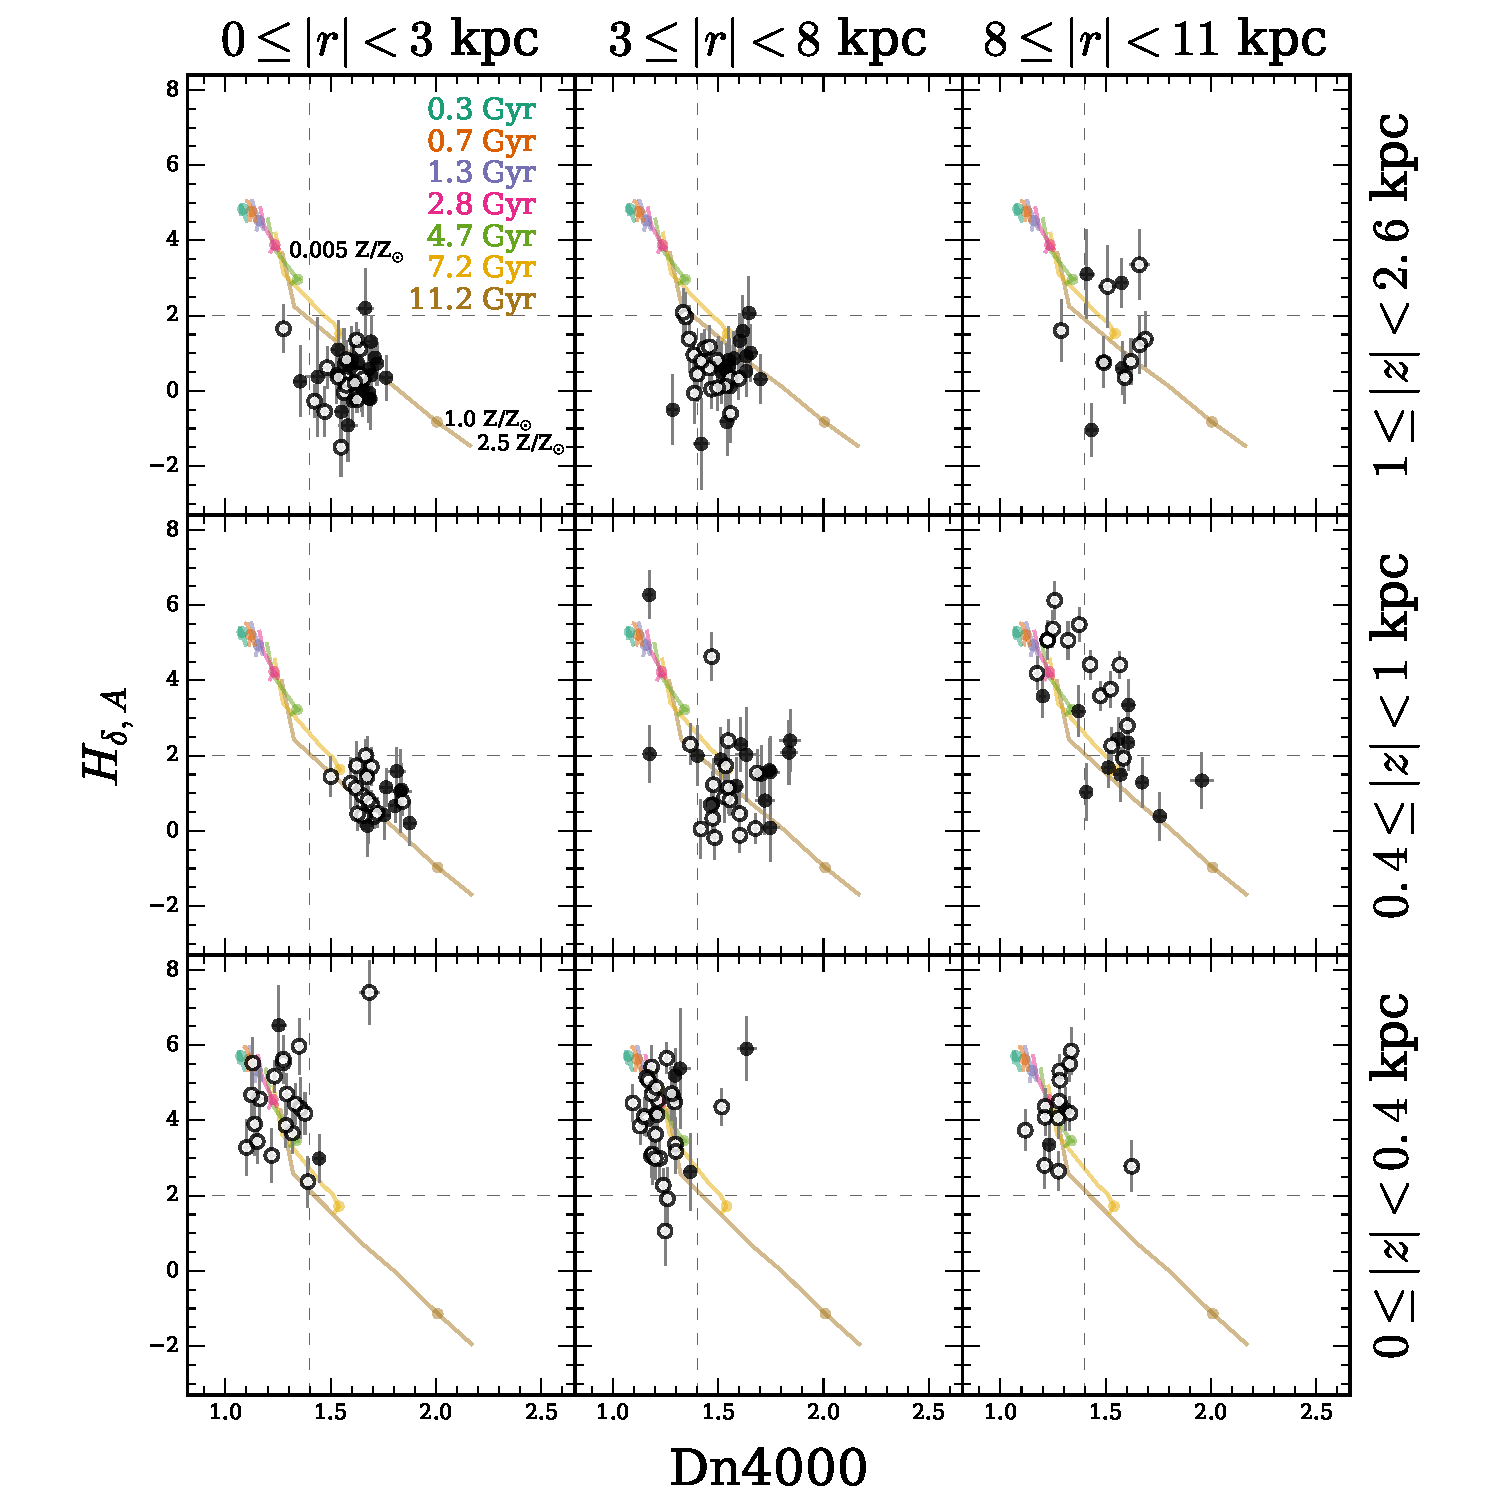
\includegraphics[width=0.8\textwidth]{891_1/figs/Dn4000_multires.pdf}
  \caption[$D_n(4000)$ vs \Hda in radius and height
  bins]{\label{891_1:fig:D4000_cuts}\fixspacing Spectral indices \Hda and
    $D_n(4000)$ for all good apertures in NGC 891 as a function of
    projected radius and height. Rationale for radial and vertical
    bins is provided in the text. Open symbols are for apertures on
    the approaching side, while filled circles are for apertures the
    receding side. Color-coded isochrones, labeled by their mean,
    light-weighted age at 5550 \AA\ are based on models with
    exponentially declining star-formation and a total age of 12 Gyr,
    as described in \S\ref{891_1:sec:fidgrid}; these are shown to
    highlight trends in age and the dependence of these indices on
    metallicity. The extreme values of metallicity are shown at the
    ends of the oldest isochrone in the top-left panel; solar
    metallicity for each isochrone is marked with a filled circle in
    all panels. The model values are adjusted for the mean
    instrumental resolution of each vertical bin as described in the
    text. Dashed lines are fiducial to highlight trends in age.}
\end{figure*}

We use \Hda and $D_n(4000)$ as our primary age indicators. As noted by
\citet{Hamilton85} these two indices are generally anti-correlated and
are useful, when combined, as an estimator of population age because
of their sensitivity to different star-formation time-scales.
Historically, \Hda has been used with $B-R$ color
\citep[e.g.,][]{Couch87} to discriminate between different
star-formation scenarios involving bursts, but \citet{Balogh99} has
shown that $D_n(4000)$ works as a suitable alternative to color, as
one might expect based on the correlations shown in
\citet{Hamilton85}. In essence, $D_n(4000)$ is a narrow-band color
intermediate in the wavelength range spanned by $U-B$. Because of its
relatively narrow band-pass it is more immune from extinction effects,
say, than broad-band colors.

Figure \ref{891_1:fig:D4000_cuts} shows these measurements grouped into
three radial and three vertical bins. The radial bins are chosen to
sample the region within the inner truncation of the super-thin disk
($|r| < \val{3}{kpc}$), the super-thin disk itself ($\val{3}{kpc}\leq
|r| < \val{8}{kpc}$), and beyond the outer super-thing disk truncation
($\val{8}{kpc} \leq |r|$) \citep{Schechtman-Rook13}. Vertical bins
were chosen to illustrate the stratification seen in stellar
populations: below \val{0.4}{kpc} stellar light is dominated by young
populations with strong Balmer absorption, but above this height we
see old populations with weak Balmer absorption and a correspondingly
strong $D_n(4000)$ break.

Again, as we saw in the comparison of Figures \ref{891_1:fig:MW_heating} and
\ref{891_1:fig:mab_data}, the results in Figure \ref{891_1:fig:D4000_cuts} for
the vertical age gradients are qualitatively consistent with the basic
heating model tuned to the MW solar cylinder presented in
\S\ref{891_1:sec:introduction}. Our MW heating model predicts this
transition to occur at roughly the scale-height of the old, thin
disk. The exact value depends on the assumed star-formation history
and how the scale-height is measured (e.g., band-pass and number of
components). We can begin by assuming the star-formation histories are
comparable for the two galaxies. In NGC 891 we find a sharp transition
from young to old stellar populations at \val{0.4}{kpc}. This is very
close to the vertical exponential scale-height for a single component
stellar disk fit to the broad-band light profile; \citet{Xilouris99}
find values of ranging from 0.34 to 0.43 kpc from the $K$ to $B$
bands, accounting for attenuation. For comparison, the super-thin and
thin disk components measured in the near-infrared $K$ band are 0.16
and 0.47 kpc, respectively. It is reasonable to presume that the
super-thin and thin components correspond to the young and old thin
disks in NGC 891.

Radial age gradients are minimal at low heights, but above the
midplane we see evidence for younger stars at larger radii,
particularly on the approaching side where there is an excess of
H$\alpha$, as discussed in Section \ref{891_1:sec:obs}. This gradient is
most pronounced for $\val{0.4}{kpc} \leq |z| < \val{1}{kpc}$ but is
visible even at the largest heights.

Discounting the azimuthal asymmetry for a moment (here projected onto
radius on either side of the center), this radial trend is indicative
of inside-out disk formation combined with disk flaring as seen in
simulations of MW-like disks \citep[e.g.,][]{Martig14a}. There is
ample evidence in today's massive disk galaxies that such a scenario
may indeed be viable. For example, in the MW and NGC 891 there is
evidence for gas flaring in atomic and molecular gas \citep[e.g.,][for
  NGC 891]{Scoville93, Yim11}. There also is recent evidence for
stellar flaring in the MW \citep{Ness16} as seen for age-dated giant
stars from APOGEE \citep{Majewski15}. In the $z\sim1$ galaxy
population there is also ample evidence of inside-out disk formation
based on Hubble Space Telescope studies \citep[e.g.,][]{Nelson15},
even for MW-like masses \citep[e.g.,][]{vanDokkum13}. This growth
pattern appears to be part of a broader trend (in time and galaxy
type) of size evolution \citep[e.g.,][]{Shibuya15}, although the
interpretation is challenging given the complexity of present day
mass-size relations seen, e.g., by \citet{Lange15} in the GAMA survey.
Nonetheless, spatially resolved spectroscopic maps of nearby galaxies
clearly show age gradients in disks, with the outer parts of disks
being younger in a light-weighted sense
\citep{Sanchez-Blazquez14,Gonzalez-Delgado15}. What we are able to
resolve here, for the first time in a massive spiral galaxy external
to the MW, is the {\it vertical} structure of these radial gradients.

Now considering the azimuthal asymmetry in star-formation and spiral
arm projection, it is clear that this asymmetry is reflected in the
vertical and radial gradients in the mean stellar age as reckoned in a
light-weighted sense with the indices in Figure \ref{891_1:fig:D4000_cuts}.
At the very least this should provide a cautionary reminder that
interpreting the radial and vertical gradients of spectral indices in
terms of specific scenarios (e.g., disk flaring and inside-out growth)
is necessary but perhaps not sufficient proof of the scenario's
plausibility. In particular, the role of projection, especially in the
context of the spiral arms and extinction, needs to be accounted for
as well \citep[cf the relative excess of H$\alpha$ vs 24$\mu$
  emission, as discussed in][]{Kamphuis07b}. We will show elsewhere
that differential SFH as a function of radius (where the outer
portions of disks are younger but not thicker) can also lead to {\it
  apparent} flaring in integrated star-light of a constant-thickness
disk. While star counts can certainly distinguish between flaring and
radially modulating SFH scenarios, for galaxies beyond the reach of
resolved stellar populations, stellar kinematics is likely the only
recourse to resolve different physical scenarios.

% see ALT TEXT above

% The radial gradients are consistent with an inside-out view of
% galaxy disk formation {\bf OG inside out ref}. Studies of high
% redshift galaxies \citep{Nelson12,Nelson13,Nelson15} {\bf we could
% go crazy with refs here} have shown that many disk galaxies exhibit
% a higher specific star formation rate and larger \Ha equivalent
% widths at large radii. This is often attributed to quenching in the
% inner regions caused by AGN and feedback after the initial burst of
% star formation, and there is evidence that is phenomenon is only
% observed in higher mass galaxies ($M_{\ast} > 10^{10.5}M_{\odot}$)
% \citep{Pan15,others?}. Regardless of whether these high-redshift
% disk are progenitors of disks at $z=0$ there is still evidence for
% similar trends in the local universe
% \citep{Sanchez-Blazquez07,Sanchez-Blazquez14} {\bf again, many more
% refs available}; disk galaxies show a larger proportion of young
% vs. old stars at larger radii, compared to the central regions.

The model grid in Figure \ref{891_1:fig:D4000_cuts} also highlights the
degeneracy between age and metallicity. Each colored line corresponds
to an isochrone of a given mean light-weighted age with varying values
of metallicity. As age increases the metallicity dependence in \Hda
and $D_n(4000)$ also increases. At an age of \val{\asim 11}{Gyr} these
indices can vary by almost the entire dynamic range of our data just
by assuming a different value for metallicity.  This age-metallicity
degeneracy is somewhat ameliorated by considering a reduced range of
metallicity (between 0.2 and 2.5 \Zsol), which we will show next is
plausible. Moreover, despite these degeneracies there is still a clear
distinction between ``young'' and ``old'' populations across the
vertical cut at \val{0.4}{kpc}; it is the actual age of this cutoff
that depends on metallicity.

\subsection{Metallicity and Abundance Gradients}
\begin{figure*}
  \centering
  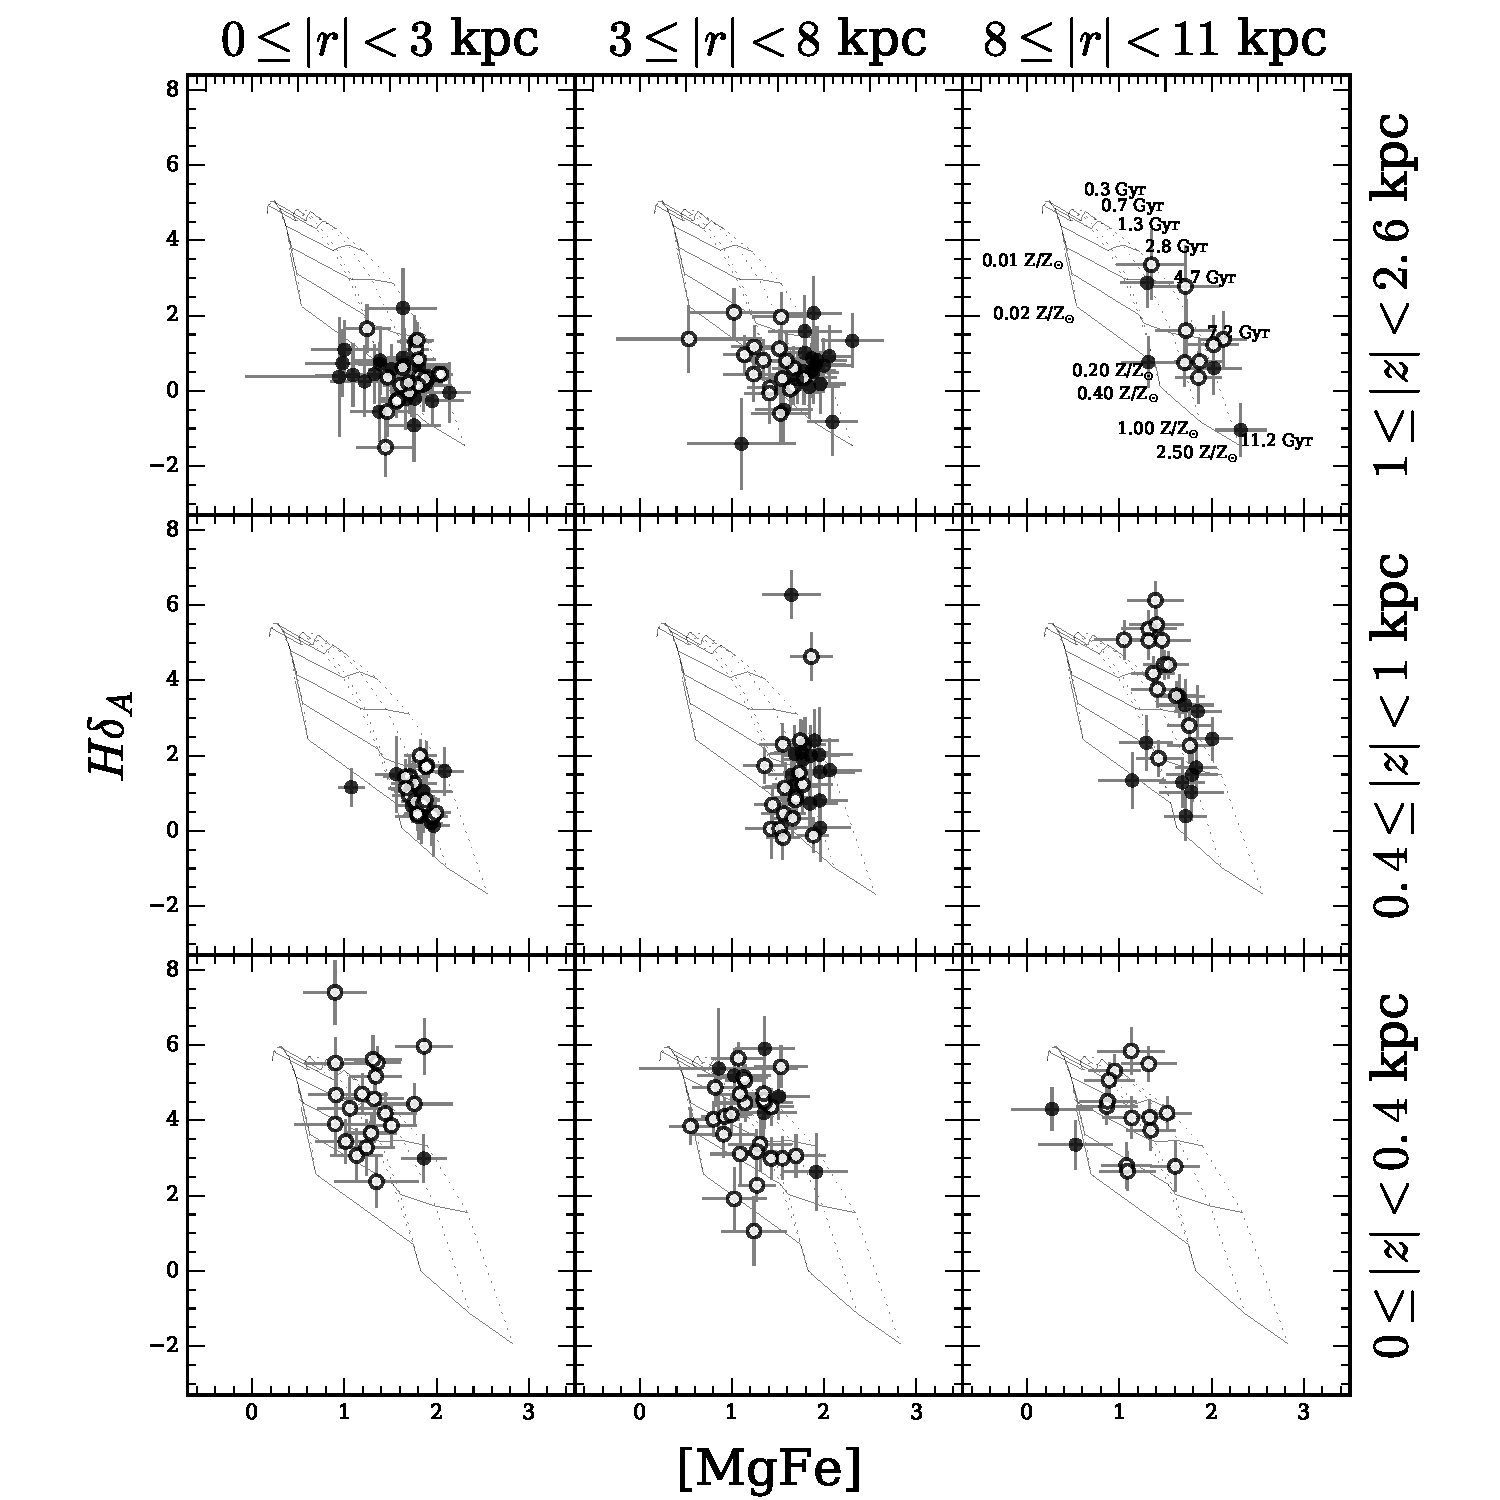
\includegraphics[width=0.8\textwidth]{891_1/figs/MgFe_multires.pdf}
  \caption[{[MgFe] vs \Hda in radius and height
    bins}]{\label{891_1:fig:MgFe_cuts}\fixspacing Spectral indices \Hda and
    [MgFe] for all apertures as a function of projected radius and
    height. Symbols, bins in radius and height, and models are the
    same as in Figure \ref{891_1:fig:D4000_cuts}. Lines of constant mean
    light-weighted age (isochrones, solid lines) and lines of constant
    metallicity (isofers, dotted lines) for the models are labeled in
    the top-right panel. The model values are adjusted for the mean
    instrumental resolution of each vertical bin as described in the
    text.}
\end{figure*}

Figure \ref{891_1:fig:MgFe_cuts} shows how metallicity (traced by [MgFe])
varies in the same bins defined in \S\ref{891_1:sec:age_grad} and Figure
\ref{891_1:fig:D4000_cuts}. Since [MgFe] is also age sensitive, we plot it
versus \Hda.  Guided by the fiducial grid described in
\S\ref{891_1:sec:fidgrid} we do not see significant trends in metallicity
with radius or height. The preponderance of apertures are well
described by metallicities in the range of $0.2 < Z/Z_\odot < 2.5$.

The lack of discernible gradients is perhaps unsurprising given the
precision of the measurements and the small dynamic range of the
indices, particularly for young ages. There are also line-of-sight
effects to consider as well. For example, there is a weak trend toward
slightly higher metallicities at intermediate heights. This may
appear counter-intuitive, but it may well reflect the confluence of
negative vertical and radial metallicity gradients and the fact that
as we move above the mid-plane the deprojected radii become smaller as
extinction diminishes.  In other words, all else being equal, young
formed near the center of a galaxy have higher metallicity than
young stars forming at large radii. Thus, at low heights where we
cannot see far into the disk we expect to find young populations with
low metallicity, but as height increases we can detect light from
smaller radii where the metallicity is on average higher.

While age gradients are again apparent in height Figure
\ref{891_1:fig:MgFe_cuts}, as too is the possible flaring of young stars
in the outer disk particularly on the approaching side, what is
also readily apparent is an asymmetry in the metallicity on the two
sides of the galaxy at intermediate radii. The receding side of the
galaxy, where there is less evidence for flaring, appears to be more
metal rich. This enhancement is most evident at intermediate and large
heights, i.e., for the older stars. This may also be a line-of-sight
depth effect in the sense that we are seeing farther in to the disk on
the receding side where, for a given height, metallicity is higher.

% We suspect our results stem from a combination of high optical depth
% at radial metallicity gradients. NGC 891 is known to be optically
% thick at optical wavelengths to heights of XXXX
% \citep{Xilouris99,Shcechtman-Rook12,?} so at low heights we can only
% observe populations at large radii. Furthermore, numerous studies of
% the Milky Way \citep{Hayden15,?,?} and external galaxies
% \citep{Ferguson98, vanZee98, ?} have shown that the metallicity of
% the ISM is anticorrelated with radius.
\begin{figure*}
  \centering
  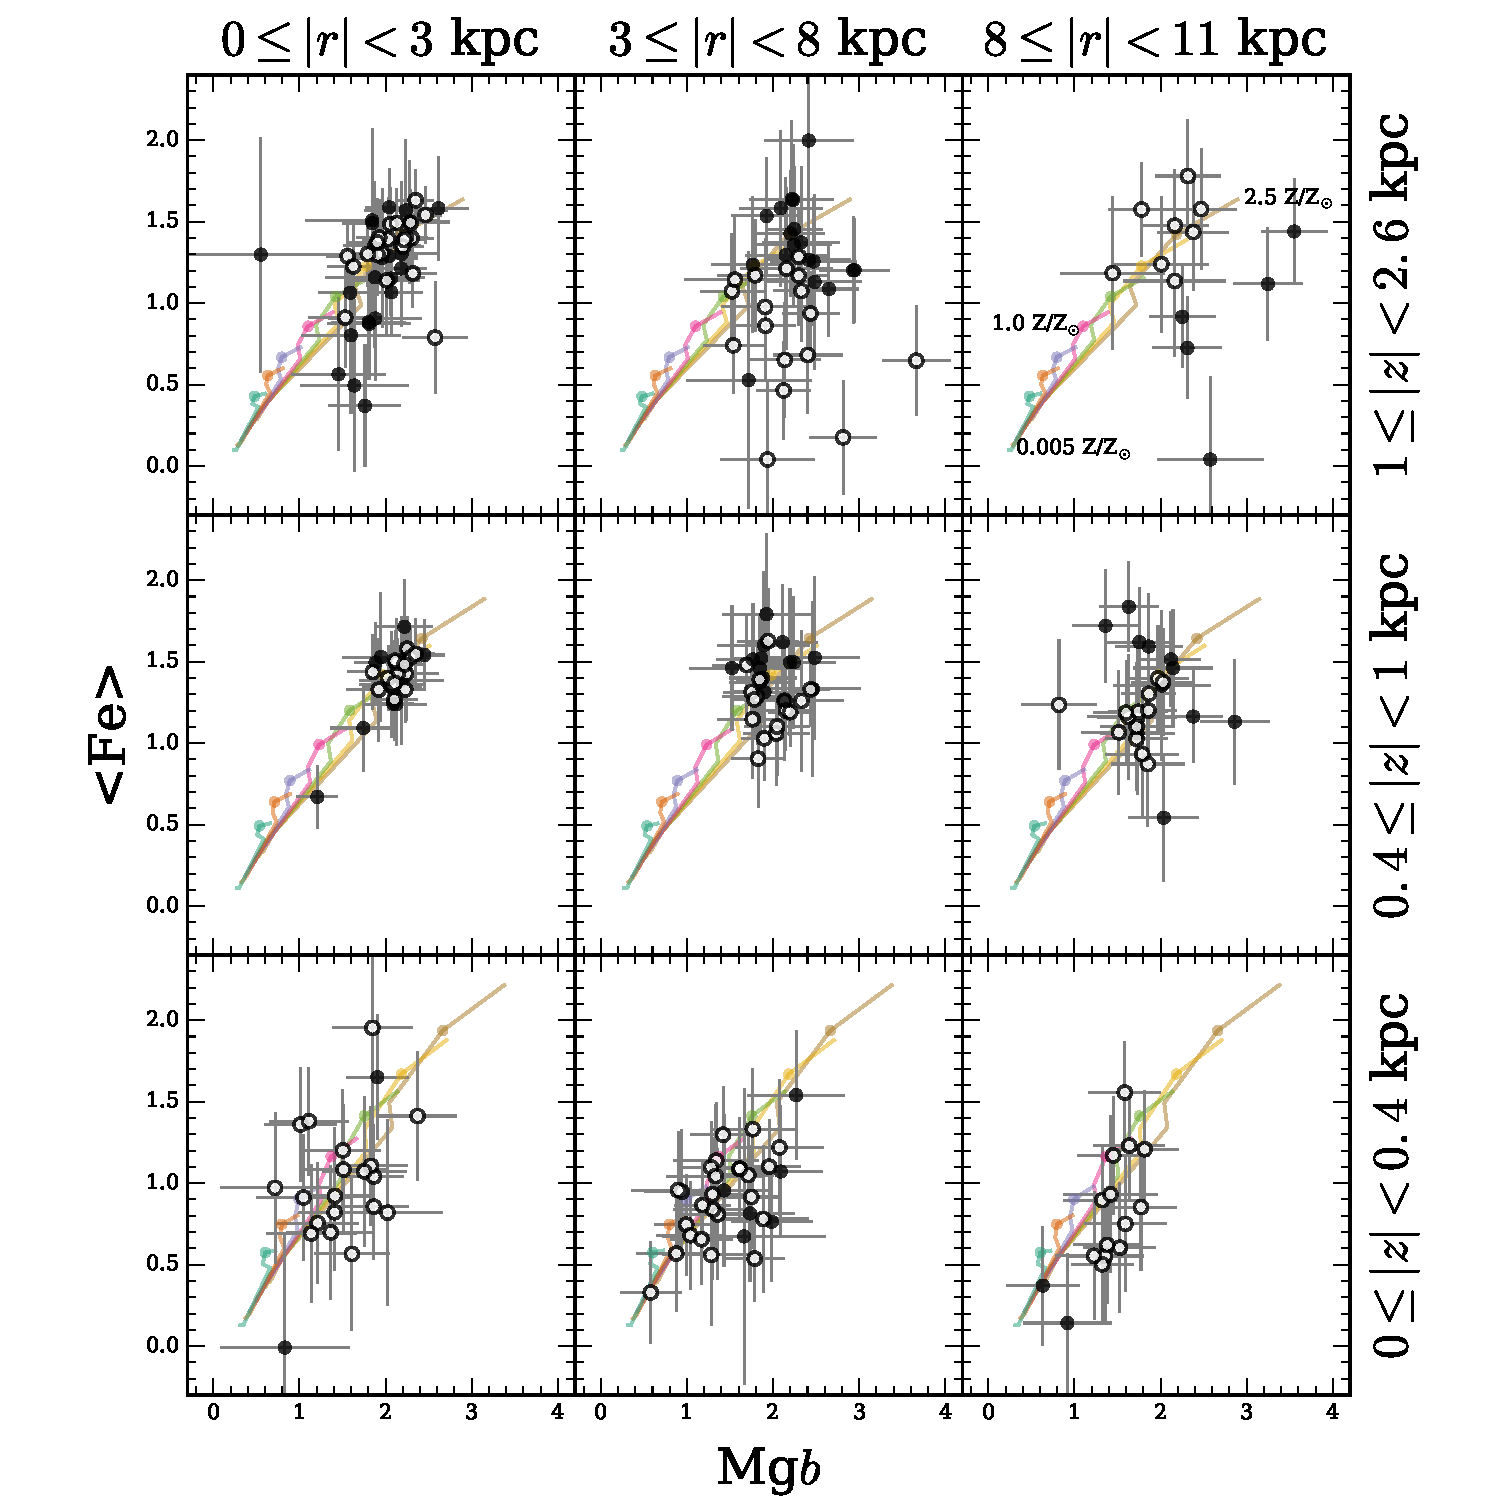
\includegraphics[width=0.8\textwidth]{891_1/figs/Mgb_multires.pdf}
  \caption[Mg$b$ vs $\left<\mathrm{Fe}\right>$ in radius and height
  bins]{\label{891_1:fig:Mgb_cuts}\fixspacing Spectral indices
    $\left<\mathrm{Fe}\right>$ and Mg$b$ for all apertures as a
    function of projected radius and height. Symbols, bins in radius
    and height, and model grid (including color-coding for age) are
    the same as in Figure \ref{891_1:fig:D4000_cuts}. The model values are
    adjusted for the mean instrumental resolution of each vertical bin
    as described in the text.}
\end{figure*}

In Figure \ref{891_1:fig:Mgb_cuts} we examine how abundance changes in our
data with radius and height. Based on the results of \citet{Thomas03}
(specifically their Figure 4) we note that populations with different
abundance will occupy different loci in the Mg$b$ vs
$\left<\mathrm{Fe}\right>$ plane, with higher abundance populations at
smaller values of $\left<\mathrm{Fe}\right>$ and slightly larger
values of Mg$b$. In general, increasing overall metallicity moves
points diagonally upward in this plot.

The differences in metallicity seen at intermediate radii and larger
heights in Figure \ref{891_1:fig:MgFe_cuts} appear to not have associated
abundance gradients.  There is some evidence for enhanced abundances
at low heights, and again at the largest heights. At intermediate
heights, where the errors are also the smallest, the abundances appear
to be very close to solar.

% The slope of the dashed lines in Figure \ref{fig:Mgb_cuts} is based on
% the distinction between high and low abundance models shown in
% \citet{Thomas03}.

%% The fiducial grid in this figure shows the Mg$b$ vs. <Fe>
%% plane is weakly sensitive to metallicity, but we caution that this
%% might be a result of a constant abundance {\bf WHAT IS IT?} across the
%% model galaxies used to construct it.
%% At low and intermediate heights
%% the abundance is remains constant while the age increases. Above
%% \val{1}{kpc}, however the age is relatively constant while the
%% abundance increases. This trend is especially prevelant at radii
%% beyond the inner portion of the galaxy.

% Below \val{1}{kpc} there is very little change in abundance with
% either radius or height, but above \val{1}{kpc} there is a clear
% transition to populations with a higher level of
% $\alpha$-enhancement. This is consistent with our claim of older
% populations at larger heights, but the fact that the transition in
% abundance occurs above the transition detected in Dn400 and \Hda
% indicates some mixing of populations between 0.4 and \val{1}{kpc}.

% Our conclusions that total metallicity and abundance respectively
% decrease and increase with height are generally consistent with
% detailed observations of the solar neighborhood
% \citep{Bovy12,Hayden15} and nearby galaxy disks
% \citep{Sanchez-Blazquez07}.

% \begin{figure*}
%   \centering
%   \includegraphics[width=\textwidth]{figs/index_height.pdf}
%   \caption{\label{fig:index_height}Each of the indices described in
%     \S\ref{891_1:sec:index_defn} plotted as a function of height above the
%     midplane. Vertical lines mark the borders of the vertical bins
%     shown in Figures \ref{fig:D4000_cuts} - \ref{fig:Mgb_cuts} and the
%     three radial bins used in the same figures are shown in different
%     colors. The transition from young to old populations at
%     \val{0.4}{kpc} is clear in the \Hda and $D_n4000$ panels. The three
%     lower panels show that abundance increases with height.}
% \end{figure*}
%
% [THIS IS THE TEXT THAT WENT WITH THE ABOVE FIGURE]
% Figure \ref{fig:index_height} shows the five indices measured above as
% a function of height above the midplane, where the transition from
% young to old populations is clearly visible at \val{0.4}{kpc} as
% measured in \Hda and $D_n4000$. Our primary abundance indicator,
% Mg$b$, also increases with height, but, interestingly, there is not as
% clear a break between high and low Mg$b$ values as there is with
% either $D_n4000$ or \Hda. However, coupled with a break to lower
% values of $\left<\mathrm{Fe}\right>$ above \val{1}{kpc} there is
% evidence of a high abundance population at these large heights,
% consistent with the results shown in Figure
% \ref{fig:Mgb_cuts}. Finally, we caution that, while it may appear the
% total metallicity increases with height, the [MgFe] index is highly
% dependent on age, as seen in Figure \ref{fig:MgFe_cuts}.

% \begin{figure*}
%   \centering
%   \includegraphics[width=\textwidth]{figs/repspec.pdf}
%   \caption{\label{fig:repspec}Binned spectra as a function of
%     projected radius and height. For each bin the spectrum is an
%     average of all apertures within the ($r,z$) limits shown, weighted
%     by the S/N of each aperture (see Table \ref{tab:data_ap}). At low
%     heights the spectra have strong \Hd absorption indicative of young
%     stellar populations, while larger heights show almost no \Hd
%     absorption but have a large break across \val{4000}{\AA}. The
%     results are qualitatively consistent with the heating referenced
%     in Figure \ref{fig:MW_heating}. Furthermore, at low heights there
%     is variation with radius, while at large heights the populations
%     seem to get slightly younger with increasing radius, perhaps
%     indicative of a flared disk.}
% \end{figure*}




\section{Summary}
\label{sec:summary}

We set out to measure vertical population gradients in NGC 891,
motivated to determine if the long-known vertical age gradients in our
solar neighborhood are seen in another spiral galaxy with comparable
rotation speed and morphology as the Milky Way.  The advent of large
spectroscopic surveys of Milky Way stars (see the Introduction) has
renewed interest in the age and metallicity gradients seen in the
Milky Way. Studies using these surveys
\citep[e.g.,][]{Bovy12c,Hayden14,Hayden15} are establishing the
relationships between age, velocity (height), metallicity and
compositional abundance of stars in unprecendent detail and accuracy,
but only for one galaxy.  Recent measurements have established the
age-velocity-metallicity relationshipn in M31's disk
\citep{Dorman15}. In this context we have undertaken to make the first
comrephensive deterimination of both vertical and radial population
gradients in integrated light for a massive spiral galaxy outside of
the Local Group.

To aid detailed studies of nearby galaxies like NGC 891 we constructed
a unique fiber integral field unit for the WIYN telescope's Bench
Spectrograph called \GP. \GP is part of a pair of variable-pitch IFUs
that share a common cable and spectrograph mount; the other IFU is
called HexPak, described elsewhere.  The \GP instrument is optimized
to measure vertical gradients in edge-on galaxies like NGC 891. In
this paper we have detailed the primary attributes of this instrument
relevant for astronomical observations, and we have presented
laboratory and on-telescope calibration of its performance.  The
unique design of this instrument required novel construction methods
that had some impact on its performance. In particular, the choice of
an aluminum fixture for \GP resulted in a sub-optimal polish for some
fibers that induced throughput losses (Appendix \ref{sec:GPtesting}),
however, the over-all performance of the IFU is quite high with a mean
throughput of 80\%.

The multi-pitch nature of \GP also required modifications to the
standard IFU data reduction routines, specifically flat-field and
absolute flux calibrations. We have shown (\S\ref{sec:data_reduction})
that these modifications do not significantly affect the quality of
the final data product. In fact, in the absence of atmospheric
dispersion correction, the presence of very large (6'' diameter)
fibers makes it possible to flux-calibrate \GP data very accurately in
both a relative and absolute sense ($\sim$5\%), as we have
demonstrated.

% Despite the learning curve associated with using a new type of
% instrument (here a variable pitch IFU), and the limitations of an
% outdated spectrograph, 

We have obtained spectroscopic observations of NGC 891 covering the
wavelength range from 337 to 764 nm, with high-quality data in the
range from 380 to 670 nm. Spectral resolution varies with wavelength
and fiber size in the range from 100 to 500 km s$^{-1}$; at 520 nm the
range is 180 to 350 km s$^{-1}$. Our spectroscopic maps span continuously
from the galaxy mid-lane to heights of 2.6 kpc, and sample projected
radii from 0.25 to 11 kpc from the center on {\it both} sides of the
disk. With these data we see clear trends in age with both projected
radius and height.

As a preliminary step in quantifying these age trends, and possible
trends in metallicity and abundance, we undertook measurement of
well-known spectroscopic indices including D$_n$4000 and the Lick
indices associated with Mgb, $<$Fe$>$, and [MgFe]. We have compared
these to standard, solar-abundance SPS models brought forward to the
resolution of the data and constructed for a range of on-going
star-formation. [For the purpose of exploring possible abundance
  variations we have also used models from Worthey for both solar and
  +0.3 dex solar abundances]. Our primary findings are:

% in O, Mg, Si, S, and Ca.

\begin{enumerate}
  \item There is a clear transition with height above NGC 891's disk
    midplane between young and old populations at \val{0.4}{kpc}
    (roughly the broad-band exponential scale-height), consistent with
    models of heating of the stellar in the Milky Way's Solar
    cylinder.

  \item For $|z| > \val{0.4}{kpc}$ there is a trend towards younger
    populations at larger projected radii, consistent with an
    inside-out formation history in NGC 891. The trend also suggests a
    flaring of the young stellar disk at radii beyond 8 kpc, which
    happens to be where \citet{Schechtman-Rook13} found an outer break
    in the super-thin (presumably star-forming) disk.

  \item Beyond 8 kpc in radius and between 0.4 kpc $\leq |z| <$ 1 kpc
    there is a a clear asymmetry in age between the two sides of the
    galaxy. The approaching side, where there is more H$\alpha$
    emission, appears younger. The extent to which this is an m=1
    asymmetry rather than a differential line-of-sight depth effect
    due to the (m=2) geometric arrangement of dust trailing stars and
    gas in spirals arms (as argued by \citet{Kamphuis07b} on the basis
    of 24$\mu$m emission) is not yet clear.  The gist of the argument
    against lpsided variations would be that the young-disk flaring
    between heights of 0.4 to 1 kpc is not as clearly seen on the
    receding side because these young stars are in a spiral arm
    projected behind a relative thick dust layer.  This suggests that
    better quantification of line-of-sight depth is needed to
    accurately interpret this asymmetry in the variation in vertical
    structure {\it within} NGC 891's disk.

\end{enumerate}

Secondary findings include there is little evidence for mean
metallicities outside the range of 0.2-2.5 \Zsol or abundances
outside the range of 0 to +0.3 dex of solar values. Changes in
metallicity and abundance are more difficult to quantify with these
small sets of indices, particularly given the relatively young ages at
low heights. There is a hint that metallicity increases slightly at
intermediate height, but we caution this may be modulated by
projection effects due to a negative metallicity gradient with radius
and increasing line-of-sight depth with height. There is evidence for
metallicity differences at the {\it same} height (above 0.4 kpc) and
{\it projected} radius (between 3 and 8 kpc) on either half of the
galaxy. Again, this may be a projection effect due to different
line-of-sight depths along the two halves of the galaxy, and in that
sense it may be related to the asymmetry seen in age versus height
beyond 8 kpc. However, if there is indeed a negative radial
metallicity gradient this would require the line-of-sight depth for
older stars to be somewhat larger on the receding side, which is
plausible given they will not be preferentially in spirals arms.

%   \item An increase in abundance and decrease in total metallicity
%     with height, consistent with measurements of the Milky Way and
%     nearby galaxies.

We stress that all of these measurements are {\it light}-weighted by
the very virtue of their observational nature, and hence are sensitive
to star-formation history (as we would like), and line-of-sight
depth. The latter is a considerable complication for edge-on galaxies,
and must be overcome for a detailed picture of the location of
different stellar populations in NGC 891 to emerge. The index
measurements reported above provide powerful qualitative measurements
of the general trends in stellar populations in NGC 891, but a
detailed quantitative assessment is hampered by degeneracies in age
and metallicity (see, for example, Figure \ref{fig:D4000_cuts}).  In
Paper II we employ full spectra fitting, guided by the results from
these indices, to reduce this degeneracy and make better quantitative
measurements of the population age as a function of both radius and
height. These measurements include extinction estimates and,
critically, kinematic estimates line-of-sight depth to our data in an
effort to de-project our radial measurements. What is robust from
these preliminary measurements, however, is the presence of vertical
age gradients in NGC 891 that appear much like what we see in the
Milky Way's disk.




\acknowledgements{We thank Guy Worthey for contributing his models of
  simple stellar populations as a function of age, metallicity and
  abundance. We thank Eric Hooper, as Interim WIYN Director, and
  Charles Corson for helping make the \GP installation possible; gift
  funds from the Department of Astronomy made this shipping and travel
  possible. This research was directly supported by the U.S. National
  Science Foundation (NSF) ATI-0804576, AST-1009471 and
  AST-1517006.}

\bibliographystyle{thesis}
\bibliography{ms_n891_paper}

%\chapter[Stellar Populations in NGC 891]{The Location of Stellar Populations in NGC 891}
\label{chap:891_pop}

% Leave space between title and quote or publication note.  This has often been
% 10cm for a quote and 8 cm for a reference, but this is really up to you.
%\vspace{8cm}

%%%%%%%%%%%%%%%%%%%%%%%%%%%%%%%%%%%%%%%%%%%%%%%%%%%%%%%%%%%%% 
%% \begin{chabstract}
%%     Chapter abstract.
%% \end{chabstract}
%% \cleardoublepage

\section{Outline}
Kind of the ``meat'' of the thesis. Here we go in depth about the analysis
methods used on the data described in \ref{chap:gradpak_obs}. The punchline is
some statement about how age (and, to a lesser precision, metallicty) varies
with radius and height in NGC 891.

\section{Basic Analysis}
\begin{itemize}
  \item Velocities
  \item Emission Correction
  \item Extinction Model
\end{itemize}
\subsection{Schedule}
This is basically done. The two things that still need work are 1) deciding
where exactly the extinction model section goes, and 2) basic editing. This
could be completed in 2 days.

\section{LOS Depths}
\begin{itemize}
  \item Velocity-based measurement
  \item Optical depth based measurement
\end{itemize}
\subsection{Schedule}
Great progress has been made over the last few days on this front. I think the
velocity stuff is done and 80\% written up.

The optical-depth section of this has a completed framework, but the analysis
depends on a lot of assumptions about the dust distribution that we will take
from other sources. This requires more thought. Still, a week should be
sufficient to complete this section.

\section{SSP Fitting}
\begin{itemize}
  \item Basic model
  \item Chisq weights
  \item Model Libraries
  \item Determining Age/Metallicity
\end{itemize}
\subsection{Schedule}
The first three bullet points above are basically done and need only basic
copy editing. This could be done in a few days.

The last bullet point is where we have been spending most of our time recently
and I think we are extremely close to being ``done'' with the actual
analysis. I mean, shit, we could say ``we're going to use weights because they
exclude known bad metallicities, and we're going to use this power because
we've sampled a coarse grid of powers and it does the best in terms of
rejecting metallicities, but not too many metallicities'' tomorrow and be done
with this. The pipline to produce ages and metallicities already exists, we're
just iterating on the uncertainties.

Once the anlysis is done this will take a week to write up.

\section{Spectral Indices}
\begin{itemize}
  \item Measurement
  \item Use as independent check on metallicities used in SSP fitting
  \item Qualitative results of trends in age, metallicity with height
\end{itemize}
\subsection{Schedule}
Some of this is already done. The last bullet point needs the most work. In
particular I have not settled on exactly what plane of spectral indices are
the most informative. Trager and Co. like Balmer vs <MgFe> and Balmer vs <Fe>,
but the latter of those does not work well with our galaxy models (dynamic
range is very small). We currently use \Hd vs <MgFe> and \Hd vs Mgb, but the
justification is lacking.

I think if we stay relatively shallow on this topic we can get everything
figured out relatively quickly. Maybe 1-2 weeks.

\section{Heating Models}
\begin{itemize}
  \item Model recipe
  \item comparison to data
\end{itemize}
\subsection{Schedule}
The ball is mostly in your court on this one. We have ages as a function of r
and z, now we need models for comparison. In principle this could be a very
short, ``look, we're not crazy'' section with an eye towards future, in depth
work.

\bibliographystyle{thesis}
\bibliography{891_pop}

\chapter[Doppler Tomography]{Decoding 3D Disk Struction and Dynamics Using Doppler Tomography}
\label{chap:SALT}

% Leave space between title and quote or publication note.  This has often been
% 10cm for a quote and 8 cm for a reference, but this is really up to you.
%\vspace{8cm}

%%%%%%%%%%%%%%%%%%%%%%%%%%%%%%%%%%%%%%%%%%%%%%%%%%%%%%%%%%%%% 
%% \begin{chabstract}
%%     Chapter abstract.
%% \end{chabstract}
%% \cleardoublepage

\section{Outline}
Hey, remember all the fun with SALT data? I sure do. We got pretty damn close
to having something cool a few times. I think the most concise and impactful
realization of this analysis was the stuff I present at Galaxies in 3D across
the Universe in Vienna, 2014.

\section{Schedule}
This is pretty tricky. If we want to persue any new analysis the potential for
lots of work becomes very high. I estimate that even just pulling together all
the basic information from various posters/proceedings/paper drafts into a
coherent chapter will take a week.

\bibliographystyle{thesis}
\bibliography{SALT}

\chapter[Conclusion]{Conclusion}
\label{chap:conclusion}

% Leave space between title and quote or publication note.  This has often been
% 10cm for a quote and 8 cm for a reference, but this is really up to you.
%\vspace{8cm}

%\vfil\eject\clearpage
\clearpage
NGC 891 offers a unique opportunity to perform stellar poulation
analyis and compare the results to our detailed understanding of the
distribution of stars in the Milky Way. In this way it occupies an
important bridge between the Milky Way and surveys that offer a large
sample size, but a smaller spatial resolution. The closeness and
nearly totally edge-on nature of NGC 891 also allows for unambiguous
determination of finely sampled vertical gradients in stellar
population, which makes it a perfect test-case for theories concerning
the origin of disk stratification seen in the Milky Way.

To take advantage of the information available in NGC 891 I helped
design and construct HexPak/\GP, a pair of fiber IFUs for the WIYN
telescope. In Chapter \ref{chap:pak_build} I detail the design and
fabrication of these instruments. The important features of HexPak/\GP
are:
\begin{enumerate}
\item HexPak has a standard hexagon shape made mostly of fibers with
  an on-sky diameter of 2\farcs8. It also has a high resolution core
  of 18 0\farcs94 fibers that make it idealy suited for studies of
  face-on galaxies or any bright object where high spatial resolution
  is desired.

\item \GP is roughly rectangular in shape and has five different fiber
  sizes ranging from 1\farcs87 - 5\farcs62. The regions of different
  size are arranged in a gradient that is optimized for to measure
  roughly expoentially decreasing surface brightness at roughly
  \val{10}{Mpc}; a similar S/N per fiber can be achieved in a single
  exposure. \GP is ideally suited for observations of objects with a
  large dynamic range in brightness where spectral resolution can be
  sacrificed for observing efficiency.

\item At the spectrograph input the slits of HexPak and \GP share a
  foot and focal plane. This allows observers to swap between the two
  IFUs with zero modifications to the Bench Spectrograph.

\item The head fixtures of HexPak and \GP, while physically separate,
  share a common focal plane in the WIYN IAS. This further eases the
  transition between the two IFUs. In practice an observer can switch
  between HexPak and \GP during an observing run in roughly 10
  minutes.

\end{enumerate}

During the conception and construction of HexPak/\GP I researched ways
to improve the optical performance of fiber-based instruments, mainly
through the mitigation of FRD. In Chapter \ref{chap:FRD} I detail my
experiements, which are broadly applicable to all fiber optic systems,
and find:
\begin{enumerate}

\item FRD is dominated by light entering the fiber at smaller angles
  (i.e., closer to the axis of light propogation).

\item A secondary component of FRD is attributable to the end-polish
  of fiber surfaces. FRD decreases with polishing down to finer grit
  sizes, but not significantly below grit-sizes of 5\mum.

\item Total throughput also depends on end-polish, with a wavelength
  dependence that indicates the increase in throughput is simply a
  reduction in surface-scattering.  The most significant gains occur
  for polishing that proceeds down to 5 $\mu$m grit, although for most
  astronomical applications at low light-levels polishing finer than
  this level is measurably advantageous.

\item The amount of FRD does \textbf{not} depend on wavelength.

\end{enumerate}

Chapter \ref{chap:891_1} details the first set of results from a
program that measures stellar populations in NGC 891 with \GP. In this
chapter I detail challenges in data acquisition/reduction caused by
the unique nature of \GP, but also present methods that largely
eliminate any negative impact on the resulting data.

I also describe the observing program that is designed to cover NGC
891 out to large heights and radii. The design of \GP is ideally
suited to a program of this nature and allows for efficient collection
of high-quality data.

I then use the well known and characterized LICK spectral index system
to identify separate stellar populations in NGC 891 and find:
\begin{enumerate}

\item There is a clear transition with height above NGC 891's disk
  midplane between young and old populations at \val{0.4}{kpc}
  (roughly the broad-band exponential scale-height). This is
  consistent with models of heating of the stellar disk in the solar
  cylinder.

  \item For $|z| > \val{0.4}{kpc}$ there is a trend towards younger
    populations at larger projected radii, consistent with an
    inside-out formation history in NGC 891. The trend also suggests a
    flaring of the young stellar disk at radii beyond 8 kpc.

  \item Beyond 8 kpc in radius and between 0.4 kpc $\leq |z| <$ 1 kpc
    there is a a clear asymmetry in age between the two sides of the
    galaxy. The approaching side, where there is more H$\alpha$
    emission, appears younger. This can be explained by spiral
    structure in NGC 891; on the approaching side of the galaxy we see
    the leading edge of a spiral arm that has very recent/ongoing star
    formation. Our sight-lines to the receeding side of the galaxy,
    however, look onto the trailing edge of another arm that is
    obscured by high concentrations of dust.

\end{enumerate}

Finally, in Chapter \ref{chap:891_2} I employ the power of
full-spectrum fitting to get a detailed and quantitaive view of
stellar populations in NGC 891. To confidently interpret the results
of this method I need to understand the interplay between all of the
fit parameters, namely the well known degeneracies between age,
metallicity, and extinction. Furthermore, assumptions about the star
formation history in NGC 891 can introduce large systematics in our
results.

The degeneracies between age, metallicity, and extinction are
exacerbated by SSP template libraries that constitute a large set of
individual SSPs with little thought to the astrophysical similarities
that exist over a wide range of age and metallicity values. In other
words, most SSP template libraries have many SSPs that, while assigned
different age or metallicity values, have very similar spectra. To
mitigate these degeneracies I use diffusion k-means to create a new
SSP basis set that greatly reduces the number of SSP templates while
still preserving important astrophysical features. With this new SSP
basis set I estimate the uncertainty in fit parameters caused by
degeneracies between the model spectra to be roughly 10\% for age and
extinction and \asim 20\% for metallicity.

I also quantify the systematic age uncertainty that arises from
assuming a star formation history during the interpretation of the
fitting results. In the worst case these uncertainties are \asim 20\%,
but I argue that the worst case (totally random star formation on
small physical scales) is unrealistically pessimistic for our
data. NGC 891 is a coherent galaxy and over long timescales (\asim 1
Gyr) the star formation history should be relatively the same across
the entire galaxy. Thus the systematic uncertainties do not apply when
comparing detailed structure within NGC 891; they are only important
when comparing NGC 891 to other galaxies that may have different star
formation histories.

With an understanding of uncertainties in my results I identify three
features in NGC 891 that are distinct from one another in a position,
age, metallicity, extinction phase space. They are:
\begin{enumerate}

\item A ``primary'' disk that exists at all heights and radii less
  than \val{8}{kpc}. In this disk there is clear evidence for the
  presence of young stellar populations ($< \val{\asim 400}{Myr}$ ago)
  below \val{0.4}{kpc} and a lack of the same populations above
  \val{0.4}{kpc}, consistent with the results of Chapter
  \ref{chap:891_1}. Above this transition emission from the disk is
  dominated by intermediate and old stars and the average population
  age increases with height. This disk also exhibits negative
  metallicity gradients with both radius and height, which is
  consistent with observations of the Milky Way. It is also likely
  that the primary ``disk'' is actually a superposition of multiple
  disk components previously identified in NGC 891.

\item A flared extension of the the primary disk at radii beyond
  \val{8}{kpc}. This flare has the same age and metallicity properties
  as the main disk, but with a scale height roughly twice as
  large. This increase in scale height decreases the total surface
  density of dust at large radii and the extinction is correspondingly
  lower, especially near the midplane.
  
\item A sequence of intermediate-age, super-solar metallicity
  populations at large heights ($|z|> \val{\asim 0.9}{kpc}$) and radii
  ($r>\val{8}{kpc}$). Despite their old ages, the populations in this
  ``third sequence'' appear to come from a fundamentally different
  underlying distribution compared to stars at similar heights but
  smaller radii. Despite an overall higher metallicity this third
  sequence still shows internal metallicity gradients in $r$, and $z$
  consistent with the trends seen in the primary disk and flare. The
  origin of this population is not easily explained and any theories
  about it will need to contend with its curious combination of old
  ages and high metallicities that occur far from the center of the
  galaxy.

\end{enumerate}

This work constitutes one of the first detailed, resolved studies of
stellar populations in a nearby galaxy and as such lays the groundwork
for future studies. In particular, the methods outlined here could
easily be applied to other nearby, edge-on galaxies. This thesis
provides a robust set of tools, from instruments to data reduction and
analysis methods, that will allow future astronomers to rapidly expand
our view of stellar populations and disk formation.

\clearpage
\phantomsection % Fixes references link in hyperref/PDF index

% Requires thesis.bst to be present (or linked) in chapter subdirectory.
\bibliographystyle{thesis}
\bibliography{Introduction}


% See the thesis.cls file for the steps to convert AASTeX papers
% into thesis chapters

%%%%% ADD APPENDICES %%%%%%%%%%%%%%%%%%%%%%%%%%%%%%%%%%%%%%%%%%%%%%%%%%%%%%%%%%%

% The \GP, like it's namesake, is difficult to construct, causes pain
% and suffering, but ultimately leads to an understanding of the
% universe that was previously unobtainable
%
% Facts to motivate drink
% o Layers
% o bottom has lower throughput (darker??)
% o sky bundles = some sort of "calibration" shooter?
% o possible southwest connection
%
% Layered pseudo-Zombie??


%\addtocontents{toc}{\protect\vspace{0.5cm}}
                        % Add some vertical space to the table of contents
                        %   file before listing the appendices (the \protect
                        %   command is necessary because \vspace is fragile).

%\appendix		% Resets chapter numbering to A, B, C... for appendices

%\include{apA}		% *.tex file for Appendix A (just like a chapter)

%\include{vitae}         % *.tex file for the Vitae

%\include{colophon}      % *.tex file for the Colophon

% END THE DOCUMENT %%%%%%%%%%%%%%%%%%%%%%%%%%%%%%%%%%%%%%%%%%%%%%%%%%%%%%%%%%%%%

%\clearpage
%Need to uncomment all of the following to get an index
%\addcontentsline{toc}{section}{Index}
%{\fixspacing \small
%\printindex
%}

\end{document}
